\documentclass{mimosis}

%%%%%%%%%%%%%%%%%%%%%%%%%%%%%%%%%%%%%%%%%%%%%%%%%%%%%%%%%%%%%%%%%%%%%%%%%%%%%%%
% External import 
%%%%%%%%%%%%%%%%%%%%%%%%%%%%%%%%%%%%%%%%%%%%%%%%%%%%%%%%%%%%%%%%%%%%%%%%%%%%%%%


%%%%%%%%%%%%%%%%%%%%%%%%%%%%%%%%%%%%%%%%%%%%%%%%%%%%%%%%%%%%%%%%%%%%%%%%%%%%%%%
% Basic packages
%%%%%%%%%%%%%%%%%%%%%%%%%%%%%%%%%%%%%%%%%%%%%%%%%%%%%%%%%%%%%%%%%%%%%%%%%%%%%%%

\usepackage[utf8]{inputenc}                                 % allow utf-8 input
\usepackage[T1]{fontenc}                                    % use 8-bit T1 fonts
\usepackage{url}                                            % simple URL typesetting
\usepackage{microtype}                                      % microtypography
\usepackage{calc}                                           % perform arithmetic on the arguments
\usepackage{xspace}                                         % commands that appear not to eat spaces
\usepackage{enumitem}                                       % control layout of itemize, enumerate
\usepackage{numprint}                                       % prints numbers with a separator every three digits
\usepackage{epigraph}                                       % for citation
\usepackage[super]{nth}                                     % Generate English ordinal numbers
\usepackage{bbding}                                         % A symbol font
\usepackage[title, toc, titletoc, page, header]{appendix}   % extra control of appendices
\usepackage{lmodern}
\usepackage{psl-cover}                                      % package for PSL cover
\usepackage{etoc}                                           % Support for Mini Table of Contents
\usepackage{etoolbox}                                       % toolbox
\usepackage[binary-units=true]{siunitx}                     % A comprehensive (SI) units package

%%%%%%%%%%%%%%%%%%%%%%%%%%%%%%%%%%%%%%%%%%%%%%%%%%%%%%%%%%%%%%%%%%%%%%%%%%%%%%%
% Mathematical packages
%%%%%%%%%%%%%%%%%%%%%%%%%%%%%%%%%%%%%%%%%%%%%%%%%%%%%%%%%%%%%%%%%%%%%%%%%%%%%%%

\usepackage{mathtools}      % Mathematical tools to use with amsmath
\usepackage{amssymb}
\usepackage{amsthm}         % Basic mathematical environments for proofs etc.
\usepackage{mathdots}       % dots commands for matrices 
\usepackage{amsfonts}       % blackboard math symbols
\usepackage{nicefrac}       % compact symbols for 1/2, etc.
\usepackage{physics}        % typesetting equations for physics simpler
\usepackage{bm}             % Access bold symbols in maths mode
\usepackage{centernot}      % The package provides \centernot
\usepackage{thmtools}       % Extensions to theorem environments
\usepackage{afterpage}

%%%%%%%%%%%%%%%%%%%%%%%%%%%%%%%%%%%%%%%%%%%%%%%%%%%%%%%%%%%%%%%%%%%%%%%%%%%%%%%
% Graphics packages
%%%%%%%%%%%%%%%%%%%%%%%%%%%%%%%%%%%%%%%%%%%%%%%%%%%%%%%%%%%%%%%%%%%%%%%%%%%%%%%

\usepackage{pgfplots}
\usepackage{graphicx}       % enhanced support for graphics
\usepackage{tikz}           % create graphic elements in latex
\usepackage{tikz-cd}        % Create commutative diagrams with TikZ
\usetikzlibrary{positioning}
\usetikzlibrary{arrows.meta}
\usepgfplotslibrary{groupplots}

%%%%%%%%%%%%%%%%%%%%%%%%%%%%%%%%%%%%%%%%%%%%%%%%%%%%%%%%%%%%%%%%%%%%%%%%%%%%%%%
% Table packages
%%%%%%%%%%%%%%%%%%%%%%%%%%%%%%%%%%%%%%%%%%%%%%%%%%%%%%%%%%%%%%%%%%%%%%%%%%%%%%%

\usepackage{array}          % extending the array and tabular environments
\usepackage{multirow}       % create tabular cells spanning multiple rows
\usepackage{tabularx}       % tabulars with adjustable-width columns
\usepackage{booktabs}       % professional-quality tables
\usepackage{makecell}

% This ensures that I am able to typeset bold font in table while still aligning the numbers correctly.
\DeclareSIUnit\px{px}
\sisetup{%
  separate-uncertainty,
  detect-all           = true,
  detect-family        = true,
  detect-mode          = true,
  detect-shape         = true,
  detect-weight        = true,
  detect-inline-weight = math,
  multi-part-units     = single
}

\newcolumntype{L}[1]{>{\raggedright\arraybackslash}p{#1}}
\newcolumntype{C}[1]{>{\centering\arraybackslash}p{#1}}

% Switch Tableau for French chapter
\addto\captionsfrench{\def\tablename{Tableau}}
% \DefineBibliographyExtras{french}{\restorecommand\mkbibnamefamily}



%%%%%%%%%%%%%%%%%%%%%%%%%%%%%%%%%%%%%%%%%%%%%%%%%%%%%%%%%%%%%%%%%%%%%%%%%%%%%%%
% Hyperlinks
%%%%%%%%%%%%%%%%%%%%%%%%%%%%%%%%%%%%%%%%%%%%%%%%%%%%%%%%%%%%%%%%%%%%%%%%%%%%%%%

\definecolor{mydarkblue}{rgb}{0.02, 0.40, 0.62}
\usepackage[
  colorlinks=true,
  allcolors=mydarkblue,
  ]{hyperref}
\usepackage{cleveref}       % Intelligent cross-referencing
\usepackage{bookmark}       % Bookmarks in the resulting PDF


%%%%%%%%%%%%%%%%%%%%%%%%%%%%%%%%%%%%%%%%%%%%%%%%%%%%%%%%%%%%%%%%%%%%%%%%%%%%%%%
% Algoithms
%%%%%%%%%%%%%%%%%%%%%%%%%%%%%%%%%%%%%%%%%%%%%%%%%%%%%%%%%%%%%%%%%%%%%%%%%%%%%%%

% should be loaded after hyperref
\usepackage[chapter]{algorithm} % Support for typesetting algorithms
\usepackage{algpseudocode}      % Support for typesetting pseudocode

\makeatletter
\newcounter{algorithmicH}% New algorithmic-like hyperref counter
\let\oldalgorithmic\algorithmic
\renewcommand{\algorithmic}{%
  \stepcounter{algorithmicH}% Step counter
  \oldalgorithmic}% Do what was always done with algorithmic environment
\renewcommand{\theHALG@line}{ALG@line.\thealgorithmicH.\arabic{ALG@line}}
\makeatother


%%%%%%%%%%%%%%%%%%%%%%%%%%%%%%%%%%%%%%%%%%%%%%%%%%%%%%%%%%%%%%%%%%%%%%%%%%%%%%%
% Parameters
%%%%%%%%%%%%%%%%%%%%%%%%%%%%%%%%%%%%%%%%%%%%%%%%%%%%%%%%%%%%%%%%%%%%%%%%%%%%%%%

% Fonts
\DeclareFontFamily{T1}{calligra}{}
\DeclareFontShape{T1}{calligra}{m}{n}{<->s*[1.44]callig15}{}
\DeclareMathAlphabet\mathcalligra   {T1} {calligra} {m}  {n}
\DeclareMathAlphabet\mathzapf       {T1} {pzc}      {mb} {it}
\DeclareMathAlphabet\mathchorus     {T1} {qzc}      {m}  {n}
\DeclareMathAlphabet\mathrsfso      {U}  {rsfso}    {m}  {n}

\DeclareUnicodeCharacter{2212}{-}

% Minitoc
\newlength\tocrulewidth
\setlength{\tocrulewidth}{0.8pt}
\etocsettocstyle{
  \addsec*{Contents \\ \vspace{-0.5cm}
    \rule{\textwidth}{\tocrulewidth}
    \vspace{-1cm plus0mm minus0mm}
  }
}{
  \noindent\rule{\linewidth}{\tocrulewidth}
}

\newcommand{\localtoc}{
  \begingroup
    \localtableofcontents
    % \vspace{1cm}
  \endgroup
}


%%%%%%%%%%%%%%%%%%%%%%%%%%%%%%%%%%%%%%%%%%%%%%%%%%%%%%%%%%%%%%%%%%%%%%%%%%%%%%%
% Bibliography
%%%%%%%%%%%%%%%%%%%%%%%%%%%%%%%%%%%%%%%%%%%%%%%%%%%%%%%%%%%%%%%%%%%%%%%%%%%%%%%

\usepackage[%
  style        = authoryear-comp, % autocite=inline, sortcites=true, labeldateparts=true, uniquename=full, uniquelist=true.
  backend      = biber,
  autocite     = plain,
  uniquename   = false,
  uniquelist   = false,
  sorting      = ynt,
  sortcites    = true,
  doi          = false,
  url          = false,
  giveninits   = true,
  hyperref     = true,
  maxbibnames  = 99,
  maxcitenames = 2,
  natbib       = true,
  backref      = true,
  abbreviate   = true,
  dashed       = false,
  ]{biblatex}

\makeatletter
\let\abx@macro@citeOrig\abx@macro@cite
\renewbibmacro{cite}{%
  \bibhyperref{%
  \let\bibhyperref\relax\relax%
  \abx@macro@citeOrig%
    }%
}

% code that fix the color of the last bracket
% https://tex.stackexchange.com/a/25972
\DeclareCiteCommand{\textcite}
 {\boolfalse{cbx:parens}}
  {\usebibmacro{citeindex}%
    \printtext[bibhyperref]{\printnames{labelname}%
      \printtext{ (\printfield{year}\printtext{)}}}}
 {\ifbool{cbx:parens}
  {\bibcloseparen\global\boolfalse{cbx:parens}}
  {}%
 \textcitedelim}
{\usebibmacro{textcite:postnote}}
\makeatother

\DefineBibliographyStrings{english}{and={and}}
\DefineBibliographyStrings{english}{in={in}}
\DefineBibliographyStrings{english}{page={page}}
\DefineBibliographyStrings{english}{pages={pages}}
\DefineBibliographyStrings{english}{andothers={et al.}}
\DefineBibliographyStrings{english}{byeditor={editor}}
\DefineBibliographyStrings{english}{volume={volume}}
\DefineBibliographyStrings{english}{backrefpage={see page}}
\DefineBibliographyStrings{english}{backrefpages={see pages}}
\DefineBibliographyStrings{english}{phdthesis={PhD Thesis}}
\renewcommand{\cite}[1]{\citep{#1}}
\renewcommand{\finalnamedelim}{ \& }
\renewcommand{\textcitedelim}{
  \iflastcitekey{
    \unspace\textcolor{black}{\text{\ and}}\unspace
  }{
  \addcomma}\space}

%%%%%%%%%%%%%%%%%%%%%%%%%%%%%%%%%%%%%%%%%%%%%%%%%%%%%%%%%%%%%%%%%%%%%%%%
% Some adjustments to make the bibliography more clean
%%%%%%%%%%%%%%%%%%%%%%%%%%%%%%%%%%%%%%%%%%%%%%%%%%%%%%%%%%%%%%%%%%%%%%%%
%
% The subsequent commands do the following:
%  - Removing the month field from the bibliography
%  - Fixing the Oxford commma
%  - Suppress the "in" for journal articles
%  - Remove the parentheses of the year in an article
%  - Delimit volume and issue of an article by a colon ":" instead of
%    a dot ""
%  - Use commas to separate the location of publishers from their name
%  - Remove the abbreviation for technical reports
%  - Display the label of bibliographic entries without brackets in the
%    bibliography
%  - Ensure that DOIs are followed by a non-breakable space
%  - Use hair spaces between initials of authors
%  - Make the font size of citations smaller
%  - Fixing ordinal numbers (1st, 2nd, 3rd, and so) on by using
%    superscripts

% Remove the month field from the bibliography. It does not serve a good
% purpose, I guess. And often, it cannot be used because the journals
% have some crazy issue policies.
\AtEveryBibitem{\clearfield{month}}
\AtEveryCitekey{\clearfield{month}}

% Fixing the Oxford comma. Not sure whether this is the proper solution.
% More information is available under [1] and [2].
%
% [1] http://tex.stackexchange.com/questions/97712/biblatex-apa-style-is-missing-a-comma-in-the-references-why
% [2] http://tex.stackexchange.com/questions/44048/use-et-al-in-biblatex-custom-style
%
\AtBeginBibliography{%
  \renewcommand*{\finalnamedelim}{%
    \ifthenelse{\value{listcount} > 2}{%
      \addcomma
      \addspace
      \bibstring{and}%
    }{%
      \addspace
      \bibstring{and}%
    }
  }
}

% Suppress "in" for journal articles. This is unnecessary in my opinion
% because the journal title is typeset in italics anyway.
\renewbibmacro{in:}{%
  \ifentrytype{article}
  {%
  }%
  % else
  {%
    \printtext{\bibstring{in}\intitlepunct}%
  }%
}

% Remove the parentheses for the year in an article. This removes a lot
% of undesired parentheses in the bibliography, thereby improving the
% readability. Moreover, it makes the look of the bibliography more
% consistent.
\renewbibmacro*{issue+date}{%
  \setunit{\addcomma\space}
    \iffieldundef{issue}
      {\usebibmacro{date}}
      {\printfield{issue}%
       \setunit*{\addspace}%
       \usebibmacro{date}}%
  \newunit}

% Delimit the volume and the number of an article by a colon instead of
% by a dot, which I consider to be more readable.
\renewbibmacro*{volume+number+eid}{%
  \printfield{volume}%
  \setunit*{\addcolon}%
  \printfield{number}%
  \setunit{\addcomma\space}%
  \printfield{eid}%
}

% Do not use a colon for the publisher location. Instead, connect
% publisher, location, and date via commas.
\renewbibmacro*{publisher+location+date}{%
  \printlist{publisher}%
  \setunit*{\addcomma\space}%
  \printlist{location}%
  \setunit*{\addcomma\space}%
  \usebibmacro{date}%
  \newunit%
}

% Ditto for other entry types.
\renewbibmacro*{organization+location+date}{%
  \printlist{location}%
  \setunit*{\addcomma\space}%
  \printlist{organization}%
  \setunit*{\addcomma\space}%
  \usebibmacro{date}%
  \newunit%
}

% Do not abbreviate "technical report".
\DefineBibliographyStrings{english}{%
  techreport = {technical report},
}

% Display the label of a bibliographic entry in bare style, without any
% brackets. I like this more than the default.
%
% Note that this is *really* the proper and official way of doing this.
\DeclareFieldFormat{labelnumberwidth}{#1\adddot}

% Ensure that DOIs are followed by a non-breakable space.
\DeclareFieldFormat{doi}{%
  \mkbibacro{DOI}\addcolon\addnbspace
    \ifhyperref
      {\href{http://dx.doi.org/#1}{\nolinkurl{#1}}}
      %
      {\nolinkurl{#1}}
}

% Use proper hair spaces between initials as suggested by Bringhurst and
% others.
\renewcommand*\bibinitdelim {\addnbthinspace}
\renewcommand*\bibnamedelima{\addnbthinspace}
\renewcommand*\bibnamedelimb{\addnbthinspace}
\renewcommand*\bibnamedelimi{\addnbthinspace}

% Make the font size of citations smaller. Depending on your selected
% font, you might not need this.
\renewcommand*{\citesetup}{%
  \biburlsetup
  \small
}

\DeclareLanguageMapping{british}{bibliography-correct-ordinals}
\DeclareLanguageMapping{english}{bibliography-correct-ordinals}

\addbibresource{bibliography/springer.bib}
\addbibresource{bibliography/neurips.bib}
\addbibresource{bibliography/linear_algebra.bib}
\addbibresource{bibliography/aaai.bib}
\addbibresource{bibliography/icml.bib}
\addbibresource{bibliography/iclr.bib}
\addbibresource{bibliography/iccv.bib}
\addbibresource{bibliography/eccv.bib}
\addbibresource{bibliography/cvpr.bib}
\addbibresource{bibliography/arxiv.bib}
\addbibresource{bibliography/other.bib}

\setlength\bibitemsep{5pt}

% Fix citation when using French language
% https://tex.stackexchange.com/questions/53309/changing-default-citet-font-in-biblatex
\DefineBibliographyExtras{french}{\restorecommand\mkbibnamefamily}

%%%%%%%%%%%%%%%%%%%%%%%%%%%%%%%%%%%%%%%%%%%%%%%%%%%%%%%%%%%%%%%%%%%%%%%%%%%%%%%
% Theorems
%%%%%%%%%%%%%%%%%%%%%%%%%%%%%%%%%%%%%%%%%%%%%%%%%%%%%%%%%%%%%%%%%%%%%%%%%%%%%%%

\declaretheoremstyle[
  spaceabove=6pt, spacebelow=6pt,
  bodyfont=\itshape,
  postheadspace=1em,
  qed=,
]{style}

\declaretheoremstyle[
  spaceabove=6pt, spacebelow=6pt,
  bodyfont=\itshape,
  postheadspace=1em,
  qed=,
  shaded={
    rulecolor=mydarkblue,
    rulewidth=2pt,
    bgcolor=white,
    padding=0.02\textwidth,
    textwidth=0.96\textwidth},
]{maintheoremstyle}


\declaretheorem[
  numberwithin=chapter,
  name=Theorem,
  style=style,
  refname={theorem,theorems},
  Refname={Theorem,Theorems}]{theorem}
\declaretheorem[
  numberwithin=chapter,
  name=Corollary,
  style=style,
  refname={corollary,corollaries},
  Refname={Corollary,Corollaries}]{corollary}

\declaretheorem[
  numberwithin=chapter,
  name=Definition,
  style=style,
  refname={definition,definitions},
  Refname={Definition,Definitions}]{definition}
\declaretheorem[
  numberwithin=chapter,
  name=Lemma,
  style=style,
  refname={lemma,lemmas},
  Refname={Lemma,Lemmas}]{lemma}
\declaretheorem[
  numberwithin=chapter,
  name=Proposition,
  style=style,
  refname={proposition,propositions},
  Refname={Proposition,Propositions}]{proposition}
\declaretheorem[
  numberwithin=chapter,
  name=Problem,
  style=style,
  refname={problem,problems},
  Refname={Problem,Problems}]{problem}
\declaretheorem[
  numberwithin=chapter,
  numbered=no,
  name=Remark,
  style=style,
  refname={remark,remarks},
  Refname={Remark,Remarks}]{remark}

\declaretheorem[
  numberwithin=chapter,
  name=Theorem,
  style=maintheoremstyle,
  sibling=theorem,
  refname={theorem,theorems},
  Refname={Theorem,Theorems}]{maintheorem}
\declaretheorem[
  numberwithin=chapter,
  name=Corollary,
  style=maintheoremstyle,
  sibling=corollary,
  refname={corollary,corollaries},
  Refname={Corollary,Corollaries}]{maincorollary}

\declaretheorem[
  numberwithin=chapter,
  numbered=no,
  name=Property,
  style=style,
  refname={property,properties},
  Refname={Property,Properties}]{property}
\declaretheorem[
  numberwithin=chapter,
  numbered=no,
  name=Properties,
  style=style,
  refname={property,properties},
  Refname={Property,Properties}]{properties}


\let\proof\relax
\let\endproof\relax

\declaretheoremstyle[
  notebraces={}{},
  headfont=\bfseries\itshape,
  notefont=\bfseries\itshape,
  postheadspace=1em,
  postfoothook=\vspace{2em},
  qed=$\blacksquare$,
  mdframed={
    topline=false,
    bottomline=false,
    rightline=false,
    linecolor=lightgray,
    linewidth=3pt,
    backgroundcolor=white,
    innerleftmargin=0.02\textwidth,
    innerrightmargin=0pt,
  }
]{proofstyle}

\declaretheorem[
  numbered=no,
  name=Proof of,
  style=proofstyle,
  refname={proof,proofs},
  Refname={Proof,Proofs}
]{proof}



%%%%%%%%%%%%%%%%%%%%%%%%%%%%%%%%%%%%%%%%%%%%%%%%%%%%%%%%%%%%%%%%%%%%%%%%%%%%%%%
% Text commands
%%%%%%%%%%%%%%%%%%%%%%%%%%%%%%%%%%%%%%%%%%%%%%%%%%%%%%%%%%%%%%%%%%%%%%%%%%%%%%%

\newcommand{\yt}    {\textit{\mbox{YouTube-8M}}\xspace}
\newcommand{\eg}    {\textit{e.g.}\xspace}
\newcommand{\ie}    {\textit{i.e.}\xspace}
\newcommand{\cf}    {\textit{cf.}\xspace}
\newcommand{\aka}   {\textit{a.k.a.}\xspace}
\newcommand{\pdf}   {p.d.f.\xspace}
\newcommand{\st}    { s.t.\xspace}
\newcommand{\vs}    {\textit{vs.}\xspace}
\newcommand{\wrt}   {w.r.t.\xspace}


%%%%%%%%%%%%%%%%%%%%%%%%%%%%%%%%%%%%%%%%%%%%%%%%%%%%%%%%%%%%%%%%%%%%%%%%%%%%%%%
% Specific Operators
%%%%%%%%%%%%%%%%%%%%%%%%%%%%%%%%%%%%%%%%%%%%%%%%%%%%%%%%%%%%%%%%%%%%%%%%%%%%%%%

\DeclareMathOperator*{\argmax}       {arg\,max}
\DeclareMathOperator*{\argmin}       {arg\,min}
\DeclareMathOperator*{\Ebb}          {\mathbb{E}}
\DeclareMathOperator*{\Pbb}          {\mathbb{P}}
\DeclareMathOperator*{\Risk}         {Risk}
\DeclareMathOperator*{\advRisk}      {Risk_{\alpha}}
\DeclareMathOperator*{\PCadvRisk}    {PC-Risk_{\alpha}}
\DeclareMathOperator*{\randRisk}     {Rand-Risk}
\DeclareMathOperator*{\randadvRisk}  {Rand-Risk_{\alpha}}
\DeclareMathOperator*{\ranfPCadvRisk}{Rand-PC-Risk_{\alpha}}
\DeclareMathOperator*{\B}            {B(\alpha)}
\DeclareMathOperator*{\probmap}      {M}
\DeclareMathOperator*{\EoT}          {EoT}
\DeclareMathOperator*{\Vol}          {Vol}

% \relax\vec
% \renewcommand{\vec}    {\ensuremath{\mathrm{vec}}\xspace}
\newcommand{\relu}     {\ensuremath{\mathrm{ReLU}}\xspace}
\newcommand{\pad}      {\ensuremath{\mathrm{pad}}\xspace}
\newcommand{\lipp}[2]  {\ensuremath{\mathrm{Lip}_{#1} \left(#2\right)}}
\newcommand{\lip}[1]   {\ensuremath{\mathrm{Lip}\left(#1\right)}}
\newcommand{\lipbound} {\ensuremath{\mathrm{LipBound}}}
\newcommand{\diag}     {\ensuremath{\mathrm{diag}}}
\newcommand{\bdiag}    {\ensuremath{\mathrm{bdiag}}}
\newcommand{\sign}     {\ensuremath{\mathrm{sign}}}
\renewcommand{\mod}[1] {\ \mathrm{mod}\ #1}

% text in math environment 
\newcommand{\circulant}   {\ensuremath \mathrm{circ}}
\newcommand{\diagonal}    {\ensuremath \mathrm{diag}}
\newcommand{\krylov}      {\ensuremath \mathrm{krylov}}
\newcommand{\Cov}         {\ensuremath \mathrm{Cov}}
\newcommand{\Var}         {\ensuremath \mathrm{Var}}
\newcommand{\cin}         {\ensuremath c_{in}}
\newcommand{\cout}        {\ensuremath c_{out}}
\newcommand{\margin}      {\ensuremath M}

%%%%%%%%%%%%%%%%%%%%%%%%%%%%%%%%%%%%%%%%%%%%%%%%%%%%%%%%%%%%%%%%%%%%%%%%%%%%%%%
% Custom Commands
%%%%%%%%%%%%%%%%%%%%%%%%%%%%%%%%%%%%%%%%%%%%%%%%%%%%%%%%%%%%%%%%%%%%%%%%%%%%%%%

% \newcommand{\Cnn}{\Cbb^{n \times n}}
% \newcommand{\Cn}{\Cbb^{n}}
% \newcommand{\F}{\ensuremath \mathcal{F}}

\newcommand{\scalefigure}{0.80}
\newcommand{\removespace}{\vspace{-\baselineskip}}

% complex number i
\newcommand{\ci}{\ensuremath \mathbf{i}}

% norms
\newcommand{\lzero} {\ensuremath \ell_0 \xspace}
\newcommand{\lone}  {\ensuremath \ell_1 \xspace}
\newcommand{\ltwo}  {\ensuremath \ell_2 \xspace}
\newcommand{\linf}  {\ensuremath \ell_\infty \xspace}
\newcommand{\lp}    {\ensuremath \ell_p \xspace}
\newcommand{\fro}   {\ensuremath \mathrm{F}}

% Vector of ones
\newcommand{\onevec}[1]{\ensuremath \mathbf{1}_{#1}}
\newcommand{\zerovec}[1]{\ensuremath \mathbf{0}_{#1}}

% neural networks
\newcommand{\nn}{N}
\newcommand{\act}{\rho}
\newcommand{\layer}{\phi}
\newcommand{\weights}{\Omega}
\newcommand{\depth}{p}
\newcommand{\dimw}{w}
\newcommand{\dimb}{b}
\newcommand{\adv}{\boldsymbol{\tau}}
\newcommand*\diff{\mathop{}\!\mathrm{d}}

% operator low displacement rank
\newcommand{\triangleopup}{\boldsymbol{\bigtriangleup}}
\newcommand{\triangleopdown}{\rotatebox[x=0pt,y=4pt]{180}{$\triangleopup$}}

% matrix brackets
\newcommand{\leftmatrix}       {\begin{pmatrix}}
\newcommand{\rightmatrix}      {\end{pmatrix}}
\newcommand{\leftmatrixsmall}  {\begin{psmallmatrix}}
\newcommand{\rightmatrixsmall} {\end{psmallmatrix}}
\newcommand{\leftmat}          {\left(}
\newcommand{\rightmat}         {\right)}
\newcommand{\smallddots}       {\scalebox{.40}{$\ddots$}}


\def\ddefloop#1{\ifx\ddefloop#1\else\ddef{#1}\expandafter\ddefloop\fi}

% domains
\def\ddef#1{\expandafter\def\csname #1bb\endcsname{\ensuremath{\mathbb{#1}}}}
\ddefloop ABCDEFGHIJKLMNOPQRSTUVWXYZ\ddefloop

% sets
\def\ddef#1{\expandafter\def\csname #1set\endcsname{\ensuremath{\mathcal{#1}}}}
\ddefloop ABCDEFGHIJKLMNOPQRSTUVWXYZ\ddefloop

% bold matrices
\def\ddef#1{\expandafter\def\csname #1mat\endcsname{\ensuremath{\mathbf{#1}}}}
\ddefloop ABCDEFGHIJKLMNOPQRSTUVWXYZ\ddefloop

% sans serif matrices
\def\ddef#1{\expandafter\def\csname #1matsf\endcsname{\ensuremath{\mathsf{#1}}}}
\ddefloop ABCDEFGHIJKLMNOPQRSTUVWXYZ\ddefloop

% bold vectors
\def\ddef#1{\expandafter\def\csname #1vec\endcsname{\ensuremath{\mathbf{#1}}}}
\ddefloop abcdefghijklmnopqrstuvwxyz\ddefloop

% special command for big O notation
\newcommand{\bigO}{\ensuremath \mathcal{O}}

%%%%%%%%%%%%%%%%%%%%%%%%%%%%%%%%%%%%%%%%%%%%%%%%%%%%%%%%%%%%%%%%%%%%%%%%%%%%%%%
% Debugging
%%%%%%%%%%%%%%%%%%%%%%%%%%%%%%%%%%%%%%%%%%%%%%%%%%%%%%%%%%%%%%%%%%%%%%%%%%%%%%%
\usepackage{lineno}
\usepackage{todonotes}
\usepackage{printlen}

\let\todoorg\todo
\renewcommand{\todo}[1]{\todoorg[inline]{#1}}
% \newcommand{\Omit}[1]{}

\newcommand{\drawline}{
  \begin{center}
    \rule{0.5\linewidth}{1pt}
  \end{center}
  \newpage
}

% todotext command 
\newcommand{\todotext}[1]{{\color{red} \noindent \textbf{#1}}}
% \newcommand{\todotextok}[1]{{\color{green} \noindent \textbf{#1}}}

% command to count page of chapter
% \newcommand{\countpages}[2]{\the\numexpr\getpagerefnumber{#2}-\getpagerefnumber{#1}\relax}



\newacronym[description={Principal component analysis}]{PCA}{PCA}{principal component analysis}
\newacronym                                            {SNF}{SNF}{Smith normal form}
\newacronym[description={Topological data analysis}]   {TDA}{TDA}{topological data analysis}




\newglossaryentry{Natural numbers}{%
  name        = {$\mathbb{N}$},
  description = {The set of natural numbers},
}

\newglossaryentry{Real numbers}{%
  name        = {$\mathbb{R}$},
  description = {The set of real numbers},
}

\newglossaryentry{Complex numbers}{%
  name        = {$\mathbb{C}$},
  description = {The set of complex numbers},
}

\newglossaryentry{Matrix}{%
  name        = {$\Mmat = \left(a_{ij}\right)$},
  description = {Matrix $\Mmat$ with $(i,j)$-entry $a_{ij}$},
}

\newglossaryentry{Vector}{%
  name        = {$\xvec = \left[ \xvec_{1} \dots \xvec_{n} \right]$},
  description = {Vector $\xvec$ of size $n$ with $\xvec_{i}$ entries},
}

\newglossaryentry{Transpose}{%
  name        = {$\Mmat^\top$},
  description = {Transpose of matrix $\Mmat$},
}

\newglossaryentry{Conjugate Transpose}{%
  name        = {$\Mmat^*$},
  description = {Conjugate transpose of matrix $\Mmat$},
}

\newglossaryentry{identity}{%
  name        = {$\Imat$},
  description = {Identity matrix},
}

\newglossaryentry{anti-identity}{%
  name        = {$\Qmat$},
  description = {Anti-identity matrix},
}

\newglossaryentry{Matrix p-norm}{%
  name        = {$\norm{\Mmat}_p$},
  description = {Norm $p$ of matrix $\Mmat$, \ie 
 $\norm{\Mmat}_p = \sup_{\norm{\xvec}_p \neq 0} \frac{\norm{\Mmat \xvec}_p}{\norm{\xvec}_p}$},
}

\newglossaryentry{Vector p-norm}{%
  name        = {$\norm{\xvec}_p$},
  description = {Norm $p$ of vector $\xvec$, \ie
  $\norm{\xvec}_p = \left( \sum_{i=0}^n \xvec_i^p \right)^\frac{1}{p} $},
}

\newglossaryentry{largest singular value of matrix}{%
  name        = {$\sigma_1(\Mmat)$},
  description = {largest singular value of matrix $\Mmat$, \ie $\sigma_1(\Mmat) = \norm{\Mmat}_2$},
}

\newglossaryentry{largest eigenvalue of matrix}{%
  name        = {$\lambda_1(\Mmat)$},
  description = {largest eigenvalue of matrix $\Mmat$},
}

\newglossaryentry{semi positive definite matrix}{%
  name        = {$\Mmat \geq 0$},
  description = {$\Mmat$ is positive semidefinite, \ie $\xvec^\top\Mmat\xvec \geq 0 \text{for all} \xvec \in \Cn$},
}

\newglossaryentry{positive definite}{%
  name        = {$\Mmat > 0$},
  description = {$\Mmat$ is positive definite, \ie $\xvec^\top\Mmat\xvec > 0 \text{for all} \xvec \in \Cn$},
}


\newglossaryentry{imaginary number}{%
  name        = {$\ci = \sqrt{-1}$},
  description = {imaginary number},
}









\frabstract{pour le résumé en français}
\enabstract{pour le résumé en anglais}

\frkeywords{Apprentissage Automatique, Apprentissage Profond, Matrices Structurées}
\enkeywords{Machine Learning, Deep Learning, Structured Matrices}


\makeindex
\makeglossaries

%%%%%%%%%%%%%%%%%%%%%%%%%%%%%%%%%%%%%%%%%%%%%%%%%%%%%%%%%%%%%%%%%%%%%%%%%%%%%%%
% Document
%%%%%%%%%%%%%%%%%%%%%%%%%%%%%%%%%%%%%%%%%%%%%%%%%%%%%%%%%%%%%%%%%%%%%%%%%%%%%%%

\title{Contributions on Deep Neural Networks with Toeplitz Matrices: Efficiency and Robustness}
\author{Alexandre Araujo}

\logopath{figures/cover}
\doctoralschool{Sciences de la Décision, des Organisations, de la Société et de l'Echange}{543}
\institute{Université Paris-Dauphine, PSL Research University}
\specialty{Informatique}
\date{XX Novembre 2020}
\supervisor[Benjamin Negrevergne]{Jamal Atif}
\jury{
  M Prénom Nom \\ Etablissement, \\ Président
  M Prénom Nom \\ Etablissement, \\ Rapporteur
  M Prénom Nom \\ Etablissement, \\ Rapporteur
  M Prénom Nom \\ Etablissement, \\ Membre du jury
  M Prénom Nom \\ Etablissement, \\ Membre du jury
  M Prénom Nom \\ Etablissement, \\ Membre du jury
  M Prénom Nom \\ Etablissement, \\ Membre du jury
}

\begin{document}

  \frontmatter
  % \pslcover{}
  % \begin{titlepage}
  \vspace*{5cm}
  \makeatletter
  \begin{center}
    \begin{Huge}
      \@title
    \end{Huge} \\[0.3cm]
    %
    \begin{Large}
      \emph{by} ~\\[0.3cm]
      \@author
    \end{Large}
    %
    \vfill
    A thesis submitted in fulfillment of the requirements for ~\\
    the degree of \emph{Doctor of Philosophy} ~\\
    at ~\\
    \textsc{\@institute}
  \end{center}
  \makeatother
\end{titlepage}

\newpage
\null
\thispagestyle{empty}
\newpage

  % \listoftodos

  % \clearpage
\begin{center}
    \thispagestyle{empty}
    \vspace*{\fill}
    % \emph{To Chuthima,}
    \emph{Fill text here}
    \todo{Ecrire dédicace}
    \vspace*{\fill}
\end{center}
\clearpage

\newpage
\null
\thispagestyle{empty}
\newpage

  % \clearpage
\begin{center}
    \thispagestyle{empty}
    \vspace*{\fill}
    \epigraph{Write one nice quote}{Test Test}
    \todo{Write one nice quote}
    \vspace*{\fill}
\end{center}
\clearpage

\newpage
\null
\thispagestyle{empty}
\newpage

  % \addcontentsline{toc}{chapter}{Abstract}
  % \newpage
\begin{center}
  {\Huge \textsc{Abstract}}
\end{center}
%
\noindent
Deep neural networks are state-of-the-art in a wide variety of tasks, however, they exhibit important limitations which hinder their use and deployment in real-world applications.
When developing and training neural networks, the accuracy should not be the only concern, neural networks must also be cost-effective and reliable.
Although accurate, large neural networks often lack these properties.
% \textbf{In this thesis, we leverage the properties of structured matrices from the Toeplitz family to build compact and secure neural networks.}
In this thesis, we leverage the properties of structured matrices from the Toeplitz family to build compact and secure neural networks.
Our contributions are twofold.

% A first contribution tackles the problem of training neural networks which are not only accurate but also compact and easy to train while second contribtion propose an approach to build reliable and robust to adversarial examples.
% This thesis focuses on the problem of training neural networks which are not only accurate but also compact, easy to train, reliable and robust to adversarial examples.
% To tackle these problems, we leverage the properties of structured matrices from the Toeplitz family to build compact and secure neural networks. 

First, we propose a new neural network architecture that is not only accurate but also compact and easy to train.
The purpose of this contribution is to study deep diagonal-circulant neural networks, which are deep neural networks in which weight matrices are the product of diagonal and circulant ones.
% % In this contribution, we study deep diagonal-circulant neural networks, which are deep neural networks in which weight matrices are the product of diagonal and circulant ones.
% Besides making a theoretical analysis of their expressivity, we introduce principled techniques for training these models: we devise an initialization scheme and propose a smart use of non-linearity functions in order to train deep diagonal-circulant networks.
% This architecture consists in replacing the weight matrices of neural networks by the product of diagonal and circulant matrices. 
We perform a theoretical analysis of their expressivity and propose an initialization procedure and an intelligent use of nonlinearity functions to facilitate training. 
Furthermore, we show that these networks outperform recently introduced deep networks with other types of structured layers.
We conduct a thorough experimental study to compare the performance of deep diagonal-circulant networks with state-of-the-art models based on structured matrices and with dense models.
We show that our models achieve better accuracy than other structured approaches while requiring 2x fewer weights than the next best approach.
Finally, we train compact and accurate deep diagonal-circulant networks on a real-world video classification dataset with over 3.8 million training examples.

% In addition to being compact and cost-effective, neural networks also need to be secure.
Secondly, we propose an approach to build robust neural networks to adversarial examples.
In this contribution, we introduce a new Lipschitz regularization for Convolutional Neural Networks that improves the robustness of neural networks.
% To improve the robustness of neural networks, we propose a new Lipschitz regularization for Convolutional Neural Networks.
Lipschitz regularity is now established as a key property of modern deep learning with implications in training stability, generalization, robustness against adversarial examples, etc.
However, computing the exact value of the Lipschitz constant of a neural network is known to be NP-hard.
Recent attempts from the literature introduce upper bounds to approximate this constant that are either efficient but loose or accurate but computationally expensive.
In this work, by leveraging the properties of doubly-block Toeplitz matrices, we introduce a new upper bound of the singular values of convolutional layers that is both tight and easy to compute.
Based on this result we devise an algorithm to train Lipschitz-regularized Convolutional Neural Networks.



\newpage
\null
\thispagestyle{empty}
\newpage

  % \addcontentsline{toc}{chapter}{Résumé}
  % \begin{center}
  {\Huge \textsc{Résumé}}
\end{center}
%
\noindent
%

Les réseaux de neurones profonds sont considérés comme étant état de l'art dans une grande variété de tâches, mais ils présentent des limites importantes qui entravent leur utilisation et leur déploiement dans de nombreux systèmes critiques.
Lors du développement et l'entraînement de réseaux de neurones, la précision ne devrait pas être la seule préoccupation, les réseaux de neurones se doivent aussi d'être efficaces et sécurisés.
Bien que précis, les réseaux de neurones avec de nombreux paramètres n'ont souvent pas ces propriétés.
Cette thèse se concentre sur le problème de l'entraînement de réseaux de neurones qui ne sont pas seulement précis, mais aussi compacts, faciles à entraîner, fiables et robustes aux exemples contradictoires.
Pour cela, nous exploitons les propriétés des matrices structurées de la famille de Toeplitz pour construire des réseaux de neurones compacts et sécurisés.
Tout d'abord, nous étudions les réseaux neuronaux profonds dans lesquels les matrices de poids sont le produit des matrices diagonales et circulantes.
Outre une analyse théorique de leur expressivité, nous introduisons de nouvelles techniques pour l'entraînement de ces modèles : nous concevons une procédure d'initialisation et proposons une utilisation intelligente des fonctions de non-linéarité afin de faciliter leur entraînement.
Nous montrons que ces modèles sont plus précis que les autres approches structurées tout en nécessitant deux fois moins de poids que les meilleures approches.
Deuxièmement, en plus d'être compacts et sécurisés, les réseaux de neurones se doivent d'être sécurisés.
Pour améliorer la robustesse des réseaux de neurones, nous proposons une nouvelle régularisation Lipschitz pour les réseaux convolutifs.
La régularisation Lipschitz est maintenant établie comme une propriété clé de l'apprentissage profond avec des implications dans la stabilité de l'entraînement, la généralisation, la robustesse contre des exemples contradictoires, etc.
Cependant, le calcul pour obtenir la valeur exacte de la constante de Lipschitz d'un réseau de neurones est connu pour être un problème NP-complet.
De récentes tentatives introduisent des bornes supérieures pour approximer cette constante qui sont soit efficaces, mais peu précises, soit précises mais coûteuses.
Dans cette thèse, en exploitant les propriétés des matrices de Toeplitz à bloc de Toeplitz, nous introduisons une nouvelle borne supérieure des valeurs singulières des couches convolutionnelles qui est à la fois précise et facile à calculer.
Sur la base de ce résultat, nous concevons un algorithme pour entraîner des réseaux de neurones convolutifs avec une régularisation Lipschitz.


\newpage
\null
\thispagestyle{empty}
\newpage

  % \addcontentsline{toc}{chapter}{acknowledgments}
  % \newpage
\begin{center}
  {\Huge \textsc{Acknowledgments}}
\end{center}
%
\noindent
%
Ecrire Acknowledgments en français
\todo{Ecrire Acknowledgments}

\newpage
\null
\thispagestyle{empty}
\newpage


  %% Old TODOs
  % \todo{complete table nlp in introduction}
  % \todo{add frobinous norm}
  % \todo{update notation with help from Understanding Machine Learning}


  % \todo{Re-read and re-write all figures caption}
  % \todo{Re-read and re-write all table caption}
  % \todo{Decide where to place table caption (up or down) and check them all}
  % \todo{Check all used acronyms and write the in Acronyms page}
  % \todo{Check all used notation and add them to List of Symbols}
  % \todo{update image adversarial in introduction with real adversarial example}

  % This ensures that the subsequent sections are being included as root
  % items in the bookmark structure of your PDF reader.
  \bookmarksetup{startatroot}
  \backmatter
    \begingroup
      \let\clearpage\relax
      \glsaddall
      \etocsettocdepth{2}
      \addcontentsline{toc}{chapter}{Table of Contents}
      \begingroup
        \etocsettocstyle{\addchap*{Table of Contents}}{}
        \tableofcontents
      \endgroup
      \newpage
      \addcontentsline{toc}{chapter}{\listfigurename}
      \listoffigures
      \newpage
      \addcontentsline{toc}{chapter}{\listtablename}
      \listoftables
      \newpage
      \printglossary[type=\acronymtype]
      \newpage
      \printglossary[title={List of Symbols}]
    \endgroup
    \printindex

  % main
  % \linenumbers
  \mainmatter
  %%%%%%%%%%%%%%%%%%%%%%%%%%%%%%%%%%%%%%%%%%%%%%%%%%%%%%%%%%%%%%%%%%%%%%%%
\chapter{Introduction}
\label{chapter:ch1-introduction}
%%%%%%%%%%%%%%%%%%%%%%%%%%%%%%%%%%%%%%%%%%%%%%%%%%%%%%%%%%%%%%%%%%%%%%%%
\localtoc

%%%%%%%%%%%%%%%%%%%%%%%%%%%%%%%%%%%%%%%%%%%%%%%%%%%%%%%%%%%%%%%%%%%%%%%%%%%%%%%
\section{Context and Motivation}
\label{section:ch1-context_and_motivation}
%%%%%%%%%%%%%%%%%%%%%%%%%%%%%%%%%%%%%%%%%%%%%%%%%%%%%%%%%%%%%%%%%%%%%%%%%%%%%%%

\begin{figure}[t]
  \centering
  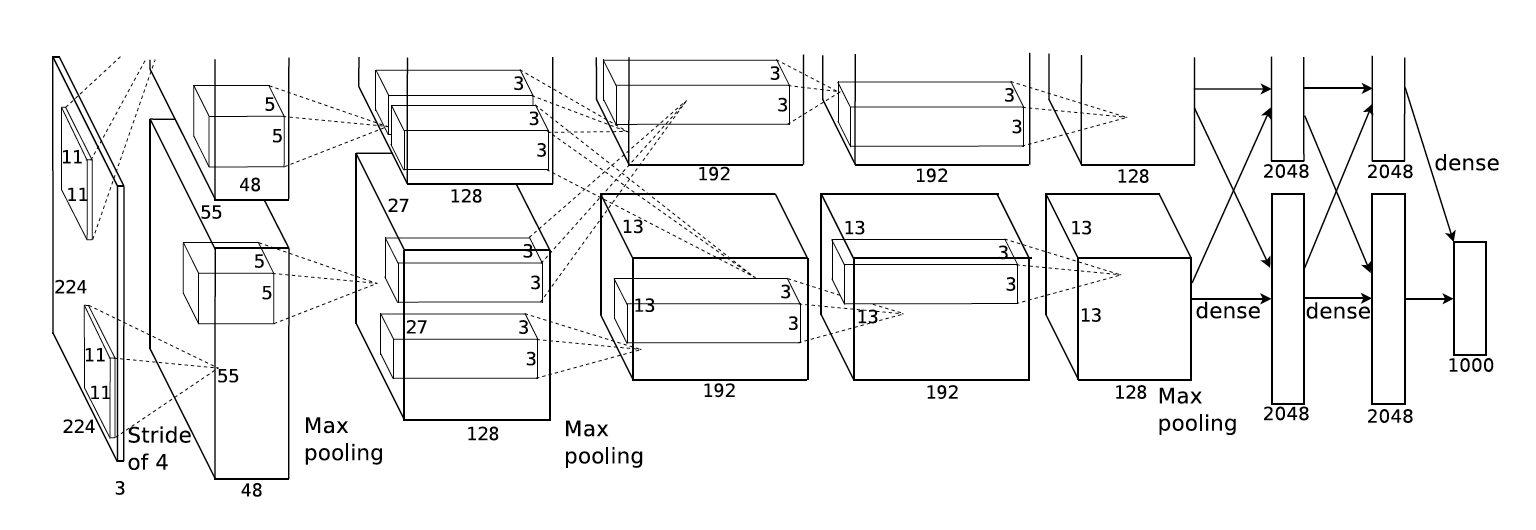
\includegraphics[scale=0.2]{figures/main/ch1-introduction/alexnet.png}
  \caption{The neural network architecture (AlexNet) proposed by~\citet{krizhevsky2012imagenet} which won the ImageNet Large-Scale Visual Recognition Challenge in 2012.}
  \label{figure:ch1-alexnet_network}
\end{figure}

One of the most remarkable breakthroughs of Deep Learning happened in 2012 during the ImageNet Large-Scale Visual Recognition Challenge~\cite{russakovsky2015imagenet}.
The challenge aims at evaluating different algorithms for object detection and image classification.
In 2012, \citeauthor{krizhevsky2012imagenet} obtained \nth{1} place and beat every other participant by a 10.8\% margin with a neural network architecture called \textbf{AlexNet}.
The main reasons for this success are twofold.
First, they used a convolutional neural network (CNN) with more than 60 million parameters which was one of the largest models of the time.
Secondly, they designed a specific architecture to exploit dual programmable graphics processing units (GPUs) to speed up the arithmetic operations, which enabled them to significantly reduce training time.
The \Cref{figure:ch1-alexnet_network} shows the AlexNet architecture which consists of five convolutional layers with two fully connected layers at the end.
The figure also shows the distribution of the workload between the two GPUs.


\begin{table}[t]
  \centering
  \sisetup{
    table-number-alignment = center,
    table-space-text-pre = \ \ \ ,
  }
  \begin{subfigure}[b]{\textwidth}
    \centering
    \begin{tabular}{
      L{5cm}
      L{3.5cm}
      S[table-format=3.0, table-text-alignment=left]@{\,}
      s[table-unit-alignment=left]
      c
    }
      \toprule
      \textbf{Authors} & \textbf{Models} & \multicolumn{2}{c}{\textbf{\#Params}} & \textbf{TOP-5 Acc.} \\
      \midrule
      \citet{krizhevsky2012imagenet} & AlexNet             &  61 & \si{M} & 84.7\% \\
      \citet{simonyan2014very}       & VGG                 & 144 & \si{M} & 92.0\% \\
      \citet{he2016deep}             & ResNet-152          &  60 & \si{M} & 93.8\% \\
      \citet{szegedy2017inception}   & Inception-ResNet-v2 &  56 & \si{M} & 95.1\% \\
      \citet{xie2017aggregated}      & ResNeXt-101         &  84 & \si{M} & 95.6\% \\
      \citet{hu2018squeeze}          & SENet               & 146 & \si{M} & 96.2\% \\
      \citet{real2019regularized}    & AmoebaNet-A         & 469 & \si{M} & 96.7\% \\
      \citet{huang2019gpipe}         & AmoebaNet-B         & 556 & \si{M} & 97.0\% \\
      \bottomrule
    \end{tabular}
    \caption{Computer Vision Models}
    \label{table:ch1-networks_parameters_cv}
  \end{subfigure}
  \par\bigskip
  \begin{subfigure}[b]{\textwidth}
    \centering
    \begin{tabular}{
      L{4.5cm}
      L{4.5cm}
      S[table-format=3.0, table-text-alignment=left]@{\,}
      s[table-unit-alignment=left]
    }
      \toprule
      \textbf{Authors} & \textbf{Models} & \multicolumn{2}{c}{\textbf{\#Params}} \\
      \midrule
      \citet{peters2018deep}         & ELMo            &  94 & \si{M} \\
      \citet{radford2018improving}   & GPT             & 110 & \si{M} \\
      \citet{devlin2019bert}         & BERT            & 340 & \si{M} \\
      \citet{yang2019xlnet}          & XLNet (Large)   & 340 & \si{M} \\
      \citet{liu2019roberta}         & RoBERTa (Large) & 355 & \si{M} \\
      \citet{radford2019language}    & GPT-2           &   1 & \si{B} \\
      \citet{shoeybi2019megatron}    & MegatronLM      &   8 & \si{B} \\
      \citet{raffel2020exploring}    & T5-11B          &  11 & \si{B} \\
      \citet{rosset2020turingnlg}    & T-NLG           &  17 & \si{B} \\
      \citet{brown2020language}      & GPT-3           & 175 & \si{B} \\
      \citet{fedus2021switch}        & Switch Transformers & 1 & \si{T} \\
      \bottomrule
    \end{tabular}
    \caption{Natural Language Processing Models}
    \label{table:ch1-networks_parameters_nlp}
  \end{subfigure}
  \par\bigskip
  \caption{Evolution of the number of parameters for Computer Vision and Natural Language Processing models developed in the years after AlexNet.}
  %   List of Computer Vision and Natural Language Processing models with their number of param
  %   Tables showing the different network architectures developed in the years after AlexNet.
  %   \Cref{table:ch1-networks_parameters_cv} shows networks developed for computer vision tasks and \Cref{table:ch1-networks_parameters_nlp} shows networks developed for natural language processing.
  % }
  \label{table:ch1-networks_parameters}
\end{table}


Following this result, many architectures with an increasing number of parameters have been developed.
This growth in the number of parameters has led to an increase in accuracy, exceeding even human performance, on the ImageNet dataset~\cite{he2015delving}.
\Cref{table:ch1-networks_parameters} shows a list of the different state-of-the-art architectures along with their size and accuracy.
As we can see, the accuracy of the models generally improves at the cost of the model size.
For computer vision models, \citet{tan2019efficientnet} have shown that the relationship between model size and accuracy seems to obey a power law.
% This relationship has also been observed for Natural Language Processing (NLP) neural networks \cite{rosenfeld2020a,kaplan2020scaling} and given the availability of large-scale datasets (Common Crawl dataset~\cite{raffel2019exploring} constitutes nearly a trillion words), researchers have been able to scale their models.
This relationship has also been observed for Natural Language Processing (NLP) neural networks \cite{rosenfeld2020a,kaplan2020scaling} aided by the availability of large-scale datasets such as the Common Crawl dataset~\cite{raffel2019exploring} which constitutes nearly a trillion words.

As a result of their size and improved accuracy, deep neural networks now achieve state-of-the-art performances in a variety of domains such as image recognition~\cite{lecun1998gradient,krizhevsky2012imagenet,he2016deep,tan2019efficientnet}, object detection~\cite{redmon2016you,liu2016ssd,redmon2017yolo9000}, natural language processing~\cite{merity2016pointer,vaswani2017attention,radford2018Language,brown2020language}, speech recognition~\cite{hinton2012deep,abdel2014convolutional,yu2016automatic}, health care \cite{faust2018deep} etc.
Specifically, computer vision and natural language processing models have achieved sufficient performance for being used in real-world applications such as autonomous vehicles~\cite{fagnant2015preparing,sharma2021automating}, translation~\cite{wu2016google}, vocal assistants~\cite{li2017acoustic}, etc.

However, accuracy is not the only concern, when implemented in a critical decision process, neural networks need to be compact, cost-effective and secure.
Although accurate, large neural networks often lack these properties.
Indeed, training state-of-the-art models on computer vision or natural language processing tasks requires gigabytes of memory and can take several months to train on a single GPU~\cite{krizhevsky2012imagenet,brown2020language}.
For example, the GPT-3 model proposed by~\citet{brown2020language}, culminates at 175 billion parameters and requires 355 years of training on a single GPU and \$\numprint{4600000} to train on a cloud-computing platform \cite{li2020overview}.
It has also been estimated by \citet{strubell2019energy} that the training and development costs of the large Transformer model proposed by~\citet{vaswani2017attention} with neural architecture search emits an estimated \numprint{284019} kg of $\mathrm{CO}_2$ whereas a human life will consume an average of \numprint{5000} kg of $\mathrm{CO}_2$ for one year. 
Furthermore, with the rise of smartphones and ``Internet of things'' devices (IoT) with limited computational and memory resources, neural networks also need to be efficient during the inference phase.
In addition, with the growing concern over data privacy, methods such as \emph{federated learning} are gaining ground.
Federated learning involves training a model across multiple decentralized devices (\eg, smartphones) with local data samples.
This avoids the step of centralizing all users' data into one server, thus addressing the issue of data privacy.
Thus, building compact and cost-effective neural networks have been an important goal in order to reduce training time, reduce cost and allow for faster research and development.

In addition to being compact and cost-effective, neural networks also need to be secure.
Due to a high complexity and expressivity, large neural networks exhibit instability to small perturbations of their inputs.
Unstable neural networks tend to be vulnerable to \emph{adversarial examples}, \ie, imperceptible variations of natural examples, crafted to deliberately mislead the models~\cite{globerson2006nightmare,biggio2013evasion,szegedy2013intriguing}.
The \Cref{figure:ch1-adversarial_image_example} gives an example of an adversarial attack on an image.
The small perturbation (center) is added to the original image (left) leading to an adversarial image (right).
This behavior can cause serious security problems when neural networks are used for critical decision-making (\eg, judicial decision, self-driving cars, etc.).

This thesis focuses on the problem of training neural networks which are not only accurate but also compact, easy to train, reliable and robust to adversarial examples.





% The study of security properties of learning algorithms is a research field known as \emph{adversarial machine learning} which dates back to 2004 \cite{dalvi2004adversarial}.
% More recently, the work of \citet{szegedy2013intriguing} has brought considerable attention to adversarial examples in the context of Deep Learning.
% Since then, a number of work has been published in designing attacks and defenses \cite{szegedy2013intriguing,goodfellow2014explaining,papernot2016limitations,madry2018towards,carlini2017towards,pinot2019theoretical}.
% \emph{Adversarial Training} (AT), one of the first effective methods to protect against adversarial examples, was introduced by \citet{goodfellow2014explaining} and later improved by \citet{madry2018towards}.
% It consists of augmenting training batches with adversarial examples generated during the training procedure.
% More recently, a new method \cite{farnia2018generalizable} based on the regularization of the Lipschitz constant of the network has been proposed which linked the generalization capabilities of neural networks to their Lipschitz constant; therefore, a reduced Lipschitz constant could lead to a better generalization.
% Although these methods improve the robustness of neural networks, the accuracy obtained ``under attack'' is far from state-of-the-art and therefore security risks are still present.
%






%%%%%%%%%%%%%%%%%%%%%%%%%%%%%%%%%%%%%%%%%%%%%%%%%%%%%%%%%%%%%%%%%%%%%%%%%%%%%%%
\section{Problem Statement and Contributions}
\label{section:ch1-problem_statement_and_contributions}
%%%%%%%%%%%%%%%%%%%%%%%%%%%%%%%%%%%%%%%%%%%%%%%%%%%%%%%%%%%%%%%%%%%%%%%%%%%%%%%


\begin{figure}[t]
   \centering
   \begin{subfigure}[t]{0.24\textwidth}
       \centering
       \begin{equation*}
	  \leftmatrix
	    a &   &   &   \\
	      & b &   &   \\
	      &   & c &   \\
	      &   &   & d
	  \rightmatrix
       \end{equation*}
       \caption*{diagonal}
   \end{subfigure}
   \hfill
   \begin{subfigure}[t]{0.24\textwidth}
       \centering
       \begin{equation*}
	  \leftmatrix
	    a & b & c & d \\
	    e & a & b & c \\
	    f & e & a & b \\
	    d & f & e & a
	  \rightmatrix
       \end{equation*}
       \caption*{Toeplitz}
   \end{subfigure}
   \hfill
   \begin{subfigure}[t]{0.24\textwidth}
       \centering
       \begin{equation*}
	  \leftmatrix
	    ae & af & ag & ah \\
	    be & bf & bg & bh \\
	    ce & cf & cg & ch \\
	    de & df & dg & dh
	  \rightmatrix
       \end{equation*}
       \caption*{Low Rank}
   \end{subfigure}
   \hfill
   \begin{subfigure}[t]{0.24\textwidth}
       \centering
       \begin{equation*}
	  \leftmatrix
	    a & a^2 & a^3 & a^4 \\
	    b & b^2 & b^3 & b^4 \\
	    c & c^2 & c^3 & c^4 \\
	    d & d^2 & d^3 & d^4
	  \rightmatrix
       \end{equation*}
       \caption*{Vandermonde}
   \end{subfigure}
  \caption{Examples of structured matrices.}
  \label{figure:ch1-example_structure_matrices}
\end{figure}


Neural networks, which find their roots in the work of \citet{mcculloch1943logical,rosenblatt1958perceptron}, can be analytically described as a composition of multi-dimensional linear functions interlaced with nonlinear functions (also called activation functions).
More formally, a neural network is a function $N_{\Omega} : \Rbb^n \rightarrow \Rbb^m$ parameterized by a set of weights $\Omega$ of the form:
\begin{equation} \label{equation:ch1-neural_network}
  N_{\Omega}(\xvec) = \psi^{(\depth)} \circ \rho \circ \psi^{(\depth-1)} \cdots \circ \psi^{(2)} \circ \rho \circ \psi^{(1)} (\xvec) \enspace.
\end{equation}
Here, $\depth$ corresponds to the \emph{depth} of the network (\ie, the number of layers) and $\rho$ is a nonlinear function.
Finally, each $\psi^{(i)}$ is a multi-dimensional linear function $\psi^{(i)}: \xvec \mapsto \Wmat^{(i)} \xvec + \bvec^{(i)}$ parameterized by a weight matrix $\Wmat^{(i)}$ and a bias vector $\bvec^{(i)}$ and $\Omega$ is the union of the parameters of each layer. 
% (we present a more formal definition of neural networks in~\Cref{chapter:ch2-background}). 


Classical neural networks typically have a large number of parameters to train.
% For example, a two-layer \emph{fully connected neural networks}, networks in which all the neurons from one activation are connected to all the neurons of the following activation -- \ie, meaning the weight matrix of each layer is \emph{dense} -- will have a minimum of $n \times m + m^2$ parameters where $n$ is the size of the input and $m$ is the size of the output (number of classes).
% The dimension of the input is usually large, for example, with the ImageNet dataset $n = 224^2 \times 3$ and $m = 1000$ leading to a two-layer fully connected neural network with more than 150 million parameters.
If they have no restrictions on the weight matrices $\Wmat^{(i)}$, the layers are said to be \emph{fully connected}.
Typically, fully connected neural networks have a large number of parameters.
For example, a fully connected neural network with $\depth$ layers and $n$ neurons on each layer ($\Wmat^{(i)} \in \Rbb^{n \times n}$) will have $\bigO\left(pn (n + 1)\right)$ parameters.
Since the input and output dimensions are generally large (\eg, ImageNet has an input dimension of $224^2 \times 3$ and an output of 1000), simple fully connected neural networks with few layers accumulate over hundreds of millions of parameters.
Generally, this type of neural network has been shown to perform poorly due to a large search space.
Moreover, they are computationally expensive, which makes them impractical for a number of use cases (smartphones, IoT devices, etc.).
To reduce the number of parameters on each layer, researchers have devised specific linear operations that reduce the number of parameters and have better properties for the problem at hand.


\begin{figure}[t]
  \centering
  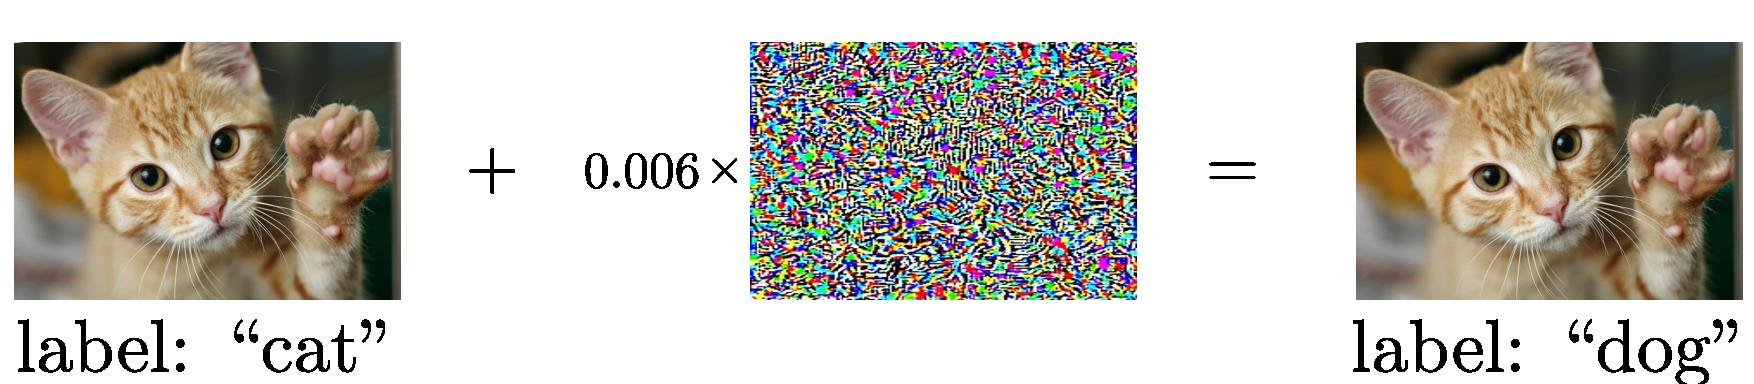
\includegraphics[width=\textwidth]{figures/main/ch1-introduction/ExampleAdversarialCatDog.pdf}
  \caption{Example of Adversarial Attack on an image.}
  \label{figure:ch1-adversarial_image_example}
\end{figure}

An example of widely used neural networks with specialized and more compact linear operations are \emph{Convolutional Neural Networks} (CNN)~\cite{lecun1998gradient,krizhevsky2012imagenet,he2016deep,tan2019efficientnet} which achieve state-of-the-art results for computer vision tasks.
Convolutional neural networks use specific weight matrices which encode the translation invariant property often desirable to process images.
% They use convolutional layers which are specific to image processing and use very few parameters.
Whereas a classical linear layer with a dense matrix will have $n \times n$ parameters, a convolution layer only has $k \times k$ parameters where $k \ll n$ is the kernel size and is usually small (\eg, 3 or 5 for classical convolutional layers).
A convolutional neural network is the most common type of \emph{structured} neural network.
Indeed, the convolution operation can be represented by a structured matrix \ie, a matrix that can be represented with less than $n^2$ parameters.


In addition to offering a more compact representation, the structure of certain matrices can be exploited to obtain better algorithms for the matrix-vector product, thus optimizing memory and computing operations.
Based on the success of convolutional neural networks, researchers have studied and proposed other types of neural networks based on weight matrices with different structures~\cite{moczulski2016acdc,sindhwani2015structured}.
\Cref{figure:ch1-example_structure_matrices} shows different types of structured matrices that have been used for deep learning.
Although convolutional neural networks have been state-of-the-art for computer vision tasks, it remains unclear whether other types of structured neural networks can be beneficial to other types of applications and which type of structure can provide both accuracy and efficient computation.

The contributions of this thesis lie at the intersection of linear algebra, Fourier analysis and deep learning.
As a result, we build compact and secure neural networks by leveraging the properties of structured matrices from the Toeplitz family.
Hereafter, we detail our contributions.

%%%%%%%%%%%%%%%%%%%%%%%%%%%%%%%%%%%%%%%%%%%%%%%%%%%%%%%%%%%%%%%%%%%%%%%%%%%%%%%%
\subsection{Training Compact Neural Networks}
\label{subsection:ch1-training_compact_neural_networks}
%%%%%%%%%%%%%%%%%%%%%%%%%%%%%%%%%%%%%%%%%%%%%%%%%%%%%%%%%%%%%%%%%%%%%%%%%%%%%%%%


% In addition, neural networks with a smaller number of parameters generalize better.
% This phenomenon has been theoretically justified by \citet{vapnik1982estimation}.
% Indeed, \citeauthor{vapnik1982estimation} linked the generalization capability of neural networks to their VC-dimension which is a measure of expressivity of the class of functions.
% This complexity measure is based on the number of parameters, therefore, reducing the number of parameters leads to a smaller VC-Dimension, which then leads to better generalization.

As a first contribution, we use circulant matrices, which are a particular type of Toeplitz matrix, to devise a new compact architecture replacing fully connected neural networks.
More precisely, we study deep diagonal-circulant neural networks, which are deep neural networks in which weight matrices are the product of diagonal and circulant ones.
Besides making a theoretical analysis of their expressivity, we introduce principled techniques for training these models: we devise an initialization scheme and propose a smart use of nonlinearity functions in order to train deep diagonal circulant networks.
Furthermore, we show that these networks outperform recently introduced deep networks with other types of structured layers.
We conduct a thorough experimental study to compare the performance of deep diagonal circulant networks with state-of-the-art models. 
%based on structured matrices and with dense models.
We show that our models achieve better accuracy than other structured approaches while requiring 2x fewer weights than the next best approach.
Finally, we train accurate deep diagonal circulant networks on a real-world video classification dataset with over 3.8 million training examples.
% Finally, we train deep diagonal circulant networks on a real-world video classification dataset with over 3.8 million training examples.

The training procedure we have developed to train large diagonal-circulant neural networks was first published in the \textbf{\color{mydarkblue} European Conference on Computer Vision Workshops on Video Classification}, as part of the \yt challenge.
Then, the theoretical analysis of the expressivity of diagonal-circulant neural networks has been published in a second paper in the \textbf{\color{mydarkblue} 24th European Conference on Artificial Intelligence}.



%%%%%%%%%%%%%%%%%%%%%%%%%%%%%%%%%%%%%%%%%%%%%%%%%%%%%%%%%%%%%%%%%%%%%%%%%%%%%%%%
\subsection{Training Robust Neural Networks}
\label{subsection:ch1-training_robust_neural_networks}
%%%%%%%%%%%%%%%%%%%%%%%%%%%%%%%%%%%%%%%%%%%%%%%%%%%%%%%%%%%%%%%%%%%%%%%%%%%%%%%%

As a second contribution, we build robust neural networks by studying the properties of the structure of convolutions.
We devise a new upper bound on the largest singular value of convolution layers that is both tight and easy to compute.
Our work is based on the result of~\citet{gray2006toeplitz} which states that an upper bound on the singular value of Toeplitz matrices can be computed from the inverse Fourier transform of the characteristic sequence of these matrices.
From our analysis immediately follows an algorithm for bounding the Lipschitz constant of a convolutional layer, and by extension the Lipschitz constant of the whole network.
Finally, we illustrate our approach to adversarial robustness.
Recent work has shown that empirical methods such as adversarial training offer poor generalization~\cite{schmidt2018adversarially} and can be improved by applying Lipschitz regularization~\cite{farnia2018generalizable}.
To illustrate the benefit of our new method, we train neural networks with Lipschitz regularization and show that it offers a significant improvement over adversarial training alone.

The main result of the work described in \Cref{chapter:ch5-lipschitz_bound} has been published in the \textbf{\color{mydarkblue}\nth{35} AAAI Conference on Artificial Intelligence}.
Additional joint contributions have also been published on the topic of robust neural networks.
The first work, published in the \textbf{\color{mydarkblue} Advances in Neural Information Processing Systems}, studies the effectiveness of noise injection at training and inference time in the network to protect against adversarial attacks.
In this work, we show that noise drawn from the Exponential family offers a provable protection against adversarial attacks. 
The second joint contribution, published in the \textbf{\color{mydarkblue} European Conference on Machine Learning Workshop for CyberSecurity}, conducts a geometrical analysis of defense mechanisms designed to protect neural networks against.
This work shows that neural networks designed to be robust against one type of adversarial example offer poor against other types of attacks.





% In this thesis, we study the properties of structured matrices from the Toeplitz family and make contributions to the field of supervised learning with neural networks.
% This thesis is organized in two parts.
% First, we use circulant matrices, which are a particular case of Toeplitz matrices, to devise a new compact architecture replacing Fully Connected Neural Networks.
% More precisely, we study deep diagonal-circulant neural networks, which are deep neural networks in which weight matrices are the product of diagonal and circulant ones.
% Besides making a theoretical analysis of their expressivity, we introduce principled techniques for training these models: we devise an initialization scheme and propose a smart use of nonlinearity functions in order to train deep diagonal circulant networks.
% Furthermore, we show that these networks outperform recently introduced deep networks with other types of structured layers.
% We conduct a thorough experimental study to compare the performance of deep diagonal circulant networks with state-of-the-art models based on structured matrices and with dense models.
% We show that our models achieve better accuracy than other structured approaches while requiring 2x fewer weights than the next best approach.
% Finally, we train compact and accurate deep diagonal circulant networks on a real-world video classification dataset with over 3.8 million training examples.
% In the second part of this thesis, we study the properties of the structure of convolution to devise a new upper bound on the largest singular value of convolution layers that is both tight and easy to compute.
% Our work is based on the result of~\citet{gray2006toeplitz} which states that an upper bound on the singular value of Toeplitz matrices can be computed from the inverse Fourier transform of the characteristic sequence of these matrices.
% From our analysis immediately follows an algorithm for bounding the Lipschitz constant of a convolutional layer, and by extension the Lipschitz constant of the whole network.
% Finally, we illustrate our approach on adversarial robustness.
% Recent work has shown that empirical methods such as adversarial training (AT) offer poor generalization~\cite{schmidt2018adversarially}, and can be improved by applying Lipschitz regularization~\cite{farnia2018generalizable}.
% To illustrate the benefit of our new method, we train neural networks with Lipschitz regularization and show that it offers a significant improvement over adversarial training alone.


%%%%%%%%%%%%%%%%%%%%%%%%%%%%%%%%%%%%%%%%%%%%%%%%%%%%%%%%%%%%%%%%%%%%%%%%%%%%%%%
\section*{Outline of the Thesis}
\label{section:ch1-outline_of_the_thesis}
%%%%%%%%%%%%%%%%%%%%%%%%%%%%%%%%%%%%%%%%%%%%%%%%%%%%%%%%%%%%%%%%%%%%%%%%%%%%%%%

This thesis is organized in six chapters.
First, \Cref{chapter:ch2-background} gives an introduction to the theory of Toeplitz matrices and on supervised learning and neural networks.
This chapter presents the necessary technical tools we will need for presenting the related work and for our contributions.
\Cref{chapter:ch3-related_work} is dedicated to enumerating the state-of-the-art approaches.
The chapter is divided into two parts.
First, we review techniques to build compact neural networks with an important focus on techniques that use structured matrices.
The second part focuses on presenting regularization methods for improving the robustness of neural networks.
\Cref{chapter:ch4-diagonal_circulant_neural_network} and \Cref{chapter:ch5-lipschitz_bound} constitute our main contributions.
\Cref{chapter:ch4-diagonal_circulant_neural_network} presents results on compact neural networks built from diagonal and circulant matrices.
\Cref{chapter:ch5-lipschitz_bound} presents our new regularization scheme to improve the robustness of neural networks based on the properties of doubly-block Toeplitz matrices.
\Cref{chapter:ch6-conclusion} proposed a discussion and some perspectives on the contributions.
Appendix~\ref{appendix:ap2-diagonal_circulant_neural_networks_for_video_classification} constitutes some complements to~\Cref{chapter:ch4-diagonal_circulant_neural_network}.
It provides additional experiments on video classification with compact neural networks.
Finally, Appendix~\ref{appendix:ap3-theoretical_evidence_for_adversarial_robustness_through_randomization} and Appendix~\ref{appendix:ap4-advocating_multiple_defense_strategies_against_adversarial_examples} provide further work on the robustness of neural networks done during this Ph.D. thesis.
% Finally, Appendix~\ref{appendix:ap6-publications} enumerates the publications made during this Ph.D. thesis.





  %%%%%%%%%%%%%%%%%%%%%%%%%%%%%%%%%%%%%%%%%%%%%%%%%%%%%%%%%%%%%%%%%%%%%%%%
\chapter{Background}
\label{chapter:ch2-background}
%%%%%%%%%%%%%%%%%%%%%%%%%%%%%%%%%%%%%%%%%%%%%%%%%%%%%%%%%%%%%%%%%%%%%%%%
\localtoc

This chapter gives a short introduction on the theory of supervised learning~\cite{shalev2014understanding} and Toeplitz matrices~\cite{gray2006toeplitz}.
In the statistical learning framework, supervised learning refers to the problem of optimizing the parameters of a function in order to map an input to an output based on a series of input-output pairs.
For example, an image (input) mapped to a class (output) describing its content.
The first section describes a formal model that aims to describe such learning tasks.
In linear algebra, a Toeplitz matrix, named after Otto Toeplitz, is a matrix in which each descending diagonal, from left to right, is constant.
The second section describes the mathematical properties of Toeplitz matrices and known theorems that we use in this thesis. 


%%%%%%%%%%%%%%%%%%%%%%%%%%%%%%%%%%%%%%%%%%%%%%%%%%%%%%%%%%%%%%%%%%%%%%%%%%%%%%%
\section{Introduction on Supervised Learning}
\label{section:ch2-introduction_on_supervised_learning}
%%%%%%%%%%%%%%%%%%%%%%%%%%%%%%%%%%%%%%%%%%%%%%%%%%%%%%%%%%%%%%%%%%%%%%%%%%%%%%%

\begin{figure}[t]
  \centering
  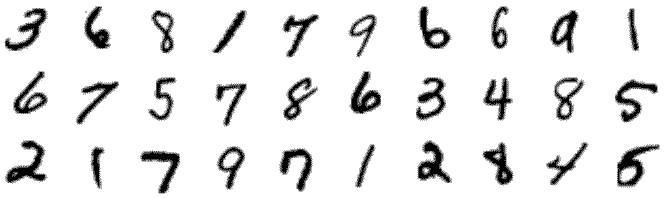
\includegraphics[width=0.85\textwidth]{figures/main/ch2-background/mnist-dataset.png}
  \caption{Images with handwritten digits in the MNIST database \cite{lecun1998gradient}}
  \label{figure:ch2-mnist-database}
\end{figure}


In \citeyear{lecun1998gradient}, \citeauthor{lecun1998gradient} had successfully learned a function capable of recognizing handwritten digits in images.
They used the MNIST database \cite{lecun1998gradient} which consists of black and white images of size $28 \times 28$ pixels (see \Cref{figure:ch2-mnist-database}).
Their goal was to build a machine that takes a vector as input and produces the identity of the digit $0 \dots 9$ as the output.
This is a non-trivial problem because each image is unique and while digits can be differentiated based on their shapes and strokes, these features give poor results for an automated system. 

In the following, we will formalize the learning problem describe above with the \emph{statistical learning framework}.
First, let us define the domain space $\mathcal{X}$ which corresponds to the set of images that we wish to label.
In our example above, this domain corresponds to the set of all possible images with handwritten digits.
Let us denote the label space $\mathcal{Y}$ and a finite sequence of pairs $\mathcal{S} = \left\{ \left(\xvec^{(1)}, y^{(1)} \right) \dots \left( \xvec^{(m)}, y^{(m)} \right) \right\}$ in $\mathcal{X} \times \mathcal{Y}$. 
Such pairs \ie, labeled examples, are called \emph{training examples} and the set $\mathcal{S}$ is called the \emph{training set}.
We denote $\mathcal{D}$ the \emph{joint distribution} over $\mathcal{X} \times \mathcal{Y}$.
The main objective of the task at hand is to output a \emph{prediction rule} $h: \mathcal{X} \rightarrow \mathcal{Y}$ that maps the input $\xvec \in \mathcal{X}$ to the output $y \in \mathcal{Y}$.
This function is called the \emph{hypothesis} or the \emph{classifier}. 
Given the probability distribution $\mathcal{D}$, we aim to measure how \emph{likely} the hypothesis $h$ makes an error when labeled points are randomly drawn from the distribution $\mathcal{D}$.
Let us define the true error or \emph{risk} of the hypothesis $h$ that we which to minimize:
\begin{equation}
  R_{\mathcal{D}}(h) \triangleq \Pbb_{(\xvec, y) \sim \mathcal{D}} \left[ h(\xvec) \neq  y \right] \enspace.
  \label{equation:ch2-risk1}
\end{equation}
However, in practice, the joint probability distribution $\mathcal{D}$ is unknown; therefore, the true error is not directly available to the learner.
The learner only has access to the training data, $\mathcal{S}$, and can calculate the \emph{empirical error} \ie, the error over the training samples.
We define the \emph{empirical risk} as follows:
\begin{equation}
  R_{\mathcal{S}}(h) \triangleq \frac{\left| \left\{i \in [m]: h\left(\xvec^{(i)}\right) \neq y^{(i)} \right\}\right|}{m} \enspace.
\end{equation}
We can generalize our measure of correctness so that it can be applied to multiple learning tasks.
Let us define a \emph{loss function} from $\mathcal{Y} \times \mathcal{Y}$ to the set of nonnegative real numbers, $L: \mathcal{Y} \times \mathcal{Y} \rightarrow \Rbb_{+}$.
We can express the \emph{risk} as follows:
\begin{equation}
  R_{\mathcal{D}}(h) \triangleq \Ebb_{(\xvec, y) \sim \mathcal{D}} \left[ L\big( h(\xvec), y \big) \right] \enspace.
  \label{equation:ch2-risk2}
\end{equation}
Similarly, we express the empirical risk as follows:
\begin{equation}
  R_{\mathcal{S}}(h) \triangleq \frac{1}{m} \sum_{(\xvec, y) \sim \mathcal{S}} L\big( h(\xvec), y \big) \enspace.
\end{equation}
The loss functions used for classification problems and regression problems are as follows: 
\begin{itemize}
  \item \textbf{0-1 Loss}: $L_{0-1}\big( h(\xvec), y \big) = \mathds{1}\big[ h(\xvec) \neq y \big]$ \\
  This loss is used for classification problems, for example, when the learner have to recognizing hand-written digits in images.
  We can notice that the definitions of $R_{\mathcal{D}}$ given in \Cref{equation:ch2-risk1} and \Cref{equation:ch2-risk2} coincide.
  \item \textbf{Square Loss}: $L_{\text{sq}} \big( h(\xvec), y \big) = \big( h(\xvec) - y \big)^2$ \\	
  This loss is used for another common type of learning problem \ie, \emph{regression problem}, in which the label domain $\mathcal{Y}$ is the set of real numbers.
  For example, one wishes to predict the price of an apartment given its characteristics.
\end{itemize}


The goal of the learning algorithm is to find the hypothesis $h$ that minimize the risk $R_{\mathcal{S}}$, this learning paradigm is called \emph{Empirical Risk Minimization} (ERM).
We use the ERM paradigm as a surrogate to find a hypothesis $h$ that minimize the true risk $R_\mathcal{D}$.
However, all hypothesis that minimize the empirical error does not necessarily minimize the true risk.
For example, consider the following function:
\begin{equation}
  h^*(\xvec) =
  \begin{cases}
    y^{(i)} &\quad \text{if }\exists i \in [m] \text{ s.t. } \xvec^{(i)} = \xvec \\
    0 &\quad \text{otherwise}
  \end{cases}
  \label{equation:ch2-perfect_function}
\end{equation}
Clearly, this function, for any training set, $\mathcal{S}$, will have $R_\mathcal{S}(h^*) = 0$, whereas the true risk would certainly be high.
The phenomenon, called \emph{overfitting}, happens when the classifier fits the training data ``too well'' but will likely have a high error on unseen data.
One possible solution to this phenomenon is to apply ERM with a restricted search space to prevent the learning algorithm to output a function such as $h^*$ in \Cref{equation:ch2-perfect_function}.
We call this set the \emph{hypothesis class} and is denoted $\mathcal{H}$. 
Each $h \in \mathcal{H}$ is a function mapping from $\mathcal{X}$ to $\mathcal{Y}$.
We call $\mathrm{ERM}_{\mathcal{H}}$, the learned that use the $\mathrm{ERM}$ paradigm over the hypothesis class $\mathcal{H}$ and a training data $\mathcal{S}$.
Formally,
\begin{equation}
  \mathrm{ERM}_{\mathcal{H}}(\mathcal{S}) \in \argmin_{h \in \mathcal{H}} R_{\mathcal{S}}(h) \enspace.
\end{equation}
For a training sample $\mathcal{S}$, we denote $h_\mathcal{S}$, one solution of applying $\text{ERM}_\mathcal{H}$ on the set $\mathcal{S}$, if there exists multiple hypotheses with minimal error on the training sample, then minimization problem returns an arbitrary one.
In practice, the hypothesis class is chosen based on a hypothesis on the relation between the data and its label.
For example, if the relation between the data and its label is supposedly linear then the hypothesis class can be the set of all linear function.
This kind of restriction is called an \emph{inductive bias} because the learner is \emph{biased} toward a particular set of predictors.

\begin{figure}[t]
  \centering
  \begin{subfigure}[b]{0.32\textwidth}
    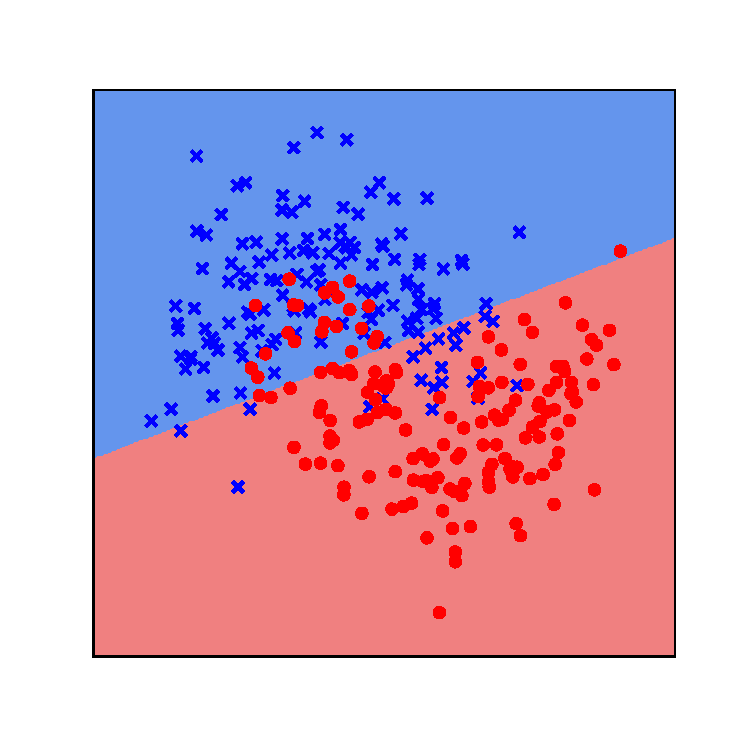
\includegraphics[width=0.98\textwidth]{figures/main/ch2-background/underfitting.pdf}
    \caption{Underfitting}
    \label{figure:ch2-fitting_points_a}
  \end{subfigure}
  \hfill
  \begin{subfigure}[b]{0.32\textwidth}
    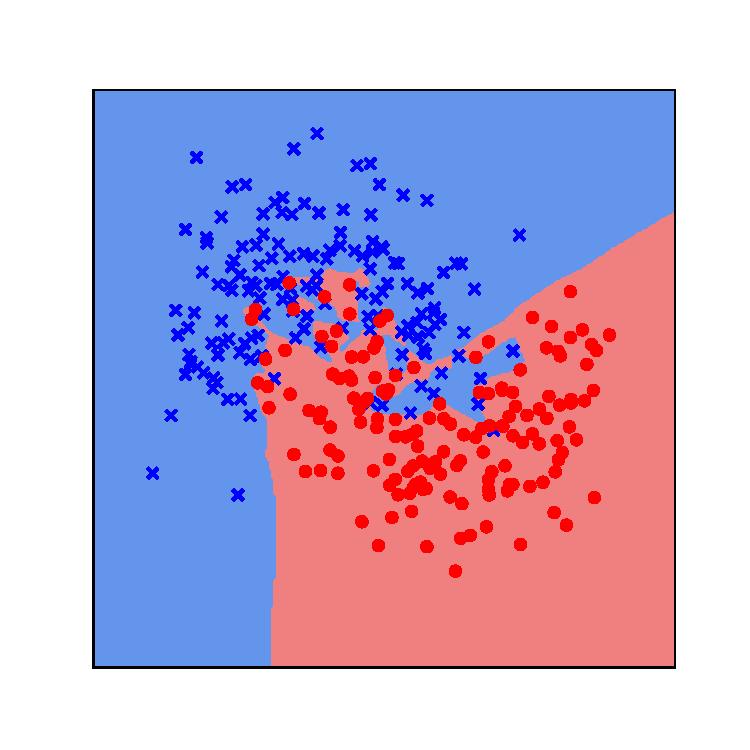
\includegraphics[width=0.98\textwidth]{figures/main/ch2-background/overfitting.pdf}
    \caption{Overfitting}
    \label{figure:ch2-fitting_points_b}
  \end{subfigure}
  \hfill
  \begin{subfigure}[b]{0.32\textwidth}
    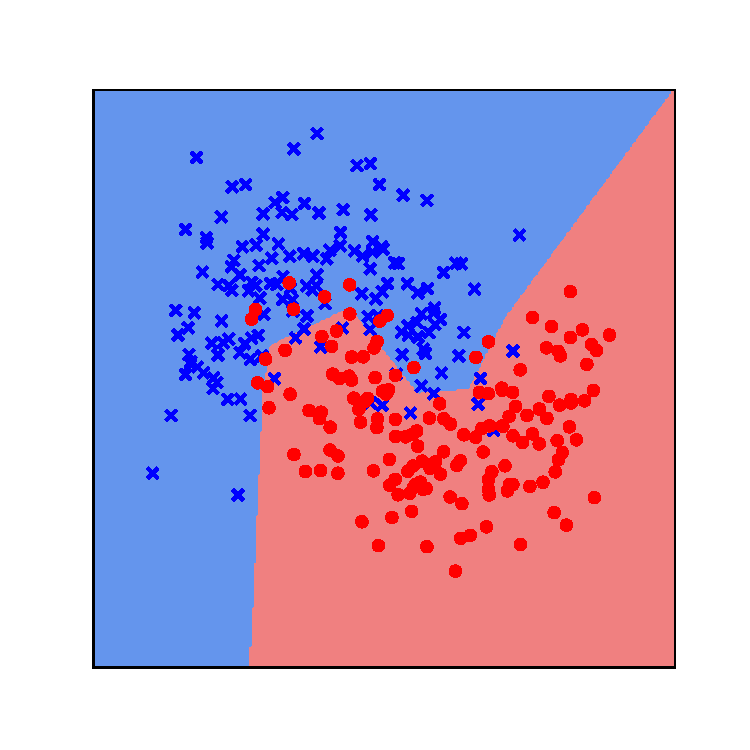
\includegraphics[width=0.98\textwidth]{figures/main/ch2-background/normal.pdf}
    \caption{Good fit}
    \label{figure:ch2-fitting_points_c}
  \end{subfigure}
  \caption{
    Decision boundary of 3 classifiers with different complexity for the same set of sample.
  }
  \label{figure:ch2-fitting_points}
\end{figure}


A fundamental question remains: \emph{how to choose the correct hypothesis class for which $\text{ERM}_\mathcal{H}$ will not lead to overfitting?} 
We answer this question by decomposing the true risk into two different components as follows: 
\begin{equation}
  R_\mathcal{D} (h_\mathcal{S}) = 
  \underbrace{\left[ \min_{h \in \mathcal{H}} R_\mathcal{D}(h) \right]}_{\text{\scriptsize Approximation Error}} + \quad 
  \underbrace{\left[ R_\mathcal{D}(h_\mathcal{S}) - \min_{h \in \mathcal{H}} R_\mathcal{D}(h) \right]}_{\text{\scriptsize Estimation Error}} 
  \label{equation:ch2-bias_complexity_tradeoff}
\end{equation}
\begin{itemize}
  \item \textbf{Approximation Error}: The approximation error corresponds to the minimum risk achievable by a classifier in the given hypothesis class.
  Intuitively, this error measure the quality of the hypothesis class and therefore the quality of the prior knowledge.
  Enlarging the hypothesis class, \ie, allowing more complex functions, can decrease the approximation error.
  \item \textbf{Estimation Error}: The estimation error is the difference between the approximation error and the error made by the ERM predictor.
  Recall that the empirical risk is only an estimate of the true risk.
  This error is dependent on the sample size and/or the complexity of the hypothesis class. 
\end{itemize}
Recall that the main goal is to minimize the true risk $R_\mathcal{D} (h_\mathcal{S})$, however, \Cref{equation:ch2-bias_complexity_tradeoff} shows a tradeoff called the \emph{bias-complexity tradeoff}.
The tradeoff is as follows: if we choose a large and complex hypothesis space, we reduce the approximation error but at the same time can increase the estimation error because a complex hypothesis space might lead to overfitting.
Conversely, choosing a small hypothesis space might reduce the estimation error but increase the approximation error leading to an \emph{underfitting} phenomenon.
We can demonstrate the \emph{overfitting} and \emph{underfitting} phenomenons with \Cref{figure:ch2-fitting_points} which shows the decision boundary of 3 classifiers for the same set of samples.
\Cref{figure:ch2-fitting_points_a} shows a classifier which \emph{underfit} the data, meaning the decision boundary is not complex enough to separate the data correctly.
The \Cref{figure:ch2-fitting_points_b} shows a classifier that almost perfectly follows the training data but is likely to have a higher error rate on the unseen data.
Finally, the \Cref{figure:ch2-fitting_points_c} shows a classifier that seems to have a good compromise between the two.

As seen above, defining a small hypothesis class might lead to underfitting and a large hypothesis class might lead to overfitting.
A good way to offset a large hypothesis class would be to specific preference over hypothesis within the hypothesis class.
The \emph{Structural Minimization Paradigm} (SRM) assumes that the hypothesis class can be written as the union of multitude smaller hypothesis class as follows: $\mathcal{H} = \bigcup_{n \in \Nbb} \mathcal{H}_n$ with a weight function $w: \Nbb \rightarrow [0, 1]$ which assigns a weight to each hypothesis class, $\mathcal{H}_n$, such that a higher weights reflects a lower preference for the hypothesis class.
Intuitively, the weight function is a measure of the ``complexity'' of the hypotesis.
The SRM learning paradigm can then be defined as follows:
\begin{equation}
  \text{SRM}_\mathcal{H} \in \argmin_{h \in \mathcal{H}, n \in \Nbb} \left[ R_\mathcal{S}(h) + w(n) \right]
\end{equation}
The SRM learning paradigm minimizes the empirical risk $R_\mathcal{S}(h)$ and the weight function $w$; therefore, ovoiding overfitting and improving generalization by reducing the complexity of the hypotesis while maintening a low empirical risk. 
% In the next section, we will present neural networks which are the type of function we will use as predictors and we will see how to implement the ERM and SRM paradigm.









% \‰\‰\‰
%
% The ERM paradigm with inductive bias is based on an important assumption.
% We assume that uniformly over all $h \in \mathcal{H}$, the empirical risk is close to the true risk, meaning, an $h$ that minimize the empirical risk with respect to a data set $\mathcal{S}$ will also minimize the \emph{true} risk.
% More formally, 
% \begin{equation}
%   \forall h \in \mathcal{H}, \quad \left| R_\mathcal{S}(h) - R_\mathcal{D}(h) \right| \leq \epsilon \enspace.
%   \label{equation:ch2-eps_respresentative_sample} 
% \end{equation}
% If this assumption is met, then the ERM paradigm will always return a good classifier. 
% \begin{lemma}[Lemma 4.2 \citet{shalev2014understanding}] 
%   If \Cref{equation:ch2-eps_respresentative_sample} hold, then any output of $\mathrm{ERM}_\mathcal{H}(\mathcal{S})$, namely, any $h_\mathcal{S} \in \argmin_{h \in \mathcal{H}} R_\mathcal{S}(h)$, satisfies
%   \begin{equation}
%     R_\mathcal{D}(h_\mathcal{S}) \leq \min_{h \in \mathcal{H}} R_\mathcal{S}(h) + 2\epsilon
%   \end{equation}
% \end{lemma}
%
% \‰\‰\‰


% Let us consider an input space $\mathcal{X} = [0, 1]^d$ of dimension $d$, an output space $\mathcal{Y} = [k]$ where $k$ is the number of class and a data distribution $\mathcal{D}$ over $\mathcal{X} \times \mathcal{Y}$.
% We seek to find a function $h: \mathcal{X} \rightarrow \mathcal{Y}$ that maps the input $\xvec \in \mathcal{X}$ to the output $y \in \mathcal{Y}$ with $h \in \mathcal{H}$ where $h$ is called the \emph{hypothesis} and $\mathcal{H}$ the \emph{hypothesis space}.
% in order to measure how well the function fits, we de\emph{loss function} $l: \mathcal{y} \times \mathcal{y} \rightarrow \rbb^{+}$ is defined.
% The \emph{risk} $R$ associated with the hypothesis $h(\xvec)$ is defined as follows:
% \begin{equation}
%   R(h) \triangleq \Ebb_{(\xvec, y) \sim \mathcal{D}}\  L \left( h(\xvec), y \right)
% \end{equation}
% The goal of a \emph{learning algorithm} is to find a hypothesis $h^* \in \mathcal{H}$ which minimize the risk $R(h)$:
% \begin{equation}
%   h^* \triangleq \argmin_{h \in \mathcal{H}} R(h) .
% \end{equation}

% In practice, the joint probability distribution $\mathcal{D}$ is unknown.
% Instead, we have $n$ independent observations of the distribution called the \emph{training set}
% \begin{equation}
%   \mathcal{T} \triangleq \left\{ \left(\xvec^{(1)}, y^{(1)} \right), \dots, \left( \xvec^{(n)}, y^{(n)} \right) \right\} ,
% \end{equation}
% where $\xvec \in \mathcal{X}$ and $y \in \mathcal{Y}$.

% The risk minimization problem is therefore replace by the \emph{empirical risk minimization} as follows:
% \begin{equation}
%   E(h, n) \triangleq \frac{1}{n} \sum_{i = 1}^{n} L\left(h\left(\xvec^{(i)}\right), y^{(i)}\right) ,
% \end{equation}
% the learning algorithm then becomes:
% \begin{equation}
%   \hat{h}^* \triangleq \argmin_{h \in \mathcal{H}} E(h, n)  .
% \end{equation}


% \paragraph{Structural Risk Minimization} (SRM).
% The ERM principle assumes that the function $\hat{h}^*$ minimizing $E(h, n)$ leads to the risk $R(\hat{h}^*)$ being close to the minimum.
% This assumption mean that as the \emph{size} of the training set increase the minimization becomes more accurate. More formally, the ERM principle assumes that $R(\hat{h}^*)$ converge to its minimum value on the set $h \in \mathcal{H}$ when $n \rightarrow \infty$.  
% \citet{Vapnik1991TheNA} have shown that this equivalent to say that the empirical risk $E(h, n)$ \emph{converge uniformly} to the actual risk $R(h)$ over $h \in \mathcal{H}$ where the \emph{uniform convergence} is defined as follows:
% \begin{equation}
%   \Pbb \left[ \sup_{h \in \mathcal{H}} \left| R(h) - E(h, n) \right| < \epsilon \right] \rightarrow 0 \quad \text{ when } \quad n \rightarrow \infty, \quad \forall \epsilon > 0 
% \end{equation}


% \citet{Vapnik1991TheNA} have shown that this assumption is equivalent to the following: does the empirical risk $E(h, n)$ \emph{converge uniformly} to the actual risk $R(h)$ over $h \in \mathcal{H}$ where the \emph{uniform convergence} is defined as follows:
% \begin{equation}
%   \Pbb \left[ \sup_{h \in \mathcal{H}} \left| R(h) - E(h, n) \right| < \epsilon \right] \rightarrow 0 \quad \text{ when } \quad n \rightarrow \infty, \quad \forall \epsilon > 0 
% \end{equation}


% However, does increasing the \emph{size} of the training set allow a better minimisation of the actual risk. More formally, does $R(\hat{h}^*)$ converge to its minimum value on the set $h \in \mathcal{H}$ when $n \rightarrow \infty$. 

% \citet{vapnik1992principles} 

% The 0-1 loss function is a natural loss function to use because it assigns 0 for a correct classification and 1 for an incorrect classification. 


% of the ERM principle \ie, does $R(\hat{h}^*)$ converge to its minimum value on the set $h \in \mathcal{H}$ when $n \rightarrow \infty$ is equivalent to the question: 

% is equivalent to the question: does the empirical risk E(h, n) \emph{converge uniformly} to the actual risk $R(h)$ over $h \in \mat

% \begin{equation}
%   h^* = \argmin_{h \in \mathcal{H}} \frac{1}{n} \sum_{i = 0}^{n} L(h(\xvec_i), y) + \lambda C(\theta) 
% \end{equation}

% Because the relation between $\xvec \in \mathcal{X}$ and $y \in \mathcal{Y}$ is unknown, we aim to find the best approximation of the function $h$ with a parameterized function $h_\theta \in \mathcal{H}$ where $\mathcal{H}$ is called the \emph{hypothesis space}.

% The goal of a \textbf{learning algorithm} is to learn a function $f: \mathcal{X} \rightarrow \mathcal{Y}$ which outputs $y \in \mathcal{Y}$ given an input $\xvec \in \mathcal{X}$ with $f \in \mathcal{H}$ where $\mathcal{H}$ is called the \emph{hypothesis space}.

% The supervised learning settings assume that a function $f: \mathcal{X} \rightarrow \mathcal{Y}$ exists. 

% The supervised learning settings assume that a function $f$ that maps $\xvec \sim \mathcal{X}$ to $y \sim \mathcal{y}$ exists. 

% The goal of a \textbf{learning algorithm} is to approximate $f$ by a parameterized function $f_\theta$.
% The standard method to learn the set of parameters $\theta$ is the \textbf{empirical risk minimization (ERM)}:
% \begin{equation*}
%   \hat{\theta}_{ERM} \triangleq \argmin_{\theta} \frac{1}{n} \sum_{i=1}^{n} L (f_{\theta} (\xvec_i), y_i )
% \end{equation*}

% \begin{equation}
%   \min_{\theta} \Ebb_{(\xvec, y) \sim \mathcal{D}} \left[ L(f_\theta(x), y) \right]. 
% \end{equation}


%%%%%%%%%%%%%%%%%%%%%%%%%%%%%%%%%%%%%%%%%%%%%%%%%%%%%%%%%%%%%%%%%%%%%%%%%%%%%%%
\section{Preliminaries on Neural Networks}
\label{section:ch2-preliminaries_on_neural_networks}
%%%%%%%%%%%%%%%%%%%%%%%%%%%%%%%%%%%%%%%%%%%%%%%%%%%%%%%%%%%%%%%%%%%%%%%%%%%%%%%


In the previous section, we said that we restrict the learner towards a specific set of predictors.
In this thesis, we will focus on neural networks. 
Neural networks, which find their roots in the work of \citet{mcculloch1943logical,rosenblatt1958perceptron}, can be analytically described as a composition of linear functions interlaced with non-linear functions (also called activation functions).
A neural network can be defined as follows:

% \begin{definition}[Neural Network]
%   Given a depth $\depth \in \Nbb$, 
%   let $w = \{ w^{(i)} \}_{i \in [\depth]}$ and $b = \{ b^{(i)} \}_{i \in [\depth]}$ be sequences of ``dimension'',  
%   $\weights = \left\{ \left( \Wmat^{(i)}, \bvec^{(i)} \right) \right\}_{i \in [\depth]}$ a set of weights matrices and bias vectors 
%   such that $\Wmat^{(i)} \in \Rbb^{w^{(i)}}$ and $\bvec^{(i)} \in \Rbb^{b^{(i)}}$ and 
%   sequence of activation functions $\act = \{\act_i \}_{i \in [\depth]}$.
% %   Let $\dim^{w} = \{ \dim_1^w, \dots, \dim_\depth^w \}$ and $\dim^{b} = \{ \dim_1^b, \dots, \dim_\depth^b \}$ 
% % be sequences of ``dimension'', let $\dim_{\text{in}} = \dim_\depth^w$ and $\dim_{\text{out}} = \dim_\depth^w$.
%   Let $\mathcal{X} \subset \Rbb^{\dim_{\text{in}}}$ and 
%   $\mathcal{Y} \subset \Rbb^{\dim_\text{out}^w}$ be the input space and output space respectively. 
%   % Given a depth $\depth$, a set of weights matrices and bias vectors $\weights = \left\{ \left( \Wmat^{(i)}, \bvec^{(i)} \right) \right\}_{i \in [\depth]}$ and a sequence of activation functions $\act = \{\act_i \}_{i \in [\depth]}$, a neural network is a function $N^\act_\weights : \mathcal{X} \rightarrow \mathcal{Y}$ such that
%   A neural network is a function $N^\act_\weights : \mathcal{X} \rightarrow \mathcal{Y}$ such that
%   \begin{equation}
%     \nn^\act_{\weights}(\xvec) \triangleq \phi^{\act_\depth}_{\Wmat^{(\depth)}, \bvec^{(\depth)}} \circ \cdots \circ \phi^{\act_1}_{\Wmat^{(1)}, \bvec^{(1)}}(\xvec)
%   \end{equation}
%   % where $d$ corresponds to the depth of the network (\ie, the number of layers), $\weights$ is the set of weights matrices and bias vectors $\weights = \left\{ \left( \Wmat^{(1)}, \bvec^{(1)} \right) \dots \left( \Wmat^{(d)}, \bvec^{(d)} \right) \right\}$.
%   % $\Bmat$ is the set of bias vectors $\Bmat = \left\{ \right\}$. 
%   where $\phi^{\act_i}_{\Wmat^{(i)},\bvec^{(i)}}: \Rbb^{w^{(i)}} \rightarrow \Rbb^{w^{(i+1)}}$ (also called layer) is a function parameterized by the weight matrix $\Wmat^{(i)}$, the bias vector $\bvec^{(i)}$ and the activation function $\act_i$ and can be expressed as follows: 
%   \begin{equation}
%     \phi^{\act_i}_{\Wmat^{(i)},\bvec^{(i)}} (\xvec) \triangleq \act_i \left(\Wmat^{(i)}\xvec + \bvec^{(i)}\right)
%   \end{equation}
% \end{definition}

\begin{definition}[Neural Network]
  Given a depth $\depth \in \Nbb$, 
  let $\dimw = \{ \dimw^{(i)} \}_{i \in [\depth]}$ and $\dimb = \{ \dimb^{(i)} \}_{i \in [\depth]}$ be sequences of ``dimension'', $\weights = \left\{ \left( \Wmat^{(i)}, \bvec^{(i)} \right) \right\}_{i \in [\depth]}$ a set of weights matrices and bias vectors 
  such that $\Wmat^{(i)} \in \Rbb^{\dimw^{(i)}}$ and $\bvec^{(i)} \in \Rbb^{\dimb^{(i)}}$ and sequence of activation functions $\act = \{\act_i \}_{i \in [\depth]}$.
  Let $\mathcal{X} \subset \Rbb^{\dimw^{(1)}}$ and $\mathcal{Y} \subset \Rbb^{\dimw^{(\depth)}}$ be the input space and output space respectively. 
  $\dimw^{(1)}$ refer to the input dimension and $\dimw^{(\depth)}$ refer to the output dimension.
  A neural network is a function $\nn^\act_\weights : \mathcal{X} \rightarrow \mathcal{Y}$ such that
  \begin{equation}
    \nn^\act_{\weights}(\xvec) \triangleq \phi^{\act_\depth}_{\Wmat^{(\depth)}, \bvec^{(\depth)}} \circ \cdots \circ \phi^{\act_1}_{\Wmat^{(1)}, \bvec^{(1)}}(\xvec)
  \end{equation}
  where $\phi^{\act_i}_{\Wmat^{(i)},\bvec^{(i)}}: \Rbb^{w^{(i)}} \rightarrow \Rbb^{w^{(i+1)}}$ (also called layer) is a function parameterized by the weight matrix $\Wmat^{(i)}$, the bias vector $\bvec^{(i)}$ and the activation function $\act_i$ and can be expressed as follows: 
  \begin{equation}
    \phi^{\act_i}_{\Wmat^{(i)},\bvec^{(i)}} (\xvec) \triangleq \act_i \left(\Wmat^{(i)}\xvec + \bvec^{(i)}\right) \enspace,
  \end{equation}
  and $\rho_\depth$ is identity function.
\end{definition}

\noindent
Based on this definition, for a given training set $\mathcal{S} = \mathcal{X} \times [k]$, a set of activation functions $\act$, a set of weights and biases $\weights$ and a loss function $L: \mathcal{Y} \times [k] \rightarrow \Rbb_+$, the ERM learning paradigm for neural networks is given by
\begin{equation}
  \argmin_{\weights} \frac{1}{|\mathcal{S}|} \sum_{(\xvec, y) \in \mathcal{S}} L(N^\act_\weights(\xvec), y) 
  \label{equation:ch2-erm_neural_network}
\end{equation}
For classification problem, the zero-one loss is known to be non-convex and non-smooth, and it has been shown that solving for the optimal solution is an NP-hard combinatorial optimization problem~\cite{feldman2012agnostic,bendavid2003difficulty}.
Instead, a common approach is to use the cross-entropy loss function and estimate the parameters with \emph{maximum likelihood}~\cite{hastie2009elements}.
The cross-entropy loss $L:\mathcal{Y} \times [k]$, is defined as follows:
\begin{equation}
  L(N^\rho_\Omega(\xvec), y) = -\log
    \left(
      \frac
        {e^{\left(N^\rho_\Omega(\xvec)\right)_y}}
	{\sum_{j\in[k]} e^{\left(N^\rho_\Omega(\xvec)\right)_j}}
    \right)
\end{equation}
The generic approach for minimizing the empirical risk in \Cref{equation:ch2-erm_neural_network} is by \emph{gradient descent} with the \emph{backpropgation} algorithm ~\cite{rumelhart1986learning} which consists of computing the gradient with the help of the chain-rule.




% Instead, a common approach is to used the softmax activation function as the last non-linear activation $\act_d$ with the cross-entropy loss function and estimate the parameters with \emph{maximum likelihood}~\cite{hastie2009elements}.
% The softmax activation function, $\act_d: \Rbb^k \rightarrow [0, 1]^k$, is defined as follows:
% \begin{equation}
%   \leftmat \act_d(\xvec) \rightmat_i = \frac{e^{\xvec_i}}{\sum_{j=0}^{k-1} e^{\xvec_j}}, \quad \forall i \in [k-1]_0
% \end{equation}
% The generic approach for minimizing the empirical risk in \Cref{equation:ch2-erm_neural_network} is by \emph{gradient descent} with the \emph{backpropgation} algorithm ~\cite{rumelhart1986learning} which consists of computing the gradient with the help of the chain-rule.


As seen in the previous section, the SRM paradigm minimizes two terms, the empirical risk and a weight function measuring the ``complexity'' of the hypothesis.
% It has been shown that the number of free parameters can be used as a measure of complexity and a number of work have proposed techniques to reduce the number parameters~\cite{lecun1990optimal,thodberg1991improving,weigend1991generalization}.
% However, a different way of constraining the complexity is to limit the growth of weights~\cite{hinton1987learning}.
% This \emph{regularization} \cite{tikhonov1977solutions,krogh1992simple}, also called \emph{weight decay}, prevents weights from growing too large unless it is necessary.
It has been shown that the $\ell_2$ norm of the weights of a network can be used as a measure of complexity; therefore, limiting the growth of the weights constraints the complexity of the network ~\cite{hinton1987learning}.
% However, a different way of constraining the complexity is to limit the growth of weights~\cite{hinton1987learning}.
This \emph{regularization} \cite{tikhonov1977solutions,krogh1992simple}, also called \emph{weight decay}, prevents weights from growing too large unless it is necessary.
The SRM learning algorithm with the weight decay regularization can be expressed as follows:
\begin{equation}
  \argmin_{\weights} \frac{1}{|\mathcal{S}|} \sum_{(\xvec, y) \in \mathcal{S}} L(N^\act_\weights(\xvec), y) + \lambda \sum_{(\Wmat, \bvec) \in \weights} \left( \norm{\Wmat}_\mathrm{F} + \norm{\bvec}_\mathrm{2} \right)
\end{equation}
where $\lambda > 0$ is the regularization parameter.



\begin{figure}[htb]
  \centering
  \begin{subfigure}[b]{0.32\textwidth}
    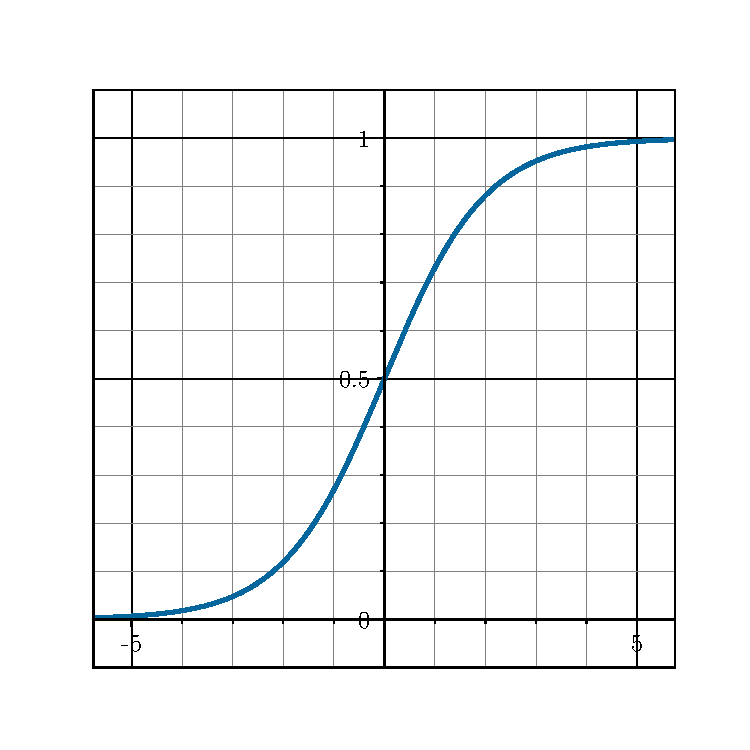
\includegraphics[width=0.98\textwidth]{figures/main/ch2-background/sigmoid.pdf}
    \caption{Sigmoid Activation}
  \end{subfigure}
  \hfill
  \begin{subfigure}[b]{0.32\textwidth}
    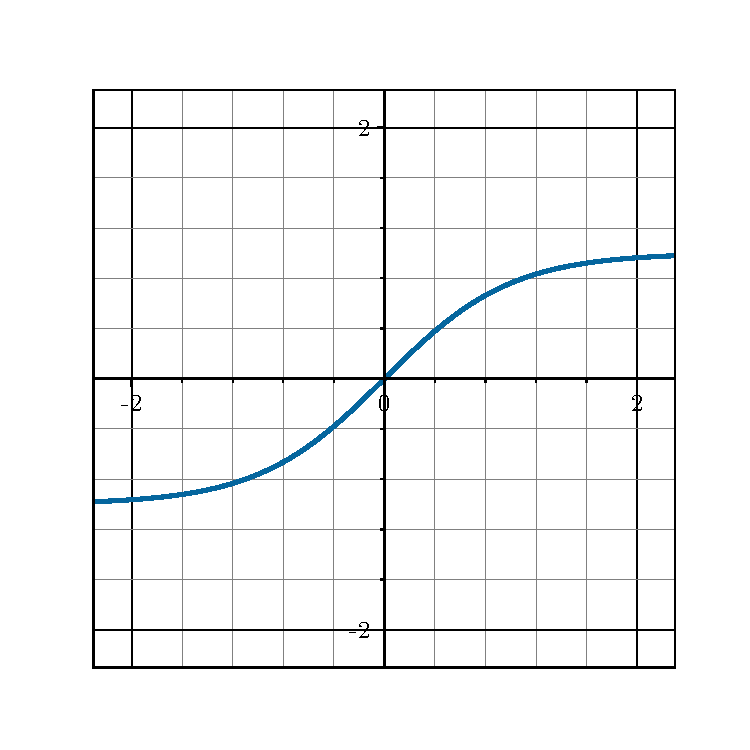
\includegraphics[width=0.98\textwidth]{figures/main/ch2-background/tanh.pdf}
    \caption{Tanh Activation}
  \end{subfigure}
  \hfill
  \begin{subfigure}[b]{0.32\textwidth}
    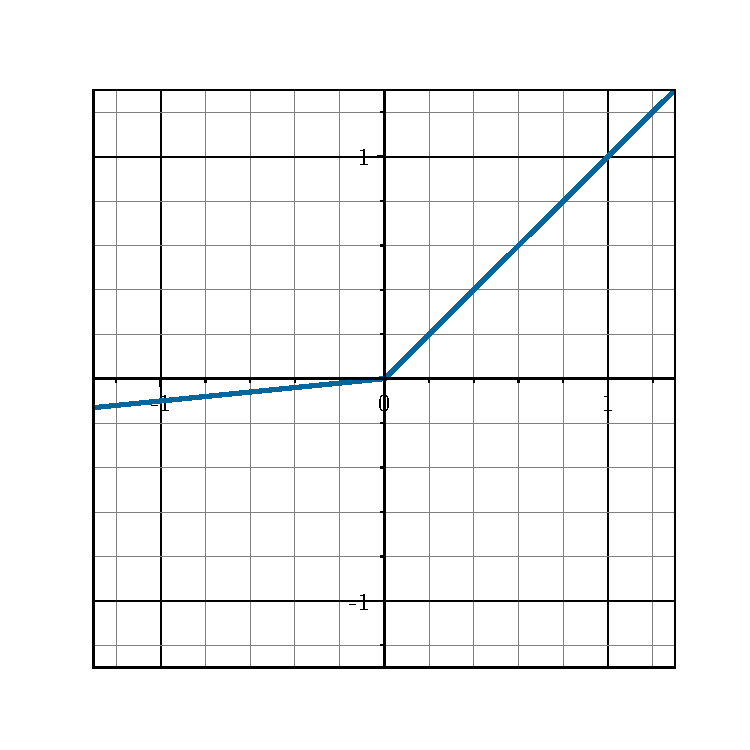
\includegraphics[width=0.98\textwidth]{figures/main/ch2-background/relu.pdf}
    \caption{Leaky ReLU Activation}
  \end{subfigure}
  \caption{Graphical representation of 3 common activation functions}
  \label{figure:ch2-activation_functions}
\end{figure}


Choosing the right activation function has been an active area of research. 
Hereafter, we present 3 common activation functions used by practitioners.
\begin{itemize}
  \item \textbf{Sigmoid activation} \cite{han1995influence}
    \begin{equation*}
      \act(x) = \frac{1}{1+e^{-x}} 
    \end{equation*}
    The sigmoid activation function is one of the first continuous non-linear function to be used in the context of neural network. It takes a real value as input and outputs another value between 0 and 1.
  \item \textbf{Hyperbolic Tangent activation} \cite{karlik2011performance}
    \begin{equation*}
      \act(x) = \frac{e^x - e^{-x}}{e^x + e^{-x}}
    \end{equation*}
    The hyperbolic tangent activation function is similar to the sigmoid activation function but instead of returning between 0 and 1, the function returns between -1 and 1.     
  \item \textbf{Leaky Rectified Linear activation (Leaky-ReLU)} \cite{maas2013rectifier}
    \begin{equation*}
      \act(x) = \max(\alpha, x)
    \end{equation*}
    More recently, the ReLU~\cite{nair2010rectified} ($\alpha = 0$) and leaky-ReLU~\cite{maas2013rectifier} ($\alpha > 0$) activation function was proposed.
    The parameter $\alpha$ characterize the slope on $\Rbb_-$.
    These function have the advantages to avoids the vanishing gradient problem and are less less computationally expensive than tanh and sigmoid because it involves simpler mathematical operations.
\end{itemize}

\noindent
The \Cref{figure:ch2-activation_functions} present the graphical representation of the 3 activation functions presented above.
In this thesis, we will exclusively use the Leaky-ReLU function with different $\alpha$ when we train deep neural networks.
Therefore, we simplify the notation $\nn^\act_\weights$ with $\nn_\weights$.


The architecture of a neural network is governed by mainly two factors: the dimensions of the hidden layers and the depth of the network.
Different types of scaling have been studied.
Neural networks with large width have been studied both theoretically and experimentally.
\citet{cybenko1989approximation,hornik1989multilayer} have shown that neural networks with a single hidden layer and sigmoid activation can approximate any function if the hidden layer is allowed to be arbitrary large. 
However, wide and shallow networks tend to be difficult to train due to having difficulties in capturing higher-level features. 
Indeed, it has been empirically observed that deep neural networks tend to achieve greater performance that large and shallow neural networks.
More recently, the \emph{universal approximation result} have been extended to bounded width neural network with arbitrary depth~\cite{lu2017expressive,hanin2017universal}.
More formally, we have the following result for neural networks with $\relu$ activations:
\begin{maintheorem}[Universal Approximation Theorem for Neural Network \citet{hanin2017universal}]
  For any continuous function $f:[0,1]^{n} \rightarrow \mathbb{R}_+$ of bounded supremum norm, for any $\epsilon>0$, there exists a neural network $\nn_\weights$ parametried by $\weights$ with an input layer of width $n$, an output layer of width $1$, hidden layers of width $n+3$ and ReLU activations such that 
  \begin{equation}
    \forall x \in [0,1]^n, \quad \left| f(\xvec) - \nn_\weights(\xvec) \right| < \epsilon \enspace.
  \end{equation}
  \vspace{-2em}
\end{maintheorem}


% From $\mathcal{N}$, we can easily build a deep ReLU network $\mathcal{N'}$ of width exactly $n+3$, such that $\forall x \in [0,1]^{n+3}$, $\left|f(\xvec_{1} \ldots \xvec_{n}) - \left(\mathcal{N}'\left(\xvec\right)\right)_{1}\right| < \epsilon$. Thanks to \Cref{lemma:dcnn_approx_neural_network}, this last network can be approximated arbitrarily well by a DCNN of width $n+3$.
%
% \begin{theorem}
%   Let $\mathcal{X} \subset \Rbb^{w_{(1)}}$.
%   For any continuous function $f: \mathcal{X} \rightarrow \Rbb^{w^{(\depth)}}$, then there exists a  
%
%   Let $\mathcal{X} \subset \Rbb^{w_{(1)}}$ and let $f: \Rbb^{w^{(1)}} \rightarrow \Rbb^{w^{(\depth)}}$ be a continuous function.
%   Then, there exists a neural networks parameterized by $\weights$ with an input dimension $w^{(1)}$, an arbitrary depth $\depth$, and $\relu$ activation such that:
%   \begin{equation}
%     \norm{f(\xvec) - \nn(\xvec)} \leq \epsilon
%   \end{equation}
%   \label{theorem:ch2-universal_approximation_theorem}
% \end{theorem}
%


% \citet{cybenko1989approximation} have shown that shallow neural networks with sigmoid activation can \emph{theoretically} approximate any decision boundary.
%
% The arbitrary depth case was also studied by number of authors, such as Zhou Lu et al in 2017,[11] 
% \cite{lu2017expressive}
%
% Boris Hanin and Mark Sellke in 2018,[12] 
% \cite{hanin2017universal}





%%%%%%%%%%%%%%%%%%%%%%%%%%%%%%%%%%%%%%%%%%%%%%%%%%%%%%%%%%%%%%%%%%%%%%%%%%%%%%%
\section{Adversarial Attacks \& Robustness of Neural Networks}
\label{section:ch2-preliminaries_on_adversarial_attacks}
%%%%%%%%%%%%%%%%%%%%%%%%%%%%%%%%%%%%%%%%%%%%%%%%%%%%%%%%%%%%%%%%%%%%%%%%%%%%%%%

As seen in the introduction (\Cref{chapter:ch1-introduction}), deep neural networks achieve state-of-the-art performances in a variety of domains such as natural language processing~\cite{radford2018Language}, image recognition~\cite{he2016deep} and speech recognition~\cite{hinton2012deep}.
However, it has been shown that such neural networks are vulnerable to \emph{adversarial examples}, \ie, imperceptible variations of the natural examples, crafted to deliberately mislead the models~\cite{globerson2006nightmare,biggio2013evasion,szegedy2013intriguing}.
Because it is difficult to characterize the space of visually imperceptible variations of a natural image, existing adversarial attacks use $\ell_p$ norms as surrogates measure.
We can formally define an adversarial example as follows:
\begin{definition}[Adversarial Pertubation]
  Given a dataset $\mathcal{S} = \mathcal{X} \times \mathcal{Y}$, a pair $(\xvec, y) \sim \mathcal{S}$ and a trained neural network $\nn_\weights$ on $\mathcal{S}$ such that $\argmax_{i \in [k-1]_0} \{ \nn_\weights(\xvec)_i \} = y$, let $\adv \in \mathcal{X}$ be an adversarial perturbation such that:
  \begin{align}
    &\argmax_{i \in [k-1]_0} \{ \nn_\weights (\xvec + \adv)_i \} \neq y \\
    \st\ &\norm{\adv}_p \leq \epsilon \notag
  \end{align}
  where $\epsilon$ is a small value defined by the attacker. 
\end{definition}

%%%%%%%%%%%%%%%%%%%%%%%%%%%%%%%%%%%%%%%%%%%%%%%%%%%%%%%%%%%%%%%%%%%%%%%%%%%%%%%
\subsection{Implementing Adversarial Attacks}
\label{subsection:ch2-adversarial_attacks}
%%%%%%%%%%%%%%%%%%%%%%%%%%%%%%%%%%%%%%%%%%%%%%%%%%%%%%%%%%%%%%%%%%%%%%%%%%%%%%%

Since the discovery of adversarial perturbations, a variety of procedures, \aka \emph{adversarial attack}, have been developed to generate adversarial examples, for example FGSM \cite{goodfellow2014explaining}, PGD \cite{madry2018towards} and C\&W \cite{carlini2017towards}, to mention the most popular ones.
To find the best perturbation $\adv$, existing attacks can adopt one of the two following strategies:
% \begin{itemize}
%   \item \textbf{Loss maximization}: maximizing the loss $L(\nn_\weights(\xvec + \adv), y)$ under some constraint on $\norm{\adv}_p$ with $p \in \{0, \dots, \infty\}$.;
%   \item \textbf{Perturbation minimization}: minimizing $\norm{\adv}_p$ under some constraint on the loss $L(\nn_\weights(\xvec + \adv), y)$.
% \end{itemize}

\paragraph{Loss maximization.}
In this scenario, the procedure maximizes the loss objective function $L(\nn_\weights(\xvec + \adv), y)$, under the constraint that the $\lp$ norm of the perturbation remains bounded by some value $\epsilon$, as follows:
\begin{equation}
  \argmax_{\adv:\norm{\adv}_p \leq \epsilon} L(\nn_\weights(\xvec + \adv), y) \enspace.
  \label{equation:ch2-lossmax}
\end{equation}
The typical value of $\epsilon$ depends on the norm $\norm{\ \cdot\ }_p$ considered in the problem setting.
% In order to compare $\linf$ and $\ltwo$ attacks of similar strength, we choose values of $\epsilon_\infty$ and $\epsilon_2$ (for $\linf$ and $\ltwo$ norms respectively) which result in $\linf$ and $\ltwo$ balls of equivalent volumes.
% For the particular case of CIFAR-10, this would lead us to choose $\epsilon_\infty = 0.03$ and $\epsilon_2 = 0.8$ which correspond to the maximum values chosen empirically to avoid the generation of visually detectable perturbations. 
The current state-of-the-art method to solve \Cref{equation:ch2-lossmax} is based on a projected gradient descent (PGD)~\cite{madry2018towards} of radius~$\epsilon$.
Given a budget $\epsilon$, it recursively computes
\begin{equation}
  \xvec^{(t+1)} = \prod_{\mathcal{B}_p(\xvec,\epsilon)}\left(\xvec^{(t)}
    + \alpha \argmax_{\adv: \norm{\adv}_p \leq 1} \nabla_\xvec L\left( \nn_\weights \left(\xvec^{(t)} + \adv \right), y \right)
\right)
  \label{equation:ch2-projectionPGD}
\end{equation}
where $\mathcal{B}_p(\xvec,\epsilon) = \{ \xvec + \adv:\norm{\adv}_p \leq \epsilon\}$, $\alpha$ is a gradient step size, and $\prod_S$ is the projection operator on $S$.
The PGD attack is currently used in the literature with $p=2$ and $p=\infty$.
The attack with the norm $p=\infty$ is state-of-the-art for the loss maximization problem. 

\paragraph{Perturbation minimization.}
This type of procedure search for the perturbation that has the minimal $\lp$ norm, under the constraint that $L(\nn_\weights(\xvec + \adv), y)$ is bigger than a given bound $c$:
\begin{align}
  &\argmin_{\adv} \norm{\adv}_p \label{equation:ch2-normmin} \\
  \st\ &L(\nn_\weights(\xvec + \adv), y) \geq c \notag
\end{align}
The value of $c$ is typically chosen depending on the loss function $L$. For example, if $L$ is the $0-1$ loss, any $c > 0$ is acceptable.
\Cref{equation:ch2-normmin} has been tackled by~\citet{carlini2017towards}, leading to the following method, denoted C\&W attack in the rest of the chapter. It aims at solving the following Lagrangian relaxation of \Cref{equation:ch2-normmin}:
\begin{equation}
  \argmin_{\adv} \norm{\adv}_p + \lambda g(\xvec+\adv)
\end{equation}
where $g(\xvec + \adv)<0$ if and only if $L(\nn_\weights(\xvec + \adv),y) \geq c$. 
The authors use a change of variable $\adv = \tanh(\wvec) - \xvec$ to ensure that $\xvec + \adv \in \mathcal{X}$, a binary search to optimize the constant $c$, and Adam or SGD to compute an approximated solution.
The C\&W attack is currently used in the literature with $p \in \{1, 2, \infty \}$ and is state-of-the-art with $p=2$ for the perturbation minimization problem
% This attack with the norm $p=2$ is state-of-the-art for the perturbation minimization problem. 
% The C\&W attack is well defined both for $p=2$, and $p=\infty$, but there is a clear empirical gap of efficiency in favor of the $\ltwo$ attack.


% For example, \citet{goodfellow2014explaining} use the $\linf$ norm to measure the distance between the original image and the adversarial image whereas \citet{carlini2017towards} use the $\ltwo$ norm.
% When the input dimension is low, the choice of the norm is of little importance because the $\linf$ and $\ltwo$ balls overlap by a large margin, and the adversarial examples lie in the same space.
% For typical image datasets with large dimensionality, the two balls are mostly disjoint.
% As a consequence, the $\linf$ and the $\ltwo$ adversarial examples lie in different areas of the space, and it explains why $\linf$ defense mechanisms perform poorly against $\ltwo$ attacks and vice versa. 



%%%%%%%%%%%%%%%%%%%%%%%%%%%%%%%%%%%%%%%%%%%%%%%%%%%%%%%%%%%%%%%%%%%%%%%%%%%%%%%
\subsection{Defending against Adversarial Attacks}
\label{subsection:ch2-defending_against_adversarial_attacks}
%%%%%%%%%%%%%%%%%%%%%%%%%%%%%%%%%%%%%%%%%%%%%%%%%%%%%%%%%%%%%%%%%%%%%%%%%%%%%%%

Given the important security risks that adversarial attacks pose, it is important to design defenses to protect neural networks against these kinds of attacks.
Adversarial Training was introduced by~\citet{goodfellow2014explaining} and later improved by~\citet{madry2018towards} as a first defense mechanism to train robust neural networks.
It consists in augmenting training batches with adversarial examples generated during the training procedure.
The structural risk minimization paradigm is thus replaced by the following $\min$ $\max$ problem, where the classifier tries to minimize the expected loss under maximum perturbation of its input:
\begin{equation}
  \argmin_\weights \argmax_{\adv: \norm{\adv} \leq \epsilon} \frac{1}{|\mathcal{S}|} \sum_{(\xvec, y) \in \mathcal{S}} L\left( \nn_\weights \left(\xvec + \adv \right), y \right) + \lambda \sum_{(\Wmat, \bvec) \in \weights} \left( \norm{\Wmat}_\mathrm{F} + \norm{\bvec}_\mathrm{2} \right)
\end{equation}
% In the case where $p = \infty$, this technique offers good robustness against $\linf$ attacks \cite{athalye2018obfuscated}.
Although adversarial training lacks formal guarantees, it is one of the few techniques that prove to be empirically very effective.


% Despite some recent work providing great insights \cite{sinha2017certifying,zhang2019theoretically}, there is no worst case lower bound yet on the accuracy under attack of this method.




% \%\%\%
%
% \cite{goodfellow2014explaining} have proposed \textbf{Adversarial Training} which follows \textbf{ERM} training over adversarially-perturbed samples
%
%
% \%\%\%

% Another important technique to defend against adversarial examples is to use \emph{noise injection} techniques.  
% In contrast with adversarial Training, noise injection mechanisms are usually deployed after training.


% In a nutshell, it works as follows.
% At inference time, given a unlabeled sample $x$, the network outputs
% \begin{equation}
%   \tilde{f}_\theta(\xvec) \triangleq f_\theta(\xvec + \eta) \ \ \ (\text{instead of  } f_\theta(\xvec)) 
% \end{equation}
% where $\eta$ is a random variable on $\mathbb{R}^d$.
% Even though, Noise Injection is often less efficient than Adversarial Training in practice (see \eg, \Cref{table:764774}), it benefits from strong theoretical background.
% In particular, recent works \cite{lecuyer2018certified,li2019certified}, followed by~\citet{cohen2019certified,pinot2019theoretical} demonstrated that noise injection from a Gaussian distribution can give provable defense against $\ltwo$ adversarial attacks.
% In this work, besides the classical Gaussian noises already investigated in previous works, we evaluate the efficiency of Uniform distributions to defend against $\ltwo$ adversarial examples. 




%%%%%%%%%%%%%%%%%%%%%%%%%%%%%%%%%%%%%%%%%%%%%%%%%%%%%%%%%%%%%%%%%%%%%%%%%%%%%%%
\section{A Primer on Toeplitz and Circulant Matrices}
\label{section:ch2-a_primer_on_toeplitz_and_circulant_matrices}
%%%%%%%%%%%%%%%%%%%%%%%%%%%%%%%%%%%%%%%%%%%%%%%%%%%%%%%%%%%%%%%%%%%%%%%%%%%%%%%

In this thesis, we make contributions at the intersection between neural networks and structured matrices.
We build neural networks with structured matrices and develop new algorithms for training neural networks based on certain properties of structured matrices. 
Hereafter, we present some preliminaries on structured matrices that we will use later. 

%%%%%%%%%%%%%%%%%%%%%%%%%%%%%%%%%%%%%%%%%%%%%%%%%%%%%%%%%%%%%%%%%%%%%%%%%%%%%%%
\subsection{Toeplitz Matrices}
\label{subsection:ch2-toeplitz_matrices}
%%%%%%%%%%%%%%%%%%%%%%%%%%%%%%%%%%%%%%%%%%%%%%%%%%%%%%%%%%%%%%%%%%%%%%%%%%%%%%%

A Toeplitz matrix, named after Otto Toeplitz, is a matrix in which each descending diagonal from left to right is constant.
Let $P = \{-n+1, \dots, n-1\}$, an $n\times n$ Toeplitz matrix $\Amat$ is fully determined by a two-sided sequence of scalars $\{a_h\}_{h \in P}$ as follows:
\begin{equation}
  \Amat =
  \leftmatrix
    a_0 & a_{1} & a_{2} & \cdots & \cdots & a_{n-1} \\
    a_{-1} & a_0 & a_{1} & \ddots & & \vdots \\
    a_{-2} & a_{-1} & \ddots & \ddots & \ddots & \vdots \\
    \vdots & \ddots & \ddots & \ddots & a_{1} & a_{2} \\
    \vdots & & \ddots & a_{-1} & a_{0} & a_{1} \\
    a_{-n+1} & \cdots & \cdots & a_{-2} & a_{-1} & a_0
  \rightmatrix
\end{equation}
\noindent
Because the Toeplitz matrix $\Amat$ is fully determined by the sequence $\{a_h\}_{h \in P}$, it can be compactly represented in memory using only $2n-1$ values instead of $n^2$.
Toeplitz matrices can also be characterized by noting that the $(k,j)$ entry of $\Amat$, $\leftmat \Amat \rightmat_{j,k}$ is given by
\begin{equation}
  \leftmat \Amat \rightmat_{j,k} = a_{k-j} \enspace.
\end{equation}

A standard tool for manipulating Toeplitz matrices is the use of Fourier analysis.
Let $\{a_h\}_{h \in P}$ be the sequence of coefficients of the Toeplitz matrix $\Amat \in \mathbb{R}^{n\times n}$.
The complex-valued function 
\begin{equation}
  f(\omega) = \sum_{h \in P} a_h e^{\ci h \omega}
\end{equation}
is the \emph{inverse Fourier transforms} of the sequences $\{a_h\}_{h \in P}$ with $\omega \in \mathbb{R}$.
From this function, one can recover the sequence $\{a_h\}_{h \in P}$ using the standard Fourier transform:
\begin{equation}
  a_h = \frac{1}{2\pi} \int_0^{2\pi} e^{-\ci h \omega} f(\omega) d\omega \enspace. 
\end{equation}

From there, similarly to the work done by~\citet{gray2006toeplitz}, we can define an operator $\Tmat$ mapping integrable functions to matrices:
\begin{equation}
  \Tmat_n(g) \triangleq \leftmat\frac{1}{2\pi}\int_{0}^{2\pi}e^{-\ci(i-j)\omega}g(\omega)\,d\omega\rightmat_{i,j\in\{0,\ldots,n-1\}} \enspace.
  \label{equation:ch2-toeplitz_operator}
\end{equation}
\noindent
In the following of this thesis, when it is clear from context, we will write $\Tmat(g)$ instead of $\Tmat_n(g)$.
We can show that if $f$ is the inverse Fourier transform of $\{a_h\}_{h \in P}$, then $\Tmat_n(f)$ is equal to $\Amat$.
\begingroup
\allowdisplaybreaks
  \begin{align}
      \leftmat \Tmat_n(f) \rightmat_{i, j} &= \frac{1}{2\pi} \int_0^{2\pi} e^{-\ci (i-j)\omega} f(\omega) \,d\omega  \\
      &= \frac{1}{2\pi} \int_0^{2\pi} e^{-\ci (i-j) \omega} \sum_{h \in N} a_h e^{\ci h \omega} \,d\omega  \\
      &= \frac{1}{2\pi} \int_0^{2\pi} \sum_{h \in N} a_h e^{\ci (j - i + h) \omega} \,d\omega  \\
      &= \sum_{h \in N} a_h \frac{1}{2\pi} \int_0^{2\pi} e^{\ci (j - i + h) \omega} \,d\omega 
      = a_{j-i} .
  \end{align}
\endgroup
Because:
\begin{equation}
  \frac{1}{2\pi} \int_0^{2\pi} e^{\ci k \omega} \,d\omega = 
  \begin{cases}
    1 \quad \text{if}\ k = 0, \\
    0 \quad \text{if}\ k\ \text{is a non-zero integer number.}
  \end{cases}
\end{equation}

% Also, if $F$ is the inverse Fourier transform of $\{\Bmat_h\}_{h \in P}$ as defined above, then the integral in \Cref{equation:expression_toeplitz_matrix} is matrix-valued, and thus $\Tmat(F) \in \mathbb{R}^{mn \times mn}$ is the block matrix $\Bmat$.

% The trigonometric polynomial that \emph{generates} the Toeplitz matrix $\Amat$ can be defined as follows:
% \begin{equation}
%   f_{\Amat}(\omega) \triangleq \sum_{h \in N} a_h e^{\ci h \omega}
% \end{equation}
% The function $f_{\Amat}$ is said to be the \emph{generating function} of $\Amat$.
% To recover the Toeplitz matrix from its generating function, we have the following operator:
% \begin{equation}
%   \leftmat \Tmat(f) \rightmat_{i, j} \triangleq \frac{1}{2\pi} \int_0^{2\pi} e^{-\ci (i - j)\omega} f(\omega) \,d\omega .
%   \label{equation:ch2-toeplitz_operator}
% \end{equation}


%%%%%%%%%%%%%%%%%%%%%%%%%%%%%%%%%%%%%%%%%%%%%%%%%%%%%%%%%%%%%%%%%%%%%%%%%%%%%%%
\subsection{Circulant Matrices}
\label{subsection:ch2-circulant_matrices}
%%%%%%%%%%%%%%%%%%%%%%%%%%%%%%%%%%%%%%%%%%%%%%%%%%%%%%%%%%%%%%%%%%%%%%%%%%%%%%%

Circulant matrices are a special case of Toeplitz matrices.
In addition to having constant diagonals, each row of a circulant matrix is a cyclic right shift of the previous one.
% Circulant matrices have been used to efficiently solve linear systems~\cite{golub1996matrix} and years later were used to perform dimensionality reduction~\cite{hinrichs2011johnson,vybiral2011variant}, binary embedding~\cite{yu2014circulant} and kernel approximation~\cite{yu2015compact} in the context of pattern recognition and machine learning.
An $n \times n$ circulant matrix $\Cmat$ is fully determined by a sequence of scalars $\{c_h\}_{h \in [n-1]_0}$ as follows:

\begin{equation}
  \Cmat =
  \leftmatrix
    c_0 & c_{n-1} & c_{n-2} & \cdots & \cdots & c_{1} \\
    c_{1} & c_0 & c_{n-1} & \ddots & & \vdots \\
    c_{2} & c_{1} & \ddots & \ddots & \ddots & \vdots \\
    \vdots & \ddots & \ddots & \ddots & c_{n-1} & c_{n-2} \\
    \vdots & & \ddots & c_{1} & c_{0} & c_{n-1} \\
    c_{n-1} & \cdots & \cdots & c_{2} & c_{1} & c_0
  \rightmatrix
\end{equation}

Because the circulant matrix $\Cmat$ is fully determined by the sequence $\{c_h\}_{h \in [n-1]_0}$, it can be compactly represented in memory using only $n$ values instead of $n^2$.
Circulant matrices can also be characterized by noting that the $(k,j)$ entry of $\Cmat$, $\leftmat \Cmat \rightmat_{j,k}$ is given by
\begin{equation}
  \leftmat \Cmat \rightmat_{j,k} = c_{\left(k-j\right) \mod n} \enspace.
\end{equation}
% We can also denote the sequence $\{c_h\}$ as a vector $\cvec$ such that $\forall i, \cvec_i = c_i$. The circulant matrices can then be expressed with $\Cmat = \circulant(\cvec)$.
Circulant matrices exhibit several interesting properties which are based on the fact that they can be diagonalized by the Discrete Fourier Transform (DFT)~\cite{davis1979circulant}.
First, we define the Fourier Matrix and then, we present an important theorem regarding eigenvalues and eigenvectors of circulant matrices circulant matrices.

\begin{definition}[Fourier Matrix]
  The Fourier matrix of order $n$ is defined as follows:
  \begin{equation}
    \Umat_n = 
    \leftmatrix
      1      & 1           & 1              & \cdots & 1           \\
      1      & z_n       & z_d^2        & \cdots & z_d^{d-1} \\
      1      & z_n^2     & z_d^4        & \cdots & z_d^{2(d-1)} \\
      \vdots & \vdots      & \vdots         &        & \vdots      \\
      1      & z_n^{n-1} & z_d^{2(n-1)} & \cdots & z_d^{(d-1)(d-1)}
    \rightmatrix
  \end{equation}
  where $z_n = e^{-\frac{2\pi\ci}{n}}$ is an $n^{\text{th}}$ root of unity.
  \label{definition:ch2-fourier_matrix}
\end{definition}
\noindent
The matrix-vector product between the Fourier matrix above and a vector is equivalent to apply the Discrete Fourier Transform on the vector.
This matrix-vector product can be efficiently computed with the \emph{Fast Fourier transform} (FFT) algorithm~\cite{cooley1965algorithm}.
The complexity is reduced from from $\mathcal{O}(n^2)$ to $\mathcal{O}(n \log n)$.

\begin{theorem}[Theorem 3.1 of \citet{gray2006toeplitz}]
  Every $n \times n$ circulant matrix $\Cmat$, has eigenvectors  
  \begin{equation}
    \yvec^{(k)} = \frac{1}{\sqrt{n}} \leftmatrix 1, e^{-\frac{2 \pi \ci k}{n}}, \dots, e^{-\frac{2 \pi \ci k(n-1)}{n}} \rightmatrix^\top
  \end{equation}
  and corresponding eigenvalues
  \begin{equation}
    \psi_k = \sum_{j=0}^{n-1} c_j e^{-\frac{2 \pi \ci}{n} jk}
  \end{equation}
  The circulant matrix $\Cmat$ can be expressed in the form 
  \begin{equation}
    \Cmat = \frac{1}{n} \Umat_n^* \diag(\Umat_n \cvec) \Umat_n
    \label{equation:ch2-diagonalization_circulant_matrix}
  \end{equation}
  where $\cvec$ is vector based of the scalars $\{c_h\}_{h \in [n-1]_0}$.
  In particular all circulant matrices share the same eigenvectors, the same matrix $\Umat_n$ works for all $n \times n$ circulant matrices.
  Also, if $\Cmat$ and $\Bmat$ are circulant matrices then $\Cmat$ and $\Bmat$ commute and $\Cmat + \Bmat$ is also a circulant matrix.
  \label{theorem:ch2-diagonalization_circulant_matrix}
\end{theorem}
\noindent
Based on \Cref{theorem:ch2-diagonalization_circulant_matrix} and of the \emph{Fast Fourier transform} (FFT) algorithm the matrix-vector product between a circulant matrix $\Cmat$ and a vector $\xvec$ can be reduced from $\mathcal{O}(n^2)$ to $\mathcal{O}(n \log n)$. 
If we denote the Fast Fourier transform algorithm by \textbf{FFT} and the inverse by \textbf{IFFT}, the pseudocode for the matrix-product between a circulant matrix and a vector is as follows:
\begin{algorithm}[h]
  \begin{algorithmic}[1]
    \Procedure{input}{$\cvec, \xvec$} \Comment{first column of the circulant matrix $\Cmat$, vector $\xvec$}
      \State $\tilde{\xvec} \gets \textbf{FFT}(\xvec)$
      \State $\tilde{\cvec} \gets \textbf{FFT}(\cvec)$
      \State $\yvec \gets \textbf{IFFT}(\tilde{\xvec} * \tilde{\cvec})$ \Comment{element-wise vector-vector product}
      \State \textbf{return} $\yvec$ \Comment{return the result of the product $\Cmat \xvec$}
    \EndProcedure
  \end{algorithmic}
  \caption{Matrix-vector product with a circulant matrix}
  \label{algorithm:ch2-matrix_vector_product_circulant_matrix}
\end{algorithm}

An important object based on circulant matrices are called \emph{$f$-circulant matrices} and are defined as follows:
\begin{definition}[$f$-circulant matrix]
  Given a vector $\xvec$, the $f$-circulant matrix, $\Zmat_f(\xvec)$, is defined as follows:
  \begin{equation}
    \Zmat_f(\xvec) \triangleq
    \leftmatrix
      \xvec_0 & $f$ \xvec_{n-1} & $f$ \xvec_{n-2} & \cdots & \cdots & $f$ \xvec_{1} \\
      \xvec_{1} & \xvec_0 & $f$ \xvec_{n-1} & \ddots & & \vdots \\
      \xvec_{2} & \xvec_{1} & \ddots & \ddots & \ddots & \vdots \\ 
      \vdots & \ddots & \ddots & \ddots & $f$ \xvec_{n-1} & $f$ \xvec_{n-2} \\
      \vdots & & \ddots & \xvec_{1} & \xvec_{0} & $f$ \xvec_{n-1} \\
      \xvec_{n-1} & \cdots & \cdots & \xvec_{2} & \xvec_{1} & \xvec_0
    \rightmatrix
  \end{equation}
  \label{definition:ch2-f_circulant_matrix}
\end{definition}
\noindent
A $f$-unit-circulant, denoted $\Zmat_f$, is a $f$-circulant matrix defined by the vector $\left(0, 1, \dots, 0 \right)$:
\begin{equation}
  \Zmat_f = \circulant \left(e^{(1)} \right) + (f - 1) \evec^{(0)} \evec^{(n-1)\top} = 
    \leftmatrix
      0      & 0      & 0      & \cdots & \cdots & f      \\
      1      & 0      & 0      & \ddots &        & \vdots \\
      0      & 1      & \ddots & \ddots & \ddots & \vdots \\ 
      \vdots & \ddots & \ddots & \ddots & 0      & 0      \\
      \vdots &        & \ddots & 1      & 0      & 0      \\
      0      & \cdots & \cdots & 0      & 1      & 0
    \rightmatrix
\end{equation}

\noindent
As stated by~\citet{sindhwani2015structured}, the $f$-unit-circulant matrix performs a downward shift-and-scale transformation on a vector.
More precisely, the matrix-vector product $\Zmat_f \xvec$ makes a circular shifts on the elements and scale the last element of the vector resulting in $\Zmat_f \xvec = \leftmat f \xvec_{n-1}, \xvec_0, \dots, \xvec_{n-2} \rightmat^\top$. 
$f$-unit-circulant matrix are one of the building block of \emph{Low displacement rank operator} presented in \Cref{subsection:ch3-building_compact_neural_networks_with_structured_matrices}.


% The f-unit-circulant matrix is associated with a basic downward shift-and-scale transformation, i.e.,
% the matrix-vector product Zfv shifts the elements of the column vector v “downwards”, and scales
% and brings the last element vn to the “top”, resulting in [fvn, v1, . . . vn−1] T .
% It has several basic
% algebraic properties (see Proposition 1.1 [1]) that are crucial for the results stated in this section



% the complexity of the matrix-vector product between a circulant matrix $\Cmat$ and a vector $\xvec$ can be reduced from $\mathcal{O}(n^2)$ to $\mathcal{O}(n \log n)$ with the \emph{Fast Fourier transform} (FFT) algorithm~\cite{cooley1965algorithm}.

% More precisely, the eigenvalues $\psi_k$ of the matrix $\Cmat$ correspond to the discrete Fourier transform of the vector characteristic $\cvec$:
% and the eigenvectors $\yvec^{(k)}$ can be expressed as follows:
% \begin{equation}
%   \yvec^{(k)} = \frac{1}{\sqrt{n}} \leftmatrix 1, e^{-\frac{2 \pi \ci k}{n}}, \dots, e^{-\frac{2 \pi \ci k(n-1)}{n}} \rightmatrix^\top
% \end{equation}
% In matrix form, we can diagonalize the matrix $\Cmat$ as follows:
% \begin{equation}
%   \Cmat = \frac{1}{n} \Umat_n^* \diag(\Umat_n \cvec) \Umat_n
% \end{equation}
% where $\Umat_n = \leftmatrix e^{-\frac{2 \pi \ci jk}{n}} \rightmatrix_{j,k = 0}^{n-1}$ is the DFT matrix and $\cvec$ is vector based of the scalars $\{c_h\}_{h \in \{0, \dots, n-1\}}$.

% The following Theorem summarize the propreties for circulant matrices derived above.



\comment{


%%%%%%%%%%%%%%%%%%%%%%%%%%%%%%%%%%%%%%%%%%%%%%%%%%%%%%%%%%%%%%%%%%%%%%%%%%%%%%%
\subsection{Relationship between Toeplitz and circulant matrices}
\label{subsection:ch2-relationship_between_toeplitz_and_circulant_matrices}
%%%%%%%%%%%%%%%%%%%%%%%%%%%%%%%%%%%%%%%%%%%%%%%%%%%%%%%%%%%%%%%%%%%%%%%%%%%%%%%

\todotext{completer ici}


This assumption is justified by the work of \citet{gray2006toeplitz,gutierrez2012block} which states that a sequence of block Toeplitz matrices is asymptotically equivalent to a sequence of sequence of block circulant matrices.

The concept of asymptotically equivalent sequences can be illustrated by the following. 
Consider the infinite sequence $\{a_k\}$ and define the corresponding $n \times n$ Toeplitz operator $\Tmat(n) = \leftmat a_{k-j} \rightmat_{k,j = 0}^{n-1}$.
We call \emph{banded}-Toeplitz matrix, a Toeplitz matrix for which it exists an $m$ such that $a_k = 0$, for $|k| > m$.
A $n \times n$ banded-Toeplitz matrix can be represented as follows:
\begin{equation}
  \Tmat(n)  =
  \leftmatrix
    a_0    & a_1    & \cdots   & a_m    &        &        &        &        &        &        \\
    a_{-1} & a_0    & a_1      &        & \ddots &        &        &        &        &        \\
    \vdots & a_{-1} & \ddots   & \ddots &        & \ddots &        & 0      &        &        \\
    a_{-m} &        & \ddots   & \ddots & \ddots &        & a_m    &        &        &        \\ 
           & \ddots &          & \ddots & a_0    & a_1    &        & \ddots &        &        \\
	   &        & \ddots   &        & a_{-1} & \ddots & \ddots &        & \ddots &        \\
	   &        &          & a_{-m} &        & \ddots & \ddots & \ddots &        & a_m    \\
    	   &        & 0        &        & \ddots &        & \ddots & \ddots & a_1    & \vdots \\
           &        &          &        &        & \ddots &        & a_{-1}  & a_0    & a_1   \\  
           &        &          &        &        &        & a_{-m} & \cdots & a_{-1} & a_0    \\ 
  \rightmatrix
\end{equation}
\citet{gray2006toeplitz} has noted that the only difference between a $n \times n$ banded-Toeplitz matrix and a circulant matrix based on the same sequence is the values on the bottom-left and top-right corner of the matrix.
The circulant matrix based on the same sequence $\{a_k\}$ can be represented as follows:
\begin{equation}
  \Cmat(n)  =
  \leftmatrix
    a_0    & a_1    & \cdots   & a_m    &        &        &        & a_{-m} & \cdots & a_{-1} \\
    a_{-1} & a_0    & a_1      &        & \ddots &        &        &        & \ddots & \vdots \\
    \vdots & a_{-1} & \ddots   & \ddots &        & \ddots &        & 0      &        & a_{-m} \\
    a_{-m} &        & \ddots   & \ddots & \ddots &        & a_m    &        &        &        \\ 
           & \ddots &          & \ddots & a_0    & a_1    &        & \ddots &        &        \\
	   &        & \ddots   &        & a_{-1} & \ddots & \ddots &        & \ddots &        \\
	   &        &          & a_{-m} &        & \ddots & \ddots & \ddots &        & a_m    \\
    a_m	   &        & 0        &        & \ddots &        & \ddots & \ddots & a_1    & \vdots \\
    \vdots & \ddots &          &        &        & \ddots &        & a_{-1} & a_0    & a_1    \\  
    a_1    & \cdots & a_m      &        &        &        & a_{-m} & \cdots & a_{-1} & a_0    \\ 
  \rightmatrix
\end{equation}
\noindent
Thus, the greater the difference between $n$ and $m$, the `closer' the banded-Toeplitz matrix will be to the circulant one. 
This concept of closeness between Toeplitz and a circulant matrix have been extensively studied and extended to block Toeplitz and block circulant matrices~\cite{Toeplitz1911,widom1976asymptotic,gazzah2001asymptotic,gray2006toeplitz,gutierrez2008asymptotically,gutierrez2011asymptotically,gutierrez2012block,zhu2017asymptotic,oudin2008asymptotic}.


}



%%%%%%%%%%%%%%%%%%%%%%%%%%%%%%%%%%%%%%%%%%%%%%%%%%%%%%%%%%%%%%%%%%%%%%%%%%%%%%%
\subsection{Block Toeplitz and Block Circulant Matrices}
\label{subsection:ch2-block_toeplitz_and_block_circulant_matrices}
%%%%%%%%%%%%%%%%%%%%%%%%%%%%%%%%%%%%%%%%%%%%%%%%%%%%%%%%%%%%%%%%%%%%%%%%%%%%%%%

We can extend the logic of Toeplitz and circulant matrices to block Toeplitz and block circulant matrices.
A block Toeplitz matrix is a matrix in which each block is repeated identically along diagonals.
Equivalently, a block circulant matrix is a matrix in which each block is repeated identically along diagonals (like block Toeplitz matrices) and each ``row of blocks'' is cyclic right shift of the previous one.
We show that block Toeplitz and block circulant matrices have similar properties that Toeplitz and circulant matrices.

A $nm\times nm$ block circulant matrix $\Amat$ is fully determined by a sequence of blocks $\{\Amat_h\}_{h \in [n-1]_0}$ and where each block $\Amat_h$ is an $m \times m$ matrix.
The circulant matrix $\Amat$ has the following form:
\begin{equation}
  \Amat = \leftmat \Amat_{(k-j) \mod n} \rightmat_{i, j = 0}^{n-1} = 
  \leftmatrix
    \Amat_{0}   & \Amat_{n-1} & \Amat_{n-2} & \cdots    & \cdots      & \Amat_{1}   \\
    \Amat_{1}   & \Amat_{0}   & \Amat_{n-1} & \ddots    &             & \vdots      \\
    \Amat_{2}   & \Amat_{1}   & \ddots      & \ddots    & \ddots      & \vdots      \\ 
    \vdots      & \ddots      & \ddots      & \ddots    & \Amat_{n-1} & \Amat_{n-2} \\
    \vdots      &             & \ddots      & \Amat_{1} & \Amat_{0}   & \Amat_{n-1} \\
    \Amat_{n-1} & \cdots      & \cdots      & \Amat_{2} & \Amat_{1}   & \Amat_{0}
  \rightmatrix
\end{equation}
% \begin{equation}
%   \Amat = \leftmat \Amat_{(k-j) \mod n} \rightmat_{i, j = 0}^{n-1} =
%   \leftmatrix
%     \Amat_{0}   & \Amat_{n-1} & \cdots    & \Amat_{1}   \\
%     \Amat_{1}   & \Amat_{0}   & \ddots    & \vdots      \\
%     \vdots      & \ddots      & \ddots    & \Amat_{n-1} \\
%     \Amat_{n-1} & \cdots      & \Amat_{1} & \Amat_{0}
%   \rightmatrix
% \end{equation}


In a similar way to circulant matrices, block circulant matrices have a relation with the Discrete Fourier Transform.
The next result characterizes this relation:
\begin{theorem}[Lemma 5.1 of \citet{gutierrez2012block}]
  Let $\Amat$ be a $nm\times nm$ block circulant matrix defined by the sequence of blocks $\{\Amat_h\}_{h \in [n-1]_0}$, then:
  \begin{equation}
    \Amat = (\Umat_n \otimes \Imat_n) \diag(\Psi_0, \dots, \Psi_{n-1}) (\Umat_n \otimes \Imat_n)^*
  \end{equation}
  where $\otimes$ is the Kronecker product, $\Umat_n$ is the Fourier matrix of size $n$ and
  \begin{equation}
    \leftmatrix
      \Psi_{0} \\
      \Psi_{1} \\
      \vdots \\
      \Psi_{n-1} \\
    \rightmatrix = 
    \sqrt{n}(\Umat_n \otimes \Imat_n)^* 
    \leftmatrix
      \Amat_{0} \\
      \Amat_{1} \\
      \vdots \\
      \Amat_{n-1} \\
    \rightmatrix
  \end{equation}
\end{theorem}
\noindent
One can remark that when the blocks are of size $1\times1$ \ie, scalar, this theorem coincide with \Cref{equation:ch2-diagonalization_circulant_matrix} of \Cref{theorem:ch2-diagonalization_circulant_matrix}.


In a similar way as Toeplitz matrices, block Toeplitz matrices can be expressed with the Toeplitz operator defined in \Cref{equation:ch2-toeplitz_operator}.
A $nm\times nm$ block Toeplitz matrix $\Bmat$ is fully determined by a two-sided sequence of blocks $\{\Bmat_h\}_{h \in P}$ and where each block $\Bmat_h$ is an $m \times m$ matrix.  
The block Toeplitz matrix $\Bmat$ has the following form:
\begin{equation}
  \Bmat = \leftmat \Bmat_{k-j} \rightmat_{j,k = 0}^{n-1} = 
  \leftmatrix
    \Bmat_{0}    & \Bmat_{1}  & \Bmat_{2} & \cdots     & \cdots     & \Bmat_{n-1} \\
    \Bmat_{-1}   & \Bmat_{0}  & \Bmat_{1} & \ddots     &            & \vdots      \\
    \Bmat_{-2}   & \Bmat_{-1} & \ddots    & \ddots     & \ddots     & \vdots      \\ 
    \vdots       & \ddots     & \ddots    & \ddots     & \Bmat_{1}  & \Bmat_{2}   \\
    \vdots       &            & \ddots    & \Bmat_{-1} & \Bmat_{0}  & \Bmat_{1}   \\
    \Bmat_{-n+1} & \cdots     & \cdots    & \Bmat_{-2} & \Bmat_{-1} & \Bmat_0
  \rightmatrix
\end{equation}
% \begin{equation}
%   \Bmat = \leftmat \Bmat_{k-j} \rightmat_{j,k = 0}^{n-1} = 
%   \leftmatrix
%     \Bmat_{0}    & \Bmat_{1}  & \cdots     & \Bmat_{n-1} \\
%     \Bmat_{-1}   & \Bmat_{0}  & \ddots     & \vdots      \\
%     \vdots       & \ddots     & \ddots     & \Bmat_{1}   \\
%     \Bmat_{-n+1} & \cdots     & \Bmat_{-1} & \Bmat_{0}   \\
%   \rightmatrix
% \end{equation}
\noindent
% The same reasoning can be applied to block Toeplitz matrices.
Instead of being complex-valued, the trigonometric polynomial that \emph{generates} the block Toeplitz $\Bmat$ is matrix-valued and can be defined as follows:
\begin{equation}
  F_{\Bmat}(\omega) \triangleq \sum_{h \in P} \Bmat_h e^{\ci h \omega}
\end{equation}
The function $F_{\Bmat}$ is said to be the \emph{generating function} of $\Bmat$.
To recover the block Toeplitz matrix from its generating function, we use the Toeplitz operator defined in \Cref{equation:ch2-toeplitz_operator}; therefore, we have $\Tmat_n(F_\Bmat) = \Bmat$.


%%%%%%%%%%%%%%%%%%%%%%%%%%%%%%%%%%%%%%%%%%%%%%%%%%%%%%%%%%%%%%%%%%%%%%%%%%%%%%%
\subsection{The Structure of the Convolution Operator}
\label{subsection:ch2-the_structure_of_the_convolution_operator}
%%%%%%%%%%%%%%%%%%%%%%%%%%%%%%%%%%%%%%%%%%%%%%%%%%%%%%%%%%%%%%%%%%%%%%%%%%%%%%%



In this subsection, we describe the relation between structured matrices and convolutions.
Recall that a discrete convolution can be seen as a kernel sliding over the image and acting as a filter.
\Cref{figure:illustration_convolution} illustrates the convolution operation with the image (blue), the kernel (gray) and the resulting operation (green).
It has been shown by~\citet{jain1989fundamentals} that the convolution operation is a linear transform `performed' by a doubly-block Toeplitz matrix (in the 2d case), \ie, a block Toeplitz matrix where the blocks are also Toeplitz.
Considering convolutions as a simple linear transformation with a structured matrix has allowed multiple results to be derived~\citet{appuswamy2016structured,wang2020orthogonal,sedghi2018singular,singla2019bounding}, including one of our main contributions presented in \Cref{chapter:ch5-lipschitz_bound}.


\begin{figure}[ht]
    \centering
    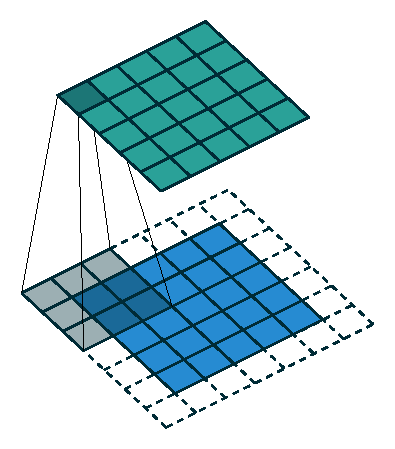
\includegraphics[width=0.24\textwidth]{figures/main/ch2-background/conv_00.pdf}
    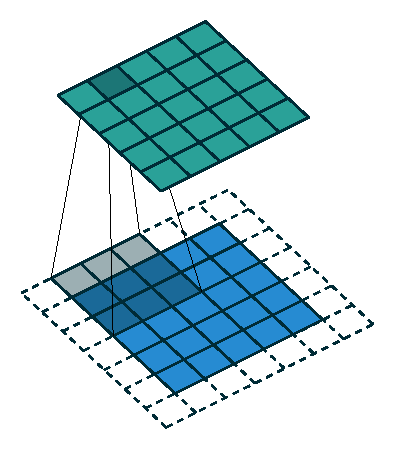
\includegraphics[width=0.24\textwidth]{figures/main/ch2-background/conv_01.pdf}
    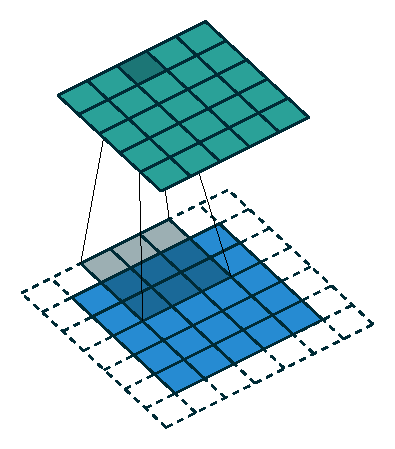
\includegraphics[width=0.24\textwidth]{figures/main/ch2-background/conv_02.pdf}
    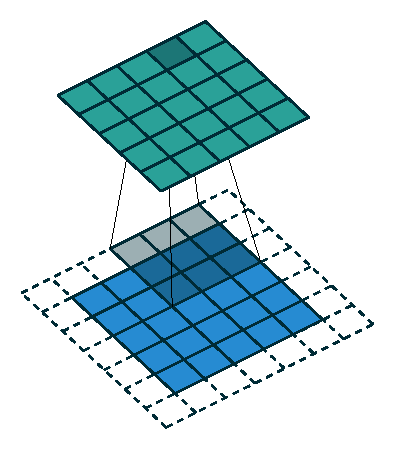
\includegraphics[width=0.24\textwidth]{figures/main/ch2-background/conv_03.pdf}
    \caption{A convolution: a kernel sliding over an image and acting as a filter. \\Illustration taken from~\citet{dumoulin2016guide}}
    \label{figure:illustration_convolution}
\end{figure}



% This observation has been made by~\citet{jain1989fundamentals} and many works have been derived from it~\citet{appuswamy2016structured,wang2020orthogonal,sedghi2018singular,singla2019bounding}, including one of our main contributions presented in \Cref{chapter:ch5-lipschitz_bound}.

A discrete convolution operation with a 2-dimensional kernel applied on a 2-dimensional signal is equivalent to a matrix multiplication with a doubly-block Toeplitz matrix.
Let $\Kmat$ be a 2-dimensional kernel defined as follows:
\begin{equation*}
  \Kmat = \leftmatrix
    k_0 & k_1 & k_2 \\
    k_3 & k_4 & k_5 \\
    k_6 & k_7 & k_8 
  \rightmatrix
\end{equation*}
then, the doubly-block Toeplitz matrix $\Mmat$ that performs the convolution can be represented as:
\begin{equation*}
  \Mmat = \leftmatrix
    \Tmat_0 & \Tmat_1 &         &         & 0       \\
    \Tmat_2 & \Tmat_0 & \Tmat_1 &         &         \\
            & \Tmat_2 & \ddots  & \ddots  &         \\
            &         & \ddots  & \Tmat_0 & \Tmat_1 \\
    0       &         &         & \Tmat_2 & \Tmat_0
  \rightmatrix
\end{equation*}
where $\Tmat_j$ are banded-Toeplitz matrices and the values of the kernel are distributed in the Toeplitz blocks as follows:
\begin{equation*}
  \Tmat_0 = \leftmatrixsmall
    k_4 & k_3 &         &         & 0       \\
    k_5 & k_4 & k_3 &         &         \\
            & k_5 & \smallddots  & \smallddots  &         \\
            &         & \smallddots  & k_4 & k_3 \\
    0       &         &         & k_5 & k_4
  \rightmatrixsmall \quad 
  \hfill
  \Tmat_1 = \leftmatrixsmall
    k_7 & k_6 &         &         & 0       \\
    k_8 & k_7 & k_6 &         &         \\
            & k_8 & \smallddots  & \smallddots  &         \\
            &         & \smallddots  & k_7 & k_6 \\
    0       &         &         & k_8 & k_7 \\
  \rightmatrixsmall \quad
  \hfill
  \Tmat_2 = \leftmatrixsmall
    k_1 & k_0 &         &         & 0       \\
    k_2 & k_1 & k_0 &         &         \\
            & k_2 & \smallddots  & \smallddots  &         \\
            &         & \smallddots  & k_1 & k_0 \\
    0       &         &         & k_2 & k_1 \\
  \rightmatrixsmall
\end{equation*}


However, in practice, the signal can have multiple channel called feature maps (\eg images have 3 channels corresponding to the color Red, Green and Blue).
Let us denote by $\cin$ and $\cout$ the number of feature maps of the input and output respectively.
Then the convolution operation takes an input of size $\cin \times n \times n$, is performed by a kernel of size $\cout \times \cin \times k \times k$ and the output signal will be of size $\cout \times m \times m$ with $m = n - k + 2p + 1$ where $p$ corresponds to the padding.
The matrix for the multi-channel convolution is the concatenation of $\cout \cdot \cin$ doubly-block Toeplitz matrices.



%%%%%%%%%%%%%%%%%%%%%%%%%%%%%%%%%%%%%%%%%%%%%%%%%%%%%%%%%%%%%%%%%%%%%%%%%%%%%%%%
\section{Summary of the Chapter}
\label{section:ch2-summary_of_the_background}
%%%%%%%%%%%%%%%%%%%%%%%%%%%%%%%%%%%%%%%%%%%%%%%%%%%%%%%%%%%%%%%%%%%%%%%%%%%%%%%%

As explained in the Introduction (\Cref{chapter:ch1-introduction}), our contributions lie at the intersection between neural networks and structured matrices.
In this chapter, we have reviewed the necessary concepts to present our contributions and some related work.

First, in \Cref{section:ch2-introduction_on_supervised_learning}, we gave a quick overview of the concept of supervised learning, which presents the mathematical tools for optimizing a parameterized function in order to map an input to an output based on a series of input-output pairs. 
Although the statistical learning framework considers generic hypothesis space, in this work we use a class of function called neural networks presented in \Cref{section:ch2-preliminaries_on_neural_networks}.
We also present, in \Cref{section:ch2-preliminaries_on_adversarial_attacks}, the concept of adversarial attacks and robustness of neural networks.
We show how a neural network can be sensitive to small perturbations to its input and thus vulnerable to adversarial examples.
Reducing the sensitivity and therefore increasing the robustness of neural networks is the central theme of our second contribution presented in \Cref{chapter:ch5-lipschitz_bound}.

Finally, \Cref{section:ch2-a_primer_on_toeplitz_and_circulant_matrices} introduce Toeplitz and Circulant matrices which are the main mathematical objects used in this thesis.
Toeplitz and circulant matrices are structured matrices in which each descending diagonal, from left to right, is constant.
The specific structured of these matrices allows linear transforms to be represented with fewer than $n^2$ parameters, which allows the construction of compact neural networks (contribution of \Cref{chapter:ch4-diagonal_circulant_neural_network}) and enables fast approximation of the Lipschitz constant of convolutional layers leading to a new regularization scheme (contribution of \Cref{chapter:ch5-lipschitz_bound}).









  %%%%%%%%%%%%%%%%%%%%%%%%%%%%%%%%%%%%%%%%%%%%%%%%%%%%%%%%%%%%%%%%%%%%%%%%%%%%%%%%
\chapter{Related Work}
\label{chapter:ch3-related_work}
%%%%%%%%%%%%%%%%%%%%%%%%%%%%%%%%%%%%%%%%%%%%%%%%%%%%%%%%%%%%%%%%%%%%%%%%%%%%%%%%
\localtoc

\section*{}

% This thesis makes contributions on building compact and robust neural networks with help from Toeplitz matrix theory.
This chapter, divided into two parts, is intended to provide an overview of the state of the art related to our contributions.
First, we present current methods for building compact neural networks.
Since the scope of application of these techniques is broad, we have chosen to focus mainly on work that uses linear algebra tools and more particularly structured matrices. 
We present in the first subsection an overview of general techniques for building compact neural networks.
In the next subsection, we present in more detail the current methods for building compact neural networks with structured matrices.
Finally, we discuss these techniques with respect to our contribution to compact neural networks.

The second part of this chapter presents current methods for regularizing the Lipschitz constant of neural networks with the aim of improving their robustness.
This section is divided into four parts.
First, we present techniques that focus on the computation of the Lipschitz constant of neural networks.
Although theoretically and empirically interesting, we will see how these techniques do not scale and therefore cannot be applied to current neural network architectures.
The following subsection presents the approach of Lipschitz regularization via the Lipschitz constant of individual layers of the networks.
We describe the advantages and disadvantages of this approach.
Moreover, in the third subsection, we focus our presentation on current techniques that compute the singular values of convolutional layers.
Finally, we discuss these techniques with respect to our contribution on Lipschitz regularization on convolutional neural networks.



% Our second contribution focuses on building robust neural networks by regularizing the Lipschitz constant of neural networks.
% Hence, we present in a second part recent works on regularizing the Lipschitz constant of neural networks.

% The second part of this chapter presents current methods for regularizing this constant that aim at improving the robustness of neural networks.
% We omit methods that are orthogonal to our approach for clarity and conciseness.


%%%%%%%%%%%%%%%%%%%%%%%%%%%%%%%%%%%%%%%%%%%%%%%%%%%%%%%%%%%%%%%%%%%%%%%%%%%%%%%%
\section{Related Work on Compact Neural Networks}
\label{section:ch3-related_work_on_compact_neural_networks}
%%%%%%%%%%%%%%%%%%%%%%%%%%%%%%%%%%%%%%%%%%%%%%%%%%%%%%%%%%%%%%%%%%%%%%%%%%%%%%%%

% In this chapter, we review the literature on techniques for building compact neural networks.
% First of all, we present, in detail, related work which uses tools from linear algebra and structured matrices. 
% Finally, we present in a more concise way concurrent techniques like using specific memory representation or using neural architecture search.
% These techniques are mostly orthogonal to our contributions.


% We have seen in the Introduction (\Cref{chapter:ch2-introduction}) and Background (\Cref{chapter:ch2-background}) that neural networks tend to be over-parametrized which lead to difficult and expensive training and overfitting.


% In this section, we review the literature for building compact neural networks.
% As seen in the Introduction (\Cref{chapter:ch1-introduction}) and Background (\Cref{chapter:ch2-background}), scaling up networks can lead to an increase in accuracy.
% Researchers have demonstrated that increasing the width of shallow neural networks increased their performance~\cite{howard2017mobilenets,sandler2018mobilenetv2,tan2019mnasnet,zagoruyko2016wide} due to their capacity to capture more fine-grained features.
% Increasing depth is a common and effective way to scale neural networks and many deep architectures have been proposed~\cite{he2016deep, huang2016deep, szegedy2016rethinking,szegedy2017inception,xiao2018dynamical}. 
% The intuition is that deep neural network can capture richer and more complex features.


% Increasing the width of shallow neural networks can increase their performance~\cite{howard2017mobilenets,sandler2018mobilenetv2,tan2019mnasnet,zagoruyko2016wide} due to their capacity to capture more fine-grained features.
% As well, increasing depth is a common and effective approach to capture richer and more complex features and increase performance, many deep architectures have been proposed~\cite{he2016deep,huang2016deep, szegedy2016rethinking,szegedy2017inception,xiao2018dynamical}.
% However, large neural networks lead to difficult and expensive training and overfitting and after observing that a lot of parameters in large neural networks were redundant~\cite{dai2018compressing,frankle2018lottery}, an important question arises: \emph{do neural networks needs to be over-parameterized? And if not, how to build accurate and compact neural networks?} 

%%%%%%%%%%%%%%%%%%%%%%%%%%%%%%%%%%%%%%%%%%%%%%%%%%%%%%%%%%%%%%%%%%%%%%%%%%%%%%%%
\subsection{General Techniques to Build Compact Neural Networks}
%%%%%%%%%%%%%%%%%%%%%%%%%%%%%%%%%%%%%%%%%%%%%%%%%%%%%%%%%%%%%%%%%%%%%%%%%%%%%%%%

As seen in the Introduction (\Cref{chapter:ch1-introduction}), scaling up networks can lead to better accuracy~\cite{tan2019efficientnet,brown2020language}.
However, large neural networks lead to difficult and expensive training and after observing that a lot of parameters in large neural networks were redundant~\cite{dai2018compressing,frankle2018lottery}, an important question arises: \emph{do neural networks need to be over-parameterized? And if not, how to build accurate and compact neural networks?} 

Numerous other directions have been investigated to build compact and cost-effective neural networks without impacting the accuracy.
For example \citet{gupta2015deep,micikevicius2018mixed} have proposed to represent weights with limited numerical precision to reduce training time and memory requirements.
They used half-precision floating-point format instead of single-precision floating-point format which uses 32 bits of computer memory.
In the same direction, \citet{courbariaux2015binaryconnect} have proposed a method to train neural networks with binary weights without an important loss in the accuracy.

An important idea in model compression, proposed by~\citet{bucilua2006model}, is based on the observation that the model used for training is not required to be the same as the one used for inference.
Indeed, compressed models after training can be deployed on smartphones or IoT devices.
Based on this idea, multiple post-processing techniques have been developed: a quantization procedure which consists in converting the weights into a binary or integer formats \emph{after} the training phase~\cite{mellempudi2017ternary,rastegariECCV16}, pruning techniques~\cite{dai2018compressing,han2015deep,lin2017runtime} or sparsity regularizers~\cite{collins2014memory,dai2018compressing,liu2015sparse} which consists in removing redundant weights after training and taking advantage of the sparse structure of the weight matrices.

Sparse neural networks have also been extensively studied since the seminal work of \citet{frankle2018lottery} in which they propose the \emph{Lottery Ticket Hypothesis}. 
This hypothesis states that there exists a sparse subnetwork of a dense neural network that when trained in isolation can match the test accuracy of the original dense network after training for at most the same number of iterations. 
This hypothesis led to a series of works on sparse neural networks \cite{zhou2019deconstructing,malach2019proving,evci2020rigging}.

Moreover, \citet{ba2014deep} have empirically demonstrated that shallow neural networks can learn the complex functions previously learned by other deep neural networks.
This result led \citet{hinton2015distilling} to propose a technique called \emph{model distillation} which consists in training a large complex model using all the available data and resources to be as accurate as possible, then a smaller and more compact model is trained to approximate the first model.
Although interesting for deployment purposes, this approach still requires to train one large network and one shallow, which entails a significant training cost.

\begin{figure}[t]
  \centering
  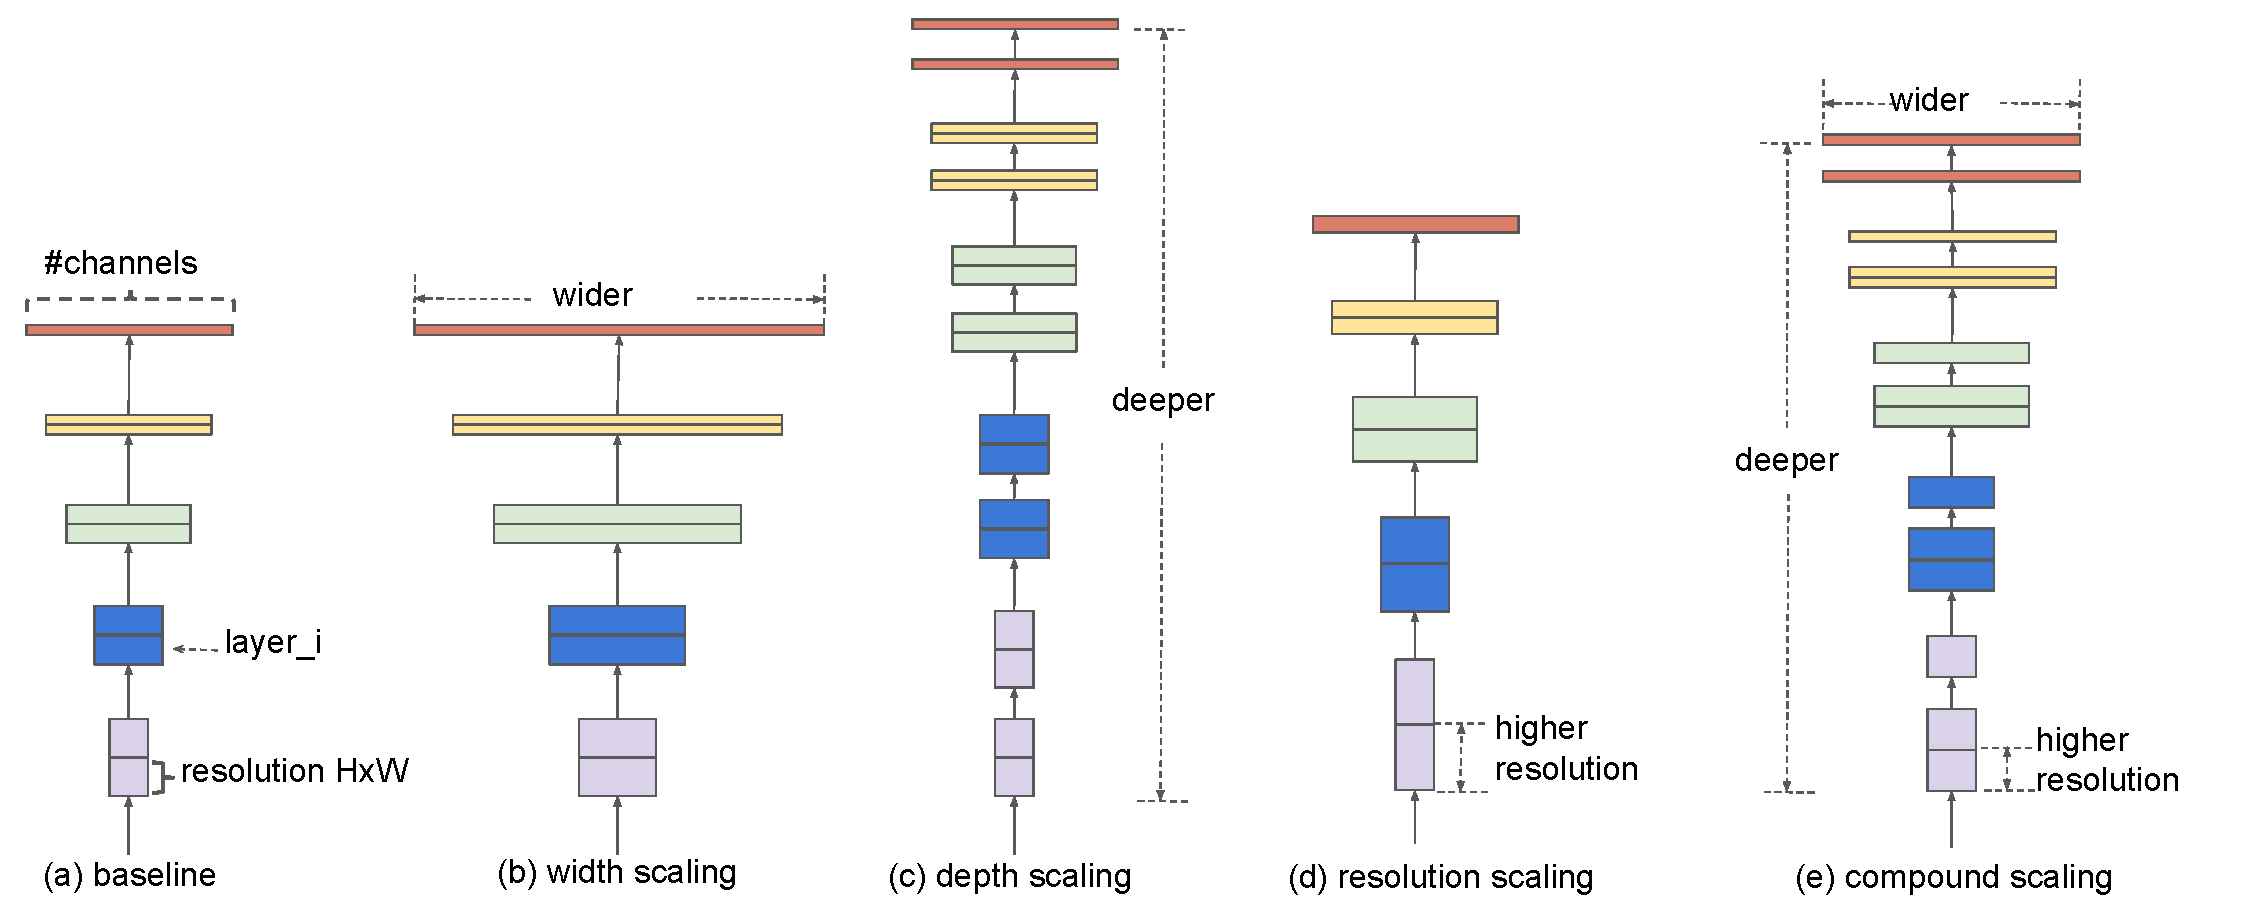
\includegraphics[width=0.80\textwidth]{figures/main/ch3-related_work/scalecompare.pdf}
  \caption{Illustration of the scaling of the EfficientNet architecture.}
  \label{figure:p1-ch3-illustration_efficientnet}
\end{figure}

More recently, \citet{zoph2018learning,real2019regularized} have designed algorithms that automatically tune the width and depth of neural network architectures to obtain the best trade-off between compactness and accuracy.
With this approach, \citet{tan2019efficientnet} found a new compound scaling method that uniformly scales network width and depth leading to efficient and compact architecture.
\Cref{figure:p1-ch3-illustration_efficientnet} illustrates the different scaling proposed by~\citet{tan2019efficientnet}.

% Finally, in the context of deep learning, compact representations have gained much attention over the past years as a way to compress models or to reduce memory requirements.
% In this thesis, we focus on building compact neural networks with structured matrices.
% Hereafter, we present a comprehensive overview of the existing techniques in this line of research.



% --> Compact Neural Networks Architecture

% Without consideration of specific memory representations, data structures or structured linear layers, it is still possible to design compact neural networks.
%
% However, researchers have demonstrated that increasing the width of shallow neural networks increased their performance~\cite{howard2017mobilenets,sandler2018mobilenetv2,tan2019mnasnet,zagoruyko2016wide} due to their capacity to capture more fine-grained features.
% Finally, depth is a common and effective way to scale neural networks and many deep architectures have been proposed~\cite{he2016deep, huang2016deep, szegedy2016rethinking,szegedy2017inception,xiao2018dynamical}. 
% The intuition is that deep neural network can capture richer and more complex features.
%
% After observing that large and deep neural networks outperformed shallow ones \cite{huang2019gpipe,brown2020language} and the observation that a lot of parameters in large neural networks were redundant~\cite{dai2018compressing,frankle2018lottery}, an important question arises: \emph{do neural networks needs to be large \ie, deep and wide, and if not, which architecture provides the best accuracy?} 

% \citet{ba2014deep} tried to answer this question and empirically demonstrated that shallow neural networks can learn the complex functions previously learned by another neural network. 
% This observation was then leveraged by~\citet{hinton2015distilling} for compressing trained neural networks.
% Their technique, called \emph{model distillation}, consists to train a large complex model using all the available data and resources to be as accurate as possible, then a smaller and more compact model is trained to approximate the first model.
% Although, this approach can be interesting for deployment purposes, it is still required to train one large network and one shallow, which entails a significant training cost.
%
% Instead of compressing the model after the training step, researchers still tried to design architectures that are compact by nature but finding the best trade-off between depth, width and performance has proved to be a tedious work.
% In order to scale the search, recent works have devised algorithms to automatically find the best architecture for a specific use case.
% \citet{zoph2018learning,real2019regularized} have tried to tune the wide and depth of neural network architectures to obtain the best trade-off between efficiency and accuracy but these methods required a lot of manual tuning.
% More recently, with a similar method, \citet{tan2019efficientnet} found a new compound scaling method to uniformly scales network width, depth, and resolution leading to groundbreaking result in terms of efficiency and accuracy.




%%%%%%%%%%%%%%%%%%%%%%%%%%%%%%%%%%%%%%%%%%%%%%%%%%%%%%%%%%%%%%%%%%%%%%%%%%%%%%%%
\subsection{Building Compact Neural Networks with Structured Matrices}
\label{subsection:ch3-building_compact_neural_networks_with_structured_matrices}
%%%%%%%%%%%%%%%%%%%%%%%%%%%%%%%%%%%%%%%%%%%%%%%%%%%%%%%%%%%%%%%%%%%%%%%%%%%%%%%%

% An effective method to build compact neural networks is to constrain the hypothesis space in which the learning algorithm ``chooses'' the predictor.
% As seen in \Cref{chapter:ch2-background}, this constraint is called \emph{inductive bias}. 

% Another way of constraining the weight representation and reduce the memory requirement of neural networks is to impose a \emph{structure} on weight matrices. 

% The idea of building compact neural networks with structured matrices consists of replacing the weight matrices $\Wmat^{(i)}$ with \emph{structured matrices}.


% A structured matrix is a $n \times n$ matrix whose entries have a formulaic relationship, allowing the matrix to be represented with fewer than $n^2$ parameters.
% The formulaic relationship between entries is an important feature to consider, for example, a sparse matrix has fewer than $n^2$ parameters but does not have a clear relationship between its entries.

% by using \emph{structured neural networks}. 
% The idea of structured neural networks consists of replacing the dense weight matrices with \emph{structured} ones.

An effective method to build compact neural networks is to constrain the hypothesis space by imposing a \emph{structure} on the weight matrices which constitute the different layers of the network.
% A structured matrix is a $n \times n$ matrix which can be represented with fewer than $n^2$ parameters and where the entries are distributed along specific rules.

%%%%%%%%%%%%%%%%%%%%%%%%%%%%%%%%%%%%%%%%%%%%%%%%%%%%%%%%%%%%%%%%%%%%%%%%%%%%%%%%
\paragraph{Structured Neural Networks with Low Rank Approximation} ~\\
%%%%%%%%%%%%%%%%%%%%%%%%%%%%%%%%%%%%%%%%%%%%%%%%%%%%%%%%%%%%%%%%%%%%%%%%%%%%%%%%

\noindent
For example, \citet{sainath2013lowrank} were among the first to use low-rank matrices in deep learning contexts followed by the work of~\citet{jaderberg2014speeding,yu2017compressing}.
Their work consists in replacing the weight matrices of size $n \times m$ by the product of two rectangular matrices of size $n \times r$ and $r \times m$, where $r$ corresponds to the rank of the new matrix. 
In order to reduce the number of parameters, the rank $r$ is chosen to be small such that $r \ll \min(m, n)$.
By representing the weight matrices with a low-rank decomposition, one can reduce the storage from $mn$ parameters to $(mr + nr)$ and accelerate the matrix-vector product from $\bigO(mn)$ to $\bigO(mr + rn)$.
To enforce the low-rank constraint, reduced storage and computation time during training, the authors trained the coefficients of the two rectangular matrices directly. 
Formally, let $\Wmat \in \Rbb^{n \times m}$ be a weight matrix and let $\widetilde{\Wmat}$ be the low-rank approximation of rank $r$ of the matrix $\Wmat$.
Then, the low-matrix $\widetilde{\Wmat}$ can be decomposed by the product of two rectangular matrices $\Umat \in \Rbb^{n \times r}$ and $\Vmat \in \Rbb^{r \times m}$ such that $\widetilde{\Wmat} = \Umat \Vmat$.
Therefore, a neural network layer with low-rank approximation can be expressed as follows:
\begin{equation}
  \layer_{\Umat, \Vmat, \bvec} (\xvec) = \act\left( \Umat \Vmat \xvec + \bvec \right) .
\end{equation}
The scalar $r$ defining the size of the two rectangular matrices becomes an hyper-parameter and controls the trade-off between the expressivity and compactness of the layer. 

In the same vein, \citet{oseledets2011tensor} have proposed the \emph{Tensor Train decomposition} (TT-decomposition), which is based on the tensor rank decomposition (Tucker decomposition) proposed by~\citet{hitchcock1927expression} and named after \citet{tucker1966some}.
The TT-decomposition is defined as follows.
Let $\boldsymbol{\Aset} \in \Rbb^{n_1 \times n_2 \times \dots \times n_{d-1} \times n_d}$ be a $d$-dimensional tensor.
The Tensor-Train Decomposition factorizes $\boldsymbol{\Aset}$ in a product of third-order tensors and it is given by: 
\begin{equation}
  (\boldsymbol{\Aset})_{(i_1,\dots,i_d)} = (\Gmat^{(1)})_{(i_1, :)} (\boldsymbol{\Gset}^{(2)})_{(:, i_2, :)} (\boldsymbol{\Gset}^{(3)})_{(:, i_3, :)} \dots (\Gmat^{(d)})_{(:, i_d)}
\end{equation}
where $\Gmat^{(i)}$ are matrices and $\boldsymbol{\Gset}^{(i)}$ are third-order tensors of size $r_{i} \times r_{i+1}$ called \emph{TT-cores}.
The sequence $\{r_k\}_{k=0}^d$ is referred to as the ranks of the TT-representation.
The above equation can be equivalently rewritten as a sum of elements of the TT-cores:
\begin{equation}
  (\boldsymbol{\Aset})_{(i_1,\dots,i_d)} = \sum_{\alpha_1, \dots, \alpha_{d-1}} (\Gmat^{(1)})_{(i_1, \alpha_1)} (\boldsymbol{\Gset}^{(2)})_{(\alpha_1, i_2, \alpha_2)} \dots (\Gmat^{(d)})_{(\alpha_{d-1}, i_d)}
\end{equation}
\citet{oseledets2011tensor} have shown that for an arbitrary tensor $\boldsymbol{\Aset}$, several TT-representations exist with different ranks.
The TT-decomposition can be very efficient in terms of memory requirement if the ranks are small.
Indeed, the tensor $\boldsymbol{\Aset}$ has $\prod_{k=1}^{d} n_k$ values compared with $\sum_{k=1}^d n_k r_{k-1} r_k$ values.

The TT-decomposition has been extensively used in the context of deep learning.
\citet{novikov2015tensorizing} was one of the first to use this technique to reduce the number of parameters of neural networks by using the decomposition to replace the fully connected layer of the VGG architecture~\cite{simonyan2014very}.
They reported a compression factor of the dense weight matrix up to 200000 times leading to the compression factor of the whole network up to 7 times with only 0.3 point drop of TOP-5 accuracy on ImageNet~\cite{deng2009imagenet}.
With this work, \citet{novikov2015tensorizing} have demonstrated that the TT-decomposition allows an important reduction of the number of parameters while preserving the expressive power of the layers.
Later, the TT-decomposition was used in other types of architectures.
\citet{garipov16ttconv} used it to compress convolutional layers as well as fully connected layers.
\citet{yang2017tensor} used it in the context of video classification, \citet{tjandra2017compressing} compressed the layers of recurrent neural networks and finally, \citet{xindian2019tensorized} developed a compact architecture based on TT-decomposition for Language Modeling.

However, the Tensor-Train decomposition has some limitations.
Although it can reduce the number of parameters when the ranks are low, finding the best alignment of the tensor dimensions in order to find the best optimized TT-cores remains a challenging problem, as stated by~\citet{pan2019compressing}.


% In the same vein, \citet{novikov2015tensorizing} have proposed a generalization of low-rank decomposition.
% Instead of searching for low-rank approximation of the weight matrices, they consider multi-dimensional tensors and apply the \emph{Tensor Train decomposition} algorithm \cite{oseledets2011tensor}.
% The Tensor Train decomposition allows an important reduction of the number of parameters while preserving the expressive power of the layers.



%%%%%%%%%%%%%%%%%%%%%%%%%%%%%%%%%%%%%%%%%%%%%%%%%%%%%%%%%%%%%%%%%%%%%%%%%%%%%%%%
\paragraph{Neural Networks with Diagonal and Circulant Matrices} ~\\
%%%%%%%%%%%%%%%%%%%%%%%%%%%%%%%%%%%%%%%%%%%%%%%%%%%%%%%%%%%%%%%%%%%%%%%%%%%%%%%%

\noindent

% Since the seminal work of \citet{ailon2009fast}, structured transforms have been extensively studied in the context of dimensionality reduction and random projections.
% For example, the Fastfood transform which was proposed by \cite{le2013fastfood}  
%
% Other types of structured transforms have been used to  


% The authors have replaced dense matrices of fully connected layers with adaptive structured matrices of the form: $\Smat\Hmat\Gmat\mathbf{\Pi}\Hmat\Bmat$ where $\Smat$, $\Gmat$, and $\Bmat$ are adaptive diagonal matrices, $\mathbf{\Pi}$ is a random permutation matrix, and $\Hmat$ is the Walsh-Hadamard matrix.


% Other types of decomposition have been used to reduce the number of parameters of neural networks.
% The Fastfood transform which was originally used for approximating kernel expansions~\cite{le2013fastfood}, was later used in neural networks by~\citet{yang2015deep} leading to the Deep Fried Convnets architecture.
% The authors have replaced dense matrices of fully connected layers with adaptive structured matrices of the form: $\Smat\Hmat\Gmat\mathbf{\Pi}\Hmat\Bmat$ where $\Smat$, $\Gmat$, and $\Bmat$ are adaptive diagonal matrices, $\mathbf{\Pi}$ is a random permutation matrix, and $\Hmat$ is the Walsh-Hadamard matrix.
% Later, the \emph{Structured Spinners} transform of the form: $\Hmat\Dmat^{(3)} \Hmat\Dmat^{(2)} \Hmat\Dmat^{(1)}$, where $\Hmat$ is the Walsh-Hadamard matrix, and $\Dmat^{(i)}$ for $i \in {1, 2, 3}$ is a random $\pm1$-diagonal matrix, was originally proposed by~\citet{andoni2015practical} and used in deep learning settings by~\citet{bojarski2017structured}.



% Key to Fastfood is the observation that Hadamard 
% matrices when combined with diagonal Gaussian
% matrices exhibit properties similar to dense
% Gaussian random matrices. Yet unlike the
% latter, Hadamard and diagonal matrices are
% inexpensive to multiply and store.

% which can be viewed as a generalized class of Fourier transforms.

% Decomposition with structured matrices of interest for the contributions of this thesis are the ones based on diagonal and circulant matrices.

% More practically, \citet{hinrichs2011johnson} have shown that the \DC transform $\xvec \mapsto \Dmat \Cmat \xvec$, where the matrix $\Dmat$ is a diagonal matrix with entries sampled from $\{1, -1\}$ and $\Cmat$ is a circulant matrix based on a sequence of independent identically distributed random variables respect the \citeauthor{johnson1984extensions} lemma.
\citet{cheng2015exploration} proposed to replace the weight matrix of a fully connected layer by the product of a circulant and a diagonal matrix leading to following structured layer:
\begin{equation}
  \layer_{\Dmat, \Cmat, \bvec} (\xvec) = \act \left( \Dmat \Cmat \xvec + \bvec \right) \enspace,
\end{equation}
where the circulant matrix is learned by a gradient-based optimization algorithm and the diagonal matrix entries are sampled at random in $\{-1, 1\}$. 
The idea of replacing dense matrices with circulant ones comes from their use in dimensionality reduction with the \emph{fast Johnson-Lindenstrauss transform}~\cite{hinrichs2011johnson,vybiral2011variant}, binary embedding~\cite{yu2014circulant}, and kernel approximation~\cite{yu2015compact}, etc.
Circulant matrices exhibit several interesting properties from the perspective of numerical computations.
Recall from \Cref{theorem:ch2-diagonalization_circulant_matrix} that circulant matrices can be diagonalized with the Fourier Transform as follows:
\begin{equation}
  \Cmat = \frac{1}{n} \Umat_n^* \diag(\Umat_n \cvec) \Umat_n \enspace.
\end{equation}
where the vector $\cvec$ corresponds to the first columns of the matrix $\Cmat$.
This decomposition allows a compact representation in memory ($n$ values instead of $n^2$) and efficient matrix-vector product with the FFT algorithm (see \Cref{algorithm:ch2-matrix_vector_product_circulant_matrix}).
% Thanks to this decomposition, circulant matrices exhibit several interesting properties from the perspective of numerical computations. Most importantly, any $n \times n$ circulant matrix $\Cmat$ can be represented using only $n$ coefficients instead of the $n^2$ coefficients required to represent classical unstructured. In addition, the matrix-vector product is simplified from O(n 2) to O(n log(n)) using the convolution theorem.
% Thanks to this decomposition, circulant matrices offer a compact representation in memory (they can be expressed with only $n$ values instead of $n^2$) and an efficient matrix-vector product with the FFT algorithm (see \Cref{algorithm:ch2-matrix_vector_product_circulant_matrix}).
Despite the reduction of expressivity, \citet{cheng2015exploration} demonstrated good empirical results using only a fraction of the original weights (90\% reduction). 


\citet{moczulski2016acdc} built upon the work of~\citet{cheng2015exploration} and \citet{huhtanen2015factoring} and introduced two \emph{Structured Efficient Linear Layers} (SELL) based on the Fourier and cosine transforms.
First, by observing that the DC transform cannot express an arbitrary linear operator they proposed to apply the result of \citet{huhtanen2015factoring} which states that almost all matrices can be decomposed as a product of DC transforms.
\begin{theorem}[Reformulation from \citet{huhtanen2015factoring}] \label{theorem:ch3-huhtanen}
  For every matrix $\Mmat \in \Cbb^{n \times n}$, for any $\epsilon > 0$, there exists a sequence of matrices $\{ \Amat^{(i)} \}_{i \in [2n-1]}$ where $\Amat^{(i)}$ is a circulant matrix if $i$ is odd, and a diagonal matrix otherwise, such that $\norm{\Amat^{(1)} \ldots \Amat^{(2n-1)} - \Mmat} < \epsilon$.
\end{theorem}
\noindent
Based on this result, they proposed to parameterize the layers of a neural network with $k$ products of diagonal and circulant matrices as follows:
\begin{equation} \label{equation:acdc_layer}
  \layer_{\Dmat, \Cmat, \bvec} (\xvec) = \act \left( \left(\prod_{i = 1}^{k} \Dmat^{(i)} \Cmat^{(i)} \right) \xvec + \bvec \right)
\end{equation}
where $\Dmat$ and $\Cmat$ are sequences of $k$ diagonal and circulant matrices respectively.
This structured layer is therefore parameterized by $n(2k+1)$ values and the value $k$ becomes a hyper-parameter controlling the trade-off between compactness and expressivity. 
By diagonalizing the circulant matrix, the layer in \Cref{equation:acdc_layer} can be expressed as a product of diagonal matrices and the Fourier transform as follows:
\begin{equation} \label{equation:ch3-laye_acdc}
  \layer^\act_{\dvec, \cvec, \bvec} (\xvec) = \act \left(\frac{1}{n^k} \left(\prod_{i = 1}^{k} \diag\left(\dvec^{(i)}\right) \Umat_n^* \diag\left(\Umat_n \cvec^{(i)}\right) \Umat_n \right) \xvec + \bvec \right)
\end{equation}
\noindent
Although interesting and demonstrating good empirical results, the work of~\citet{moczulski2016acdc} suffers from multiple limitations. 
First, the result from~\citet{huhtanen2015factoring} is expressed with respect to $n$, the size of the matrices $\Amat$.
Therefore, the theorem does not provide any insights regarding the expressive power of $k$ factors when $k$ is much lower than $2n-1$ as it is the case in most practical scenarios they consider.
Finally, in order to stay in the real domain, they replaced the Fourier transform in~\Cref{equation:ch3-laye_acdc} with the cosine transform thus learning a different kind of linear transform (see the work of~\citet{sanchez1995diagonalizing} which characterizes the matrices diagonalizable by the cosine transform).
Furthermore, because the cosine transform does not diagonalize circulant matrices, \Cref{theorem:ch3-huhtanen} no longer applies.


% \vspace{0.3cm}

%%%%%%%%%%%%%%%%%%%%%%%%%%%%%%%%%%%%%%%%%%%%%%%%%%%%%%%%%%%%%%%%%%%%%%%%%%%%%%%%
\paragraph{General Representation of Structured Linear Maps: LDR and K-Matrices} ~\\
%%%%%%%%%%%%%%%%%%%%%%%%%%%%%%%%%%%%%%%%%%%%%%%%%%%%%%%%%%%%%%%%%%%%%%%%%%%%%%%%

\vspace{-0.5cm}

General framework for structured matrices that reduce the memory footprint but also accelerate matrix-vector product operations have been used to build compact neural networks.
\citet{sindhwani2015structured} have used the notion of low displacement rank presented in \Cref{subsection:ch2-general_frameworks_for_structured_matrices} to learn a broad family of structured matrices.
Recall from~\Cref{theorem:ch2-toeplitz_like} that all matrices expressed as the following sum of products are called \emph{Toeplitz-like} matrices:
\begin{equation}
    \Mmat = \sum_{j=1}^{r} \Zmat_1(\gvec^{(j)}) \Zmat_{-1}(\Jmat_n \hvec^{(j)})
\end{equation}
where $\Zmat_f$ is an $f$-circulant matrix defined in \Cref{definition:ch2-f_circulant_matrix} and $\Gmat = \leftmat \gvec^{(1)} \ldots \gvec^{(r)} \rightmat, \Hmat = \leftmat \hvec^{(1)} \ldots \hvec^{(r)} \rightmat \in \Rbb^{n \times r}$ with $r \ll n$.
More precisely, \citet{sindhwani2015structured} proposed to learn Toeplitz-like matrices by learning the factors $\Gmat$ and $\Hmat$. 
Therefore, they proposed the following parameterized layer:
\begin{equation}
  \layer_{\Gmat, \Hmat, \bvec}(\xvec) = \act \left( \left(\sum_{j=1}^{r} \Zmat_1\left(\gvec^{(j)}\right) \Zmat_{-1}\left(\Jmat_n \hvec^{(j)}\right) \right) \xvec + \bvec \right)
\end{equation}
where the rank $r$ is a hyper-parameter and controls the number of parameters of the layer.
In addition to offer fast matrix-vector product, they have showed that this class of layers is very rich from a modeling perspective.
More precisely, they characterize the expressivity of the layer as follows: 
\begin{theorem}[LDR expressivity \citet{pan2001structured,sindhwani2015structured}] ~\\
  The set of all $n \times n$ matrices that can be written as, $\sum_{i=1}^{r} \Zmat_1(\gvec^{(i)}) \Zmat_{-1}(\hvec^{(i)})$
  for some $\Gmat = \leftmat \gvec^{(1)} \ldots \gvec^{(r)} \rightmat,
  \Hmat = \leftmat \hvec^{(1)} \ldots \hvec^{(r)} \rightmat \in \Rbb^{n \times r}$ contains:
  \begin{compactitem}
    \item All $n \times n$ Circulant and Skew-Circulant matrices for $r \geq 1$.
    \item All $n \times n$ Toeplitz matrices for $r \geq 2$.
    \item Inverses of Toeplitz matrices for $r \geq 2$.
    \item All products of the form $\Amat^{(1)} \ldots \Amat^{(t)}$ for any $t \leq \frac{r}{2}$.
    \item All linear combinations of the form $\sum_{i=1}^p \beta_i \Amat^{(1, i)} \ldots \Amat^{(t, i)}$ for any $t \leq \frac{r}{2p}$.
    \item All $n\times n$ matrices for $r=n$.
  \end{compactitem}
  where each $\Amat^{(i)}$ above is a Toeplitz matrix or the inverse of a Toeplitz matrix. 
\end{theorem}
\noindent

In the same line of work, \citet{thomas2018learning} have proposed neural network layers directly form the Krylov decomposition presented in~\Cref{theorem:ch2-krylov_decomposition} which encompasses an even larger family of structured matrices including Toeplitz-like, Vandermonde-like, Cauchy-like ones.
Despite being elegant and general, we found that the LDR framework suffers from several limits which are inherent to its generality and makes it difficult to use in the context of deep neural networks.
% First, the training procedure for learning LDR matrices is highly involved and implies many complex mathematical objects such as Krylov matrices.
As acknowledged by the authors, the number of parameters required to represent a given structured matrix (a Toeplitz matrix) in practice is unnecessarily high (higher than required in theory) making the training very hard. 



More recently, another type of generalization of structured linear maps has been proposed by~\citet{dao2019learning,dao2020kaleidoscope}.
They introduced a family of matrices called \emph{kaleidoscope matrices} (K-matrices) which are the product of sparse matrices with specific predefined sparsity patterns.
They showed that this type of matrices can capture any sparse matrix with near-optimal space (parameter) and time (arithmetic operation) complexity.
The authors claim that their structured linear maps can capture more common structures with a few numbers of parameters than the displacement operators presented above.
More precisely, their representation is based on products of a particular building block known as a butterfly matrix introduced by~\citet{parker1995random}.
Butterfly matrices have been extensively used in numerical linear algebra~\cite{parker1995random,li2015butterfly} and machine learning~\cite{mathieu2014fast,jing2017tunable,munkhoeva2018quadrature,dao2019learning,choromanski2019unifying}.








%%%%%%%%%%%%%%%%%%%%%%%%%%%%%%%%%%%%%%%%%%%%%%%%%%%%%%%%%%%%%%%%%%%%%%%%%%%%%%%%
\subsection{Discussion}
%%%%%%%%%%%%%%%%%%%%%%%%%%%%%%%%%%%%%%%%%%%%%%%%%%%%%%%%%%%%%%%%%%%%%%%%%%%%%%%%

In this section, we have shown current methods and techniques for designing compact neural networks with structured matrices. 
Our contributions on \emph{Deep Diagonal Circulant Neural Networks} are a direct follow-up to the work of~\citet{cheng2015exploration,sindhwani2015structured,moczulski2016acdc,thomas2018learning} focusing on compact neural networks with \emph{structured matrices}.
More precisely, we extend the work of \citet{moczulski2016acdc} by training \emph{fully structured networks} (\ie, networks with structured layers only) hence demonstrating that diagonal circulant layers are able to model complex relations between inputs and outputs.
Although, this diagonal circulant layers fit in the low displacement rank framework, we demonstrate much better performances in practice.
Indeed, thanks to a solid theoretical analysis and thorough experiments, we were able to train deep (up to 40 layers) circulant neural networks, and apply, for the first time, this structured architecture in the context of large-scale video classification.
This contrasts with previous experiments in which only one or a few dense layers were replaced inside a large redundant network such as VGG~\cite{simonyan2014very}.

% \pagebreak

%%%%%%%%%%%%%%%%%%%%%%%%%%%%%%%%%%%%%%%%%%%%%%%%%%%%%%%%%%%%%%%%%%%%%%%%%%%%%%%%
\section{Related Work on Lipschitz Regularization}
\label{section:ch3-related_work_on_lipschitz_regularization}
%%%%%%%%%%%%%%%%%%%%%%%%%%%%%%%%%%%%%%%%%%%%%%%%%%%%%%%%%%%%%%%%%%%%%%%%%%%%%%%%

%%%%%%%%%%%%%%%%%%%%%%%%%%%%%%%%%%%%%%%%%%%%%%%%%%%%%%%%%%%%%%%%%%%%%%%%%%%%%%%%
\subsection{The Global Lipschitz Constant of Neural Networks}
\label{subsection:ch3-the_global_lipschitz_constant_of_neural_networks}
%%%%%%%%%%%%%%%%%%%%%%%%%%%%%%%%%%%%%%%%%%%%%%%%%%%%%%%%%%%%%%%%%%%%%%%%%%%%%%%%

\noindent
The regularization of the Lipschitz constant of neural networks has seen a growing interest in the training of neural networks.
Indeed, numerous results have shown that neural networks with a low Lipschitz constant exhibit better generalization~\cite{bartlett2017spectrally} and higher robustness to adversarial attacks~\cite{szegedy2013intriguing,tsuzuku2018lipschitz, farnia2018generalizable}.

The Lipschitz constant, defined in~\Cref{definition:ch2-lipschitz_constant}, is a measure of the stability of the network
If the Lipschitz constant is high, the network will tend to be more sensitive to input perturbation.
Intuitively, the Lipschitz constant $k$ of a function $f$ is a bound on the slope of $f$.
Meaning, if the input changes by $\epsilon$, the output changes by at most $k\epsilon$.
Therefore, the Lipschitz constant of a function can also be expressed using the differential operator as follows:
\begin{theorem}[Rademacher's Theorem] \label{theorem:ch3-lipschitz_differential_op}
  If $f: \Rbb^n \rightarrow \Rbb^m$ is a Lipschitz continuous function, then $f$ is differentiable almost everywhere.
  Moreover, if $f$ is Lipschitz continuous, then
  \begin{align}
    \lip{f} = \sup_{\xvec \in \Rbb^n} \norm{\mathrm{D}_\xvec f(\xvec)}_2
  \end{align}
  where $\mathrm{D}_\xvec$ is the differential operator of $f$ at $\xvec$.
\end{theorem}

\citet{tsuzuku2018lipschitz} have studied the relationship between the robustness of a neural network and the Lipschitz constant and the margin of the neural networks. 
By the definition of the Lipschitz constant, we have the following:
\begin{equation}
  \norm{N(\xvec) - N(\xvec + \adv)}_2 \leq \lip{N} \norm{\adv}_2
\end{equation}
Recall the margin operator $\Mset: \Rbb^k \times [k] \rightarrow \Rbb$ from~\Cref{subsection:ch2-recent_results_on_the_theory_of_neural_networks} defined as:
\begin{equation}
  \Mset(\vvec, j) \triangleq \vvec_j - \max_{i \neq j} \vvec_i
\end{equation}
% Let us denote the margin of the neural network $N$ with respect to the tuple $(\xvec, y)$ as follows:
% \begin{equation}
%   \mathcal{M}^{N}_{(\xvec, y)} \triangleq N(\xvec)_y - \max_{i \neq y} \left( N(\xvec) \right)_i
% \end{equation}
Then, we have the following proposition which characterize the robustness of a neural network with respect to its margin and Lipschitz constant.
\begin{proposition}[\citet{tsuzuku2018lipschitz}]
  \begin{equation} \label{equation:ch3-margin_guarded_area}
    \Mset \big( N(\xvec), y \big) \geq \sqrt{2} \lip{N} \norm{\adv}_2 \quad \Longrightarrow \quad \Mset \big( N(\xvec + \adv), y \big) \geq 0
  \end{equation}
  \removespace
\end{proposition}
\noindent
If the inequality on the right-hand side of \Cref{equation:ch3-margin_guarded_area} is verified then the adversarial margin is positive, \ie, the network correctly predicts the label. 
From this proposition, we can conclude that for a given neural network with specific margins, a lower Lipschitz constant allows for an increase in robustness. 
Note that the margin is already maximized in a multi-class setting with the cross-entropy loss as stated in~\citet{hein2017formal}.
A multitude of work have tried to reduce the Lipschitz constant in order to improve adversarial robustness.
However, \citet{scaman2018lipschitz} have shown that computing the exact Lipschitz constant of a neural network is NP-hard.
The following theorem shows that, even for shallow neural network, exact Lipschitz computation is not achievable in polynomial time:
\begin{theorem}[\citet{scaman2018lipschitz}] \label{theorem:ch3-lipschitz_computation}
  Let us define the problem associated with the exact computation of the Lipschitz constant of a $2$-layer neural network with $\relu$ activation:
  \begin{itemize}%[topsep=0pt,noitemsep]
    \item[] \textbf{Input:} Two matrices $\Wmat^{(1)} \in \Rbb^{l \times n}$ and $\Wmat^{(2)} \in \Rbb^{m \times l}$, and a constant $c \geq 0$.
    \item[] \textbf{Question:} Let $N = \Wmat^{(2)} \circ \rho \circ \Wmat^{(1)}$ where $\rho$ is the $\relu$ activation function. \emph{Is the Lipschitz constant $\lip{N} \leq c$ ?}
  \end{itemize}
  Then, assuming that $\mathbf{P} \neq \mathbf{NP}$, the problem above is \textbf{NP}-hard. 
\end{theorem}


\noindent
To overcome this difficulty, researchers have relied on devising a tight upper bound of the Lipschitz constant.
For example, \citet{scaman2018lipschitz} have shown that the Lipschitz constant of a neural network $N$ can be explicitly formulated using \Cref{theorem:ch3-lipschitz_differential_op} and the chain rule:
\begin{equation} \label{equation:ch3-decomposition_jacobian_lipschitz}
  \lip{\nn} = \sup_{x \in \Rbb^n} \norm{\Wmat^{(p)} \diag(\rho'_\depth(\theta_\depth)) \dots \Wmat^{(2)} \diag(\rho'_1(\theta_1)) \Wmat^{(1)}}_2,
\end{equation}
where $\theta_i = \layer^{\act_i}_{\Wmat^{(i)}, \bvec^{(i)}} \circ \cdots \circ \layer^{\act_1}_{\Wmat^{(1)}, \bvec^{(1)}}(\xvec)$ is the intermediate output after $i$ layers.
The Lipschitz of the neural network $N$ can then be upper bounded as follows:
\begin{align}
  \lip{\nn} &\leq \max_{\forall i,\ \sigma_i \in [0, 1]^{w^{(i+1)}}} \norm{\Wmat^{(\depth)} \diag(\sigma_{\depth-1}) \dots \diag(\sigma_1) \Wmat^{(1)}}_2 \notag \\
  &\leq \max_{\forall i,\ \sigma_i \in [0, 1]^{w^{(i+1)}}} \norm{ \pmb{\Sigma}^{(\depth)} \Vmat^{(\depth)\top} \diag(\sigma_{\depth-1}) \dots \diag(\sigma_1) \Umat^{(1)} \pmb{\Sigma}^{(1)}}_2 \notag \\
  &\leq \prod_{i=1}^{\depth-1} \max_{\sigma_i \in [0, 1]^{w^{(i+1)}}} \norm{\widetilde{\pmb{\Sigma}}^{(i+1)} \Vmat^{(i+1)\top} \diag(\sigma_{i+1}) \Umat^{(i)} \widetilde{\pmb{\Sigma}}^{(i)}}_2 
\end{align}
where $\widetilde{\pmb{\Sigma}}^{(i)} = \pmb{\Sigma}^{(i)}$ if $i \in \{1, \depth\}$ and $\widetilde{\pmb{\Sigma}}^{(i)} = {\pmb{\Sigma}^{(i)}}^{1/2}$ otherwise.
The first inequality is due to the fact that the derivatives of the activation functions are bounded, \ie, $\rho_i(\xvec) \in [0, 1]^{w^{(i+1)}}$, the second inequality is obtained by decomposing each weight matrix $\Wmat^{(i)}$ with the \emph{Singular Value Decomposition} such that $\Wmat^{(i)} = \Umat^{(i)} \pmb{\Sigma}^{(i)} \Vmat^{(i)\top}$; and finally, the last inequality is due to the submultiplicativity of the operator norm.
Although accurate, this bound is still computationally expensive to compute due to the singular value decomposition and the optimization for each layer. 
In the same line of research, recent work~\cite{fazlyab2019safety,fazlyab2019efficient,latorre2020lipschitz} has proposed a tight bound on the Lipschitz constant of the full network with the use of semi-definite programming.
More precisely, \citet{fazlyab2019efficient} have demonstrated the following result:
\begin{theorem}[Lipschitz bounds \citet{fazlyab2019efficient}] \label{theorem:ch3-lipschite_semidefinite_programming}
  Consider a neural network $N: \Rbb^n \rightarrow \Rbb^m$ such that $N(\xvec) = \Wmat^{(2)} \rho(\Wmat^{(1)} \xvec + \bvec^{(1)}) + \bvec^{(2)}$.
  Suppose the activation function $\rho$ is \emph{slope-restricted} in the sector $[\alpha,\beta]$, more precisely:
  \begin{equation}
    \alpha \leq \frac{\rho(y) - \rho(x)}{y-x} \leq \beta \quad \forall x,y \in \Rbb. 
  \end{equation}
  Define the set $\mathcal{T}_{n}$ as the following:
  \begin{equation*}
    \mathcal{T}_n = \{\Tmat \in \Sbb^n \mid \Tmat = \sum_{i=1}^{n} \lambda_{ii} \evec^{(i)} \evec^{(i)\top} + \sum_{1 \leq i<j \leq n} \lambda_{ij}(\evec^{(i)} - \evec^{(j)})(\evec^{(i)}-\evec^{(j)})^\top, \lambda_{ij} \geq 0 \}.
  \end{equation*}
  where $\Sbb^d$ is the set of all symmetric matrices of size $n \times n$.
  Suppose there exists a constant $c>0$ such that the matrix inequality
  \begin{align}
    \Mmat(c,\Tmat) \triangleq
      \leftmatrix
      -2\alpha \beta \Wmat^{(1)\top} \Tmat \Wmat^{(1)} - c \Imat_n & (\alpha+\beta) \Wmat^{(1)\top} \Tmat  \\
      (\alpha+\beta) \Tmat \Wmat^{(1)} & -2\Tmat+\Wmat^{(2)\top} \Wmat^{(2)}
      \rightmatrix
      \leq 0,
  \end{align}
  holds for some $\Tmat \in \mathcal{T}_{n}$. Then $\norm{N(\xvec)-N(\yvec)}_2 \leq \sqrt{c} \norm{\xvec-\yvec}_2$ for all  $\xvec,\yvec \in \Rbb^n$.
\end{theorem}
\noindent
From \Cref{theorem:ch3-lipschite_semidefinite_programming}, the constant $c$ is an upper bound on the Lipschitz constant of the network.
The authors proposed to find the tightest bound by solving the following optimization problem (Semidefinite Program):
\begin{align}
  \textrm{minimize} \quad c \quad \text{ subject to} \quad \Mmat(c,\Tmat) \leq 0 \quad \text{and} \quad \Tmat \in \mathcal{T}_{n},
\end{align}
where the decision variables are $(c,\Tmat) \in \Rbb_+ \times \mathcal{T}_n$.
Note that $\Mmat(c,\Tmat)$ is linear in $c$ and $\Tmat$ and the set $\mathcal{T}_n$ is convex.
Although, these works on devising a global bound on the Lipschitz constant of a neural network are theoretically interesting, they lack scalability, they can only be computed on small networks and cannot be used during the training of large neural networks for regularization purposes.


%%%%%%%%%%%%%%%%%%%%%%%%%%%%%%%%%%%%%%%%%%%%%%%%%%%%%%%%%%%%%%%%%%%%%%%%%%%%%%%%
\subsection{Lipschitz Constant of Individual Layers}
\label{subsection:ch3-lipschitz_constant_of_individual_layers}
%%%%%%%%%%%%%%%%%%%%%%%%%%%%%%%%%%%%%%%%%%%%%%%%%%%%%%%%%%%%%%%%%%%%%%%%%%%%%%%%

\noindent
% In order to constrain the Lipschitz constant of neural networks, 
Instead of regularizing using the global Lipschitz constant, researchers have devised techniques to reduce the Lipschitz constant of \emph{individual layers} instead. 
The global Lipschitz of a neural network can easily be upper bound by the product of the spectral norm of each weight matrix as follows:
\begin{proposition}[\citet{scaman2018lipschitz}] \label{proposition:ch3-naive_upper_bound_lipschitz}
  Let $N$ be a neural network of $\depth$ layers with 1-Lipschitz activation functions (\eg ReLU,
  Leaky ReLU, Tanh, Sigmoid, etc.), then, the Lipschitz constant of the neural network can be upper bounded as follows:
  \begin{equation} \label{equation:ch3-naive_upper_bound_lipschitz}
    \lip{N} \leq \prod_{i=1}^\depth \norm{\Wmat^{(i)}}_2 \enspace,
  \end{equation}
  where $\Wmat^{(i)}$ are the weights matrices of the neural network.
\end{proposition}

\begin{remark}
  The Lipschitz constant of a layer $\layer_{\Wmat, \bvec}^\rho$ (with a 1-Lipschitz activation function) is equal to the spectral norm of the matrix $\Wmat$ (largest singular value).
  Let $\layer_{\Wmat, \bvec}^\rho: \Rbb^n \rightarrow \Rbb^m$ such that $\layer_{\Wmat, \bvec}^\rho = \rho(\Wmat \xvec + \bvec)$ then by definition of the Lipschitz constant (see \Cref{definition:ch2-lipschitz_constant}) and of the operator norm, we have:
  \begin{equation}
    \lip{\layer_{\Wmat, \bvec}^\rho} = \sup_{\substack{\xvec \in \Rbb^n \\ \xvec \neq 0}} \frac{\norm{\Wmat \xvec}_2}{\norm{\xvec}_2} = \norm{\Wmat}_2
  \end{equation}
  \removespace
\end{remark}

The trivial bound given by the product of layer-wise Lipschitz constants in \Cref{equation:ch3-naive_upper_bound_lipschitz} is known to be loose and pessimistic~\citet{combettes2019lipschitz}.
Furthermore, we can show that reducing the Lipschitz constant of each layer independently does not imply that the global Lipschitz constant of the network will be reduced. 
\begin{proposition} \label{proposition:ch3-limit_bound_lipschitz}
  Let $N_1(\xvec) = \Amat^{(2)} \rho(\Amat^{(1)} \xvec)$ and $N_2(\xvec) = \Bmat^{(2)} \rho(\Bmat^{(1)} \xvec)$ where $\rho$ is the $\relu$ activation function, then $\norm{\Amat^{(1)}}_2 \leq \norm{\Bmat^{(1)}}_2$ and $\norm{\Amat^{(2)}}_2 \leq \norm{\Bmat^{(1)}}_2$, does not imply that $\lip{N_1} \leq \lip{N_2}$.
\end{proposition}
\begin{proof}[\Cref{proposition:ch3-limit_bound_lipschitz}]
  Let
  \begin{align*}
    \Amat^{(1)} &= \leftmatrix 
      \phantom{+}0 & -1 \\ -1 & \phantom{+}0
    \rightmatrix \quad
    \Amat^{(2)}  = \leftmatrix
      -1 & -1 \\ -1 & \phantom{+}0
    \rightmatrix \\
    \Bmat^{(1)} &= \leftmatrix
      \phantom{+}0 & \phantom{+}0 \\ \phantom{+}0 & -1
    \rightmatrix \quad
    \Bmat^{(2)} = \leftmatrix
      -1 & -1 \\ -1 & -1
    \rightmatrix
  \end{align*}
  then: \vspace{-0.5cm}
  \begin{equation*}
    \norm{\Amat^{(1)}}_2 = 1,\ \norm{\Amat^{(2)}}_2 = \sqrt{2}
    \quad \text{and} \quad
    \norm{\Bmat^{(1)}}_2 = 1,\ \norm{\Bmat^{(2)}}_2 = 2
  \end{equation*}
  From \Cref{theorem:ch3-lipschitz_differential_op} and the chain rule, the Lipschitz constant of the networks $N_1$ and $N_2$ can be expressed as follows:
  \begin{align*}
    \lip{N_1} &= \sup_{\xvec \in [0, 1]^2} \norm{\Amat^{(2)} \diag\left(\xvec\right) \Amat^{(1)}}_2 \\
    \lip{N_2} &= \sup_{\xvec \in [0, 1]^2} \norm{\Bmat^{(2)} \diag\left(\xvec\right) \Bmat^{(1)}}_2
  \end{align*}
  It is easy to verify that:
  \begin{equation*}
    \lip{N_1} = \frac{1 + \sqrt{5}}{2} \approx 1.618 \quad \text{and} \quad \lip{N_2} = \sqrt{2} \approx 1.414
  \end{equation*}
  which concludes the proof.
\end{proof}
\noindent
While we cannot have a guarantee that the global Lipschitz will be reduced, we could still have an idea of the value of the global Lipschitz with the upper bound presented in~\Cref{equation:ch3-naive_upper_bound_lipschitz}.


\citet{huster2018limitations} have demonstrated several limitations on the expressive power of neural networks where the product of layer-wise Lipschitz constants is constrained.
In the same vein, \citet{couellan2019coupling} empirically showed that Lipschitz Regularization offers a trade-off between adversarial robustness and expressivity of the network.
However, the bound in \Cref{equation:ch3-naive_upper_bound_lipschitz} appears in multiple generalization bound~\cite{neyshabur2017,bartlett2017spectrally,golowich2018} and adversarial generalization~\cite{farnia2018generalizable} (see \Cref{chapter:ch2-background}) which could suggest that reducing the bound would improve the generalization capabilities of neural networks and its robustness.

Based on this theoretical insight, researchers have developed several techniques to constraint the Lipschitz constant of each layer in order to improve the generalization and robustness of neural networks.
A technique to enforce 1-Lipschitz layers is to impose or promote an orthogonality constraint on the weight matrices.
A square orthogonal matrix $\Mmat$ is a matrix whose columns and rows are orthogonal unit vectors and all eigenvalues are equal to 1.
\citet{cisse2017parseval} and more recently \citet{wang2020orthogonal,huang2020controllable} have proposed to minimize the following term:
\begin{equation} \label{equation:ch3-orthogonality_constraint}
  \frac{\beta}{2} \norm{\Wmat^\top \Wmat - \Imat}_2  \enspace, 
\end{equation}
to promote the orthogonality constraint, in addition to the usual loss function:
In the above equation, the hyper-parameter $\beta$ controls the constraint.
A higher $\beta$ would lead to a better orthogonality constraint and therefore, a Lipschitz constant ``almost'' equal to 1 for all the layers.

On the other hand, \citet{anil2019sorting} proposed to enforce the orthogonality of weight matrices by directly optimizing on the Stiefel
manifold (\ie, the manifold of orthogonal matrices, see~\citet{absil2009optimization}).
To perform this optimization, they made use of an iterative algorithm first introduced by~\citet{bjorck1971iterative}.
For a given matrix $\Wmat = \Wmat^{(0)}$, the algorithm finds the closest orthonormal matrix by computing the following term:
\begin{equation}
  \Wmat^{(k+1)} = \Wmat^{(k)} \left( \Imat + \frac{1}{2} \Vmat^{(k)} + \cdots + (-1)^r {-\frac{1}{2} \choose r}  \left(\Vmat^{(k)}\right)^r \right)
\end{equation}
where $\Vmat = \Imat - \Wmat^{(k)\top} \Wmat^{(k)}$.
Although this algorithm works well on dense matrices, it can be difficult to apply it to convolutions. 
\citet{li2019preventing} built upon this idea and proposed an algorithm to enforce the orthogonality of convolutional layers.
They used the orthogonal projection proposed by \citet{kautsky1994matrix} and \citet{xiao2018dynamical} to build convolutional neural networks with orthogonal convolutions.

All techniques that impose an orthogonality constraint of the weights matrices successfully reduce the Lipschitz constant of the layers of the networks.
Moreover, when the Lipschitz constant of all the layers are low, we could have an idea of the value of the global Lipschitz with the upper bound of~\Cref{equation:ch3-naive_upper_bound_lipschitz} (\ie, if Lipschitz constant of all the layers are equal to 1, then, the network is $1$-Lipschitz).
However, enforcing the orthogonality constraint, either by regularizing with the term of~\Cref{equation:ch3-orthogonality_constraint} or by optimizing on the Stiefel manifold, is the costly operation which make it difficult to scale on large neural networks.




\begin{algorithm}[tb]
  \caption{Power method for producing the largest singular value, $\sigma_1$, of a non-square matrix, $\Wmat$ \cite{gouk2018regularisation,golub2000eigenvalue}}
  \begin{algorithmic}[1]
    \Require{affine function $f(\xvec) = \Wmat \xvec + \bvec$, number of iteration $N$}
    \Ensure{approximation of the Lipschitz constant $\lip{f}$}
    \State Randomly initialise $\xvec$
    \For{$i = 1$ \textbf{to} $N$}
      \State $\xvec \gets \Wmat^\top \Wmat \xvec / \norm{\xvec}_2$
    \EndFor
    \State \textbf{return} $\norm{\Wmat \xvec}_2 / \norm{\xvec}_2$
  \end{algorithmic}
  \label{algorithm:ch3-power_method}
\end{algorithm}

\begin{algorithm}[tb]
  \caption{Convolutional power method \cite{farnia2018generalizable}}
  \begin{algorithmic}[1]
    \Require{2d-convolution function $f: \Rbb^{n \times n} \rightarrow \Rbb^{m \times m}$ with kernel $k$, 2d-convolution-transpose function $g: \Rbb^{n \times n} \rightarrow \Rbb^{m \times m}$ with kernel $k$ number of iteration $N$}
    \Ensure{approximation of the Lipschitz constant $\lip{f}$}
    \State Initialize $\xvec$ with a random vector matching the shape of the convolution input
    \For{$i = 1$ \textbf{to} $N$}
      \State $\xvec \gets f(\xvec) / \norm{f(\xvec)}_2 $
      \State $\xvec \gets g(\xvec) / \norm{g(\xvec)}_2$
    \EndFor
    \State \textbf{return} $\norm{f(\xvec)}_2 / \norm{\xvec}_2$
  \end{algorithmic}
  \label{algorithm:ch3-power_method_generic}
\end{algorithm}

% \pagebreak

Another technique, called \emph{Spectral Normalization}, consists in normalizing each weight matrix by its largest singular value, thus imposing each layer to be 1-Lipschitz.
As with the orthogonality constraint, this technique leads the network to have a global Lipschitz constant of 1.
\citet{yoshida2017spectral} were the first to propose this method to improve the generalization of neural networks followed by~\cite{miyato2018spectral,gouk2018regularisation,farnia2018generalizable} for improving generalization and robustness against adversarial attacks.
In order to perform spectral normalization, they divided the values of each weight matrix by an approximation if its largest singular value.
The approximation of the largest singular was computed using the power method~\cite{golub2000eigenvalue}.

% used the power method~\cite{golub2000eigenvalue} to compute an approximation of the largest singular value of each weight matrix and divided all the values of the weight matrix by this 

The power method is an iterative eigenvalue algorithm (also known as the Von Mises iteration \cite{mises1929praktische}).
Given a matrix $\Wmat$ and a random vector $\bvec^{(0)}$, the eigenvector associated with the largest eigenvalue of the matrix $\Wmat$ can be computed with the following recurrence relation:
\begin{equation}
  \bvec^{(k+1)} = \frac{\Wmat \bvec^{(k)}}{\norm{\bvec^{(k)}}_2}  
\end{equation}
Then, the largest eigenvalue (when we talk about ``largest eigenvalue'' we mean in absolute value) can be optained with the \emph{Rayleigh quotient}:
\begin{equation}
  \sigma_1\left( \Wmat \right) = \frac{\bvec^{(k)\top} \Wmat \bvec^{(k)}}{\bvec^{(k)\top} \bvec^{(k)}}
\end{equation}
With a sufficient number of iterations, the algorithm provably converges to the largest eigenvalue of the matrix.
To find the largest singular value, we can leverage the relation between eigenvalues and singular values:
\begin{equation}
  \sigma \left( \Wmat \right) = \sqrt{ \lambda \left( \Wmat^\top \Wmat \right) }
\end{equation}
The rate of convergence of the algorithm depends on the ratio of the second-largest eigenvalue to the largest eigenvalue which can lead in certain cases to slow convergence.
The pseudocode of the power method is given in \Cref{algorithm:ch3-power_method}.
Altough, \Cref{algorithm:ch3-power_method} needs explicit matrix for computing the largest singular value, \citet{farnia2018generalizable,ryu2019plug} extended the power method to convolutional layers where the matrix $\Wmat$ is not explicitly constructed.
The pseudocode of their method is presented in \Cref{algorithm:ch3-power_method_generic}. 

In the context of deep learning and spectral normalization, the largest singular value needs to be computed for each layer of the network at each step of the training. 
Given that current state-of-the-art architecture have between 50 and 100 layers \cite{he2016deep,tan2019efficientnet}, using the power method \emph{until convergence} is prohibitive.
In~\Cref{chapter:ch5-lipschitz_bound}, we propose a new regularization scheme for reducing the Lipschitz constant of individual layers.
We will shown in~\Cref{subsection:ch5-comparison_of_lipbound_with_other_state-of-the-art_approaches} that our approach is more efficient that the power method even with a small number of iterations.



%%%%%%%%%%%%%%%%%%%%%%%%%%%%%%%%%%%%%%%%%%%%%%%%%%%%%%%%%%%%%%%%%%%%%%%%%%%%%%%%
\subsection{Singular Values of Convolutional Layers}
\label{subsection:ch3-singular_values_of_convolutional_layers}
%%%%%%%%%%%%%%%%%%%%%%%%%%%%%%%%%%%%%%%%%%%%%%%%%%%%%%%%%%%%%%%%%%%%%%%%%%%%%%%%

In the context of convolutional neural networks, the power method is not the only technique available for approximating the largest singular value (Lipschitz constant) of a convolutional layer.
Several works have devised bounds or approximations on the largest singular value of convolutional layers by exploiting the \emph{structure} of the convolution operation \cite{sedghi2018singular,bibi2019deep,singla2019bounding,jia2017improving}.

% \citet{sedghi2018singular} have observed that a doubly-block Toeplitz matrix can be approximated by a 
%
% \citet{sedghi2018singular} have exploited the properties 

% \citet{gray2006toeplitz} have observed that band-Toeplitz matrices can be `approximated' by band-circulant matrices.
% This `approximation' is formalized by a mathematical concept called \emph{}j

To approximate the singular values of a convolutional layer, \citet{sedghi2018singular} have exploited the properties of doubly-block circulant matrices (\ie, a circulant block matrix where each block is also a circulant matrix).
Indeed, a doubly-block circulant matrix is the matrix representation of linear convolutional with circulant padding.
In their work, \citet{sedghi2018singular} assume that the properties of doubly-block circulant matrices are `close' to the properties of a doubly-block Toeplitz matrix.

To compute the singular values of doubly-block circulant matrices, \citet{sedghi2018singular} have demonstrated the following result:
\begin{theorem}[Theorem 5 of \citet{sedghi2018singular}] \label{theorem:ch3-singular_values_doubly_block_circulant}
  Let $\Amat$ be a doubly-block circulant matrix such that:
  \begin{equation*}
    \Amat = \leftmatrix
      \Cmat_0     & \Cmat_{n-1} & \Cmat_{n-2} & \cdots  & \cdots      & \Cmat_1     \\
      \Cmat_1     & \Cmat_0     & \Cmat_{n-1} & \ddots  &             & \vdots      \\
      \Cmat_2     & \Cmat_1     & \ddots      & \ddots  & \ddots      & \vdots      \\
      \vdots      & \ddots      & \ddots      & \ddots  & \Cmat_{n-1} & \Cmat_{n-2} \\
      \vdots      &             & \ddots      & \Cmat_1 & \Cmat_{0}   & \Cmat_{n-1} \\
      \Cmat_{n-1} & \cdots      & \cdots      & \Cmat_2 & \Cmat_{1}   & \Cmat_0
    \rightmatrix
  \end{equation*}
  where $\Cmat_i = \circulant({\cvec_i}),\ \forall i \in \mathcal{P}_0$.
  Let $\Kmat = \leftmat \cvec_0, \cvec_1, \cdots, \cvec_{n-1} \rightmat^\top$ then, the singular values of the doubly-block circulant matrix $\Amat$ are the modulus of the entries of $\Umat_n^\top \Kmat \Umat_n$.
\end{theorem}

\noindent
To prove \Cref{theorem:ch3-singular_values_doubly_block_circulant}, \citet{sedghi2018singular} used used the diagonalization of doubly-block circulant matrices (see~\Cref{chapter:ch2-background}, \Cref{equation:ch2-diagonalization_doubly_block_circulant_matrix}).
The main advantage of this approach is that the singular values of a doubly-block circulant matrix can be computed with the Fast Fourier Transform algorithm (see \Cref{section:ch2-a_primer_on_circulant_and_toeplitz_matrices}) which offers a reduced complexity compared to classical approaches for computing the singular values of a matrix.
However, this approach exhibits several limitations.
First, this method results in a loose approximation of the maximal singular value of a convolutional layer which does not use the circulant padding which is often the case in practical settings.
Also, the complexity of their algorithm is dependent on the size of the input which can be high for large datasets.
Finally, for multi-channel convolution, their method requires the computation of the spectral norm of $n^2$ matrices each of size $\cin \times \cout$ as stated in the following theorem:

\begin{theorem}[Theorem 6 of \citet{sedghi2018singular}] 
  Let $\Mmat$ be the matrix encoding the linear transform computed by a multi-channel convolutional layer.
  Let $\Kmat \in \Rbb^{\cin \times \cout \times n \times n}$ such that $(\Kmat)_{i,j}$ for all $i,j$ be constructed as in \Cref{theorem:ch3-singular_values_doubly_block_circulant}, 
  Let $\widetilde{\Kmat}_{i,j} = \Umat^\top \leftmat \Kmat \rightmat_{i,j} \Umat_n $ and define the following operator matrix 
  \begin{equation}
    \Pmat(i,j) = \leftmatrix 
    \leftmat (\widetilde{\Kmat})_{(0,0)} \rightmat_{i, j} & \cdots & \leftmat (\widetilde{\Kmat})_{(0, \cout-1)} \rightmat_{i, j} \\
    \vdots & & \vdots \\
    \leftmat (\widetilde{\Kmat})_{(\cin-1, 0)} \rightmat_{i, j} & \cdots & \leftmat (\widetilde{\Kmat})_{(\cin-1, \cout-1)} \rightmat_{i, j}
    \rightmatrix
  \end{equation}
  Then
  \begin{equation}
    \sigma(\Mmat) = \bigcup_{i, j = 0}^{n-1} \sigma \left(  \Pmat(i,j) \right).
  \end{equation}
  \removespace
\end{theorem}



% , their method requires the computation of the spectral norm of n
% 2 matrices (each matrix of
% size cout × cin) for every convolution layer making it impractical to use during training.


In the same vein, \citet{singla2019bounding} have used the properties of convolutions to devise several bounds on the singular values of convolution layers.
Recall from \Cref{subsubsection:ch2-relation_with_the_convolution_operator} that a convolution kernel is a 4 dimensional tensor of size $\cout \times \cin \times k_1 \times k_2$.
\citet{singla2019bounding} have demonstrated that the largest singular value of a convolution layer $\layer_\Kmat$ parameterized by a kernel $\Kmat$ can be upper-bounded as follows:

\begin{theorem}[Reformulation of Theorem 1 from \citet{singla2019bounding}]
  Let $\Kmat \in \Rbb^{\cout \times \cin \times k_1 \times k_2}$ be the kernel of a convolution layer $\layer_\Kmat$ then,  
  \begin{equation}
    \lip{\layer_\Kmat} \leq \min \left\{ \sqrt{k_1 k_2} \norm{\Rmat}_2, \sqrt{k_2 k_2} \norm{\Smat}_2 \right\}
  \end{equation}
  where $\Rmat$ and $\Smat$ are matrices of size $k_1 \cout \times k_2 \cin$ and $k_2 \cout \times k_1 \cin$ respectively and are a `reshape' of the tensor kernel $\Kmat$.
\end{theorem}

In order to prove this result, \citet{singla2019bounding} built upon the work of \citet{sedghi2018singular} and have also only considered circulant convolutions (performed by doubly-block circulant matrices).
Instead of proposing a method to compute \emph{all} singular values of the equivalent doubly-block circulant matrix, their method is an upper-bound on the largest singular value of the Jacobian of the convolution. 
Because this method is independent of the input dimension, the computational complexity is substantially reduced compared to the approach of \citet{sedghi2018singular}, however, the reduction in computational complexity is at the expense of accuracy as we will show in the experiental section of~\Cref{chapter:ch5-lipschitz_bound}.
 

% => link between margin and robustness
% - \citet{tsuzuku2018lipschitz}: use power method but do not normalize

% =>> GLOBAL BOUND
%
% => global bound / semi-definite programming
% - \citet{scaman2018lipschitz}
% - \cite{fazlyab2019efficient}
% - \citet{latorre2020lipschitz}
%
% =>> POWER METHOD 
% => spectral normalization (they all use the power method \citet{golub2000eigenvalue})
% - first paper on spectral normalization \citet{gouk2018regularisation}
% - \citet{yoshida2017spectral,miyato2018spectral}: with power method
% - \citet{farnia2018generalizable}: with power method specific for convolutional layers
% - \citet{tsuzuku2018lipschitz}: use power method but do not normalize
%
% =>> WORK ON CONVOLUTION
%
% => orthogonal convolutions
% - \citet{cisse2017parseval}
% - \citet{li2019preventing}
% - \citet{wang2020Orthogonal} (orthogonal convolution)
%
% => Upper bound on convolution
% - \citet{sedghi2018singular}
% - \citet{singla2019bounding}


% The product of the Lipschitz constant of each layer is an upper-bound for the Lipschitz constant of the entire network, and it can be used as a surrogate to perform Lipschitz regularization.
% Since most common activation functions (such as ReLU) have a Lipschitz constant equal to one, the main bottleneck is to compute the Lipschitz constant of the underlying linear application which is equal to its maximal singular value.
% The work in this line of research mainly relies on the celebrated iterative algorithm by~\citet{golub2000eigenvalue} used to approximate the maximum singular value of a linear function.

% The last few years have witnessed a growing interest in Lipschitz regularization of neural networks, with the aim of improving their generalization~\cite{bartlett2017spectrally}, their robustness to adversarial attacks~\cite{tsuzuku2018lipschitz, farnia2018generalizable}, or their generation abilities (\eg for GANs: \citealt{miyato2018spectral,arjovsky2017wasserstein}).
% Unfortunately computing  the exact Lipschitz constant of a neural network is NP-hard~\cite{scaman2018lipschitz} and in practice, existing techniques such as~\citet{scaman2018lipschitz, NIPS2019_9319} or~\citet{latorre2020lipschitz} are difficult to implement for neural networks with more than one or two layers, which hinders their use in deep learning applications.

% To overcome this difficulty, most of the work has focused on computing the Lipschitz constant of \emph{individual layers} instead.
% The product of the Lipschitz constant of each layer is an upper-bound for the Lipschitz constant of the entire network, and it can be used as a surrogate to perform Lipschitz regularization.
% Since most common activation functions (such as ReLU) have a Lipschitz constant equal to one, the main bottleneck is to compute the Lipschitz constant of the underlying linear application which is equal to its maximal singular value.
% The work in this line of research mainly relies on the celebrated iterative algorithm by~\citet{golub2000eigenvalue} used to approximate the maximum singular value of a linear function.
% Although generic and accurate, this technique is also computationally expensive, which impedes its usage in large training settings. 













%%%%%%%%%%%%%%%%%%%%%%%%%%%%%%%%%%%%%%%%%%%%%%%%%%%%%%%%%%%%%%%%%%%%%%%%%%%%%%%%
\subsection{Discussion}
%%%%%%%%%%%%%%%%%%%%%%%%%%%%%%%%%%%%%%%%%%%%%%%%%%%%%%%%%%%%%%%%%%%%%%%%%%%%%%%%

We have presented state-of-the-art methods for regularizing the Lipschitz constant of neural networks with the aim to improve their robustness against adversarial attacks.
The power method~\cite{golub2000eigenvalue} is a popular technique for approximating the maximal singular value of a matrix (Google used it in their PageRank algorithm \cite{page1999pagerank} which was the build block of their search engine and Twitter uses it to show users recommendations of whom to follow \cite{gupta2013wtf}).
Recent works in deep learning use this method in a wide variety of settings, for example, robustness \cite{farnia2018generalizable,tsuzuku2018lipschitz}, generalization~\cite{yoshida2017spectral,gouk2018regularisation} or to stabilize the training of Generative Adversarial Networks (GANs) \cite{miyato2018spectral}.
Despite a number of interesting results, using the power method is expensive and results in prohibitive training times. 
Other approaches to regularize the Lipschitz constant of neural networks have been proposed by~\citet{sedghi2018singular} and ~\citet{singla2019bounding}.
The method of~\citet{sedghi2018singular,singla2019bounding} exploits the properties of circulant matrices to approximate the maximal singular value of a convolutional layer.
Although interesting, theses method results in a loose approximation of the maximal singular value of a convolutional layer.
Our work is positioned at the intersection between these works, we will introduce a new approach for regularizing the Lipschitz constant of neural networks, that is more efficient than the power method and more accurate than methods relying on the structure of convolutions.






% %%%%%%%%%%%%%%%%%%%%%%%%%%%%%%%%%%%%%%%%%%%%%%%%%%%%%%%%%%%%%%%%%%%%%%%%%%%%%%%%
% \section{Position of the Contribution Regarding the State-of-the-Art}
% \label{section:ch3-position_of_the_contribution_regarding_the_state-of-the-art}
% %%%%%%%%%%%%%%%%%%%%%%%%%%%%%%%%%%%%%%%%%%%%%%%%%%%%%%%%%%%%%%%%%%%%%%%%%%%%%%%%
%
% In the first section, we have shown current methods and techniques for designing compact neural networks with structured matrices. 
% Our contributions on \emph{Deep Diagonal Circulant Neural Networks} are a direct follow-up to the work of~\citet{cheng2015exploration,sindhwani2015structured,moczulski2016acdc,thomas2018learning} focusing on compact neural networks with \emph{structured matrices}.
% More precisely, we extend the work of \citet{moczulski2016acdc} by training \emph{fully structured networks} (\ie, networks with structured layers only) hence demonstrating that diagonal circulant layers are able to model complex relations between inputs and outputs.
% Although, this diagonal circulant layers fit in the low displacement rank framework, we demonstrate much better performances in practice.
% Indeed, thanks to a solid theoretical analysis and thorough experiments, we were able to train deep (up to 40 layers) circulant neural networks, and apply, for the first time, this structured architecture in the context of large-scale video classification.
% This contrasts with previous experiments in which only one or a few dense layers were replaced inside a large redundant network such as VGG~\cite{simonyan2014very}.

% The first one considers the use of specific memory representation as well as efficient data structures.
% This technique is interesting and has the advantage to be applicable to any neural networks, therefore is complementary to other methods.
% The second method consists of using structured linear layers to reduce the number of parameters and leverage fast matrix-product algorithms. 
% Finally, recent works devised efficient and compact neural network architectures by tuning the width and depth parameters of neural networks.
% It is now clear that convolutional neural networks are state-of-the-art for image classification and detection.
% Moreover, recent architectures~\cite{tan2019efficientnet} have been found with architecture search algorithms and have very competitive results. 
% However, neural networks based on structured matrices (different than convolution) can still be interesting for other use cases or small-footprint deep learning like smartphone or IoT devices. 


% In the second section of this chapter, we have presented current methods for regularizing the Lipschitz constant of neural networks with the aim to improve their robustness against adversarial attacks.
% We have shown that the power method~\cite{golub2000eigenvalue} is a popular technique for approximating the maximal singular value of a matrix.
% Multiple works in deep learning use this method in a wide variety of settings, for example, robustness \cite{farnia2018generalizable,tsuzuku2018lipschitz}, generalization~\cite{yoshida2017spectral,gouk2018regularisation} or to stabilize the training of Generative Adversarial Networks (GANs) \cite{miyato2018spectral}.
% Despite a number of interesting results, using the power method is expensive and results in prohibitive training times. 
% Other approaches to regularize the Lipschitz constant of neural networks have been proposed by~\citet{sedghi2018singular} and ~\citet{singla2019bounding}.
% The method of~\citet{sedghi2018singular,singla2019bounding} exploits the properties of circulant matrices to approximate the maximal singular value of a convolutional layer.
% Although interesting, theses method results in a loose approximation of the maximal singular value of a convolutional layer.
% Our work is positioned at the intersection between these works, we will show that a new approach for regularizing the Lipschitz constant of neural networks is more efficient than the power method and more accurate than methods based on the structure of convolutions.


% A popular technique for approximating the maximal singular value of a matrix is the power method~\cite{golub2000eigenvalue}, an iterative algorithm which yields a good approximation of the maximum singular value when the algorithm is able to run for a sufficient number of iterations.
%
% \citet{yoshida2017spectral, miyato2018spectral} have used the power method to normalize the spectral norm of each layer of a neural network, and showed that the resulting models offered improved generalization performance and generated better examples when they were used in the context of GANs. 
% \citealt{farnia2018generalizable} built upon the work of ~\citet{miyato2018spectral} and proposed a power method specific for convolutional layers that uses the deconvolution operation and avoid the computation of the gradient.
% They used it in combination with adversarial training. 
% In the same vein, \citet{gouk2018regularisation} demonstrated that regularized neural networks using the power method also offered improvements over their non-regularized counterparts. 
% Furthermore, \citet{tsuzuku2018lipschitz} have shown that a neural network can be more robust to some adversarial attacks,  if the prediction margin of the network (\ie, the difference between the first and the second maximum logit) is higher than a minimum threshold that depends on the global Lipschitz constant of the network.
% Building on this observation, they use the power method to compute an upper bound on the global Lipschitz constant, and maximize the prediction margin during training.
% Finally, \citet{scaman2018lipschitz} have used automatic differentiation combined with the power method to compute a tighter bound on the global Lipschitz constant of neural networks.
% Despite a number of interesting results, using the power method is expensive and results in prohibitive training times. 
%
% Other approaches to regularize the Lipschitz constant of neural networks have been proposed by~\citet{sedghi2018singular} and ~\citet{singla2019bounding}.
% The method of~\citet{sedghi2018singular} exploits the properties of circulant matrices to approximate the maximal singular value of a convolutional layer.
% Although interesting, this method results in a loose approximation of the maximal singular value of a convolutional layer.
% Furthermore, the complexity of their algorithm is dependent on the convolution input which can be high for large datasets such as ImageNet.
% More recently, \citet{singla2019bounding} have successfully bounded the operator norm of the Jacobian matrix of a convolution layer by the Frobenius norm of the reshaped kernel.
% This technique has the advantage to be very fast to compute and to be independent of the input size but it also results in a loose approximation. 
%
% To build robust neural networks, \citet{cisse2017parseval} and ~\citet{li2019preventing} have proposed to constrain the Lipschitz constant of neural networks by using orthogonal convolutions.
% \citet{cisse2017parseval} use the concept of \emph{parseval tight frames}, to constrain their networks.
% \citet{li2019preventing} built upon the work of~\citet{cisse2017parseval} to propose an efficient construction method of orthogonal convolutions.  
% Also, recent work~\cite{fazlyab2019efficient,latorre2020lipschitz} has proposed a tight bound on the Lipschitz constant of the full network with the use of semi-definite programming.
% These works are theoretically interesting but lack scalability (\ie, the bound can only be computed on small networks).
%
% Finally, in parallel to the development of the results in this paper, we discovered that \citet{yi2020asymptotic} have studied the asymptotic distribution of the singular values of convolutional layers by using a related approach. However, this author does not investigate the robustness applications of Lipschitz regularization.





  % \chapter{Diagonal and Circulant Matrices for Compact Neural Networks}
  % \label{chapter:ch4-diagonal_circulant_neural_network}
  %%%%%%%%%%%%%%%%%%%%%%%%%%%%%%%%%%%%%%%%%%%%%%%%%%%%%%%%%%%%%%%%%%%%%%%%%%%%%%%
\chapter{Diagonal and Circulant Matrices for Compact Neural Networks}
\label{chapter:ch4-diagonal_circulant_neural_network}
%%%%%%%%%%%%%%%%%%%%%%%%%%%%%%%%%%%%%%%%%%%%%%%%%%%%%%%%%%%%%%%%%%%%%%%%%%%%%%%
\localtoc
% \vspace{-1cm}

% \begin{abstract}
% In this chapter, we study deep diagonal circulant neural networks, which are deep neural networks in which weight matrices are the product of diagonal and circulant ones.
% Besides making a theoretical analysis of their expressivity, we introduce principled techniques for training these models: we devise an initialization scheme and propose a smart use of nonlinearity functions in order to train deep diagonal circulant networks. 
% Furthermore, we show that these networks outperform recently introduced deep networks with other types of structured layers. We conduct a thorough experimental study to compare the performance of deep diagonal circulant networks with state-of-the-art models based on structured matrices and with dense models. We show that our models achieve better accuracy than other structured approaches while requiring 2x fewer weights than the next best approach. Finally, we train compact and accurate deep diagonal circulant networks on a real world video classification dataset with over 3.8 million training examples. 
% \end{abstract}

%%%%%%%%%%%%%%%%%%%%%%%%%%%%%%%%%%%%%%%%%%%%%%%%%%%%%%%%%%%%%%%%%%%%%%%%%%%%%%%%
\section{Introduction}
\label{chapter:ch4-introduction}
%%%%%%%%%%%%%%%%%%%%%%%%%%%%%%%%%%%%%%%%%%%%%%%%%%%%%%%%%%%%%%%%%%%%%%%%%%%%%%%%


In recent years, designing compact and accurate neural networks with a small number of trainable parameters has been an active research topic.
It is motivated by practical applications in embedded systems (to reduce memory footprint \cite{sainath2015convolutional}), federated and distributed learning (to reduce communication \cite{konecny2016federated}), etc.
% derivative-free optimization in reinforcement learning (to simplify the computation of the approximated gradient \cite{choromanski2018structured}), etc.
Besides a number of practical applications, it is also an important research question whether or not models really need to be this large or if smaller networks can achieve similar accuracy~\cite{ba2014deep}.

Structured matrices are at the very core of most of the work on compact networks.
In these models, dense weight matrices are replaced by matrices with a prescribed structure (\eg, low rank matrices, Toeplitz matrices, circulant matrices, LDR, etc.).
Despite substantial efforts  (\eg, \citet{cheng2015exploration,moczulski2016acdc}), the performance of compact models is still far from achieving an acceptable accuracy motivating their use in real-world scenarios.
This raises several questions about the effectiveness of such models and about our ability to train them.
In particular two main questions call for investigation:
% \begin{enumerate}[parsep=0pt,topsep=0pt]
% \begin{enumerate}[itemsep=0pt,leftmargin=0pt]
\begin{enumerate}
    \item \emph{What is the expressive power of structured layers compared to dense layers?}
    % \item \emph{What is the expressive power of diagonal-circulant neural networks compared to dense ones?}
    \item \emph{How to efficiently train deep neural networks with a large number of structured layers?}
    % \item \emph{How to efficiently train diagonal-circulant neural networks with a large number of layers?}
    % \item \emph{How to efficiently train diagonal-circulant neural networks with a large depth?}
\end{enumerate}
In this chapter we aim at answering these questions by studying deep diagonal-circulant neural networks (\aka DCNNs), which are deep neural networks in which weight matrices are the product of diagonal and circulant ones.
The idea of using diagonal and circulant matrices together comes from a series of results in linear algebra by~\citet{muller1998algorithmic} and~\citet{huhtanen2015factoring}.
% The most recent result from~\cite{huhtanen2015factoring} demonstrates that any matrix can be decomposed into the product of $2n-1$ alternating diagonal and circulant matrices.

To answer the first question, we propose an analysis of the expressivity of DCNNs by extending the results obtained by~\citet{huhtanen2015factoring} which states that any matrix can be decomposed into the product of $2n-1$ alternating diagonal and circulant matrices.
We introduce a new bound on the number of diagonal-circulant products required to approximate a matrix that depends on its rank.
Building on this result, we demonstrate that a DCNN with bounded width and small depth can approximate any dense neural networks with ReLU activations. 

To answer the second question, we first describe a theoretically sound initialization procedure for DCNN which allows the signal to propagate through the network without vanishing or exploding.
Furthermore, we provide a number of empirical insights to explain the behavior of DCNNs and show the impact of the number of the nonlinearities in the network on the convergence rate and the accuracy of the network. 
By combining all these insights, we are able (for the first time) to train large and deep DCNNs and demonstrate the good performance of these networks on a large-scale application (the \yt video classification problem) and obtain very competitive accuracy. 

The chapter is organized as follows:
\Cref{section:ch4-diagonal_and_circulant_matrices_for_matrix_decomposition} introduces our new result extending the one from \citet{huhtanen2015factoring}.
\Cref{section:ch4-analysis_of_diagonal_circulant_neural_networks} proposes a theoretical analysis on the expressivity of \dcnns.
\Cref{section:ch4-how_to_train_deep_diagonal_circulant_neural_networks} describes two efficient techniques for training deep diagonal circulant neural networks.
\Cref{section:ch4-experiments} presents extensive experiments to compare the performance of deep diagonal circulant neural networks in different settings with respect to other state-of-the-art approaches.
Finally, \Cref{section:ch4-discussion} provides concluding remarks. 




%%%%%%%%%%%%%%%%%%%%%%%%%%%%%%%%%%%%%%%%%%%%%%%%%%%%%%%%%%%%%%%%%%%%%%%%%%%%%%%
% \section{A Primer on the Expressivity of Circulant Matrices and a New Result}
% \label{section:ch4-a_primer_on_circulant_matrices_and_a_new_result}
\section{Diagonal and Circulant Matrices for Matrix Decomposition}
\label{section:ch4-diagonal_and_circulant_matrices_for_matrix_decomposition}
%%%%%%%%%%%%%%%%%%%%%%%%%%%%%%%%%%%%%%%%%%%%%%%%%%%%%%%%%%%%%%%%%%%%%%%%%%%%%%%

As seen in the Related Work (\Cref{chapter:ch3-related_work}), circulant matrices exhibit several interesting properties from the perspective of numerical computations.
Most importantly, any $n \times n$ circulant matrix $\Cmat$ can be represented using only $n$ coefficients instead of the $n^2$ coefficients required to represent classical unstructured matrices.
In addition, the matrix-vector product is simplified from $\bigO(n^2)$ to $\bigO(n \log n)$ using the  convolution theorem.
As we will show in this chapter, circulant matrices also have a strong expressive power.
So far, we know that a single circulant matrix can be used to represent a variety of important linear transforms such as random projections~\cite{hinrichs2011johnson}. 
However, when they are combined with diagonal matrices, they can also be used as building blocks to represent any linear transform~\cite{schmid2000decomposing,huhtanen2015factoring} with an arbitrary precision.

First, we are interested in the relation between the product of diagonal and circulant matrices and low-rank matrices.
\citet{huhtanen2015factoring} were able to bound the number of factors that is required to approximate any matrix $\Amat$ with arbitrary precision.
We recall this result in \Cref{theorem:ch4-huhtanen} as it is the starting point of our theoretical analysis.

\begin{theorem}[Reformulation from \citet{huhtanen2015factoring}] \label{theorem:ch4-huhtanen}
  For every matrix $\Mmat \in \Cnn$, for any $\epsilon > 0$, there exists a sequence of matrices $\Amat^{(1)} \ldots \Amat^{(2n-1)}$ where $\Amat^{(i)}$ is a circulant matrix if $i$ is odd, and a diagonal matrix otherwise, such that
  \begin{equation}
    \norm{\Amat^{(1)} \ldots \Amat^{(2n-1)} - \Mmat}_\fro < \epsilon \enspace.
  \end{equation}
  \removespace
\end{theorem}

This result has an elegant interpretation in the context of \emph{optical image processing}.
Indeed, this result can be seen as the signal being scaled alternatively in the original domain and in the Fourier domain by using the decomposition of circulant matrices with the Fourier matrix (see \Cref{theorem:ch2-diagonalization_circulant_matrix}):
\begin{equation}
  \norm{ \frac{1}{n^{(n-1)}} \left( \Umat_n^* \Dmat^{(1)} \Umat_n \Dmat^{(2)} \dots \Umat_n^* \Dmat^{(2n-1)} \Umat_n \right) - \Mmat}_\fro \leq \epsilon \enspace,
\end{equation}
where each matrix $\Dmat^{(i)} \in \Cbb^{n \times n}$ is a diagonal.
Because any unitary matrix can be interpreted as being a diffractive optical system, this decomposition can be `implemented' using a cascade of lenses \cite{muller1998algorithmic}.


% In particular, any unitary matrix A ∈ Cn×n can be interpreted as being a diffractive optical
% system. See [15] how products of discrete Fourier transforms and diagonal matrices model diffractive
% optical elements.

% This result has been demonstrated in the context of \emph{optical image processing} where  

% The signal is scaled alternatively in the original domain and in the Fourier domain. 

% Or, alternatively, purely Fourier analytically one can view this as a factorization involving discrete
% Fourier transforms and diagonal matrices.3

% There exists an elegant result, motivated by applications in optical image processing, stating that any matrix A ∈ C
% n×n is the product of circulant and diagonal matrices [15, 18].1

% \citet{hermans2015towards}
% => In a separate research community, Hermans & Vaerenbergh (2015) recently discussed using waves
% in a trainable medium for learning linear layers by backpropagation, and suggested a potential implementation using an integrated photonics chip. The nanophotonic chip consists of a cascade of
% unitary trasformations of the optical signals interleaved with tuneable waveguides (phase shifters).
% Hermans & Vaerenbergh (2015) present an abstraction of this chip. I


% \todotext{dire pourquoi ce theorem est interessant, expliquer le relation avec optic et Fourier et continuer avec les limites du théoèrme}
% \todotext{faire le lien avec le background et les travaux de ACDC}

Unfortunately, this theorem is of little use to understand the expressive power of diagonal-circulant matrices when they are used in deep neural networks for two reasons:
\begin{enumerate}%[parsep=0pt,itemsep=0pt,topsep=0pt]
  \item the bound only depends on the dimension of the matrix $\Mmat$, not on the matrix itself;
  \item the theorem does not provide any insights regarding the expressive power of $m$ diagonal-circulant factors when $m$ is much lower than $2n - 1$ as it is the case in most practical scenarios we consider in this chapter. 
\end{enumerate}

In the following theorem, we enhance the result of~\citet{huhtanen2015factoring} by expressing the number of factors required to approximate $\Mmat$, \emph{as a function of the rank of $\Mmat$}.
This is useful when one deals with low-rank matrices, which is common in machine learning problems. 
\begin{maintheorem}[Rank-based diagonal-circulant decomposition] \label{theorem:ch4-rank-decomposition}
  Let $\Amat \in \Cnn$ be a matrix of rank at most $k$.
  Assume that $n$ can be divided by $k$.
  For any $\epsilon > 0$, there exists a sequence of $4k+1$ matrices $\Amat^{(1)} \ldots \Amat^{(4k+1)}$, where $\Amat^{(i)}$ is a circulant matrix if $i$ is odd, and a diagonal matrix otherwise, such that $\norm{\Amat^{(1)} \ldots \Amat^{(4k+1)} - \Mmat} < \epsilon$.
\end{maintheorem}

\begin{proof}[\Cref{theorem:ch4-rank-decomposition}]
Let $\Umat \mathbf{\Sigma} \Vmat^\top$ be the SVD decomposition of $\Mmat$ where $\Umat,\Vmat$ and $\mathbf{\Sigma}$ are $n \times n$ matrices.
Because $\Mmat$ is of rank $k$, the last $n-k$ columns of $\Umat$ and $\Vmat$ are null.
In the following, we will first decompose $\Umat$ into a product of matrices $\Wmat\Rmat\Omat$, where $\Rmat$ and $\Omat$ are respectively circulant and diagonal matrices, and $\Wmat$ is a matrix which will be further decomposed into a product of diagonal and circulant matrices.
Then, we will apply the same decomposition technique to $\Vmat$.
Ultimately, we will get a product of $4k+1$ matrices alternatively diagonal and circulant.

Let $\Rmat = \circulant(r_{0}\ldots r_{n-1})$. Let $\Omat$ be a $n \times n$ diagonal matrix where $\leftmat \Omat \rightmat_{i,i} = 1$ if $i \le k$ and $0$ otherwise.
The $k$ first columns of the product $\Rmat\Omat$ will be equal to that of $\Rmat$, and the $n-k$ last columns of $\Rmat\Omat$ will be zeros. For example, if $k=2$, we have: 

\begin{equation}
  \Rmat\Omat = \leftmatrix
  r_{0} & r_{n} & 0 & \cdots & 0\\
  r_{1} & r_{0}\\
  r_{2} & r_{1} & \vdots &  & \vdots\\
  \vdots & \vdots\\
  r_{n} & r_{n-1} & 0 & \cdots & 0
  \rightmatrix
\end{equation}

\noindent
Let us define $k$ diagonal matrices $\Dmat^{(i)} = \diagonal(d_1^{(i)} \ldots d_n^{(i)})$ for $i \in [k]$.
For now, the values of $d_{j}^{(i)}$ are unknown, but we will show how to compute them.
Let $\Wmat = \sum_{i=1}^{k} \Dmat^{(i)} \Zmat_1^{i-1}$ where $\Zmat_1$ is a $1$-unit-circulant matrix defined in \Cref{chapter:ch2-background},~\Cref{subsection:ch2-toeplitz_and_circulant_matrices}.
Note that the $n-k$ last columns of the product $\Wmat\Rmat\Omat$ will be zeros.
For example, with $k=2$, we have: 

\begin{equation}
  \Wmat = \leftmatrix
  d_{1}^{(1)} &  &  &  & d_{1}^{(2)} \\
  d_{2}^{(2)} & d_{2}^{(1)} \\
   & d_{3}^{(2)} & \ddots \\
   &  & \ddots & \ddots \\
   &  &  & d_{n}^{(2)} & d_{n}^{(1)}
  \rightmatrix
\end{equation}

\begin{equation}
  \Wmat\Rmat\Omat = \leftmatrix
  r_{1} d_{1}^{(1)} + r_{n}   d_{1}^{(2)} & r_{n}   d_{1}^{(1)} + r_{n-1} d_{1}^{(2)} & 0 & \cdots & 0 \\
  r_{2} d_{2}^{(1)} + r_{1}   d_{2}^{(2)} & r_{1}   d_{2}^{(1)} + r_{n}   d_{2}^{(2)} & 0 & \cdots & 0 \\
  \vdots & \vdots & \vdots &  & \vdots \\
  r_{n} d_{n}^{(1)} + r_{n-1} d_{n}^{(2)} & r_{n-1} d_{n}^{(1)} + r_{n-2} d_{n}^{(2)} & 0 & \cdots & 0
  \rightmatrix
\end{equation}

% TODO: revoir ce passage, un peu complexe
\noindent
We want to find the values of $d_{j}^{(i)}$ such that $\Wmat \Rmat \Omat = \Umat$.
We can formulate this as linear equation system.
In case $k=2$, we get:

\begin{equation}
  \leftmatrix
  r_{n} & r_{1}\\
  r_{n-1} & r_{n}\\
   &  & r_{1} & r_{2}\\
   &  & r_{n} & r_{1}\\
   &  &  &  & r_{2} & r_{3}\\
   &  &  &  & r_{1} & r_{2}\\
   &  &  &  &  &  & \ddots\\
   &  &  &  &  &  &  & \ddots
  \rightmatrix \times \leftmatrix
  d_{1}^{(2)} \\
  d_{1}^{(1)} \\
  d_{2}^{(2)} \\
  d_{2}^{(1)} \\
  d_{3}^{(2)} \\
  d_{3}^{(1)} \\
  \vdots\\
  \vdots
  \rightmatrix = \leftmatrix
  (\Umat)_{0,0} \\
  (\Umat)_{0,1} \\
  (\Umat)_{1,0} \\
  (\Umat)_{1,1} \\
  \\
  \\
  \vdots\\
  \\
  \rightmatrix
\end{equation}

\noindent
The $i^{th}$ block of the block-diagonal matrix is a Toeplitz matrix induced by a subsequence of length $k$ of $(r_1,\ldots r_n,r_1 \ldots r_n)$.
Set $r_{j}=1$ for all $j\in\{k,2k,3k,\ldots n\}$ and set $r_{j}=0$ for all other values of $j$.
Then it is easy to see that each block is a permutation of the identity matrix.
Thus, all blocks are invertible.
This entails that the block diagonal matrix above is also invertible.
So by solving this set of linear equations, we find $d_{1}^{(1)} \ldots d_{n}^{(k)}$ such that $\Wmat\Rmat\Omat=\Umat$.
We can apply the same idea to factorize $\Vmat = \Wmat' \Rmat \Omat$ for some matrix $\Wmat'$.
Finally, we get 
\begin{equation}
  \Amat = \Umat \mathbf{\Sigma} \Vmat^\top = \Wmat\Rmat\Omat \mathbf{\Sigma} \Omat^\top \Rmat^\top \Wmat^{'\top}
\end{equation}

\noindent
Note that the matrix $\Wmat\Rmat$ can be decomposed as follows:
\begin{equation}
  \Wmat\Rmat = \left( \sum_{i=0}^{k-1} \Dmat^{(i)} \Zmat_1^{(i-1)} \right) + \Dmat^{(k)} \Zmat_1^{(k-1)} \Rmat
\end{equation}
where the last matrix $\Zmat_1^{(k-1)} \Rmat$ is a circulant matrix because both matrices are circulant (see \Cref{theorem:ch2-diagonalization_circulant_matrix}).
The same reasoning can be applied with the matrix $\Rmat^\top\Wmat'^\top$.
Therefore, by construction, the matrices $\Wmat\Rmat$ and $\Rmat^\top\Wmat'^\top$ can both be factor by $2k$ circulant and diagonal matrices.
Also note that $\Omat \mathbf{\Sigma} \Omat^\top$ is a diagonal matrix, because all three are diagonal.
Overall, $\Amat$ can be represented with a product of $4k+1$ matrices, alternatively diagonal and circulant.
\end{proof}

% TODO: ici on peut developper un peu plus
A direct consequence of \Cref{theorem:ch4-rank-decomposition}, is that if the number of diagonal-circulant factors is set to a value $K$, we can represent all linear transform $\Mmat$ whose rank is $\frac{K - 1}{4}$.
Compared to \citet{huhtanen2015factoring}, this result shows that structured matrices with fewer than $2n$ diagonal-circulant matrices (as it is the case in practice) can still represent a large class of matrices.

In the following section, we will analyze the expressivity of neural networks based on diagonal and circulant matrices.
In order to characterize the expressivity, we will decompose the matrices of a dense neural network with diagonal and circulant matrices based on \Cref{theorem:ch4-rank-decomposition}.

% As we will show in the following section, this result will be useful to analyze the expressivity of neural networks based on diagonal and circulant matrices.

\vspace*{2cm}


%%%%%%%%%%%%%%%%%%%%%%%%%%%%%%%%%%%%%%%%%%%%%%%%%%%%%%%%%%%%%%%%%%%%%%%%%%%%%%%
 \section{Analysis of Diagonal Circulant Neural Networks}
\label{section:ch4-analysis_of_diagonal_circulant_neural_networks}
%%%%%%%%%%%%%%%%%%%%%%%%%%%%%%%%%%%%%%%%%%%%%%%%%%%%%%%%%%%%%%%%%%%%%%%%%%%%%%%

\citet{zhao2017theoretical} have shown that circulant networks with 2 layers and unbounded width are universal approximators.
However, results on unbounded networks offer weak guarantees and two important questions have remained open until now: 
\begin{enumerate}
  \item \emph{Can we approximate any function with a bounded-width diagonal-circulant network?}
  \item \emph{What function can we approximate with a diagonal circulant neural network that has a bounded width and a small depth?}
\end{enumerate}
We answer these two questions in this section.
First, we formally define \emph{dense} and \emph{diagonal-circulant neural networks} based on the \Cref{definition:ch2-neural_networks} of neural networks presented in the Background (\Cref{chapter:ch2-background}).
Then, we present two lemmas which make the link between the matrix decomposition presented in \Cref{theorem:ch4-rank-decomposition} and DCNNs and allow us to present our answer to the first question (\Cref{corollary:ch4-universal_approximation}).
% TODO: make sure I am not saying something wrong
Finally, we make an analysis on the expressive power of small depth diagonal-circulant neural networks by comparing them to dense neural networks. 

% \todotext{introduce the definitions dense neural networks vs diagonal-circulant neural networks}
% \todotext{definition with some instancition: the dimension of the networks are equal to n}
% \todotext{the nonlinear activation function is the complex ReLU}

In the following, we present our formal definitions of dense and diagonal-circulant neural networks.
We need to extend the definition of \Cref{chapter:ch2-background} in the complex domain, therefore, we first introduce an extension of the \relu function proposed by \citet{trabelsi2018deep}.



\begin{definition}[Complex ReLU function \citet{trabelsi2018deep}] \label{definition:relu_function}
  Let us define the complex \relu function $\rho: \Cn \rightarrow \Cn$ by: $\rho(\zvec) = \max\left(0, \mathfrak{R}(\zvec)\right) + \ci \max\left(0, \mathfrak{I}(\zvec) \right)$
\end{definition}

\begin{definition}[Dense Neural Network]
  Given a depth $\depth \in \Nbb$,
  let us define $\Omega = \left\{ \left( \Wmat^{(i)}, \bvec^{(i)} \right) \right\}_{i \in [\depth]}$ a set of weights matrices and bias vectors 
  such that $\Wmat^{(i)} \in \Cnn$ and $\bvec^{(i)} \in \Cn$. 
  Let $\Xset \subset \Cn$ and $\Yset \subset \Cn$ be the input space and output space respectively. 
  A dense neural network is a function $\nn_\Omega: \Xset \rightarrow \Yset$ such that
  \begin{equation}
    \nn^\act_\Omega (\xvec) \triangleq \layer^\act_{\Wmat^{(\depth)}, \bvec^{(\depth)}} \circ \cdots \circ \layer^\act_{\Wmat^{(1)}, \bvec^{(1)}}(\xvec)
  \end{equation}
  where $\rho$ is the complex \relu function, $\layer^{\act}_{\Wmat^{(i)},\bvec^{(i)}}: \Cn \rightarrow \Cn$ is a layer parameterized by the weight matrix $\Wmat^{(i)}$ and the bias vector $\bvec^{(i)}$ and can be expressed as follows: 
  \begin{equation}
    \layer^{\act}_{\Wmat^{(i)},\bvec^{(i)}} (\xvec) \triangleq \act \left(\Wmat^{(i)}\xvec + \bvec^{(i)}\right) \enspace,
  \end{equation}
  \removespace
\end{definition}


\begin{definition}[Diagonal-Circulant Neural Network]
  Given a depth $\depth \in \Nbb$,
  let us define $\Pi = \left\{ \left( \Dmat^{(i)}, \Cmat^{(i)}, \bvec^{(i)} \right) \right\}_{i \in [\depth]}$ a set of weights matrices and bias vectors 
  such that $\Dmat^{(i)} \in \Cnn$ is diagonal, $\Cmat^{(i)} \in \Cnn$ is circulant and $\bvec^{(i)} \in \Cn$. 
  Let $\Xset \subset \Cn$ and $\Yset \subset \Cn$ be the input space and output space respectively. 
  Let us denote the product of $\Dmat^{(i)}$ and $\Cmat^{(i)}$ by $\Dmat\Cmat^{(i)}$.
  A diagonal-circulant neural network is a function $\nn_\Pi: \Xset \rightarrow \Yset$ such that
  \begin{equation}
    \nn^\act_\Pi (\xvec) \triangleq \layer^\act_{\Dmat\Cmat^{(\depth)}, \bvec^{(\depth)}} \circ \cdots \circ \layer^\act_{\Dmat^{(1)}\Cmat^{(1)}, \bvec^{(1)}}(\xvec)
  \end{equation}
  where $\layer^{\act}_{\Dmat\Cmat^{(i)},\bvec^{(i)}}: \Cn \rightarrow \Cn$ is a layer parameterized by the weight matrix $\Dmat\Cmat^{(i)}$, the bias vector $\bvec^{(i)}$ and can be expressed as follows: 
  \begin{equation}
    \layer^{\act}_{\Dmat\Cmat^{(i)},\bvec^{(i)}} (\xvec) \triangleq \act \left(\Dmat\Cmat^{(i)}\xvec + \bvec^{(i)}\right) \enspace,
  \end{equation}
  where $\rho$ is the complex \relu function.
\end{definition}


Diagonal-circulant neural networks are compact due the layer being parameterized by diagonal and circulant matrices.
Indeed, diagonal and circulant matrices of size  $n \times n$ can be represented with only $n$ values.
Therefore, the layer $\layer^{\act}_{\Dmat\Cmat^{(i)},\bvec^{(i)}}$ is parameterized by $3n$ values.

Diagonal-circulant neural networks can have more parameters than a dense neural networks but their depth need to be scaled accordingly.
Let $\depth_1$ and $\depth_2$ be the depth of a dense neural network and a diagonal-circulant neural network respectively, then $\depth_2$ needs to be higher than $\depth_1 \frac{n+1}{3}$ to have more parameters than the dense network. 





% \todotext{bellow we define the total rank. We need to explain why we need it and introduce the value}

% To answer the second, we need to define the \emph{total rank} of a dense neural networks.
% This concept will be used to evaluate the expressiveness of diagonal-circulant neural networks with respect to dense neural networks. 
%
% \begin{definition}[Total Rank]
%   The total rank $\kappa(\nn_{\Omega})$ of the neural network $\nn_{\Omega}$ corresponds to the sum of the ranks of the matrices $\Wmat^{(1)} \ldots \Wmat^{(\depth)}$ as follows
%   \begin{align}
%     \kappa(\nn_{\Omega}) \triangleq \sum_{i \in [\depth]} \rank(\Wmat^{(i)}) \enspace.
%   \end{align}
%   \removespace
% \end{definition}


% \begin{definition}[Dense Neural Network] \label{definition:deep_relu_network}
%   Given $\depth$ weight matrices $\Wmat = (\Wmat^{(1)}, \ldots, \Wmat^{(\depth)})$ with $\Wmat^{(i)} \in \Cnn$ and  $\depth$ bias vectors $\Bmat = (\bvec^{(1)}, \ldots, \bvec^{(\depth)})$  with  $\bvec^{(i)} \in \Cn$, a \emph{deep \relu network} is a function $\nn_{\Wmat, \Bmat} : \Cn \rightarrow \Cn$ such that
%   \begin{equation}
%     \nn_{\Wmat,\Bmat}(\xvec) \triangleq \layer_{\Wmat^{(\depth)}, \bvec^{\depth)}} \circ \cdots \circ \layer_{\Wmat^{(1)}, \bvec^{(1)}}(\xvec)
%   \end{equation}
%   where $\layer_{\Wmat^{(i)},\bvec^{(i)}} \triangleq \rho\left(\Wmat^{(i)}\xvec + \bvec^{(i)}\right)$ and $\rho$ is the \relu function.
%   In the rest of this chapter, we call $\depth$ and $n$ respectively the depth and the width of the network.
% \end{definition}
%
% \noindent
% We also need to formally define diagonal circulant neural network similarly to neural networks.
%
% \begin{definition}[Diagonal Circulant Neural Networks]
% 	Given $L$ diagonal matrices $\Dmat = (\Dmat^{(1)}, \ldots, \Dmat^{(\depth)})$ with $\Dmat^{(i)} \in \Cnn$, $\depth$ circulant matrices $\Cmat = (\Cmat^{(1)}, \ldots, \Cmat^{(\depth)})$ with $\Cmat^{(i)} \in \Cnn$ and $L$ bias vectors $\Bmat = (\bvec^{(1)}, \ldots, \bvec^{(\depth)})$ with  $\bvec^{(i)} \in \Cn$, a \emph{Diagonal Circulant Neural Networks (DCNN)} is a function $\dcnn_{\Dmat, \Cmat, \Bmat} : \Cn \rightarrow \Cn$ such that 
%   \begin{equation}
%     \dcnn_{\Dmat,\Cmat,\Bmat}(\xvec) = \layer_{\Dmat^{(\depth)}, \Cmat^{(\depth)}, \bvec^{(\depth)}} \circ \ldots \circ \layer_{\Dmat^{(1)}, \Cmat^{(1)}, \bvec^{(1)}} (\xvec)
%   \end{equation}
%    where $\layer_{\Dmat^{(i)}, \Cmat^{(i)}, \bvec^{(i)}}(\xvec) = \rho (\Dmat^{(i)} \Cmat^{(i)} \xvec + \bvec^{(i)})$ and where $\rho$ is the \relu function.
% 	\label{definition:ch4-diagonal_circulant_neural_networks}
% \end{definition}



%%%%%%%%%%%%%%%%%%%%%%%%%%%%%%%%%%%%%%%%%%%%%%%%%%%%%%%%%%%%%%%%%%%%%%%%%%%%%%%%
\subsection{From Matrix decomposition to Neural Networks}
\label{subsection:ch4-from_matrix_decomposition_to_neural_networks}
%%%%%%%%%%%%%%%%%%%%%%%%%%%%%%%%%%%%%%%%%%%%%%%%%%%%%%%%%%%%%%%%%%%%%%%%%%%%%%%%


The purpose of this section is to extend the matrix decomposition presented in \Cref{theorem:ch4-rank-decomposition} to neural networks (\Cref{lemma:ch4-product_of_mat_to_DNN}) and show that bounded-width diagonal-circulant neural networks can approximate any dense neural network (\Cref{lemma:ch4-dcnn_approx_neural_network}).


\begin{lemma} \label{lemma:ch4-product_of_mat_to_DNN}
  Let $\Wmat^{(1)} \ldots \Wmat^{(\depth)} \in \Cbb^{n\times n}$, $\bvec \in \Cn$ and let $\Xset \subset \Cn$ be a bounded set.
  There exists $\cvec^{(1)} \ldots \cvec^{(\depth)} \in \Cn$ such that for all $\xvec \in \Xset$ we have 
  \begin{equation}
    \rho\left(\Wmat^{(\depth)} \ldots \Wmat^{(1)} \xvec + \bvec \right) = \layer^\rho_{\Wmat^{(\depth)},\cvec^{(\depth)}} \circ \ldots \circ \layer^\rho_{\Wmat^{(1)},\cvec^{(1)}}(\xvec)
  \end{equation}
  where $\layer^\rho_{\Wmat^{(i)},\cvec^{(i)}} = \rho( \Wmat^{(i)} \xvec + \cvec^{(i)} )$ and $\rho$ is the \relu function.
\end{lemma}

\begin{proof}[\Cref{lemma:ch4-product_of_mat_to_DNN}]
  Let $\pmb{\mathcal{W}}(j) = \prod_{k=1}^{j} \Wmat^{(k)}$ and let us define the following set:
  \begin{equation}
    \mathcal{S} = \left\{ \left(\pmb{\mathcal{W}}(j) \xvec \right)_{t} \mid \ \xvec \in \Xset, t \in [n], j \in [\depth] \right\}
  \end{equation}
  and let $\Omega = \max\left\{ \mathfrak{R}(v): v \in S \right\} + \ci \max\left\{ \mathfrak{I}(v):v \in S \right\}$.
  Intuitively, the real and imaginary parts of $\Omega$ are the largest any activation in the network can have.
  Define $\psi_{\Wmat^{(i)}, \cvec^{(i)}}(\xvec) = \Wmat^{(i)} \xvec + \cvec^{(j)}$. Let $\cvec^{(1)} = \Omega \onevec{n}$.
  Clearly, for all $\xvec \in \Xset$ we have $\psi_{\Wmat^{(1)}, \cvec^{(1)}}(\xvec) \ge 0$, so $\act(\psi_{\Wmat^{(1)}, \cvec^{(1)}}(\xvec)) = \psi_{\Wmat^{(1)}, \cvec^{(1)}}(\xvec)$ where $\act$ is the \relu function.

  \noindent
  More generally, for all $j < \depth-1$ define $\cvec^{(j+1)} = \onevec{n} \Omega - \Wmat^{(j+1)} \cvec^{(j)}$.
  It is easy to see that for all $j < \depth$ we have 
  \begin{equation}
    \psi_{\Wmat^{(j)}, \cvec^{(j)}}\circ \ldots \circ \psi_{\Wmat^{(1)}, \cvec^{(1)}}(\xvec) = \pmb{\mathcal{W}}(j) \xvec + \onevec{n} \Omega \enspace.
  \end{equation}
  This guarantees that for all $j < \depth$,
  \begin{equation}
    \psi_{\Wmat^{(j)}, \cvec^{(j)}} \circ \ldots \circ \psi_{\Wmat^{(1)}, \cvec^{(1)}}(\xvec) = \act \circ \psi_{\Wmat^{(j)}, \cvec^{(j)}} \circ \ldots \circ \act \circ \psi_{\Wmat^{(1)}, \cvec^{(1)}}(\xvec) \enspace.
  \end{equation}
  Finally, define $\cvec^{(\depth)} = \bvec - \Wmat^{(\depth)} \cvec^{(\depth-1)}$.
  We have,
  \begin{equation}
    \act \circ \psi_{\Wmat^{(\depth)}, \cvec^{(\depth)}} \circ \ldots \circ \act \circ \psi_{\Wmat^{(1)}, \cvec^{(1)}}(\xvec) = \act \big( \pmb{\mathcal{W}}(\depth) \xvec + \bvec \big) \enspace,
  \end{equation}
  which concludes the proof.
\end{proof}
  
The following lemma is our first result on the expressiveness of diagonal-circulant neural networks.
It states that a diagonal-circulant neural network with bounded width and depth can approximate any dense neural networks.
To demonstrate this result, we use the matrix decomposition of \Cref{theorem:ch4-huhtanen} and \Cref{lemma:ch4-product_of_mat_to_DNN} to decompose the dense matrices of the layers of a dense network and unfold it.

\begin{lemma} \label{lemma:ch4-dcnn_approx_neural_network}
  Let $\nn_\Omega$ be a dense neural network of width $n$ and depth $\depth$,
  and let $\Xset \subset \Cn$ be a bounded set.
  For any $\epsilon > 0$, there exists a diagonal-circulant neural network $\nn_\Pi$ of width $n$ and of depth $(2n-1)\depth$ such that 
  \begin{equation}
    \norm{\nn_\Omega(\xvec) - \nn_\Pi(\xvec)}_2 < \epsilon, \quad \forall \xvec \in \Xset \enspace.
  \end{equation}
  \removespace
\end{lemma}

\begin{proof}[\Cref{lemma:ch4-dcnn_approx_neural_network}]
  Let us assume $\nn_\Omega = \layer_{\Wmat^{(\depth)}, \bvec^{(\depth)}} \circ \ldots \circ \layer_{\Wmat^{(1)}, \bvec^{(1)}}$.
  By \Cref{theorem:ch4-huhtanen}, for any $\epsilon' > 0$, any matrix $\Wmat^{(i)}$, there exists a sequence of $n$ diagonal, $\{\Dmat^{(i, j)}\}_{i \in [\depth], j \in [n]}$, and circulant matrices, $\{\Cmat^{(i, j)}\}_{i, \in [\depth], j \in [n]}$, such that for all $i \in [\depth]$,
  \begin{equation}
    \norm{\prod_{j=0}^{n-1} \Dmat^{(i,n-j)} \Cmat^{(i,n-j)} - \Wmat^{(i)}}_\fro < \epsilon' \enspace.
  \end{equation}
  For simplicity, let us denote the product of the two matrices $\Dmat^{(i,j)} \Cmat^{(i,j)}$ by $\Dmat\Cmat^{(i,j)}$.
  By \Cref{lemma:ch4-product_of_mat_to_DNN}, we know that there exists a sequence of bias vectors $\left\{ \cvec^{(i,j)} \right\}_{i \in [\depth], j \in [n]}$ such that for all $i\in[\depth]$, 
  \begin{equation}
    \layer^\act_{\Dmat\Cmat^{(i, n)}, \cvec^{(i, n)}} \circ \ldots \circ \layer^\act_{\Dmat\Cmat^{(i, 1)}, \cvec^{(i, 1)}}(\xvec) = \act \left(\Dmat\Cmat^{(i,n)} \ldots \Dmat\Cmat^{(i,1)} \xvec + \bvec^{(i)} \right).
  \end{equation}
  Now if $\epsilon'$ tends to zero,
  \begin{equation}
    \norm{ \layer^\act_{\Dmat\Cmat^{(i,n)},\cvec^{(i,n)}} \circ \ldots \circ \layer^\act_{\Dmat\Cmat^{(i,1)}, \cvec^{(i,1)}} - \act \left(\Wmat^{(i)} \xvec + \bvec^{(i)} \right)}_2
  \end{equation}
  will also tend to zero for any $\xvec \in \Xset$, because the \relu function is continuous and $\Xset$ is bounded.
  Let $\nn_\Pi = \layer^\act_{\Dmat\Cmat^{(\depth,n)},\cvec^{(\depth,n)}} \circ \ldots \circ \layer^\act_{\Dmat\Cmat^{(1,1)}, \cvec^{(1,1)}}$, because all functions are continuous, for all $\xvec \in \Xset$, $\norm{\nn_\Omega(\xvec) - \nn_\Pi(\xvec)}_2$ tends to zero as $\epsilon'$ tends to zero which concludes the proof.
\end{proof}


% With the help of \Cref{lemma:ch4-dcnn_approx_neural_network}, we can now state the universal approximation corollary:

% We can now show that bounded-width diagonal-circulant neural networks can approximate any dense neural network


Now that we know that diagonal-circulant neural networks can approximate any dense neural networks with arbitrary precision, we can extend is result to any function, thus demonstrating that they are universal approximators.
First, let us present universal approximation results for neural networks.
\citet{cybenko1989approximation,hornik1989multilayer} have shown that neural networks with a single hidden layer and sigmoid activation can approximate any function if the hidden layer is allowed to be arbitrary large. 
However, arbitrary large neural network lack practical applications.

% However, wide and shallow networks tend to be difficult to train due to having difficulties in capturing higher-level features. 
% Indeed, it has been empirically observed that deep neural networks tend to achieve greater performance than large and shallow neural networks.
More recently, the universal approximation results have been extended to bounded width neural network with arbitrary depth~\cite{lu2017expressive,hanin2017universal}.
More formally, we have the following result for neural networks with $\relu$ activations:

\pagebreak

\begin{theorem}[Universal Approximation Theorem for Neural Network \citet{hanin2017universal}]
  \label{theorem:ch3-universal_approximation_theorem_for_neural_network}
  For any continuous function $f:[0,1]^{n} \rightarrow \Rbb_+$ of bounded supremum norm, for any $\epsilon>0$, there exists a neural network $\nn_\weights$ parameterized by $\weights$ with an input layer of width $n$, an output layer of width $1$, hidden layers of width $n+3$ and ReLU activations such that 
  \begin{equation}
    \forall x \in [0,1]^n, \quad \left| f(\xvec) - \nn_\weights(\xvec) \right| < \epsilon \enspace.
  \end{equation}
  \removespace
\end{theorem}

From \Cref{lemma:ch4-product_of_mat_to_DNN,lemma:ch4-dcnn_approx_neural_network} and \Cref{theorem:ch3-universal_approximation_theorem_for_neural_network} by~\citet{hanin2017universal} which states that dense neural networks are universal approximators, we can demonstrate that bounded-width diagonal-circulant neural networks are also universal approximators.

% , and as a corollary, that they are universal approximators.

% Indeed, it is well known that neural networks are universal approximators \cite{cybenko1989approximation}.
% However, the result of \citet{cybenko1989approximation} only consider infinite width and sigmoid activation.
% Therefore, we use a more recent result on the universal approximation of neural networks with bounded width and \relu activation demonstrated by \citet{hanin2017universal}.

\begin{maincorollary}
  \label{corollary:ch4-universal_approximation}
  % Bounded width DCNNs are universal approximators in the following sense: 
  Diagonal circulant neural networks with bounded width are universal approximators in the following sense:
  for any continuous function $f:[0,1]^n \rightarrow \Rbb_+$ of bounded supremum norm, for any $\epsilon > 0$, there exists a diagonal-circulant neural network $\nn_\Pi$ of width $n+3$ such that $\forall \xvec \in [0,1]^{n+3}$, $\left| f(\xvec_{1} \ldots \xvec_{n}) - \left( \nn_\Pi \left( \xvec \right) \right)_{1} \right| < \epsilon$, where $\left(\ \cdot\ \right)_{i}$ represents the $i^{th}$ component of a vector.
  \removespace
\end{maincorollary}


\begin{proof}[\Cref{corollary:ch4-universal_approximation}]
  It has been shown recently by~\citet{hanin2017universal} (\Cref{theorem:ch3-universal_approximation_theorem_for_neural_network}) that for any continuous function $f:[0,1]^{n} \rightarrow \Rbb_+$ of bounded supremum norm, for any $\epsilon > 0$, there exists a dense neural network $\nn_\Omega$ with an input layer of width $n$, an output layer of width $1$, hidden layers of width $n+3$ and ReLU activations such that $\forall x \in [0,1]^n, \left| f(\xvec) - \nn_\Omega (\xvec) \right| < \epsilon$.
From $\nn_\Omega$, we can easily build a dense neural networks $\widetilde{\nn}_\Omega$ of width exactly $n+3$, such that $\forall x \in [0,1]^{n+3}$, $\left| f(\xvec_{1} \ldots \xvec_{n}) - \left(\widetilde{\nn}_\Omega (\xvec) \right)_{1}\right| < \epsilon$.
Thanks to \Cref{lemma:ch4-dcnn_approx_neural_network}, this last network can be approximated arbitrarily well by a diagonal-circulant neural network of width $n+3$.
\end{proof}

The previous result shows that diagonal-circulant neural networks are universal approximators.
However the depth needed is in $\bigO(n)$ where $n$ is the width of the network (size of the input).
The depth needed to reach universal approximation is not small, in our experiments, $n$ can be over 300~000.
Nonetheless, \citet{cheng2015exploration} have provided empirical evidence that diagonal-circulant neural networks with small depth can offer good performances.
In the following subsection, we study the theoretical expressiveness of diagonal-circulant neural networks with bounded-width and small depth.
This study allows us to better understand why DCNNs show good empirical performances with limited depth.

% $(2n+5)\depth$ is not a small depth (in our experiments, $n$ can be over 300~000), and a number of work provided empirical evidences that diagonal-circulant neural networks with small depth can offer good performances \cite{cheng2015exploration}. 


% This is a first result, however $(2n+5)\depth$ is not a small depth (in our experiments, $n$ can be over 300~000), and a number of work provided empirical evidences that DCNN with small depth can offer good performances \cite{cheng2015exploration}.



%%%%%%%%%%%%%%%%%%%%%%%%%%%%%%%%%%%%%%%%%%%%%%%%%%%%%%%%%%%%%%%%%%%%%%%%%%%%%%%%
\subsection{On the Expressive Power of Diagonal-Circulant Neural Networks}
\label{subsection:ch4-on_the_expressive_power_of_diagonal-circulant_neural_networks}
%%%%%%%%%%%%%%%%%%%%%%%%%%%%%%%%%%%%%%%%%%%%%%%%%%%%%%%%%%%%%%%%%%%%%%%%%%%%%%%%

% To improve the result presented in the previous section, we study the approximation properties of diagonal-circulant neural networks with small depth. 
% To improve our result, we introduce our main theorem which studies the approximation properties of these small depth networks.
% We define a measure of expressivity of DCNNs by comparing the depth needed to approximate dense neural networks where the rank of each layer is small.

% We need to define the \emph{total rank} of a dense neural networks.
% This concept will be used to evaluate the expressiveness of diagonal-circulant neural networks with respect to dense neural networks. 


% \todotext{introduire la sous partie}
In this subsection, we study the expressive power of diagonal-circulant neural networks with small depth.
To measure the expressivity of DCNNs, we compare the depth needed to approximate dense neural networks low \emph{total rank}, \ie, the sum of ranks of each weights matrix.
With the concept of total rank, we present in the following,  our result on the expressive power of DCNNs with respect to the total rank of dense neural networks.

% This concept will be useful to characterize the expressiveness of DCNNs.
% The following theorem presents our result on the expressive power of DCNNs with respect to the total rank of dense neural networks. 


\begin{definition}[Total Rank]
  The total rank $\kappa(\nn_{\Omega})$ of the neural network $\nn_{\Omega}$ corresponds to the sum of the ranks of the matrices $\Wmat^{(1)} \ldots \Wmat^{(\depth)}$ as follows
  \begin{align}
    \kappa(\nn_{\Omega}) \triangleq \sum_{i \in [\depth]} \rank(\Wmat^{(i)}) \enspace.
  \end{align}
  \removespace
\end{definition}


\begin{maintheorem}[Rank-based expressive power of DCNNs] \label{theorem:ch4-low_rank_nn}
  Let $\nn_\Omega$ be a dense neural network of width $n$, depth $\depth$ and a total rank $K$ and assume $n$ is a power of $2$.
  Let $\Xset \subset \Cn$ be a bounded set.
  Then, for any $\epsilon > 0$, there exists a diagonal-circulant neural network $\nn_\Pi$ of width $n$ such that $\norm{\nn_\Omega(\xvec) - \nn_\Pi(\xvec)}_2 < \epsilon$ for all $\xvec \in \Xset$ and the depth of $\nn_\Pi$ is bounded by $9K$.
\end{maintheorem}

\begin{proof}[\Cref{theorem:ch4-low_rank_nn}]
  Let $\nn_\Omega$ a dense neural networks parameterized by $\Omega = \{( \Wmat^{(i)}, \bvec^{(i)} \}_{i \in [\depth]}$ of width $n$, depth $\depth$, and assume $n$ is a power of 2.
  Let $k^{(1)} \ldots k^{(\depth)}$ be the ranks of matrices $\Wmat^{(1)} \ldots \Wmat^{(\depth)}$, which are $n \times n$ matrices.
  For all $i$, there exists $\tilde{k}^{(i)} \in \{ k^{(i)} \ldots 2 k^{(i)} \}$ such that $\tilde{k}^{(i)}$ is a power of $2$.
  Due to the fact that $n$ is also a power of $2$, $\tilde{k}^{(i)}$ divides $n$.
  By \Cref{theorem:ch4-rank-decomposition}, for any $\epsilon > 0$, any matrix $\Wmat^{(i)}$ of rank $k^{(i)}$, there exists a sequence of $2k$ diagonal $\{\Dmat^{(i, j)}\}_{i \in [\depth], j \in [2k]}$ and circulant matrices, $\{\Cmat^{(i, j)}\}_{i, \in [\depth], j \in [2k]}$, such that for all $i \in [\depth]$,
  \begin{equation}
    \norm{\prod_{j=0}^{2k} \Dmat^{(i,n-j)} \Cmat^{(i,n-j)} - \Wmat^{(i)}}_\fro < \epsilon' \enspace.
  \end{equation}
  Using the exact same technique as in \Cref{lemma:ch4-dcnn_approx_neural_network}, we can build a diagonal-circulant neural network $\nn_\Pi$, such that
  \begin{equation}
    \norm{ \nn_\Omega (\xvec) - \nn_\Pi (\xvec)}_2 < \epsilon, \quad \forall \xvec \in \Xset,
  \end{equation}
  for which the total number of layers is bounded as follows:
  \begin{equation}
    \sum_{i \in [\depth]} \left( 4 \tilde{k}^{(i)} + 1 \right) \le \depth + 8 \sum_{i \in [\depth]} k^{(i)} \le \depth + 8 \kappa(\nn_\Omega) \le 9 \kappa(\nn_\Omega) \enspace. 
  \end{equation}
  where $\kappa(\nn_\Omega)$ is the total rank of the dense neural network $\nn_\Omega$.
\end{proof}


\noindent
Remark that in the theorem, we require that $n$ is a power of $2$.
We conjecture that the result still holds even without this condition.
This result refines \Cref{lemma:ch4-dcnn_approx_neural_network} and answers our second question: a DCNN of bounded width and small depth can approximate a dense neural network of low total rank.
Note that the converse is not true because a $n \times n$ circulant matrix can be of full rank, approximating a DCNN of depth $1$ can require a dense network of total rank equal to $n$.

Finally, what if we choose to use diagonal-circulant networks with a small depth to approximate a dense neural network whose matrices are not of lower rank? 
To answer this question, we present three results. First, we characterize the negative impact of replacing matrices by their low rank approximation.
Then, we extend this result to neural networks and bound the error between a dense neural network with full total rank and one with low total rank.
Finally, \Cref{corollary:relu_to_circ} presents our result which bound the error between a dense neural network with full total rank and a diagonal-circulant neural network.


\begin{lemma} \label{lemma:ch4-bound_one_layer}
  Let $\Wmat \in \Cnn$ with singular values $\sigma_1 \ldots \sigma_n$, and let $\bvec, \xvec, \yvec \in \Cn$.
  Let $\widetilde{\Wmat}$ be the matrix obtained by a SVD approximation of rank $k$ of matrix $\Wmat$.
  Then we have:
  \begin{equation}
    \norm{ \act \big( \Wmat\xvec + \bvec \big) - \act \big( \widetilde{\Wmat}\yvec + \bvec \big)}_2 \le \sigma_{1} \norm{\xvec - \yvec}_2 + \sigma_{k+1} \norm{\xvec}_2 
  \end{equation}
  \removespace
\end{lemma}

\begin{proof}[\Cref{lemma:ch4-bound_one_layer}]
  Recall that $\sigma_1(\Wmat) = \norm{\Wmat}_2$ by the definition of the spectral norm.
  Furthermore, we have $\sigma_1(\Wmat) = \sigma_1(\widetilde{\Wmat})$ because the greatest singular values are equal for both $\Wmat$ and $\widetilde{\Wmat}$.
  % Recall that $\sigma_1(\Wmat) = \norm{\Wmat}_{2} = \norm{\widetilde{\Wmat}}_{2}$, because $\sigma_1(\Wmat)$ is the greatest singular value of both $\Wmat$ and $\widetilde{\Wmat}$.
  Also, note that $\norm{\Wmat - \widetilde{\Wmat}}_{2} = \sigma_{k+1}$.
  Let us denote $\sigma_j$ be the $j^{th}$ singular value of $\Wmat$.
  First, let us bound the formula without ReLUs:

  \begin{align}
    \norm{\big(\Wmat\xvec+\bvec\big) - \big(\widetilde{\Wmat} \yvec + \bvec \big)}_2 &= \norm{\big(\Wmat \xvec+ \bvec \big) - \big(\widetilde{\Wmat} \yvec + \bvec \big)}_2 \\
     &= \norm{\Wmat\xvec - \widetilde{\Wmat} \xvec - \widetilde{\Wmat} \big(\yvec - \xvec \big)}_2 \\
     &\le \norm{\big(\Wmat - \widetilde{\Wmat}\big)\xvec}_2 + \norm{\widetilde{\Wmat}}_{2} \norm{\xvec - \yvec}_2 \\
     &\le \norm{\xvec}_2 \sigma_{k+1} + \sigma_1 \norm{\xvec - \yvec}_2 
  \end{align}
  Finally, it is easy to see that for any pair of vectors $\xvec,\yvec \in \Cn$, we have
  \begin{equation}
    \norm{ \act(\xvec) - \act(\yvec)}_2 \le \norm{\xvec - \yvec}_2 \enspace,
  \end{equation}
  because the \relu function is $1$-Lipschitz.
  This concludes the proof.
\end{proof}

The lemma above bound the error between a linear transform and its equivalent with a low rank approximation.
In the following, we extend this result to neural networks.


\begin{proposition} \label{proposition:ch4-approximation_network_dense_to_low_rank}
  Let $\nn_\Omega: \Rbb^n \rightarrow \Rbb^n$ be a dense neural network, with \relu activation, parameterized by $\Omega = \left\{ \big(\Wmat^{(i)},\bvec^{(i)} \big) \right\}_{i \in [\depth]}$ with $\Wmat^{(i)} \in \Cnn, \bvec^{(i)} \in \Cn$ for all $i \in [\depth]$ and $\nn_\Omega = \layer_{\Wmat^{(\depth)},\bvec^{(\depth)}} \circ \ldots \circ \layer_{\Wmat^{(1)},\bvec^{(1)}}$ of depth $\depth$ and width $n$.
  Let $\widetilde{\Omega} = \left\{ \big( \widetilde{\Wmat}^{(i)},\bvec^{(i)} \big) \right\}_{i \in [\depth]}$ where $\widetilde{\Wmat}^{(i)}$ is the matrix obtained by an SVD approximation of rank $k$ of matrix $\Wmat^{(i)}$. 
  Define the network $\nn_{\widetilde{\Omega}}$ and let $\sigma_{j}^{(i)}$ be the $j^{th}$ singular value of $\Wmat^{(i)}$ and denote $\sigma_j^{(\max)} = \max_i \sigma_j^{(i)}$, the largest $j^{th}$ singular value across layers.
  Then, for any $\xvec \in \Cn$, we have:
  \begin{itemize}
    \item if $\sigma_{1}^{(\max)} = 1$:
      \begin{equation}
	\norm{ \nn_\Omega(\xvec) - \nn_{\widetilde{\Omega}}(\xvec)}_2 \le \depth \left(  R \sigma_{k+1}^{(\max)} \right) \enspace.
      \end{equation}
    \item if $\sigma_{1}^{(\max)} \neq 1$:
      \begin{equation}
	\norm{ \nn_\Omega(\xvec) - \nn_{\widetilde{\Omega}}(\xvec)}_2 \le \frac{\left( \big(\sigma_{1}^{(\max)}\big)^\depth - 1 \right) R \sigma_{k+1}^{(\max)}}{\sigma_{1}^{(\max)} - 1}
      \end{equation}
  \end{itemize}
  where $R$ is an upper bound on norm of the output of any layer in $\nn_\Omega$.
\end{proposition}

\begin{proof}[\Cref{proposition:ch4-approximation_network_dense_to_low_rank}]
  Let $\xvec^{(0)} \in \Cn$ and $\yvec^{(0)} = \xvec^{(0)}$.
  For all $i \in [\depth]$, define $\xvec^{(i)} = \act \left(\Wmat^{(i)} \xvec^{(i-1)} + \bvec^{(i)} \right)$ and $\yvec^{(i)} = \act \left( \widetilde{\Wmat}^{(i)} \yvec^{(i-1)} + \bvec^{(i)} \right)$.
  We aim to upper bound the difference in norm of $\xvec^{(i)}$ and $\yvec^{(i)}$.
  First, let us consider the linear transform within $\xvec^{(i)}$ and $\yvec^{(i)}$:
  The difference in norm between $\xvec^{(i)}$ and $\yvec^{(i)}$ can be upper bounded as follows:
  \begin{align}
    \norm{ \xvec^{(i)} - \yvec^{(i)}}_2 &\le \sigma_{1}^{(i)} \norm{ \xvec^{(i-1)} - \yvec^{(i-1)}}_2 + \sigma_{k+1}^{(i)} \norm{ \xvec^{(i-1)}}_2 \\
    &\leq \sigma_1^{(\max)} \norm{ \xvec^{(i-1)} - \yvec^{(i-1)}}_2 + \sigma_{k+1}^{(\max)} R
  \end{align}
  where the first inequality stems from \Cref{lemma:ch4-bound_one_layer} and the second by setting $\sigma_j^{(\max)} = \max_i \sigma_j^{(i)}$ where $\sigma_j^{(\max)}$ is the largest $j^{th}$ singular value across layers and $R = \max_i \norm{\xvec^{(i)}}_2$.
  From there, we need to consider two cases:
  \begin{itemize}
    \item If $\sigma_1^{(\max)} = 1$: we have a recurrence relation of the form $a_n = a_{n-1} + s$ with $a_0 = 0$ which can unfold as follows: $a_n = ns$.
      We can apply this formula to bound our error as follows:
      \begin{equation}
	\norm{ \xvec^{(\depth)} - \yvec^{(\depth)}}_2 \le \depth \left(  R \sigma_{k+1}^{(\max)} \right) \enspace.
      \end{equation}
    \item If $\sigma_1^{(\max)} \neq 1$: we have a recurrence relation of the form $a_n = r a_{n-1} + s$ with $a_0= 0$ which can unfold as follows: $a_n = \frac{s \left(r^n - 1\right)}{r-1}$.
      We can apply this formula to bound our error as follows:
      \begin{equation}
	\norm{ \xvec^{(\depth)} - \yvec^{(\depth)} }_2 \le \frac{ \left( \big(\sigma_1^{(\max)}\big)^\depth - 1 \right) R \sigma_{k+1}^{(\max)}}{\sigma_1^{(\max)}-1} \enspace,
      \end{equation}
  \end{itemize}
  which concludes the proof.
\end{proof}

\noindent
The \Cref{proposition:ch4-approximation_network_dense_to_low_rank} bound the error between a dense neural network and a neural network whose matrices are the low rank approximations of the first ones.
Two cases are presented. If the largest singular value across the network is equal to 1, then the error is polynomial with the depth of the network.
In the case where the largest singular value across the network is different than 1, the error is exponential with respect to the depth of the network.

Now, we can easily extend \Cref{proposition:ch4-approximation_network_dense_to_low_rank} to diagonal-circulant neural networks. 
By \Cref{theorem:ch4-low_rank_nn}, we can replace the layers with low rank approximation by the product of diagonal and circulant matrices leading to a diagonal-circulant neural network with a higher depth.
% Because we can approximate perfectly a neural network whose matrices are the low rank approximation with a diagonal-circulant neural network, 



\begin{maincorollary} \label{corollary:relu_to_circ}
  Let $\nn_\Omega$ be a dense neural network of depth $\depth$ and width $n$ and parameterized by $\Omega = \left\{(\Wmat^{(i)},\bvec^{(i)} ) \right\}_{i \in [\depth]}$.
  Let $\sigma_1^{(j)}$ be the largest singular value of $\Wmat^{(i)}$.
  Let $\Xset \subset \Cn$ be a bounded set.
  Let $k$ be an integer dividing $n$.
  There  exists a diagonal-circulant neural networks $\nn_\Pi$ of width $n$ and of depth $m = (4k+1)\depth$, parameterized by $\Pi = \left\{(\Dmat^{(i)}\Cmat^{(i)},\cvec^{(i)})\right\}_{i \in [m]}$ such that, for any $\xvec \in \Cn$, we have:
  \begin{itemize}
    \item if $\sigma_{1}^{(\max)} = 1$:
      \begin{equation}
	\norm{ \nn_\Omega(\xvec) - \nn_{\Pi}(\xvec)}_2 \le \depth \left(  R \sigma_{k+1}^{(\max)} \right) \enspace.
      \end{equation}
    \item if $\sigma_{1}^{(\max)} \neq 1$:
      \begin{equation}
	\norm{ \nn_\Omega(\xvec) - \nn_{\Pi}(\xvec)}_2 \le \frac{\left( \big(\sigma_{1}^{(\max)}\big)^\depth - 1 \right) R \sigma_{k+1}^{(\max)}}{\sigma_{1}^{(\max)} - 1} \enspace,
      \end{equation}
  \end{itemize}
  where $R$ is an upper bound on norm of the output of any layer in $\nn_\Omega$.
\end{maincorollary}


\begin{proof}[\Cref{corollary:relu_to_circ}]
  Let $\nn_{\widetilde{\Omega}}$ be a dense neural network of depth $\depth$ and width $n$ and let $\widetilde{\Omega} = \left\{ \big(\widetilde{\Wmat}^{(i)}, \bvec^{(i)} \big) \right\}_{i \in [\depth]}$ such that $\widetilde{\Wmat}^{(i)}$ is the matrix obtained by an SVD approximation of rank $k$ of matrix $\Wmat^{(i)}$.
  With \Cref{proposition:ch4-approximation_network_dense_to_low_rank}, we have an error bound on $\norm{ \nn_\Omega (\xvec) - \nn_{\widetilde{\Omega}} (\xvec)}_2$.
  Now each matrix $\widetilde{\Wmat}^{(i)}$ can be replaced by a product of $4k+1$ diagonal-circulant matrices.
  By \Cref{theorem:ch4-low_rank_nn}, this product yields a diagonal-circulant neural network of depth $m = (4k+1)\depth$, strictly equivalent to $\nn_{\widetilde{\Omega}}$ on $\Xset$.
  This concludes the proof.
\end{proof}

\pagebreak

\begin{figure}[htb]
    \begin{center}
      \tikzset{%
  >={Latex[width=2mm,length=2mm]},
            base/.style = {rectangle, draw=black, text centered, font=\sffamily},
           other/.style = {base, fill=none,  minimum width=1.7cm, minimum height=0.7cm},
         ellipse/.style = {base}
}
\begin{tikzpicture}[every node/.style={fill=white, font=\sffamily}, align=center, scale=1.1]

    \draw (0,0) circle (2.5cm);
    \draw (0,0) circle (2.0cm);
    \draw (0,0) circle (1.5cm);
    \draw (0,0) circle (1.0cm);
    \draw (0,0) circle (0.5cm);
    
    \draw[ellipse, rotate=30, fill=gray, opacity=0.5] (0.1, -1.1) ellipse (2.0cm and 0.9cm);
    \draw[ellipse, rotate=30, fill=gray, opacity=0.5] (0.0, -0.8) ellipse (1.0cm and 0.45cm);

    \node[other, draw=none] at (0.20, 0.20) {$\mathcal{C}_{1}$};
    \node[other, draw=none] at (0.55, 0.55) {$\iddots$};
    \node[other, draw=none] at (0.90, 0.90) {$\mathcal{C}_{9}$};
    \node[other, draw=none] at (1.25, 1.25) {$\iddots$};
    \node[other, draw=none] at (1.60, 1.60) {$\mathcal{C}_{18}$};
    
    \node[other, draw=none] at (0.4, -0.6) {$\mathcal{R}_{1}$};
    \node[other, draw=none] at (1.0, -1.4) {$\mathcal{R}_{2}$};

\end{tikzpicture}

    \end{center}
    \caption{Illustration of \Cref{property:eq1,property:eq2}.}
    \label{figure:ch4-circfig}
\end{figure}

% For the sake of clarity, we highlight the significance of these results with the two following properties.
We highlight the significance of these results with the two following properties.
\begin{properties}
  Given an arbitrary fixed integer $n$, let $\mathcal{R}_{K}$ be the set of all functions $\nn_\Omega:\Cbb^n \rightarrow \Cbb^n$ representable by a dense neural network with \relu activation of total rank at most $K$ and let $\mathcal{C}_\depth$ the set of all functions $\nn_\Pi:\Cbb^n \rightarrow \Cbb^n$ representable by deep diagonal-circulant networks of depth at most $\depth$, then:
  \begin{align}
    \label{property:eq1} \forall K,\exists \depth \, &\quad \mathcal{R}_{K} \subsetneq \mathcal{C}_{\depth} \\
    \label{property:eq2} \forall \depth,\nexists K\, &\quad \mathcal{C}_{\depth} \subseteq \mathcal{R}_{K}
  \end{align}
  \removespace
\end{properties}

\noindent
We illustrate the meaning of these properties using \Cref{figure:ch4-circfig}.
As we can see, the set $\mathcal{R}_K$ of all the functions representable by a dense neural network of total rank $K$ is strictly included in the set $\mathcal C_{9K}$ of all diagonal-circulant neural networks of depth $9K$ (as by \Cref{theorem:ch4-low_rank_nn}).
These properties are interesting for many reasons. 
First, \Cref{property:eq2} shows that diagonal-circulant networks are \emph{strictly more expressive} than networks with low total rank. 
Second and most importantly, in standard deep neural networks, it is known that the most of the singular values are close to zero. This phenomenon is called \emph{rank collapse} and it has been first observed by~\citet{saxe2013exact} and confirmed later by~\citet{sedghi2018singular,arora2019implicit}.
\Cref{property:eq1} shows that these networks can efficiently be approximated by diagonal-circulant networks.
Finally, several publications have shown that neural networks can be trained explicitly to have low-rank weight matrices \cite{chong18eccv, goyal2019compression}.
This opens the possibility of learning compact and accurate diagonal-circulant networks.


%%%%%%%%%%%%%%%%%%%%%%%%%%%%%%%%%%%%%%%%%%%%%%%%%%%%%%%%%%%%%%%%%%%%%%%%%%%%%%%
\section{How to Train Deep Diagonal Circulant Neural Networks?}
\label{section:ch4-how_to_train_deep_diagonal_circulant_neural_networks}
%%%%%%%%%%%%%%%%%%%%%%%%%%%%%%%%%%%%%%%%%%%%%%%%%%%%%%%%%%%%%%%%%%%%%%%%%%%%%%%

Training diagonal-circulant neural networks has revealed to be a challenging problem.
Indeed, as we saw in the previous section, the expressivity of diagonal-circulant neural networks scale with depth.
However, training \emph{deep} neural networks has always been a challenging problem \cite{he2016deep}.

In the following, we devise two techniques to facilitate the training of deep diagonal-circulant neural networks.
First, we propose an initialization procedure which guarantee the signal is propagated across the network without vanishing nor exploding.
Secondly, we study the behavior of DCNNs with different nonlinearity functions and determine the best parameters for different settings. 

%%%%%%%%%%%%%%%%%%%%%%%%%%%%%%%%%%%%%%%%%%%%%%%%%%%%%%%%%%%%%%%%%%%%%%%%%%%%%%%%
\subsection{Initialization scheme of Diagonal-Circulant Neural Networks}
\label{subsection:ch4-initialization_scheme_of_diagonal-circulant_neural_networks}
%%%%%%%%%%%%%%%%%%%%%%%%%%%%%%%%%%%%%%%%%%%%%%%%%%%%%%%%%%%%%%%%%%%%%%%%%%%%%%%%

In order to facilitate the training of deep diagonal-circulant neural networks, we extend the Xavier initialization \cite{glorot2010understanding} which is an initialization scheme proposed for dense and convolutional neural networks.
First, for each circulant matrix $\Cmat = \circulant (\cvec)$ with $\cvec \in \Rbb^n$ such that each $\cvec_i$ is randomly drawn from $\mathcal{N} \left(0,\alpha^2\right)$, with $\alpha = \sqrt{\frac{2}{n}}$.
Next, for each diagonal matrix $\Dmat = \diagonal (\dvec)$ with $\dvec \in \Rbb^n$ such that each $\dvec_{i}$ is drawn randomly and uniformly from $\{-1,1\}$ for all $i$.
Finally, all biases in the network are randomly drawn from $\mathcal{N}\left(0,\alpha'^{2}\right)$, for some small value of $\alpha'$.


\begin{lemma} \label{lemma:ch4-covariance}
  Let $\cvec, \dvec, \bvec$ be random variables in $\Rbb^n$ such that $\cvec \sim \mathcal{N}(0, \Imat_n\alpha^2)$, $\bvec \sim \mathcal{N}(0, \Imat_n\alpha'^2)$ and $\dvec_i \sim \{-1, 1\}, \forall i$ uniformly.
  Define $\Cmat = \circulant(\cvec)$ and $\Dmat = \diagonal(\dvec)$
  Define $\yvec = \Dmat \Cmat \uvec + \bvec$ for some vector $\uvec$ in $\Rbb^n$.
  Then, for all $i$, the probability density function (\pdf) of $\yvec_{i}$ is symmetric.
  Also:
  \begin{itemize}
    \item Assume $\uvec_0 \ldots \uvec_{n-1}$ is fixed. Then, we have for $i \neq i'$:
      \begin{equation}
	\Cov(\yvec_i, \yvec_{i'}) = 0 \quad \text{and} \quad
	\Var(\yvec_i) = \alpha'^2 + \sum_{j} \uvec_{j}^{2} \alpha^{2}
      \end{equation}
    \item Let $\xvec$ be random variables in $\Rbb^n$ such that the \pdf of $\xvec_i$ is symmetric for all $i$, and let $\uvec_i = \rho(\xvec_i)$.
      We have for $i \neq i':$
      \begin{equation}
	\Cov(\yvec_i, \yvec_{i'}) = 0 \quad \text{and} \quad
	\Var(\yvec_i) = \alpha'^2 + \frac{1}{2} \sum_{j} \Var(\xvec_i) \alpha^2
      \end{equation}
  \end{itemize}
\end{lemma}

\begin{proof}[\Cref{lemma:ch4-covariance}]
  By an abuse of notation, we write $\cvec_0 = \cvec_n, \cvec_{-1} = \cvec_{n-1}$ and so on.
  First, note that: $\yvec_i = \sum_{j=0}^{n-1} \cvec_{j-i} \uvec_j \dvec_j + \bvec_i$.
  Observe that the term $\cvec_{j-i}\uvec_j\dvec_j$ has symmetric \pdf because of $\dvec_j$.
  Thus, $\yvec_i$ has symmetric a \pdf.
  Now let us compute the covariance.
  \begin{align}
    \Cov(\yvec_i,\yvec_{i'}) &= \left( \sum_{j,j'=0}^{n-1} \Cov\left(\cvec_{j-i}\uvec_j\dvec_j,\cvec_{j'-i'}\uvec_{j'}\dvec_{j'}\right) \right) + \Cov(\bvec_i, \bvec_{i'}) \\
      &= \sum_{j,j'=0}^{n-1} \Ebb\left[\cvec_{j-i}\uvec_j\dvec_j\cvec_{j'-i'}\uvec_{j'}\dvec_{j'}\right] - \Ebb\left[\cvec_{j-i}\uvec_j\dvec_j\right] \Ebb\left[ \cvec_{j'-i'}\uvec_{j'}\dvec_{j'} \right]
  \end{align}
  Observe that $\Ebb\left[\cvec_{j-i}\uvec_j\dvec_j\right] = \Ebb\left[\cvec_{j-i}\uvec_j\right] \Ebb\left[\dvec_j\right] = 0$ because $\dvec_j$ is independent from $\cvec_{j-i}\uvec_j$.
  Also, observe that if $j\neq j'$ then $\Ebb\left[\dvec_j\dvec_{j'}\right]=0$ and
  \begin{equation}
    \Ebb\left[\cvec_{j-i} \uvec_j \dvec_j \cvec_{j'-i'} \uvec_{j'} \dvec_{j'} \right] = \Ebb\left[ \dvec_j \dvec_{j'} \right] \Ebb\left[ \cvec_{j-i} \uvec_j \cvec_{j'-i'} \uvec_{j'} \right] = 0 \enspace.
  \end{equation}
  Therefore, the only non null terms are those for which $j = j'$.
  We get:
  \begin{align}
    \Cov(\yvec_i,\yvec_{i'}) & =\sum_{j=0}^{n-1} \Ebb\left[\cvec_{j-i}\uvec_j\dvec_j\cvec_{j-i'}\uvec_j\dvec_j\right] \\
     & =\sum_{j=0}^{n-1} \Ebb\left[\cvec_{j-i}\cvec_{j-i'}\uvec_j^{2}\right]
 \end{align}
  Assume $\uvec$ is a fixed vector.
  Then, $\Var(\yvec_i) = \sum_{j=0}^{n-1} \uvec_j^{2} \alpha^2$ and $\Cov(\yvec_i,\yvec_{i'}) = 0$ for $i\neq i'$ because $\cvec_{j-i}$ is independent from $\cvec_{j-i'}$.
  Now assume that $\uvec_j = \rho(\xvec_j)$ where $\xvec_j$ is a random variables in $\Rbb^n$.
  Clearly, $\uvec_j^2$ is independent from $\cvec_{j-i}$ and $\cvec_{j-i'}$, thus, we have:
  \begin{align}
    \Cov(\yvec_i,\yvec_{i'}) &= \sum_{j=0}^{n-1} \Ebb \left[ \cvec_{j-i}\cvec_{j-i'}\right] \Ebb\left[ \uvec_j^2 \right]
  \end{align}
  For $i \neq i'$, then $\cvec_{j-i}$ and $\cvec_{j-i'}$ are independent, we have $\Ebb\left[\cvec_{j-i}c_{j-i'}\right] = \Ebb\left[\cvec_{j-i}\right] \Ebb\left[\cvec_{j-i'}\right] = 0$ and $\Cov(\yvec_i,\yvec_{i'}) = 0$ if $i \neq i'$.
  Let us compute the variance.
  We get $\Var(\yvec_i) = \sum_{j=0}^{n-1} \Var(\cvec_{j-i}) \Ebb\left[\uvec_j^2\right]$.
  Because the \pdf of $\xvec_j$ is symmetric, $\Ebb\left[\xvec_j^2\right] = 2\Ebb\left[\uvec_j^2\right]$ and $\Ebb\left[\xvec_j\right] = 0$.
  Thus, 
  \begin{equation}
    \Var(\yvec_i) = \frac{1}{2} \sum_{j=0}^{n-1} \Var(\cvec_{j-i}) \Ebb\left[\xvec_j^2\right] = \frac{1}{2} \sum_{j=0}^{n-1} \Var(\cvec_{j-i}) \Var(\xvec_j) \enspace
  \end{equation}
  which concludes the proof.
\end{proof}

Now we can state our result on the initialization of diagonal-circulant neural networks.
The following proposition states that the covariance matrix at the output of any layer in a diagonal-circulant neural network is constant.
Moreover, note that result of this proposition is independent of the depth of the network.

\begin{proposition}[Initialization of Diagonal-Circulant Neural Networks] \label{proposition:ch4-initialization_dcnn}
  Let $\nn_\Pi$ be a diagonal-circulant neural network of depth $\depth$ initialized according to our procedure, with $\sigma'=0$.
  Assume that all layers $1$ to $\depth-1$ have \relu activation functions, and that the last layer has the identity activation function.
  Then, for any $\xvec \in \Rbb^n$, the covariance matrix of $\nn_\Pi(\xvec)$ is $\frac{2}{n} \Imat_n \norm{\xvec}_2^2$.
\end{proposition}

\begin{proof}[\Cref{proposition:ch4-initialization_dcnn}]
  Let $\nn_\Pi = \layer_{\Dmat^{(\depth)}, \Cmat^{(\depth)}} \circ \ldots \circ \layer_{\Dmat^{(1)}, \Cmat^{(1)}}$ be a $\depth$ layer diagonal-circulant neural network.
  All matrices are initialized as described in the statement of the proposition.
  Let $\yvec = \Dmat^{(1)} \Cmat^{(1)} \xvec$.
  \Cref{lemma:ch4-covariance} shows that $\Cov(\yvec_{i}, \yvec_{i'}) = 0$ for $i \neq i'$ and $\Var(\yvec_{i}) = \frac{2}{n}\norm{x}_{2}^{2}$.
  For any $j \le \depth$, define 
  \begin{equation}
    \zvec^{(j)} = \layer_{\Dmat^{(j)}, \Cmat^{(j)}} \circ \ldots \circ \layer_{\Dmat^{(1)}, \Cmat^{(1)}}(\xvec) \enspace.
  \end{equation}
  By a recursive application of \Cref{lemma:ch4-covariance}, we get
  \begin{equation}
    \Cov(\zvec_i^{(j)}, \zvec_{i'}^{(j)}) = 0 \quad \text{and} \quad  \Var(\zvec_i^{(j)}) = \frac{2}{n} \norm{\xvec}_2^2
  \end{equation}
   which concludes the proof.
\end{proof}

The effect of \Cref{proposition:ch4-initialization_dcnn} is that the signal and the gradient will not vanish during the training, facilitating the convergence.
The fact that the result of \Cref{proposition:ch4-initialization_dcnn} is independent of the depth of the network allows us to train very deep diagonal-circulant neural networks.



%%%%%%%%%%%%%%%%%%%%%%%%%%%%%%%%%%%%%%%%%%%%%%%%%%%%%%%%%%%%%%%%%%%%%%%%%%%%%%%%
\subsection{Analysis on the use of nonlinearities}
\label{subsection:ch4-analysis_on_the_use_of_nonlinearities}
%%%%%%%%%%%%%%%%%%%%%%%%%%%%%%%%%%%%%%%%%%%%%%%%%%%%%%%%%%%%%%%%%%%%%%%%%%%%%%%%

\begin{figure}[htb]
  \centering
  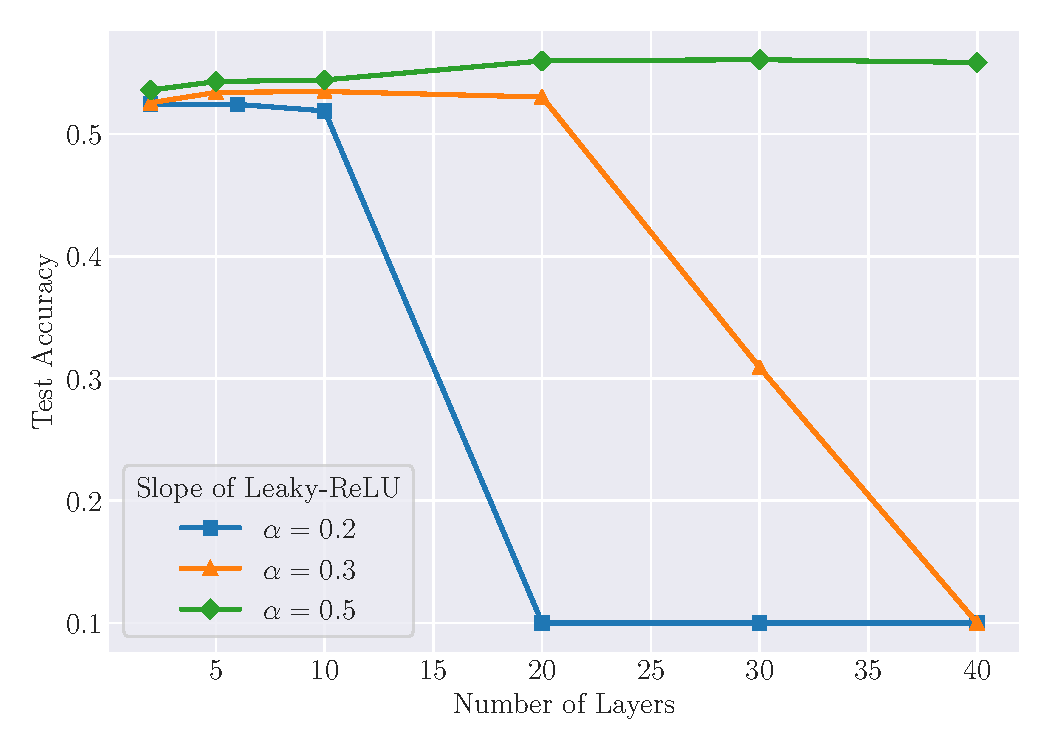
\includegraphics[width=\scalefigure\textwidth]{figures/main/ch4-diagonal_circulant/cifar10_leaky_relu.pdf}
  \caption{
    Impact of increasing the slope of a Leaky-ReLU in DCNNs.
    Deep DCNNs with a larger slope are easier to train.}
  \label{figure:ch4-cifar10_leaky_relu}
\end{figure}


We empirically found that the ReLU activations had an impact on the training of deep diagonal-circulant neural networks.
Indeed, the deeper the network, the more nonlinear it is, which makes convergence difficult.
In an experiment, we replace the ReLU activations with Leaky-ReLU activations (\cf \Cref{subsection:ch2-preliminaries_on_neural_networks}) and vary the slope of the Leaky-ReLU (a higher slope means an activation function that is closer to a linear function).
The results of this experiment are presented in~\Cref{figure:ch4-cifar10_leaky_relu}.

% In \Cref{figure:ch4-cifar10_leaky_relu}, we observe that reducing the nonlinearity of the networks can be used to train deeper networks.
In the experiment, we try different slopes for the Leaky-ReLU activation and train diagonal-circulant neural networks with different depth.
We can observe that a higher slope (making the network more linear) facilitates convergence, allowing us to train deeper networks.
This is an interesting result, since  we can use this technique to adjust the number of parameters in the network (increasing depth), without facing training difficulties.
We hence rely on this setting in the experimental section. 

\pagebreak

% Indeed, the more nonlinear activation a network 
%
% reducing the number of nonlinearities in the networks simplifies the training of deep neural networks.
%
% To support this claim, we conduct a series of experiments on various DCNNs with a varying number of ReLU activations (to reduce the number of nonlinearities, we replace some ReLU activations with the identity function).
%
% In a second experiment, 
%
% \todotext{update here}
% Replacing the ReLU activation by the identity function is equivalent to varying the number of factor in a layer.
% In \Cref{figure:ch4-cifar10_factor}, we compare diagonal-circulant neural networks with several values of $k$ which set the number of factors inside a layer as follows:
% \begin{equation}
%   \rho \left( \prod_{i=1}^{k} \Dmat^{(i)}\Cmat^{(i)} \xvec + \bvec \right)
% \end{equation}
% % ``ReLU(DC)'' means that we interleave ReLU activation functions between every diagonal-circulant matrix, whereas ReLU(DCDC) means we interleave a ReLU activation every other block etc.
% In both \Cref{figure:ch4-cifar10_factor,figure:ch4-cifar10_leaky_relu}, we observe that reducing the nonlinearity of the networks can be used to train deeper networks.
% This is an interesting result, since  we can use this technique to adjust the number of parameters in the network, without facing training difficulties.
% We obtain a maximum accuracy of 0.56 with one ReLU every three layers and leaky-ReLUs with a slope of 0.5.
% We hence rely on this setting in the experimental section. 
%
% \begin{figure}[htb]
%    \centering
%    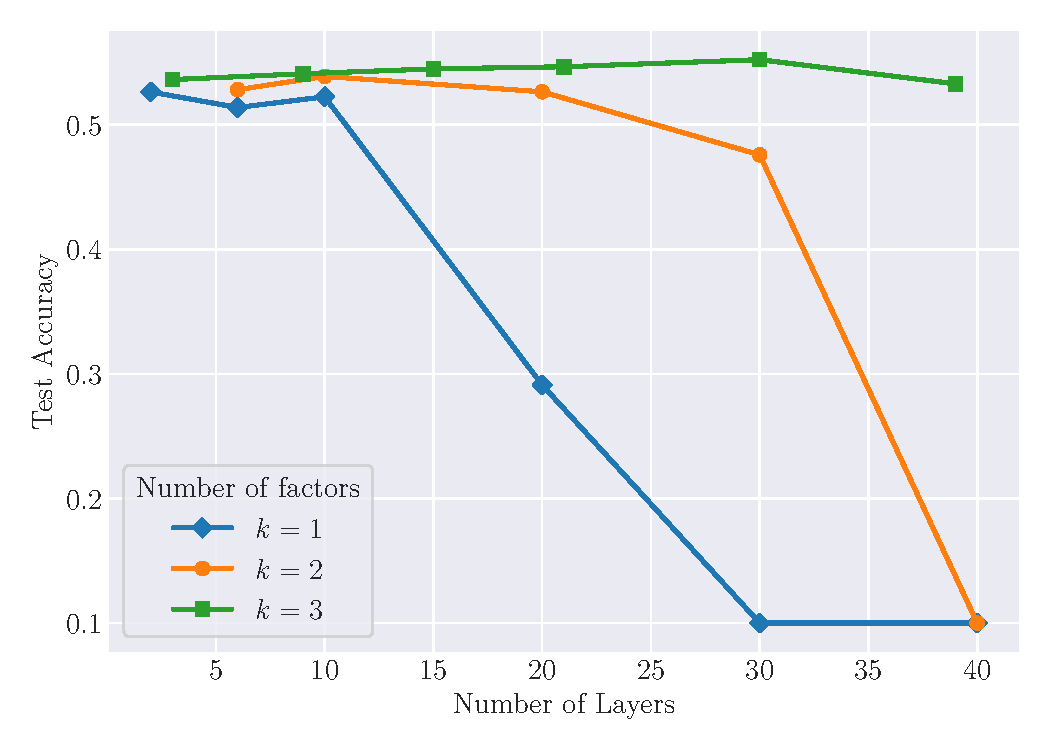
\includegraphics[width=\scalefigure\textwidth]{figures/main/ch4-diagonal_circulant/cifar10_factor.pdf}
%    \caption{
%       Impact of increasing the number of ReLU activations in a DCNN.
%       Deep DCNNs with fewer ReLUs are easier to train.}
%    \label{figure:ch4-cifar10_factor}
% \end{figure}


% \begin{figure}[ht]
%    \centering
%    \begin{subfigure}[b]{\textwidth}
%      \centering
%      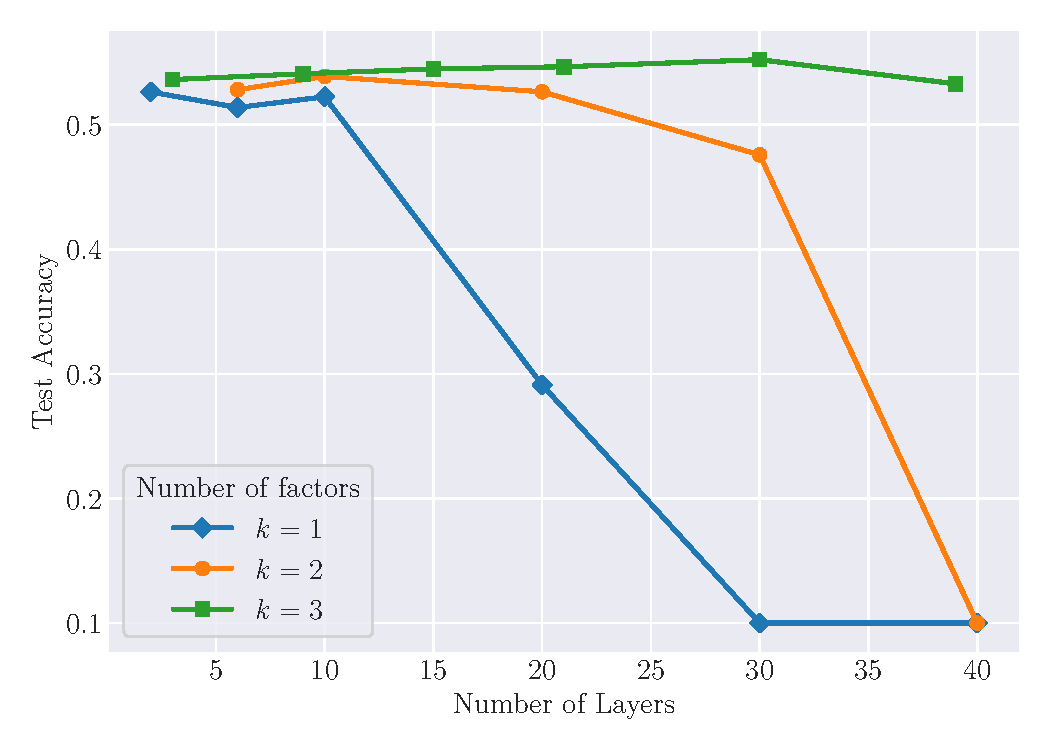
\includegraphics[width=\scalefigure\textwidth]{figures/main/ch4-diagonal_circulant/cifar10_factor.pdf}
%      \caption{
% 	Impact of increasing the number of ReLU activations in a DCNN.
% 	Deep DCNNs with fewer ReLUs are easier to train.}
%      \label{figure:ch4-cifar10_factor}
%    \end{subfigure}
%    \\[2cm]
%    \begin{subfigure}[b]{\textwidth}
%       \centering
%       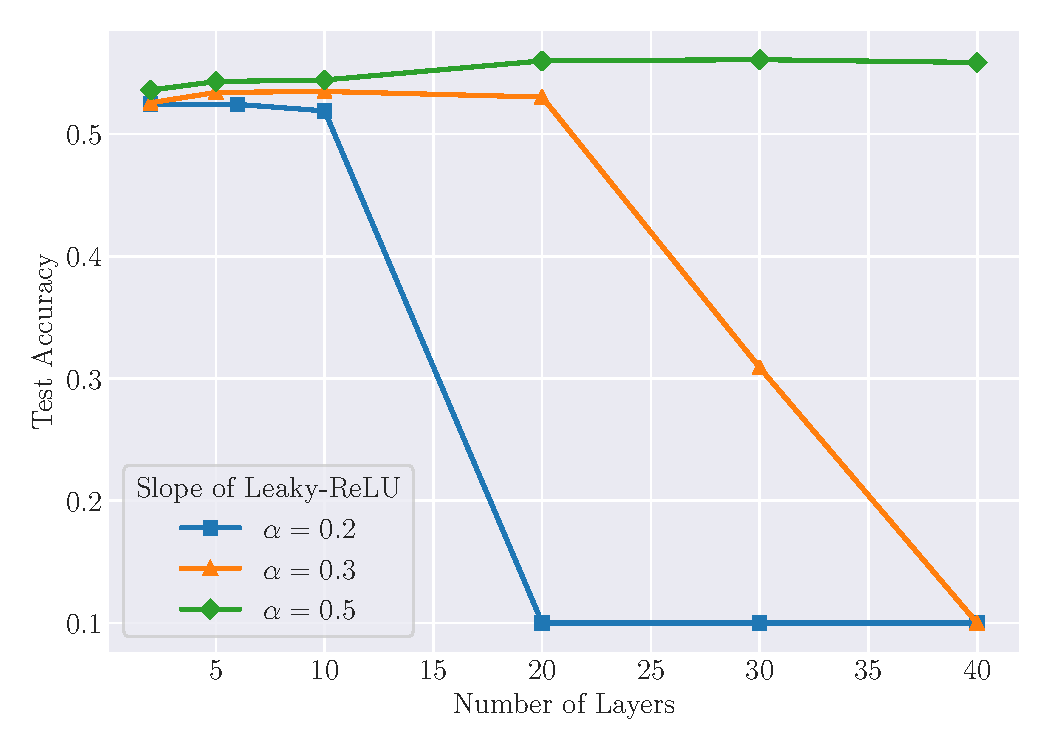
\includegraphics[width=\scalefigure\textwidth]{figures/main/ch4-diagonal_circulant/cifar10_leaky_relu.pdf}
%       \caption{
% 	Impact of increasing the slope of a Leaky-ReLU in DCNNs.
% 	Deep DCNNs with a larger slope are easier to train.}
%       \label{figure:ch4-cifar10_leaky_relu}
%    \end{subfigure}
%    \caption{xxx}
% \end{figure}



%%%%%%%%%%%%%%%%%%%%%%%%%%%%%%%%%%%%%%%%%%%%%%%%%%%%%%%%%%%%%%%%%%%%%%%%%%%%%%%
\section{Experiments}
\label{section:ch4-experiments}
%%%%%%%%%%%%%%%%%%%%%%%%%%%%%%%%%%%%%%%%%%%%%%%%%%%%%%%%%%%%%%%%%%%%%%%%%%%%%%%

This experimental section aims at answering the following questions:
\begin{enumerate}
    \itshape
    \item How do DCNNs compare to other approaches such as ACDC, LDR or other structured approaches?
    \item How do DCNNs compare to other compression based techniques?
    \item How do DCNNs perform in the context of large scale real-world machine learning applications?  
\end{enumerate}


%%%%%%%%%%%%%%%%%%%%%%%%%%%%%%%%%%%%%%%%%%%%%%%%%%%%%%%%%%%%%%%%%%%%%%%%%%%%%%%
\subsection{Comparison with other structured approaches}
\label{subsection:ch4-comparison_with_other_structured_approches}
%%%%%%%%%%%%%%%%%%%%%%%%%%%%%%%%%%%%%%%%%%%%%%%%%%%%%%%%%%%%%%%%%%%%%%%%%%%%%%%


% \begin{figure}
%    \centering
%    \begin{subfigure}[b]{0.75\textwidth}
%        \centering
%        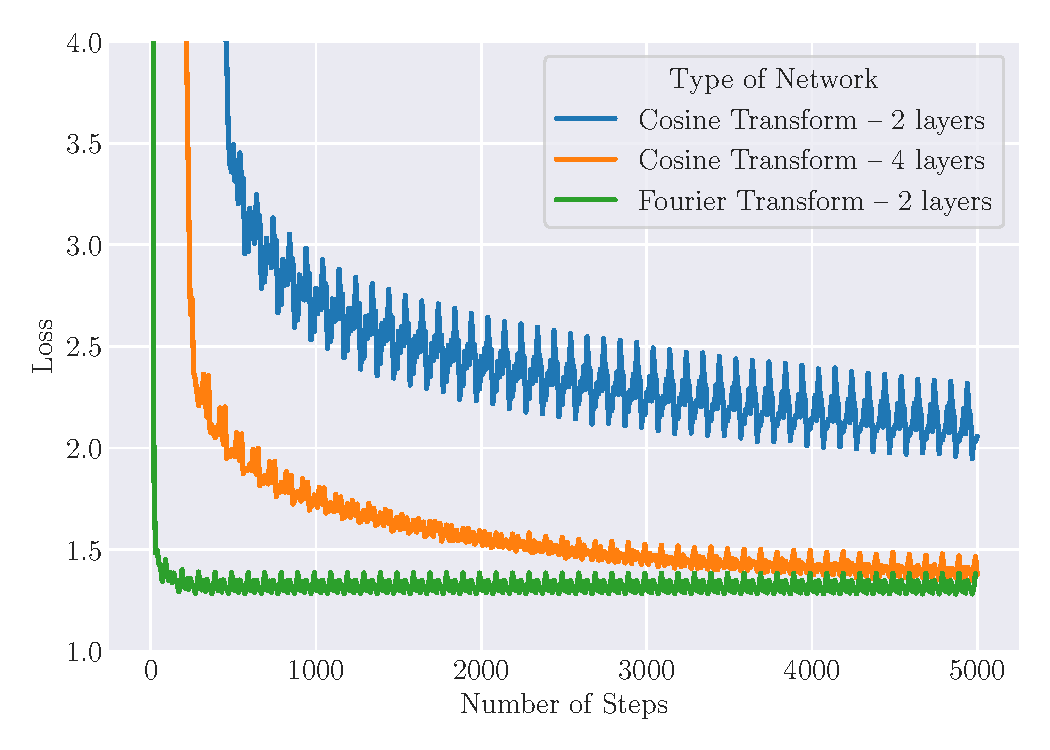
\includegraphics[width=\textwidth]{figures/main/ch4-diagonal_circulant/acdc_regression.pdf}
%        \caption{Evolution of the training loss on a regression task with synthetic data.}
%        \label{figure:ch4-acdc_regression}
%    \end{subfigure}
%    \\[2cm]
%    \begin{subfigure}[b]{0.75\textwidth}
%        \centering
%        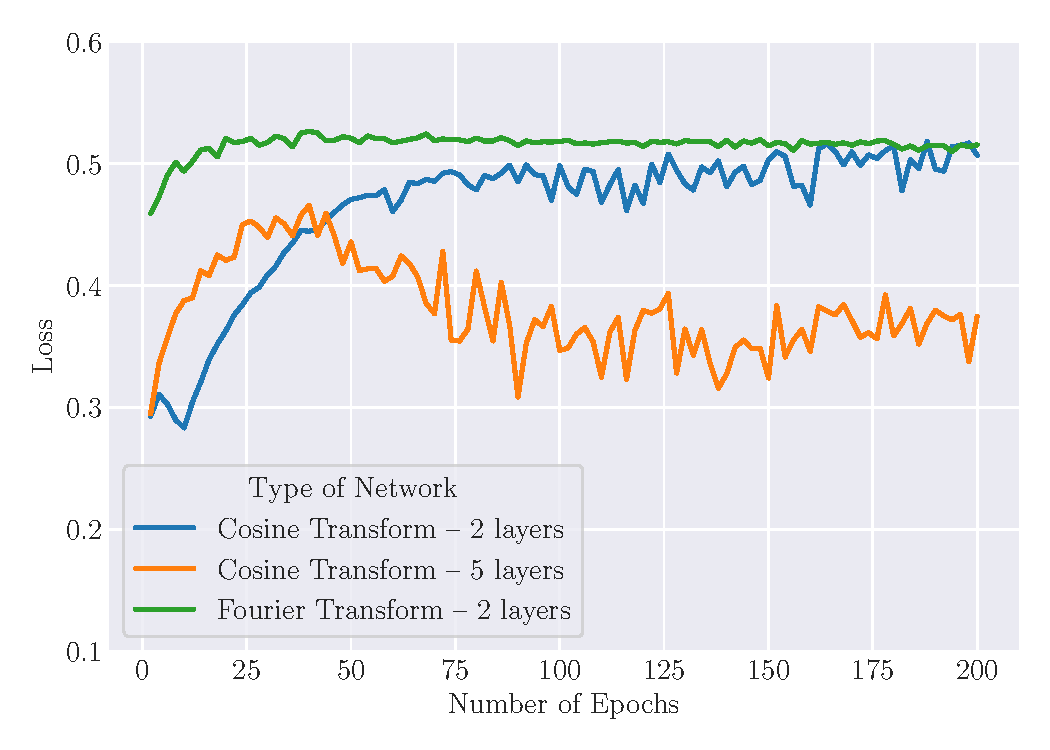
\includegraphics[width=\textwidth]{figures/main/ch4-diagonal_circulant/acdc_cifar10.pdf}
%        \caption{Test accuracy on the CIFAR-10 dataset.~\\ \phantom{.}}
%        \label{figure:ch4-acdc_cifar10}
%    \end{subfigure}
%    \caption{Comparison of DCNNs and \ACDC networks on two different tasks.}
% \end{figure}


\begin{figure}[ht]
   \centering
   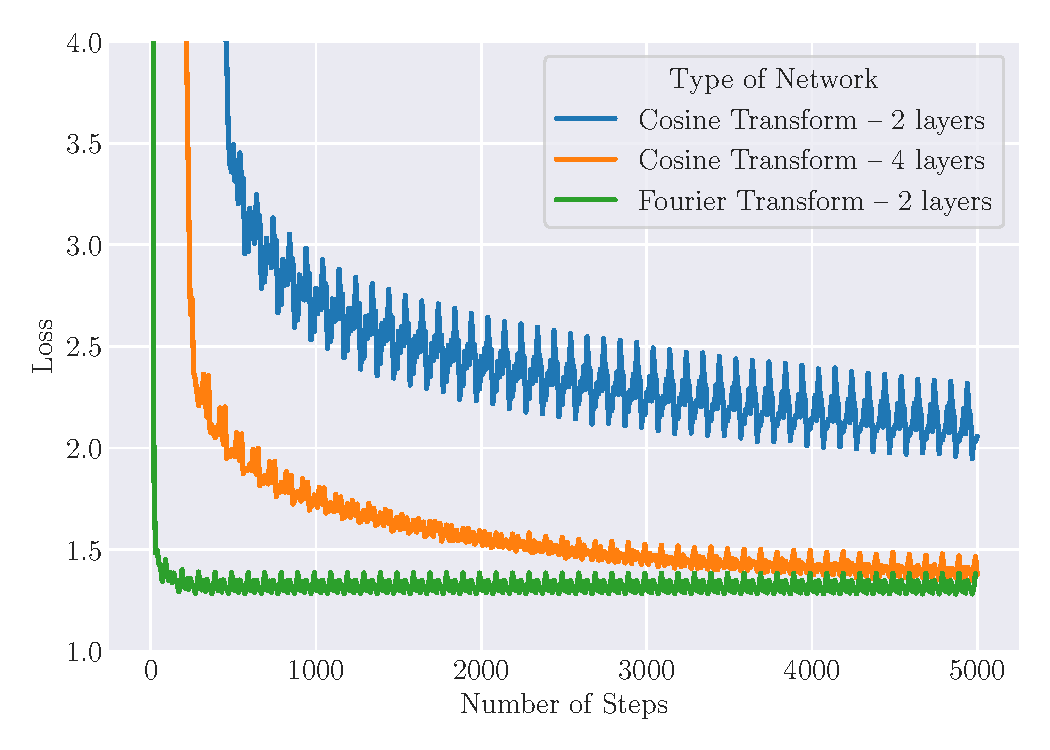
\includegraphics[width=\scalefigure\textwidth]{figures/main/ch4-diagonal_circulant/acdc_regression.pdf}
   \caption{Evolution of the training loss on a regression task with synthetic data.}
   \label{figure:ch4-acdc_regression}
\end{figure}

\begin{figure}[ht]
   \centering
   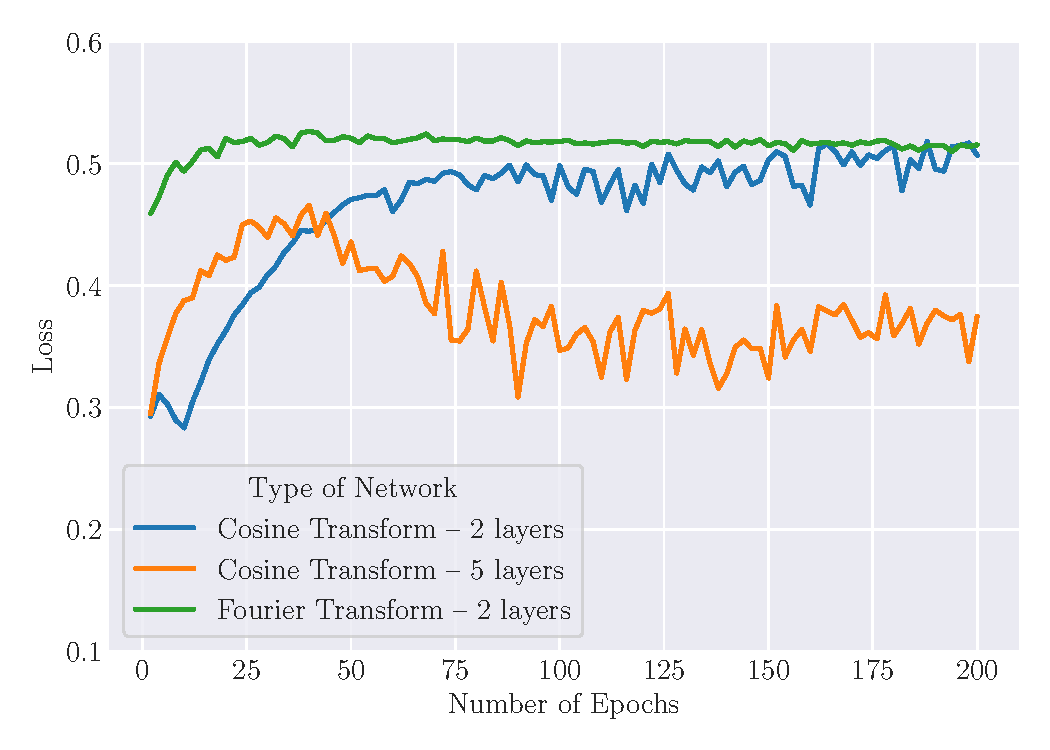
\includegraphics[width=\scalefigure\textwidth]{figures/main/ch4-diagonal_circulant/acdc_cifar10.pdf}
   \caption{Comparison of DCNNs and \ACDC networks on two different tasks. - Test accuracy on the CIFAR-10 dataset.}
   \label{figure:ch4-acdc_cifar10}
\end{figure}



%%%%%%%%%%%%%%%%%%%%%%%%%%%%%%%%%%%%%%%%%%%%%%%%%%%%%%%%%%%%%%%%%%%%%%%%%%%%%%%
\subsubsection{Comparison with \ACDC}
%%%%%%%%%%%%%%%%%%%%%%%%%%%%%%%%%%%%%%%%%%%%%%%%%%%%%%%%%%%%%%%%%%%%%%%%%%%%%%%

In \Cref{chapter:ch3-related_work}, we have discussed the differences between the \ACDC framework and our approach from a theoretical perspective.
In this section, we conduct experiments to compare the performance of DCNNs with neural networks based on \ACDC layers. 
We first reproduce the experimental setting from \citet{moczulski2016acdc}, and compare both approaches using only linear networks (\ie networks without any ReLU activations).
The synthetic dataset has been created in order to reproduce the experiment on the regression linear problem proposed by~\citet{moczulski2016acdc}.
We draw $\Xmat$ and $\Wmat$ from a uniform distribution between [-1, +1] and $\epsilon$ from a normal distribution with mean 0 and variance $0.01$.
The relationship between $\Xmat$ and $\Ymat$ is defined by $\Ymat = \Xmat\Wmat + \epsilon$. 
The results are presented in \Cref{figure:ch4-acdc_regression}.
In this simple setting, while both architectures demonstrate good performance, we can observe that DCNNs offer a better convergence rate.
In \Cref{figure:ch4-acdc_cifar10}, we compare neural networks with ReLU activations on CIFAR-10. 

We found that networks which are based only on \ACDC layers are difficult to train and offer poor accuracy on CIFAR-10 (we have tried different initialization schemes including the one from the original paper, and the one we introduce in this chapter).
\citet{moczulski2016acdc} manage to train a large VGG network  however these networks are generally highly redundant and the contribution of the structured layer is difficult to quantify. 
We also observe that adding a single dense layer improves the convergence rate of \ACDC in the linear case, which explains the good results of \citet{moczulski2016acdc}.
However, it is difficult to characterize the true contribution of the \ACDC layers when the network has a large number of expressive layers.

In contrast, deep DCNNs can be trained and offer good performance without additional dense layers (these results are in line with our experiments on the \yt dataset).
We can conclude that DCNNs are able to model complex relations at a low cost. 

% \begin{figure}
%    \centering
%    \begin{tikzpicture}[scale=0.8]
\begin{axis}[
    legend cell align={left},
    xlabel={\large \#weights (x1000) },
    ylabel={Test Accuracy},
    xmin=21, xmax=370,
    ymin=0.2, ymax=0.6,
    legend pos=south east,
    ymajorgrids=true,
    grid style=dashed,
	]
    \addplot[color=red, line width=0.25mm, dashed] table [y=accuracy, x=weights]
    {figures/main/ch4-diagonal_circulant/data/cifar10/type/dense.dat};
    \addplot[mark=triangle, color=blue, line width=0.4mm] table [y=accuracy, x=weights]
    {figures/main/ch4-diagonal_circulant/data/cifar10/type/circulant.dat};
    \addplot[mark=square, color=red, line width=0.4mm] table [y=accuracy, x=weights]
    {figures/main/ch4-diagonal_circulant/data/cifar10/type/diag_toeplitz.dat};
    \addplot[mark=o, color=gray, line width=0.4mm] table [y=accuracy, x=weights]
    {figures/main/ch4-diagonal_circulant/data/cifar10/type/toeplitz.dat};
    \addplot[mark=diamond, color=brown, line width=0.4mm] table [y=accuracy, x=weights]
    {figures/main/ch4-diagonal_circulant/data/cifar10/type/low_rank.dat};
    \legend{
      Dense (9M weights),
      DCNN,
      DTNN,
      Toeplitz network,
      Low Rank network, 
     }
\end{axis}
\end{tikzpicture}

%    \caption{Network size vs. Accuracy compared on Dense networks, DCNNs (our approach), DTNNs (our approach), neural networks based on Toeplitz matrices and neural networks based on Low Rank-based matrices. DCNNs outperforms alternatives structured approaches.}
%    \label{figure:ch4-cifar10_type}
% \end{figure}


\begin{figure}
   \centering
   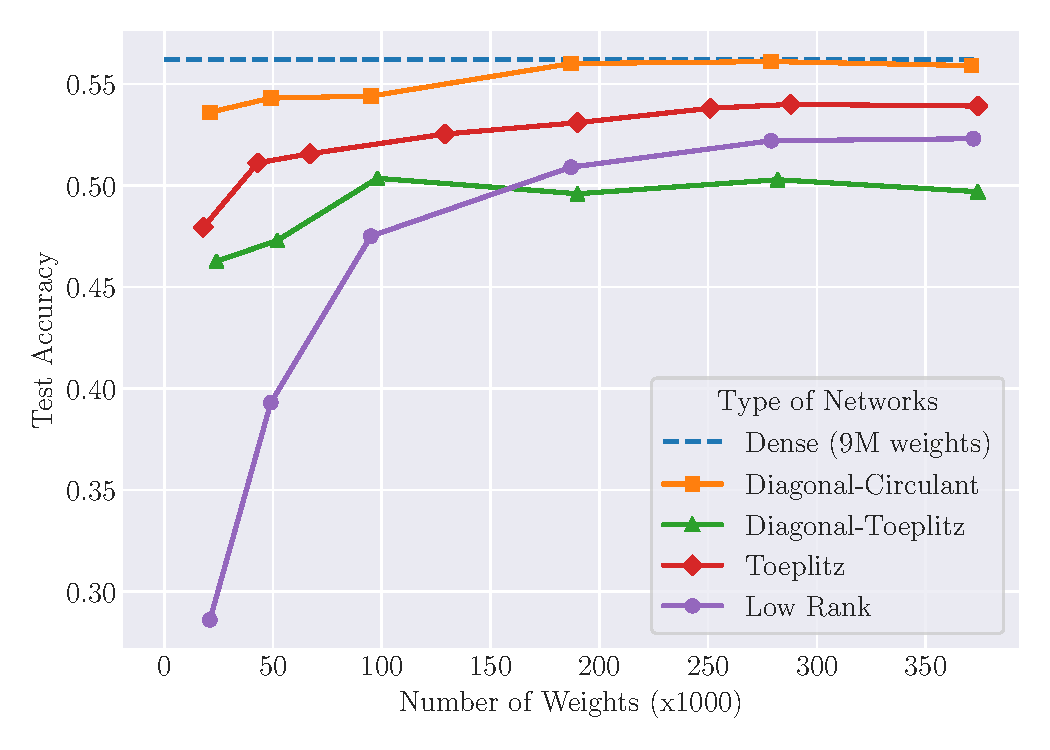
\includegraphics[width=\scalefigure\textwidth]{figures/main/ch4-diagonal_circulant/cifar10_type.pdf}
   \caption{Network size vs. Accuracy compared on Dense networks, DCNNs (our approach), DTNNs (our approach), neural networks based on Toeplitz matrices and neural networks based on Low Rank-based matrices. DCNNs outperforms alternatives structured approaches.}
   \label{figure:ch4-cifar10_type}
\end{figure}



\begin{figure}
   \centering
   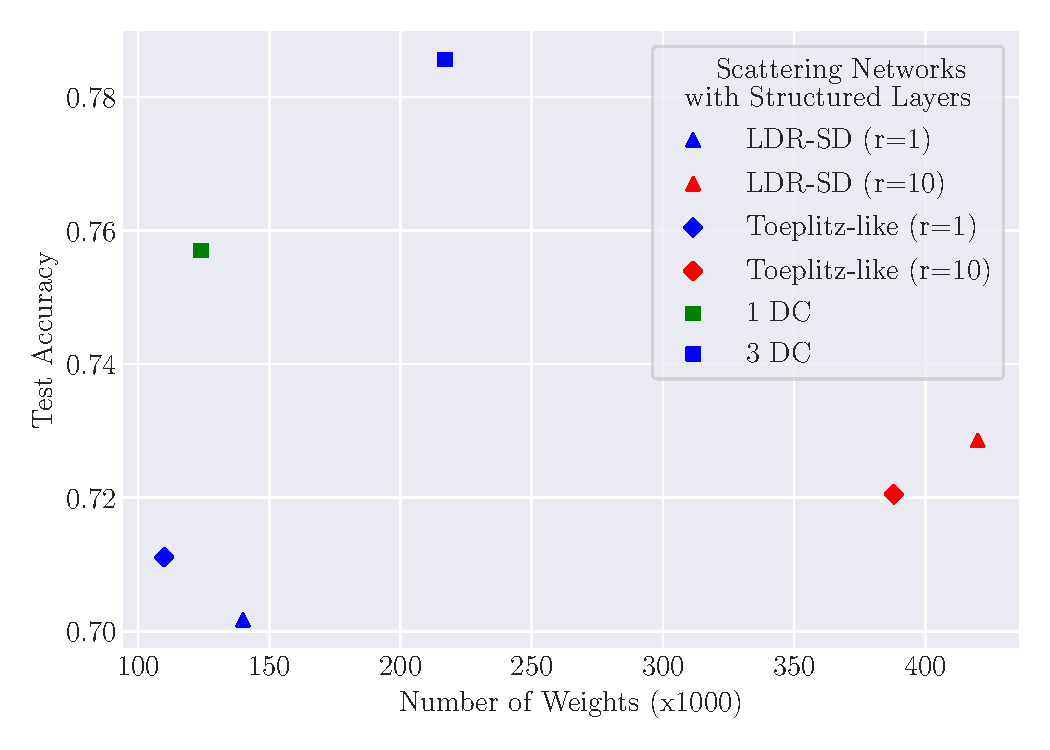
\includegraphics[width=\scalefigure\textwidth]{figures/main/ch4-diagonal_circulant/scatterplot.pdf}
   \caption{Accuracy of different structured architecture given the number of trainable parameters.}
   \label{figure:ch4-cifar10_with_channels_xp}
\end{figure}




%%%%%%%%%%%%%%%%%%%%%%%%%%%%%%%%%%%%%%%%%%%%%%%%%%%%%%%%%%%%%%%%%%%%%%%%%%%%%%%
\subsubsection{Comparison with Dense networks, Toeplitz networks and Low Rank networks.}
%%%%%%%%%%%%%%%%%%%%%%%%%%%%%%%%%%%%%%%%%%%%%%%%%%%%%%%%%%%%%%%%%%%%%%%%%%%%%%%

We now compare DCNNs with other state-of-the-art structured networks by measuring the accuracy on a flattened version of the CIFAR-10 dataset.
Our baseline is a dense feed-forward network with a fixed number of weights (9 million weights).
We compare with DCNNs and with DTNNs (see below), Toeplitz networks, and Low-Rank networks~\cite{yu2017compressing}.
We first consider Toeplitz networks which are stacked Toeplitz matrices interleaved with ReLU activations since Toeplitz matrices are closely related to circulant matrices.
However, Toeplitz networks have a different structure than DCNNs (they do not include diagonal matrices), therefore, we also experiment using DTNNs, a variant of DCNNs where all the circulant matrices have been replaced by Toeplitz matrices.
Finally we conduct experiments using networks based on low-rank matrices as they are also closely related to our work.
For each approach, we report the accuracy of several networks with a varying depth ranging from 1 to 40 (DCNNs, Toeplitz networks) and from 1 to 30 (from DTNNs).
For low-rank networks, we used a fixed depth network and increased the rank of each matrix from 7 to 40.
We also tried to increase the depth of low rank matrices, but we found that deep low-rank networks are difficult to train so we do not report the results here.
We compare all the networks based on the number of weights from 21K (0.2\% of the dense network) to 370K weights (4\% of the dense network) and we report the results in \Cref{figure:ch4-cifar10_type}. 
First we can see that the size of the networks correlates positively with their accuracy which demonstrated successful training in all cases.
We can also see that the DCNNs achieves the maximum accuracy of 56\% with 20 layers ($\sim$ 200K weights) which is as good as the dense networks with only 2\% of the number of weights.
Other approaches also offer good trade-offs but they are not able to reach the accuracy of a dense network.


%%%%%%%%%%%%%%%%%%%%%%%%%%%%%%%%%%%%%%%%%%%%%%%%%%%%%%%%%%%%%%%%%%%%%%%%%%%%%%%
\subsubsection{Comparison with LDR networks}
%%%%%%%%%%%%%%%%%%%%%%%%%%%%%%%%%%%%%%%%%%%%%%%%%%%%%%%%%%%%%%%%%%%%%%%%%%%%%%%

\begin{table}[htb]
  \centering
  \begin{tabular}{lcc}
    \toprule
    \textbf{Architectures} & \textbf{\#Parameters} & \textbf{Accuracy}  \\
    \midrule
    \textit{Dense} & \textit{9.4M}	 & \textit{0.562} \\
    \textbf{\textit{DCNN $(5\ layers)$}} & \textbf{49K}	& \textbf{0.543} \\
    \textbf{\textit{DCNN $(2\ layers)$}} & \textbf{21K} & \textbf{0.536} \\
    LDR--TD	$(r = 2)$	         & 64K	& 0.511 \\
    LDR--TD	$(r = 3)$	         & 70K	& 0.473 \\
    Toeplitz-like $(r=2)$	         & 46K	& 0.483 \\
    Toeplitz-like $(r =3)$	         & 52K  & 0.496 \\
    \bottomrule
    \end{tabular}
    \caption{LDR networks compared with DCNNs on a flattend version of CIFAR-10. DCNNs outperform all LDR configurations with fewer weights. Remark: the numbers may differ from the original experiments by~\citet{thomas2018learning} because we use the original dataset instead of a monochrome version.}
    \label{table:ch4-xp_ldr}
\end{table}

We now compare DCNNs with the LDR framework using the network configuration experimented in the original paper \cite{thomas2018learning}: a single LDR structured layer followed by a dense layer.
In the LDR framework, we can change the size of a network by adjusting the rank of the residual matrix, effectively capturing matrices with a structure that is close to a known structure but not exactly (in the LDR framework, Toeplitz matrices can be encoded with a residual matrix with rank=2, so a matrix that can be encoded with a residual of rank=3 can be seen as Toeplitz-like.).
The results are presented in \Cref{table:ch4-xp_ldr} and demonstrate that DCNNs outperforms all LDR networks both in terms in size and accuracy.


%%%%%%%%%%%%%%%%%%%%%%%%%%%%%%%%%%%%%%%%%%%%%%%%%%%%%%%%%%%%%%%%%%%%%%%%%%%%%%%
\subsection{Comparison with other compression based approaches}
\label{subsection:ch4-comparison_with_other_compression_based_approaches}
%%%%%%%%%%%%%%%%%%%%%%%%%%%%%%%%%%%%%%%%%%%%%%%%%%%%%%%%%%%%%%%%%%%%%%%%%%%%%%%


\begin{table}
  \centering
    \caption{Comparison with compression based approaches}
    \begin{tabular}{lcrc}
    \toprule
    \multicolumn{1}{c}{\textbf{Architecture}} & \multicolumn{1}{c}{\textbf{\#Params}} & \textbf{Error (\%)} \\
    \hline \\
    \textit{LeNet \cite{Lecun98gradient-basedlearning}} & \textit{4 257 674} & \textit{0.61} \\
    \multirow{2}[0]{*}{\textbf{DCNN}} & \textbf{25 620} & \textbf{1.74} \\
          & \textbf{31 764} & \textbf{1.60} \\
    \multirow{2}[0]{*}{HashNet \cite{chen2015compressing}} & 46 875 & 2.79 \\
          &  78 125 & 1.99 \\
    \multirow{2}[0]{*}{Dark Knowledge \cite{hinton2015distilling}} & 46 875 & 6.32 \\
          &  78 125 & 2.16 \\
    \bottomrule
    \end{tabular}%
  \label{tab:mnist}%
\end{table}%


We provide a comparison with other compression based approaches such as HashNet \cite{chen2015compressing}, Dark Knowledge \cite{hinton2015distilling} and Fast Food Transform (FF) \cite{yang2015deep}. 
\Cref{tab:mnist} shows the test error of DCNN against other known compression techniques on the MNIST datasets.
We can observe that DCNN outperforms HashNet \cite{chen2015compressing} and Dark Knowledge \cite{hinton2015distilling} with fewer number of parameters.
The architecture with Fast Food (FF) \cite{yang2015deep} achieves better performance but with convolutional layers and only $1$ Fast Food Layer as the last Softmax layer. 

%%%%%%%%%%%%%%%%%%%%%%%%%%%%%%%%%%%%%%%%%%%%%%%%%%%%%%%%%%%%%%%%%%%%%%%%%%%%%%%
\subsection{Large-scale video classification on the \yt dataset}
\label{subsection:ch4-large_scale_video_classification}
%%%%%%%%%%%%%%%%%%%%%%%%%%%%%%%%%%%%%%%%%%%%%%%%%%%%%%%%%%%%%%%%%%%%%%%%%%%%%%%

To understand the performance of deep DCNNs on large scale applications, we conducted experiments on the \yt video classification with 3.8 training examples introduced by~\citet{abu2016youtube}.
Notice that we favour this experiment over ImageNet applications because modern image classification architectures involve a large number of convolutional layers, and compressing convolutional layers is out of our scope. 
Also, as mentioned earlier, testing the performance of DCNN architectures mixed with a large number of expressive layers makes little sense.
The \yt includes two datasets describing 8 million labeled videos.
Both datasets contain audio and video features for each video.
In the first dataset (\emph{aggregated}) all audio and video features have been aggregated every 300 frames.
The second dataset (\emph{full}) contains the descriptors for all the frames.
To compare the models we use the GAP metric (Global Average Precision) proposed by~\citet{abu2016youtube}.
On the simpler \emph{aggregated} dataset we compared off-the-shelf DCNNs with a dense baseline with 5.7M weights.
On the full dataset, we designed three new compact architectures based on the state-of-the-art architecture introduced by~\citet{abu2016youtube}. 

\paragraph{Experiments on the aggregated dataset with DCNNs}
We compared DCNNs with a dense baseline with 5.7 millions weights.
The goal of this experiment is to discover a good trade-off between depth and model accuracy.
To compare the models we use the GAP metric (Global Average Precision) following the experimental protocol in~\cite{abu2016youtube}, to compare our experiments. 

\Cref{table:youtube_agg_xp} shows the results of our experiments on the \emph{aggregated} \yt dataset in terms of number of weights, compression rate and GAP.
We can see that the compression ratio offered by the circulant architectures is high.
This comes at the cost of a little decrease of GAP measure.
The 32 layers DCNN is 46 times smaller than the original model in terms of number of parameters while having a close performance. 


\begin{table}
  \centering
  \caption{This table shows the GAP score for the \yt dataset with DCNNs. We can see a large increase in the score with deeper networks.}
  \begin{tabular}{lccc}
    \toprule
    \textbf{Architecture} & \textbf{\#Weights} &
    \textbf{GAP@20} \\
    \hline \\
    \textit{original} & \textit{5.7M} & \textit{0.773} \\
    4 DC & 25 410  (\textit{\textbf{0.44}}) & 0.599   \\
    32 DC  & 122 178 \textit{(2.11)} & 0.685   \\
    4 DC + 1 FC & 4.46M \textit{(77)} & \textbf{0.747} \\
  \hline
  \end{tabular}
  \label{table:youtube_agg_xp}
\end{table}

\begin{table}
  \centering
  \caption{This table shows the GAP score for the \yt dataset with different layer represented with our DC decomposition.}
  \begin{tabular}{lccc}
  \toprule
  \textbf{Architecture} & \textbf{\#Weights} & \textbf{GAP@20} \\
  \hline \\
  \textit{original} & \textit{45M} & \textit{0.846} \\
  DBoF with DC   & 36M (\textit{80}) & 0.838 \\
  FC with DC    & 41M (\textit{91}) & \textbf{0.845} \\
  MoE with DC   & 12M (\textit{\textbf{26}}) & 0.805 \\
  \hline
  \end{tabular}
  \label{table:youtube_full_xp}
\end{table}

\paragraph{Experiments with DCNNs Deep Bag-of-Frames Architecture:}
The Deep Bag-of-Frames architecture can be decomposed into three blocks of layers, as illustrated in \Cref{figure:ch4-archi_youtube}.
The first block of layers, composed of the Deep Bag-of-Frames embedding (DBoF), is meant to model an embedding of these frames in order to make a simple representation of each video.
A second block of fully connected layers (FC) reduces the dimensionality of the output of the embedding and merges the resulting output with a concatenation operation.
Finally, the classification block uses a combination of Mixtures-of-Experts (MoE)~\cite{jordan1993hierarchical,abu2016youtube} and Context Gating~\cite{miech2017learnable} to calculate the final class probabilities.
\Cref{table:youtube_full_xp} shows the results in terms of number of weights, size of the model (MB) and GAP on the full dataset, replacing the DBoF block reduces the size of the network without impacting the accuracy.
We obtain the best compression ratio by replacing the MoE block with DCNNs (26\%) of the size of the original dataset with a GAP score of 0.805 (95\% of the score obtained with the original architecture).
We conclude that DCNN are both theoretically sound and of practical interest in real, large scale applications.

\begin{figure}[htb]
  \centering
  \tikzset{%
  >={Latex[width=2mm,length=2mm]},
  % Specifications for style of nodes:
            base/.style = {rectangle, draw=black, text centered, font=\sffamily},
             box/.style = {base, rounded corners, text depth=3cm, minimum height=4cm, minimum width=3cm},
     transparent/.style = {rectangle, draw=black},
       circulant/.style = {base, fill=yellow!30},
       embedding/.style = {base, fill=blue!30, minimum width=2.5cm, minimum height=1cm},
           other/.style = {base, fill=white!30,  minimum width=2cm, minimum height=1cm},
              fc/.style = {base, fill=orange!30, minimum width=1.5cm, minimum height=1cm},
          gating/.style = {base, fill=green!30, minimum width=2cm, text width=2cm, minimum height=1cm},
             moe/.style = {base, fill=purple!30, minimum width=1.5cm, minimum height=1cm},
}

\begin{tikzpicture}[every node/.style={fill=white, font=\sffamily}, align=center]

  \draw (0.0, +2.)  node [other, draw=none] {\textbf{Embedding}};
  \draw (+3.7, +2.)  node [other, draw=none] {\textbf{Dim Reduction}};
  \draw (+8.0, +2.)  node [other, draw=none] {\textbf{Classification}};

  \draw (0, +0.8)  node [embedding] {Video};
  \draw (0, -0.8)  node [embedding] {Audio};

  \draw (+2.5, +0.8)  node (fc) [fc] {FC};
  \draw (+2.5, -0.8)  node (fc) [fc] {FC};

  \draw (+4.75, 0)  node (fc) [other] {concat};
  \draw (+7.0, 0)  node (moe) [moe] {MoE};
  \draw (+9.25, 0)  node (gating2) [gating] {Context Gating};
 
  \draw (+1.5, +2) [dashed] -- (+1.5, -1.7);
  \draw (+6, +2) [dashed] -- (+6, -1.7);
  
\end{tikzpicture}

  \caption{This figure shows the state-of-the-art neural network architecture, initially proposed by~\citet{abu2016youtube} and later improved by~\citet{miech2017learnable}, used in our experiment.}
  \label{figure:ch4-archi_youtube}
\end{figure}

\paragraph{Architectures \& Hyper-Parameters:} 
For the first set of our experiments (\emph{experiments on CIFAR-10}), we train all networks for 200 epochs, a batch size of 200, Leaky ReLU activation with a different slope.
We minimize the Cross Entropy Loss with Adam optimizer and use a piecewise constant learning rate of $5 \times 10^{-5}$, $2.5\times10^{-5}$, $5\times10^{-6}$ and $1\times10^{-6}$ after respectively 40K, 60K and 80K steps.
For the \yt dataset experiments, we built a neural network based on state-of-the-art architecture initially proposed by~\citet{abu2016youtube} and later improved by~\citet{miech2017learnable}.
Remark that no convolution layer is involved in this application since the input vectors are embeddings of video frames processed using state-of-the-art convolutional neural networks trained on ImageNet.
We trained our models with the CrossEntropy loss and used Adam optimizer with a 0.0002 learning rate and a 0.8 exponential decay every 4 million examples.
All fully connected layers are composed of 512 units.
DBoF, NetVLAD and NetFV are respectively 8192, 64 and 64 of cluster size for video frames and 4096, 32, 32 for audio frames.
We used 4 mixtures for the MoE Layer.
We used all the available 300 frames for the DBoF embedding.
In order to stabilize and accelerate the training, we used batch normalization before each non linear activation and gradient clipping. 


%%%%%%%%%%%%%%%%%%%%%%%%%%%%%%%%%%%%%%%%%%%%%%%%%%%%%%%%%%%%%%%%%%%%%%%%%%%%%%%
\subsection{Exploiting Image Features}
%%%%%%%%%%%%%%%%%%%%%%%%%%%%%%%%%%%%%%%%%%%%%%%%%%%%%%%%%%%%%%%%%%%%%%%%%%%%%%%

\begin{table}[htb]
  \centering
  \begin{tabular}{lcc}
    \toprule
    \textbf{Architectures} & \textbf{\#Parameters} & \textbf{Accuracy}  \\
    \midrule
    \textbf{DC $(1\ layers)$} & \textbf{124K} & \textbf{0.757} \\
    \textbf{DC $(3\ layers)$} & \textbf{217K} & \textbf{0.785} \\
    % \textbf{Ensemble x5 DC $(3\ layers)$} &  \textbf{1.08M} & \textbf{0.811} \\
    LDR-SD $(r=1)$ & 140K & 0.701 \\
    LDR-SD $(r=10)$ & 420K & 0.728 \\
    Toeplitz-like $(r=1)$ & 110K & 0.711 \\
    Toeplitz-like $(r=10)$ & 388K & 0.720 \\
    \bottomrule
    \end{tabular}
    \caption{Two depths scattering on CIFAR-10 followed by LDR or DC layer. Networks with DC layers outperform all LDR configurations with fewer weights.}
    \label{table:ch4-xp_ldr_scattering}
\end{table}




Dense layers and DCNNs are not designed to capture task-specific features such as the translation invariance inherently useful in image classification.
We can further improve the accuracy of such general purpose architectures on image classification without dramatically increasing the number of trained parameters by stacking them on top of fixed (ie non-trained) transforms such as the scattering transform \cite{mallat2010recursive}.
In this section we compare the accuracy of various structured networks, enhanced with the scattering transform, on an image classification task, and run comparative experiments on CIFAR-10. 

Our test architecture consists of 2 depth scattering on the RGB images followed by a batch norm and LDR or DC layer.
To vary the number of parameters of Scattering+LDR architecture, we increase the rank of the matrix (stacking several LDR matrices quickly exhausted the memory).
The \Cref{figure:ch4-cifar10_with_channels_xp} and \Cref{table:ch4-xp_ldr_scattering} shows the accuracy of these architectures given the number of trainable parameters.

First, we can see that the DCNN architecture very much benefits from the scattering transform and is able to reach a competitive accuracy over 78\%.
We can also see that scattering followed by a DC layer systematically outperforms scattering + LDR or scattering + Toeplitz-like with less parameters. 





%%%%%%%%%%%%%%%%%%%%%%%%%%%%%%%%%%%%%%%%%%%%%%%%%%%%%%%%%%%%%%%%%%%%%%%%%%%%%%%
\section{Conclusion}
\label{section:ch4-discussion}
%%%%%%%%%%%%%%%%%%%%%%%%%%%%%%%%%%%%%%%%%%%%%%%%%%%%%%%%%%%%%%%%%%%%%%%%%%%%%%%

% \todotext{review this conclusion}
% \todotext{we need to open on the next chapter}

This chapter deals with the training of diagonal circulant neural networks.
To the best of our knowledge, training such networks with a large number of layers had not been done before.
We also endowed this kind of models with theoretical guarantees, hence enriching and refining previous theoretical work from the literature.
More importantly, we showed that DCNNs outperform their competing structured alternatives, including the very recent general approach based on LDR networks.
Our results suggest that stacking diagonal circulant layers with non linearities improves the convergence rate and the final accuracy of the network.
Formally proving these statements constitutes the future directions of this work.
We would like to generalize the good results of DCNNs to convolutional neural networks.
We also believe that circulant matrices deserve a particular attention in deep learning because of their strong ties with convolutions: a circulant matrix operator is equivalent to the convolution operator with circular paddings.
This fact makes any contribution to the area of circulant matrices particularly relevant to the field of deep learning with impacts beyond the problem of designing compact models.
As future work, we would like to generalize our results to deep convolutional neural networks. 


  %%%%%%%%%%%%%%%%%%%%%%%%%%%%%%%%%%%%%%%%%%%%%%%%%%%%%%%%%%%%%%%%%%%%%%%%%%%%%%%
\chapter{Bound on the Lipschitz Constant of Convolution Layers}
\label{chapter:ch5-lipschitz_bound}
%%%%%%%%%%%%%%%%%%%%%%%%%%%%%%%%%%%%%%%%%%%%%%%%%%%%%%%%%%%%%%%%%%%%%%%%%%%%%%%
\localtoc


%%%%%%%%%%%%%%%%%%%%%%%%%%%%%%%%%%%%%%%%%%%%%%%%%%%%%%%%%%%%%%%%%%%%%%%%%%%%%%%
\section{Introduction}
\label{section:ch5-introduction}
%%%%%%%%%%%%%%%%%%%%%%%%%%%%%%%%%%%%%%%%%%%%%%%%%%%%%%%%%%%%%%%%%%%%%%%%%%%%%%%


% The last few years have witnessed a growing interest in Lipschitz regularization of neural networks, with the aim of improving their generalization~\cite{bartlett2017spectrally}, their robustness to adversarial attacks~\cite{tsuzuku2018lipschitz, farnia2018generalizable}, or their generation abilities (\eg for GANs: \citet{miyato2018spectral,arjovsky2017wasserstein}).
% Unfortunately computing  the exact Lipschitz constant of a neural network is NP-hard~\cite{scaman2018lipschitz} and in practice, existing techniques such as~\citet{scaman2018lipschitz}, \citet{fazlyab2019efficient} or~\citet{latorre2020lipschitz} are difficult to implement for neural networks with more than one or two layers, which hinders their use in deep learning applications.
%
% To overcome this difficulty, most of the work has focused on computing the Lipschitz constant of \emph{individual layers} instead.
% The product of the Lipschitz constant of each layer is an upper-bound for the Lipschitz constant of the entire network, and it can be used as a surrogate to perform Lipschitz regularization.
% Since most common activation functions (such as ReLU) have a Lipschitz constant equal to one, the main bottleneck is to compute the Lipschitz constant of the underlying linear application which is equal to its largest singular value.
% The work in this line of research mainly relies on the celebrated iterative algorithm by~\citet{golub2000eigenvalue} used to approximate the maximum singular value of a linear function.
% Although generic and accurate, this technique is also computationally expensive, which impedes its usage in large training settings.

In this chapter we introduce a new upper bound on the largest singular value of convolution layers that is both tight and easy to compute.
Instead of using the power method to iteratively approximate this value, we study the properties of \emph{doubly-block Toeplitz matrices} and its links with Fourier analysis. 
% on Toeplitz matrix theory and its links with Fourier analysis.
% In order to devise a bound on the Lipschitz constant of a convolution layer as used by the Deep Learning community, we study the properties of \emph{doubly-block Toeplitz matrices}. 
Our work is based on the result of~\citet{gray2006toeplitz} which states that an upper bound on the singular value of Toeplitz matrices can be computed from the inverse Fourier transform of the characteristic sequence of these matrices.
We first extend this result to doubly-block Toeplitz matrices (\ie, block Toeplitz matrices where each block is Toeplitz) and then to convolutional operators, which can be represented as stacked sequences of doubly-block Toeplitz matrices.
From our analysis immediately follows an algorithm for bounding the Lipschitz constant of a convolution layer, and by extension the Lipschitz constant of the whole network.
We theoretically study the approximation of this algorithm and show experimentally that it is more efficient and accurate than competing approaches.

Finally, we illustrate our approach on adversarial robustness.
Recent work has shown that empirical methods such as adversarial training (AT) offer poor generalization~\cite{schmidt2018adversarially}, and can be improved by applying Lipschitz regularization~\cite{farnia2018generalizable}.
To illustrate the benefit of our new method, we train a large Wide ResNet with Lipschitz regularization and show that it offers a significant improvement over adversarial training alone, and over other methods for Lipschitz regularization.
In summary, we make the three following contributions:
\begin{enumerate}
  \item We devise an upper bound on the singular values of the operator matrix of convolution layers by leveraging Toeplitz matrix theory and its links with Fourier analysis.
  \item We propose an efficient algorithm to compute this upper bound which enables its use in the context of Convolutional Neural Networks.
  \item We use our method to regularize the Lipschitz constant of neural networks for adversarial robustness and show that it offers a significant improvement over AT alone.
\end{enumerate}


%%%%%%%%%%%%%%%%%%%%%%%%%%%%%%%%%%%%%%%%%%%%%%%%%%%%%%%%%%%%%%%%%%%%%%%%%%%%%%%
\section{Results on the Spectrum of Matrices from the Toeplitz Family}
\label{section:ch5-results_on_the_spectrum_of_matrices_from_the_toeplitz_family}
%%%%%%%%%%%%%%%%%%%%%%%%%%%%%%%%%%%%%%%%%%%%%%%%%%%%%%%%%%%%%%%%%%%%%%%%%%%%%%%

%%%%%%%%%%%%%%%%%%%%%%%%%%%%%%%%%%%%%%%%%%%%%%%%%%%%%%%%%%%%%%%%%%%%%%%%%%%%%%%
\subsection{Upper-Bounds on the Largest Singular Value of Toeplitz and Block Toeplitz Matrices}
\label{subsection:ch5-upper_bounds_on_the_largest_singular_value_of_toeplitz_and_block_toeplitz_matrices}
%%%%%%%%%%%%%%%%%%%%%%%%%%%%%%%%%%%%%%%%%%%%%%%%%%%%%%%%%%%%%%%%%%%%%%%%%%%%%%%

Doubly-block Toeplitz matrices inherit the properties of Toeplitz and block Toeplitz matrices.
Recall that for Toeplitz and block Toeplitz matrices, there exist no closed-form expression to compute their eigenvalues.
However, we can represent Toeplitz and block Toeplitz matrices with a 2$\pi$-periodic function which can describe very precisely the spectrum of the matrices. 
% Let $\{a_h\}_{h \in \Iset_n}$ be the characteristic sequence of a Toeplitz matrix $\Amat = \leftmat a_{j-i} \rightmat_{i,j \in \Iset_n} \in \Rbb^{n \times n}$ and let $\{\Bmatsf^{(h)}\}_{h \in \Iset_n}$ be the characteristic sequence of $m \times m$ blocks of a block Toeplitz matrix $\Bmat = \leftmat \Bmatsf^{(j-i)} \rightmat_{i,j \in \Iset_n} \in \Rbb^{nm \times nm}$ with $\Iset_n = \left\{ -n+1, \cdots, n-1 \right\}$.
Let $\{a_h\}_{h \in \Iset_n}$ be the characteristic sequence of a Toeplitz matrix $\Amat \in \Rbb^{n \times n}$ and let $\{\Bmatsf^{(h)}\}_{h \in \Iset_n}$ be the characteristic sequence of $m \times m$ blocks of a block Toeplitz matrix $\Bmat = \in \Rbb^{nm \times nm}$ such that $\Amat = (a_{j-i})_{i,j\in \Iset_n}$ and $\Bmat = (\Bmatsf^{(j-i)})_{i,j \in \Iset_n}$ with $\Iset_n = \left\{ -n+1, \cdots, n-1 \right\}$.
% The matrices are therefore denoted $\Amat = \leftmat a_{j-i} \rightmat_{i,j \in \Iset_n}$ and $\Bmat = ( \Bmatsf^{(j-i)} )_{i,j \in \Iset_n}$ 
Building on the results presented in the Background (\Cref{chapter:ch2-background}), we can define two trigonometric polynomials $f: \Rbb \rightarrow \Cbb$ and $F: \Rbb \rightarrow \Cbb^{m \times m}$ as follows:
\begin{equation}
  f(\omega) \triangleq \sum_{h \in \Iset_n} a_h e^{\ci h \omega} \quad \quad F(\omega) \triangleq \sum_{h \in \Iset_n} \Bmatsf^{(h)} e^{\ci h \omega} \enspace.
\end{equation}
$f(\omega)$  and $F(\omega)$ are the \emph{inverse Fourier transforms} of the sequences $\{a_h\}_{h \in \Iset_n}$ and $\{\Bmatsf^{(h)}\}_{h \in \Iset_n}$ respectively.
From there, inspired by the work done by~\citet{grenander1958toeplitz}, we recall from \Cref{subsection:ch2-a_fourier_representation_of_toeplitz_matrices} the operator $\Tmat$ mapping integrable functions to Toeplitz matrices:
\begin{equation} \label{equation:expression_toeplitz_matrix}
  \Tmat_n(f) \triangleq\leftmat\frac{1}{2\pi} \int_{0}^{2\pi} e^{-\ci(i-j)\omega} f(\omega) \diff \omega \rightmat_{i,j \in \Iset^+_n} \enspace,
\end{equation}
with this operator, we have $\Tmat(f) = \Amat$ and $\Tmat(F) = \Bmat$.

Now, we can state two known theorems which upper bound the largest singular value of Toeplitz and block Toeplitz matrices with respect to their generating functions.
\begin{theorem}[Bound on the singular values of Toeplitz matrices] \label{theorem:teoplitz_sup_singular}
  Let $f: \Rbb \rightarrow \Cbb$, be a continuous and $2\pi$-periodic function, then $\Tmat(f) \in \Rbb^{n \times n}$ is a Toeplitz matrix generated by the function $f$
  We can bound the largest singular value of the Toeplitz matrix $\Tmat(f)$ as follows:
  \begin{align}
    \sigma_1 \left( \Tmat(f) \right) \leq \sup_{\omega \in [0, 2\pi]} |f(\omega)|.
  \end{align}
  \removespace
\end{theorem}
\noindent
\Cref{theorem:teoplitz_sup_singular} is a direct application of Lemma 4.1 in~\citet{gray2006toeplitz} for real Toeplitz matrices. 

\begin{theorem}[Bound on the singular values of Block Toeplitz matrices ~\citet{gutierrez2012block}] \label{theorem:block_teoplitz_sup_singular}
  Let $F: \Rbb \rightarrow \Cbb^{m \times m}$ be a continuous and $2 \pi$-periodic matrix-valued function, then, $\Tmat(F) \in \Rbb^{mn \times mn}$ is a block Toeplitz matrix generated by the function $F$.
  We can bound the largest singular value of the block Toeplitz matrix $\Tmat(F)$ as follows:
  \begin{align}
    \sigma_1 \left( \Tmat(F) \right) \leq \sup_{\omega \in [0, 2\pi]} \sigma_1 \left( F\left( \omega \right) \right) .
  \end{align}
  \removespace
\end{theorem}





%%%%%%%%%%%%%%%%%%%%%%%%%%%%%%%%%%%%%%%%%%%%%%%%%%%%%%%%%%%%%%%%%%%%%%%%%%%%%%%%
\subsection{Upper-Bound on the Largest Singular Value of Doubly-Block Toeplitz Matrices}
\label{subsection:ch5-bound_on_the_singular_value_of_doubly-block_toeplitz_matrices}
%%%%%%%%%%%%%%%%%%%%%%%%%%%%%%%%%%%%%%%%%%%%%%%%%%%%%%%%%%%%%%%%%%%%%%%%%%%%%%%%

We extend the reasoning from Toeplitz and block Toeplitz matrices to doubly-block Toeplitz matrices (\ie block Toeplitz matrices where each block is also a Toeplitz matrix).
A doubly-block Toeplitz matrix can be generated by a function $f: \Rbb^2 \rightarrow \Cbb$ using the 2-dimensional inverse Fourier transform.
For this purpose, we define an operator $\Dmat$ which maps a function $f: \Rbb^2 \rightarrow \Cbb$ to a doubly-block Toeplitz matrix of size $nm \times nm$.
For the sake of clarity, the dependence of $\Dmat(f)$ on $m$ and $n$ is omitted.
Let $\Dmat(f) \triangleq \leftmat \Dmat_{i,j}(f)\rightmat_{i,j \in \Iset^+_n}$ where $\Dmat_{i,j}(f)$ is a $m \times m$ matrix defined as:
\begin{equation} \label{equation:doubly_block_toeplitz_operator}
  \Dmat_{i,j}(f) \triangleq \leftmat \frac{1}{4\pi^{2}} \int_{0}^{2\pi} \int_{0}^{2\pi} e^{- \ci \left((i-j)\omega_{1}+(k-l)\omega_{2}\right)}f(\omega_{1},\omega_{2}) \diff \omega_{1} \diff \omega_{2} \rightmat_{k,l \in \Iset^+_m} \enspace.
\end{equation}

We are now able to combine \Cref{theorem:teoplitz_sup_singular,theorem:block_teoplitz_sup_singular} to bound the largest singular value of doubly-block Toeplitz matrices with respect to their generating functions. 
Note that in the following, we only consider generating functions as trigonometric polynomials with real coefficients therefore the matrices generated by $\Dmat(f)$ are real.
% We can now combine \Cref{theorem:teoplitz_sup_singular,theorem:block_teoplitz_sup_singular} to bound the largest singular value of a doubly-block Toeplitz Matrix. 

\begin{maintheorem}[Bound on the largest singular value of a Doubly-Block Toeplitz Matrix] \label{theorem:doubly_block_teoplitz_sup_singular}
  Let $f: \Rbb^2 \rightarrow \Cbb$ be a multivariate trigonometric polynomial of the form:
  \begin{equation}\label{equation:muli_variate_poly_on_M}
    f(\omega_1, \omega_2) \triangleq \sum_{h_1 \in \Iset_n} \sum_{h_2 \in \Iset_m} d_{h_1, h_2} e^{\ci (h_1 \omega_1 + h_2 \omega_2)}.
  \end{equation}
  Then, $\Dmat(f) \in \Rbb^{nm \times nm}$ is a doubly-block Toeplitz matrix where $d_{h_{1},h_{2}}$ is the ${h_2}^\textrm{th}$ scalar of the ${h_1}^\textrm{th}$ block of the matrix.
  We can bound the largest singular value of the matrix $\Dmat(f)$ as follows:
  \begin{align}
    \sigma_{1} \left( \Dmat(f) \right) &\leq \sup_{\omega_1, \omega_2 \in [0, 2\pi]^2}|f(\omega_1,\omega_2)|
  \end{align}
  \removespace
\end{maintheorem}


% Let $\Dmat(f) \in \Rbb^{nm \times nm}$ be a doubly-block Toeplitz matrix generated by the function $f$, then:
% where the function $f: \Rbb^2 \rightarrow \Cbb$, is a multivariate trigonometric polynomial of the form:
%
% where $d_{h_{1},h_{2}}$ is the ${h_2}^\textrm{th}$ scalar of the ${h_1}^\textrm{th}$ block of the doubly-Toeplitz matrix $\Dmat(f)$.


\begin{proof}[\Cref{theorem:doubly_block_teoplitz_sup_singular}]
  By definition, a doubly-block Toeplitz matrix is a block matrix where each block is a Toeplitz matrix.
  Let $\Amat$ be a $mn \times mn$ doubly-block Toeplitz matrices determined by the sequence of blocks $\{\Amatsf^{(-n+1)}, \dots, \Amatsf^{(n-1)} \}$ of size $m \times m$ where the blocks $\Amatsf$ are Toeplitz matrices such that $\Amatsf^{(i)}$ is determined by the sequence of scalars $\{d_{i, -m+1}, \dots, d_{i, m-1} \}$. 
  Therefore the matrix $\Amat$ can be expressed with the operator $\Tmat$ with the matrix-valued generating function $F: \Rbb \rightarrow \Cbb^{n \times n}$ such that:
  \begin{equation}
    F(\omega_1) = \sum_{h_1 \in \Iset_n} \Amatsf^{(h_1)} e^{\ci h_1\omega_1}
  \end{equation}
  From \Cref{theorem:block_teoplitz_sup_singular} we have:
  \begin{equation} \label{equation:th_bound_block_toeplitz}
    \sigma_1\left(\Tmat(F) \right) \leq \sup_{\omega_1 \in [0,2\pi] } \sigma_{1}\left( F(\omega_1) \right)
  \end{equation}

  \noindent
  Note that because the function $F$ is a linear combination of the Toeplitz matrices $\Amatsf$ and that Toeplitz matrices are closed under addition and scalar product, $F(\omega_1)$ is also a Toeplitz matrix of size $m \times m$. 
  Therefore, we can define a function $f: \Rbb^2 \rightarrow \Cbb$ such that: 
  \begin{align}
    f(\omega_1,\omega_2) &= \sum_{h_2 \in \Iset_m} \left[ F(\omega_1) \right]_{h_2} e^{\ci h_2 \omega_2} \\
    f(\omega_1,\omega_2) &= \sum_{h_2 \in \Iset_m} \left[ \sum_{h_1 \in \Iset_n} \Amatsf^{(h_1)} e^{\ci h_1\omega_1} \right]_{h_2} e^{\ci h_2 \omega_2} \\
    f(\omega_1,\omega_2) &= \sum_{h_2 \in \Iset_m} \left[ \sum_{h_1 \in \Iset_n} \Amatsf^{(h_1)} \right]_{h_2} e^{\ci \left( h_1\omega_1 + h_2 \omega_2 \right)} \\
    f(\omega_1,\omega_2) &= \sum_{h_1 \in \Iset_n} \sum_{h_2 \in \Iset_m} d_{h_1, h_2} e^{\ci \left( h_1\omega_1 + h_2 \omega_2\right)} \enspace,
  \end{align}



  % The function $F$ is a linear combination of the Toeplitz matrices $\Amatsf$
  % Because 

  % We can then express a doubly-block Toeplitz matrix with the operator $\Tmat(F)$ where the matrix-valued generating function $F$ has Toeplitz coefficients.
  % Let us define a matrix-valued trigonometric polynomial $F: \Rbb \rightarrow \Cbb^{n \times n}$ of the form:

  % We can define a function $f:\Rbb^{2} \rightarrow \Cbb$ of the form 
  % \begin{equation}
  %   f(\omega_1,\omega_2) = \sum_{h_1 \in \Iset_n} \sum_{h_2 \in \Iset_m} d_{h_1, h_2} e^{\ci \left( h_1\omega_1 + h_2 \omega_2\right)} \enspace,
  % \end{equation}
  % and such that $f(\omega_1,\ \cdot\ )$ is the generating function of $F(\omega_1)$.

  \noindent
  From \Cref{theorem:teoplitz_sup_singular}, we can write:
  \begin{align}
      \sigma_{1}\left( F(\omega_1) \right) &\leq \sup_{\omega_2 \in [0,2\pi]} \left| f(\omega_1, \omega_2) \right| \\
      \Rightarrow \sup_{\omega_1 \in [0,2\pi]} \sigma_{1}\left( F(\omega_1) \right) &\leq  \sup_{\omega_1, \omega_2 \in [0,2\pi]^2} \left| f(\omega_1, \omega_2) \right| \\
      \Rightarrow \sigma_1\left(\Tmat(F) \right) &\leq \sup_{\omega_1, \omega_2 \in [0,2\pi]^2} \left| f(\omega_1, \omega_2) \right|
  \end{align}
  Because the function $f(\omega_1,\ \cdot\ )$ is the generating function of $F(\omega_1)$ it is easy to show that the function $f$ is also the generating function of the matrix $\Tmat(F)$. Therefore, $\Tmat(F) = \Dmat(f)$ which concludes the proof. 
\end{proof}


%%%%%%%%%%%%%%%%%%%%%%%%%%%%%%%%%%%%%%%%%%%%%%%%%%%%%%%%%%%%%%%%%%%%%%%%%%%%%%%
\section{Extending the Bound to Convolutional Layers}
\label{section:ch5-bound_on_the_singular_values_of_convolutional_layers}
%%%%%%%%%%%%%%%%%%%%%%%%%%%%%%%%%%%%%%%%%%%%%%%%%%%%%%%%%%%%%%%%%%%%%%%%%%%%%%%

From now on, without loss of generality, we will assume that $n=m$ to simplify notations.
A discrete convolution operation with a 2-dimensional kernel applied on a 2-dimensional signal (\eg, an image) is equivalent to a matrix multiplication with a doubly-block Toeplitz matrix~\cite{jain1989fundamentals}.
In practice, the input signal often has 3 or more dimensions called \emph{channels} (for example, RGB images have 3 channels, one for each color).
% We denote the channels of the input signal as $\cin$.
If we denote $\cin$, the number of channels of the input signal, then, the input signal is a tensor of size $\cin \times n \times n$.
Moreover, when we perform multiple convolutions on the same signal the output signal will have multiple channels denoted $\cout$. 
Therefore, the kernel is defined as a 4-dimensional tensor of size: $\cout \times \cin \times s \times s$. 
The operation performed by a 4-dimensional kernel on a 3-dimensional signal can be formulated as the concatenation (horizontally and vertically) of doubly-block Toeplitz matrices.
Hereafter, we bound the singular value of multiple vertically stacked doubly-block Toeplitz matrices which corresponds to the operation performed by a 3-dimensional kernel with $\cout = 1$ on a 3-dimensional signal.



% Furthermore, we perform multiple convolutions of the same signal which corresponds to the number of channels the output will have after the operation.
% We denote the channels of the output signal $\cout$.


\begin{theorem}[Bound on the largest singular value of stacked Doubly-block Toeplitz matrices] \label{theorem:bound_sv_stacked_dbt} 
  Consider doubly-block Toeplitz matrices $\Dmat(f_1), \dots, \Dmat(f_{\cin})$ where each $f_i: \Rbb^2 \rightarrow \Cbb$ is a multivariate polynomial of the same form as \Cref{equation:muli_variate_poly_on_M}.
  Construct a matrix $\Mmat$ with $\cin\times n^2$ rows and $n^2$ columns, as follows:
  \begin{equation}
    \Mmat \triangleq \leftmat \Dmat^\top(f_1), \dots, \Dmat^\top(f_{\cin}) \rightmat^\top .
  \end{equation}
  Then, we can bound the largest singular value of the matrix $\Mmat$ as follows:
  \begin{align} \label{equation:bound_asymptotic_equiv}
    \sigma_1 \left( \Mmat \right) &\leq \sup_{\omega_1, \omega_2 \in \left[0, 2\pi\right]^2} \sqrt{ \sum_{i=1}^{\cin} \left|f_i\right (\omega_1, \omega_2)|^2} \enspace.
  \end{align}
\end{theorem}

\noindent
In order to prove \Cref{theorem:bound_sv_stacked_dbt}, we will need the following lemmas:

\begin{lemma}[\citet{gutierrez2012block}] \label{theorem:properties_block_toeplitz}
  Let $f:\Rbb^2 \rightarrow \Cbb$ and $g:\Rbb^2 \rightarrow \Cbb$ be two continuous and $2\pi$-periodic functions. Let $\Dmat(f)$ and $\Dmat(g)$ be doubly-block Toeplitz matrices generated by the functions $f$ and $g$ respectively.
  Then:
  \begin{itemize}
      \item $\Dmat^\top(f) = \Dmat(f^*)$
      \item $\Dmat(f) + \Dmat(g) = \Dmat(f + g)$
  \end{itemize}
  \removespace
\end{lemma}

\begin{lemma}[\citet{serra1994preconditioning}] \label{theorem:block_toeplitz_hermitian}
  If the doubly-block Toeplitz matrix $\Dmat(f)$ is generated by a function $f: \Rbb^2 \rightarrow \Rbb$, then the matrix $\Dmat(f)$ is Hermitian. 
\end{lemma}

\begin{lemma}[\citet{serra1994preconditioning}] \label{theorem:block_toeplitz_positive_definite}
  If the doubly-block Toeplitz matrix $\Dmat(f)$ is generated by a non-negative function $f$ not identically zero, then the matrix $\Dmat(f)$ is positive definite. 
\end{lemma}

\begin{lemma}[\citet{zhang2011matrix}] \label{theorem:diff_positive_semidefinite_matrices}
Let $\Amat$ and $\Bmat$ be Hermitian positive semi-definite matrices. If $\Amat - \Bmat$ is positive semi-definite, then:
  \begin{equation}
      \lambda_1 \left( \Bmat \right) \leq \lambda_1 \left( \Amat \right)
  \end{equation}
  \removespace
\end{lemma}


% Before proving \Cref{theorem:bound_sv_stacked_dbt}, 
We need now to extend the well known Widom identity \cite{widom1976asymptotic} which expresses the relation between Toeplitz and Hankel matrices to doubly-block Toeplitz and Hankel matrices.
Let us first generalize the doubly-block Toeplitz operator presented in~\Cref{subsection:ch5-bound_on_the_singular_value_of_doubly-block_toeplitz_matrices}.

Given a function $f:\Rbb^2 \rightarrow \Cbb$, let $\Gmat^{\alpha_p} (f)$ be a matrix such that $\Gmat^{\alpha_p} (f) = \leftmat \Gmat^{\alpha_p}_{i,j}(f) \rightmat_{i,j \in \Iset^+_n}$ where $\Gmat^{\alpha_p}_{i,j}$ is defined as:
\begin{equation}
  \Gmat^{\alpha_p}_{i,j}(f) =\leftmat \frac{1}{4\pi^{2}} \int_{0}^{2\pi} \int_{0}^{2\pi} e^{-\ci \alpha_p(i, j, k, l, \omega_1, \omega_2)} f(\omega_{1},\omega_{2}) \diff \omega_{1} \diff \omega_{2}
  \rightmat_{k,l \in \Iset^+_n} \enspace.
\end{equation}
Note that as with the operator $\Dmat(f)$ we only consider generating functions as trigonometric polynomials with real coefficients therefore the matrices generated by $\Gmat(f)$ are real. 
And as with the operator $\Dmat(f)$, the matrices generated by the operator $\Gmat^{\alpha_p}$ are of size $n^2 \times n^2$. 

\noindent
We will use the following $\alpha$ functions:
\begin{itemize}
    \item[] $\alpha_0(i, j, k, l, \omega_1, \omega_2) = (-j-i-1)\omega_1 + (k-l)\omega_2$
    \item[] $\alpha_1(i, j, k, l, \omega_1, \omega_2) = (i-j)\omega_1 + (-l-k-1)\omega_2$
    \item[] $\alpha_2(i, j, k, l, \omega_1, \omega_2) = (-j-i-1)\omega_1 + (-l-k-1)\omega_2$
    \item[] $\alpha_3(i, j, k, l, \omega_1, \omega_2) = (-j-i+n)\omega_1 + (-l-k-1)\omega_2$
\end{itemize}

\noindent
We now present the generalization of the Widom identity for Doubly-Block Toeplitz matrices below:
\begin{lemma}[Extension of Widom Identity to doubly-block operators] \label{lemma:ch5-widom_idenity}
  Let $f:\Rbb^2 \rightarrow \Cbb$ and $g:\Rbb^2 \rightarrow \Cbb$ be two continuous and $2\pi$-periodic functions. 
  Let $fg$ be the product of the functions $f$ and $g$ such that $(fg)(\omega_1, \omega_2) = f(\omega_1, \omega_2) g(\omega_1, \omega_2)$.
  We can decompose the Doubly-Block Toeplitz matrix $\Dmat(fg)$ as follows:
  \begin{equation}
      \Dmat(fg) = \Dmat(f)\Dmat(g) + \sum_{p=0}^3 \Gmat^{\alpha_p \top}(f^*) \Gmat^{\alpha_p}(g) + \Jmat \left( \sum_{p=0}^3 \Gmat^{\alpha_p \top}(f) \Gmat^{\alpha_p }(g^*) \right) \Jmat.
  \end{equation}
  where $\Jmat$ is the reflection of the identity matrix of size $n^2 \times n^2$.
\end{lemma}

\noindent
The proof of this Lemma is delayed to Appendix~\ref{appendix:ap1-proof_of_the_generalization_of_widom_identity}.
Now we have all the elements to prove \Cref{theorem:bound_sv_stacked_dbt} which bounds the largest singular value of vertically stacked doubly-block Toeplitz matrices with their generating functions. 

\begingroup
\addtolength{\jot}{1.5em}

\begin{proof}[\Cref{theorem:bound_sv_stacked_dbt}]

Consider doubly-block Toeplitz matrices $\Dmat(f_1), \dots, \Dmat(f_{\cin})$ where each $f_i: \Rbb^2 \rightarrow \Cbb$ is a multivariate polynomial of the same form as \Cref{equation:muli_variate_poly_on_M}.
Construct a matrix $\Mmat$ with $\cin\times n^2$ rows and $n^2$ columns, such that:
\begin{equation}
  \Mmat \triangleq \leftmat \Dmat^\top(f_1), \dots, \Dmat^\top(f_{\cin}) \rightmat^\top .
\end{equation}

\noindent
First, let us observe the following equality which relates the largest singular value of the matrix $\Mmat$ and the largest eigenvalue of the sum of the doubly-block Toeplitz matrices composing $\Mmat$:
\begin{equation}
    \sigma_1^2 \left( \Mmat \right) = \lambda_1 \left( \Mmat^{\top} \Mmat \right) = \lambda_1 \left( \sum_{i=1}^{\cin} \Dmat^{\top} \left(f_i \right) \Dmat (f_i) \right).
\end{equation}

\noindent
Secondly, let us bound the largest eigenvalue of the sum of doubly-block Toeplitz generated by $|f_i|^2$:
% \begin{align}
%   \lambda_1 \left( \sum_{i=1}^{\cin} \Dmat \left(|f_i|^2 \right) \right) \quad &\stackrel{\text{by \Cref{theorem:properties_block_toeplitz}}}{=} \quad \lambda_1 \left( \Dmat \left( \sum_{i=1}^{\cin} |f_i|^2 \right) \right) \\ 
%     \quad &\stackrel{\text{by \Cref{theorem:block_toeplitz_hermitian}}}{=} \quad \sigma_1 \left( \Dmat \left( \sum_{i=1}^{\cin} |f_i|^2 \right) \right) \\
%     \quad &\stackrel{\text{by \Cref{theorem:doubly_block_teoplitz_sup_singular}}}{\leq} \quad \sup_{\omega_1, \omega_2 \in [0, 2\pi]^2} \sum_{i=1}^{\cin} |f_i(\omega_1, \omega_2)|^2.
% \end{align}
\begin{align}
  \lambda_1 \left( \sum_{i=1}^{\cin} \Dmat \left(|f_i|^2 \right) \right) \quad &= \quad \lambda_1 \left( \Dmat \left( \sum_{i=1}^{\cin} |f_i|^2 \right) \right) \\ 
  \quad &= \quad \sigma_1 \left( \Dmat \left( \sum_{i=1}^{\cin} |f_i|^2 \right) \right) \\
  \quad &\leq \quad \sup_{\omega_1, \omega_2 \in [0, 2\pi]^2} \sum_{i=1}^{\cin} |f_i(\omega_1, \omega_2)|^2.
\end{align}
where the first equality is due to \Cref{theorem:properties_block_toeplitz}, the second equality is due to \Cref{theorem:block_toeplitz_hermitian} and the last inequality is due to \Cref{theorem:doubly_block_teoplitz_sup_singular}.
To finalize the proof, we need to demonstrate that the following inequality holds:
\begin{equation} \label{equation:ch5-eq2}
    \lambda_1 \left( \sum_{i=1}^{\cin} \Dmat^{\top} \left(f_i \right) \Dmat (f_i) \right) \leq \lambda_1 \left( \Dmat \left( \sum_{i=1}^{\cin} |f_i|^2 \right) \right). 
\end{equation}

\noindent
In order to prove the inequality above, let us study the positive definiteness of the following matrix:
% From the positive definiteness of the following matrix:
\begin{equation}
  \Dmat \left( \sum_{i=1}^{\cin} |f_i|^2 \right) - \sum_{i=1}^{\cin} \Dmat^{\top} \left(f_i \right) \Dmat (f_i),
  \label{equation:ch5-eq3}
\end{equation}

\noindent
One can observe that the term $\Dmat \left( \sum_{i=1}^{\cin} |f_i|^2 \right)$ of \Cref{equation:ch5-eq3} is a real symmetric positive definite matrix by \Cref{theorem:block_toeplitz_positive_definite,theorem:block_toeplitz_hermitian}. 
Furthermore, the term $\sum_{i=1}^{\cin} \Dmat^{\top} \left(f_i \right) \Dmat (f_i)$ of \Cref{equation:ch5-eq3} is a sum of positive semi-definite matrices.
Therefore, if the subtraction of the two is positive semi-definite, one could apply \Cref{theorem:diff_positive_semidefinite_matrices} to prove the \Cref{equation:ch5-eq2}. 
We know from \Cref{lemma:ch5-widom_idenity} that 
\begin{equation}
  \Dmat(fg) - \Dmat(f)\Dmat(g) = \sum_{p=0}^3 \Gmat^{\alpha_p \top}(f^*) \Gmat^{\alpha_p}(g) + \Jmat \left( \sum_{p=0}^3 \Gmat^{\alpha_p \top}(f) \Gmat^{\alpha_p}(g^*) \right) \Jmat.
\end{equation}
By choosing $f = f^*$, $g = f$ and with the use of \Cref{theorem:properties_block_toeplitz}, we obtain:
\begin{align} \label{equation:widom_identity_block_topelitz}
  \Dmat(f^* f) - \Dmat(f^*)\Dmat(f)
  &= \Dmat(|f|^2) - \Dmat^{\top}(f)\Dmat(f) \\
  &= \sum_{p=0}^3 \Gmat^{\alpha_p \top}(f)\Gmat^{\alpha_p}(f) + \Jmat \left( \sum_{p=0}^3 \Gmat^{\alpha_p \top}(f^*)\Gmat^{\alpha_p} (f^*) \right) \Jmat .
\end{align}

\noindent
From \Cref{equation:widom_identity_block_topelitz}, we can see that the matrix $\Dmat(|f|^2) - \Dmat^{\top}(f)\Dmat(f)$
is positive semi-definite because it can be decomposed into a sum of positive semi-definite matrices and because positive semi-definiteness is closed under addition, we have:
\begin{align}
    \sum_{i=1}^{\cin} \leftmat \Dmat \left( |f_i|^2 \right) - \Dmat^{\top} \left(f_i \right) \Dmat (f_i) \rightmat &\geq 0
\end{align}

\noindent
By re-arranging and with the use \Cref{theorem:properties_block_toeplitz}, we obtain:
\begin{align}
   \sum_{i=1}^{\cin} \Dmat \left( |f_i|^2 \right) - \sum_{i=1}^{\cin} \leftmat \Dmat^{\top} \left(f_i \right) \Dmat (f_i) \rightmat &\geq 0 \\
    \Dmat \left( \sum_{i=1}^{\cin} |f_i|^2 \right) - \sum_{i=1}^{\cin} \leftmat \Dmat^{\top} \left(f_i \right) \Dmat (f_i) \rightmat &\geq 0
\end{align}

\noindent
We can conclude that the \Cref{equation:ch5-eq2} is true and therefore by \Cref{theorem:diff_positive_semidefinite_matrices} we have:
\begin{align}
  \lambda_1 \left( \sum_{i=1}^{\cin} \Dmat^{\top} \left(f_i \right) \Dmat (f_i) \right) &\leq \lambda_1 \left( \Dmat \left( \sum_{i=1}^{\cin} |f_i|^2 \right) \right) \\
  \sigma_1^2 \left( \Mmat \right) &\leq \sup_{\omega_1, \omega_2 \in [0, 2\pi]^2} \sum_{i=1}^{\cin} |f_i(\omega_1, \omega_2)|^2 \\
  \sigma_1 \left( \Mmat \right) &\leq \sup_{\omega_1, \omega_2 \in [0, 2\pi]^2} \sqrt{ \sum_{i=1}^{\cin} |f_i(\omega_1, \omega_2)|^2 }
\end{align}
which concludes the proof. 
\end{proof}

\endgroup


To have a bound on the full convolution operation, we extend \Cref{theorem:bound_sv_stacked_dbt} to take into account the number of output channels.
The matrix of a full convolution operation is a block matrix where each block is a doubly-block Toeplitz matrix.
Below, we present our main result:

\begin{maintheorem}[Bound on the largest singular value on the discrete convolution operation] \label{theorem:ch5-bound_max_sv_convolution} 
  Let us define doubly-block Toeplitz matrices $\Dmat(f_{1, 1}), \dots, \Dmat(f_{\cin, \cout})$ where each $f_{i,j}: \Rbb^2 \rightarrow \Cbb$ is a multivariate polynomial of the same form as \Cref{equation:muli_variate_poly_on_M}.
  Construct a matrix $\Mmat$ with $\cin\times n^2$ rows and $\cout\times n^2$ columns such as
  We can bound the largest singular value value the matrix $\Mmat$ as follows: 
  \begin{equation} \label{equation:lipbound_sv}
     \sigma_1 \left( \Mmat \right) \leq \sqrt{ \sum_{i=1}^{\cout} \sup_{\omega_1, \omega_2 \in [0, 2\pi]^2} \sum_{j = 1}^{\cin} \left|f_{ij}(\omega_1, \omega_2) \right|^2 } .
  \end{equation} 
\end{maintheorem}

First, in order to prove \Cref{theorem:ch5-bound_max_sv_convolution}, we will need the following lemma which bounds the singular values of a matrix constructed from the concatenation of multiple matrices.
\begin{lemma}[Bound on the singular values of concatenation of matrices] \label{theorem:ch2-bound_concatenation_matrices}
  Let us define matrices $\Amat^{(1)}, \dots, \Amat^{(p)}$ with $\Amat^{(i)} \in \Rbb^{n \times n}$. Let us construct the matrix $\Mmat \in \Rbb^{n \times pn}$ as follows:
  \begin{equation}
    \Mmat \triangleq \leftmat \Amat^{(1)}, \dots, \Amat^{(p)} \rightmat
  \end{equation}
  where $\leftmat\ \cdot\ \rightmat$ define the concatenation operation. Then, we can bound the singular values of the matrix $\Mmat$ as follows:
  \begin{equation}
    \sigma_1(\Mmat) \leq \sqrt{\sum_{i=1}^p \sigma_1(\Amat^{(i)})^2}
  \end{equation}
\end{lemma}

\begingroup
\allowdisplaybreaks
\addtolength{\jot}{1.5em}

\begin{proof}[\Cref{theorem:ch2-bound_concatenation_matrices}]
  \begin{align}
    \sigma_1\left(\Mmat\right)^2 &= \lambda_1\left(\Mmat \Mmat^\top\right) \\
    &= \lambda_1\left( \sum_{i=1}^p\Amat^{(i)} \Amat^{(i)\top}  \right) \\
    &\leq \sum_{i=1}^p \lambda_1\left( \Amat^{(i)} \Amat^{(i)\top}  \right) \\
    &\leq \sum_{i=1}^p \sigma_1\left( \Amat^{(i)} \right)^2 \\
    \Leftrightarrow \sigma_1\left(\Mmat\right) &\leq \sqrt{\sum_{i=1}^p \sigma_1(\Amat^{(i)})^2}
  \end{align}
  which concludes the proof.
\end{proof}

\noindent
Now, the proof of \Cref{theorem:ch5-bound_max_sv_convolution} is a combination of \Cref{theorem:ch2-bound_concatenation_matrices} and \Cref{theorem:bound_sv_stacked_dbt}.

\begin{proof}[\Cref{theorem:ch5-bound_max_sv_convolution}]
  Let us define the matrix $\Mmat^{(i)}$ as follows:
\begin{equation}
  \Mmat^{(i)} = \leftmat \Dmat(f_{1, i})^\top, \dots, \Dmat(f_{\cin, i})^\top \rightmat^\top .
\end{equation}
We can express the matrix $\Mmat$ as the concatenation of multiple $\Mmat^{(i)}$ matrices:
\begin{equation}
  \Mmat = \leftmat \Mmat^{(1)}, \dots, \Mmat^{(\cout)} \rightmat
\end{equation}
Then, we can bound the singular values of the matrix $\Mmat$ as follows:
% \begin{align}
%   \sigma_1\left(\Mmat\right) &\stackrel{\text{by \Cref{theorem:ch2-bound_concatenation_matrices}}}{\leq} \sqrt{\sum_{i=1}^{\cout} \sigma_1(\Mmat^{(i)})^2} \\
%   \sigma_1\left(\Mmat\right) &\stackrel{\text{by \Cref{theorem:bound_sv_stacked_dbt}}}{\leq} \sqrt{\sum_{j=1}^{\cout} \sup_{\omega_1, \omega_2 \in [0, 2\pi]^2} \sum_{i=1}^{\cin} |f_{i,j}(\omega_1, \omega_2)|^2 }
% \end{align}
\begin{align}
  \sigma_1\left(\Mmat\right) &\leq \sqrt{\sum_{i=1}^{\cout} \sigma_1(\Mmat^{(i)})^2} \\
  \sigma_1\left(\Mmat\right) &\leq \sqrt{\sum_{j=1}^{\cout} \sup_{\omega_1, \omega_2 \in [0, 2\pi]^2} \sum_{i=1}^{\cin} |f_{i,j}(\omega_1, \omega_2)|^2 }
\end{align}
where the first inequality is due to \Cref{theorem:ch2-bound_concatenation_matrices} and the second one is due to \Cref{theorem:bound_sv_stacked_dbt}.
This concludes the proof.
\end{proof}

\endgroup


\Cref{theorem:ch5-bound_max_sv_convolution} depends on the convolution matrix $\Mmat$, however, we can easily formulate the bound with the values of a 4-dimensional kernel.
Let us define a kernel $\Kmat \in \Rbb^{\cout \times \cin \times s \times s}$, a padding $p \in \Nbb$ and $d = \lfloor s / 2 \rfloor$ the degree of the trigonometric polynomial, then:
\begin{equation}
  f_{ij}(\omega_1, \omega_2) = \sum_{h_1 = -d}^d \sum_{h_2 = -d}^d k_{i, j, h_1,h_2} e^{\ci (h_1 \omega_1 + h_2 \omega_2)}.
\end{equation}
where $k_{i, j, h_1,h_2} = \leftmat \Kmat \rightmat_{i, j, a, b}$ with $a =  s - p - 1 + i$ and $b =  s - p - 1 + j$.

In the rest of the chapter, we will refer to the bound in \Cref{theorem:ch5-bound_max_sv_convolution} applied to a kernel as $\lipbound$ and we denote $\lipbound(\Kmat)$ the Lipschitz upper bound of the convolution performed by the kernel $\Kmat$. 


%%%%%%%%%%%%%%%%%%%%%%%%%%%%%%%%%%%%%%%%%%%%%%%%%%%%%%%%%%%%%%%%%%%%%%%%%%%%%%%
\section{Computation and Performance Analysis of LipBound}
\label{section:ch5-computation_and_performance_analysis_of_lipbound}
%%%%%%%%%%%%%%%%%%%%%%%%%%%%%%%%%%%%%%%%%%%%%%%%%%%%%%%%%%%%%%%%%%%%%%%%%%%%%%%

This section aims at analyzing the bound introduced in \Cref{theorem:ch5-bound_max_sv_convolution}.
First, we present an algorithm to efficiently compute the bound, we analyze its tightness by comparing it against the true largest singular value.
Finally, we compare the efficiency and the accuracy of our bound against the state-of-the-art methods.

%%%%%%%%%%%%%%%%%%%%%%%%%%%%%%%%%%%%%%%%%%%%%%%%%%%%%%%%%%%%%%%%%%%%%%%%%%%%%%%%
\subsection{The Maximum Modulus of a Trigonometric Polynomial}
\label{subsection:ch5-computing_the_maximum_modulus_of_a_trigonometric_polynomial}
%%%%%%%%%%%%%%%%%%%%%%%%%%%%%%%%%%%%%%%%%%%%%%%%%%%%%%%%%%%%%%%%%%%%%%%%%%%%%%%%

In order to compute $\lipbound$ from \Cref{theorem:ch5-bound_max_sv_convolution}, we have to compute the maximum modulus of several trigonometric polynomials.
However, finding the maximum modulus of a trigonometric polynomial has been known to be NP-Hard~\cite{pfister2018bounding}, and in practice they exhibit low convexity (see \Cref{figure:contour_plot_trigonometric_polynomials}).
We found that for 2-dimensional kernels, a simple grid search algorithm such as PolyGrid (see \Cref{algorithm:ch5-polygrid}), works better than more sophisticated approximation algorithms (\eg ~\citet{green1999calculating,de2009finding}).
This is because the complexity of the computation depends on the degree of the polynomial which is equal to $\lfloor s / 2 \rfloor$ where $s$ is the size of the kernel and is usually small in most practical settings (\eg $s=3$).
Furthermore, the grid search algorithm can be parallelized effectively on CPUs or GPUs and runs within less time than alternatives with lower asymptotic complexity. 

\begin{figure}[htb]
  \centering
  \begin{subfigure}[b]{.49\textwidth}
    \centering
    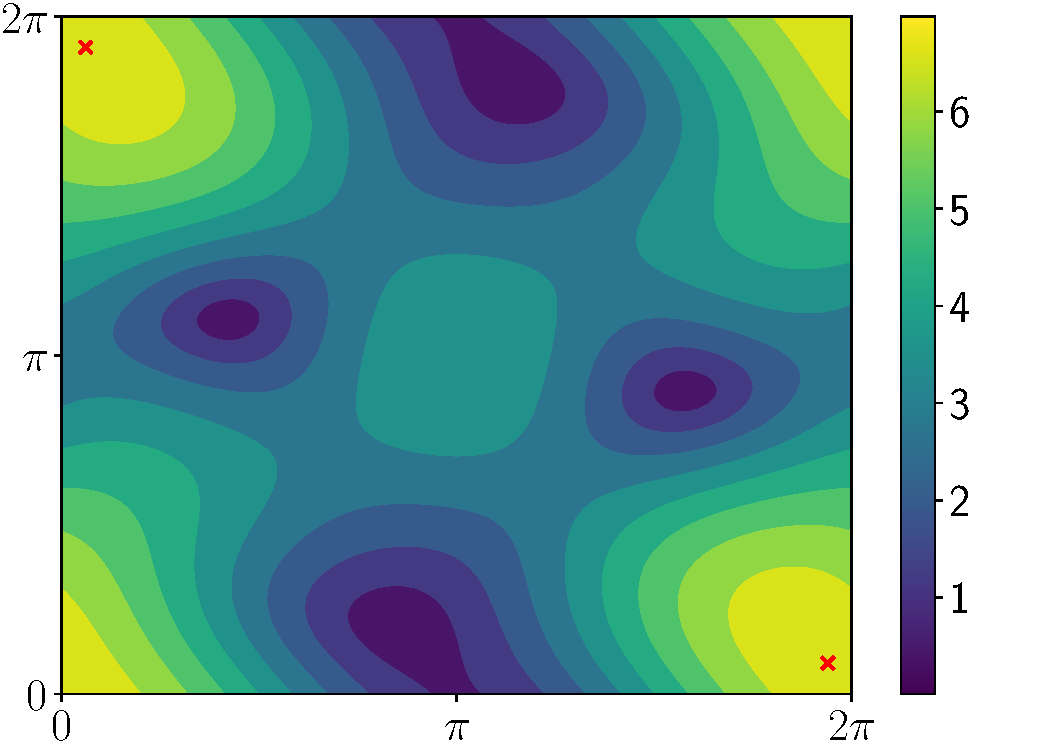
\includegraphics[scale=0.35]{figures/main/ch5-lipschitz_regularization/contour_poly_200_1_1_3.pdf}
    \caption{kernel $1\times3\times3$}
  \end{subfigure}
  \hfill
  \begin{subfigure}[b]{.49\textwidth}
    \centering
    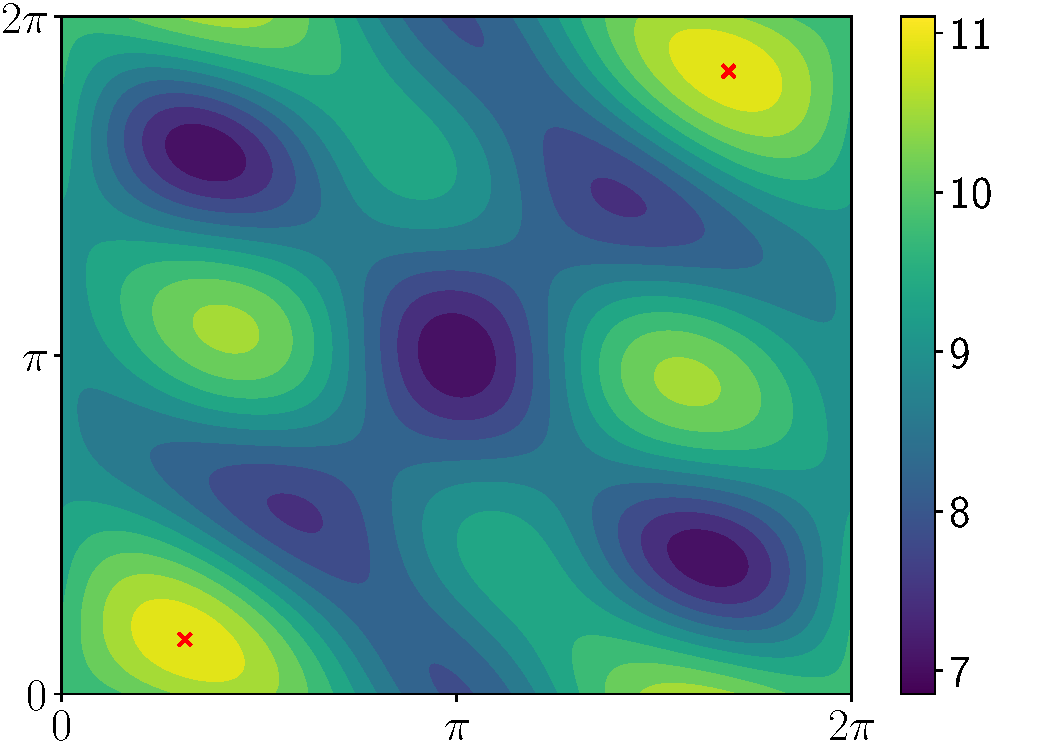
\includegraphics[scale=0.35]{figures/main/ch5-lipschitz_regularization/contour_poly_200_1_9_3.pdf}
    \caption{kernel $9\times3\times3$}
  \end{subfigure}
  \par\bigskip
  \begin{subfigure}[b]{.49\textwidth}
    \centering
    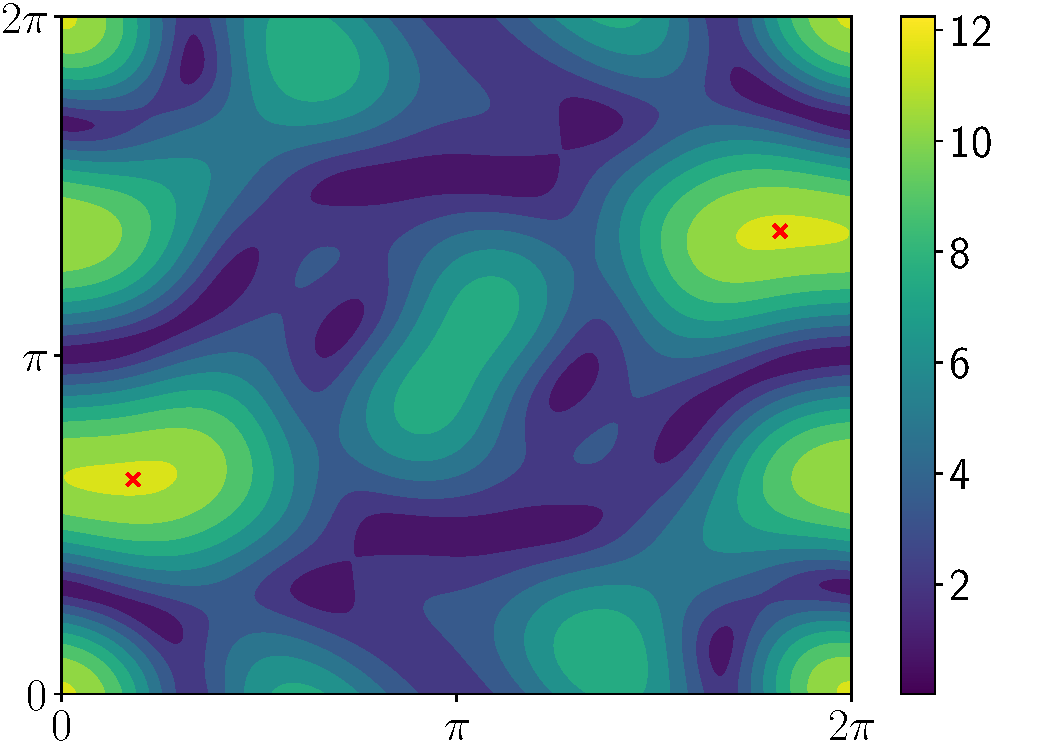
\includegraphics[scale=0.35]{figures/main/ch5-lipschitz_regularization/contour_poly_200_1_1_5.pdf}
    \caption{kernel $1\times5\times5$}
  \end{subfigure}
  \begin{subfigure}[b]{.49\textwidth}
    \centering
    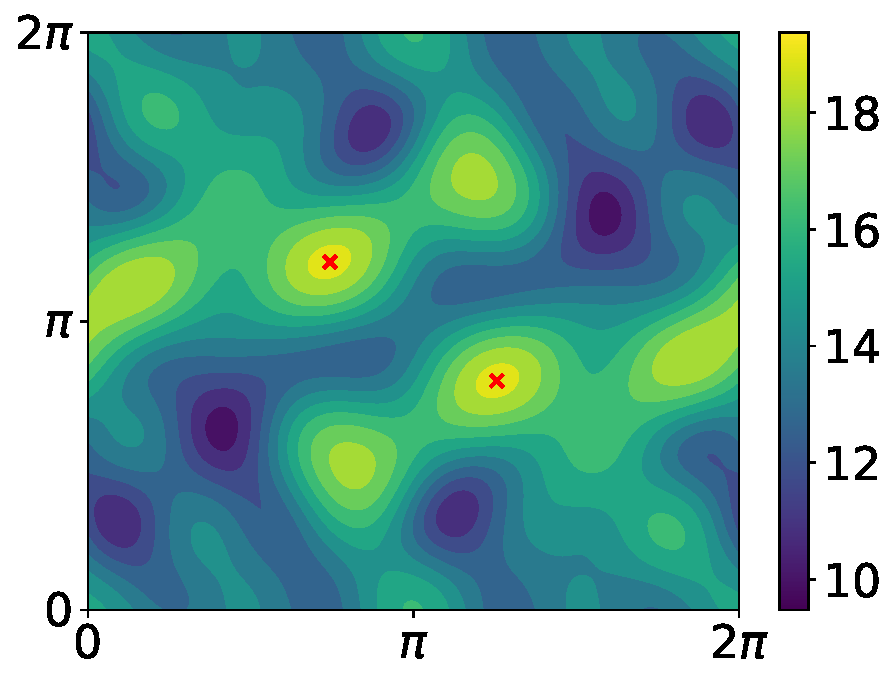
\includegraphics[scale=0.35]{figures/main/ch5-lipschitz_regularization/contour_poly_200_1_9_5.pdf}
    \caption{kernel $9\times5\times5$}
  \end{subfigure}
  \caption{Contour plots of multivariate trigonometric polynomials where the values of the coefficient are the values of a random convolutional kernel. The red dots in the figures represent the maximum modulus of the trigonometric polynomials.}
  \label{figure:contour_plot_trigonometric_polynomials}
\end{figure}%


\begin{algorithm}[htb]
  \begin{algorithmic}[1]
    \Procedure{PolyGrid}{$f, S$}\Comment{polynomial $f$, number of samples $S$}
      \State $\sigma \gets 0$, $\omega_1 \gets 0$, $\epsilon \gets \frac{2\pi}{S}$
      \For{$i=0$ \textbf{to} $S-1$}
        \State $\omega_2 \gets 0$
	\For{$j=0$ \textbf{to} $S-1$}
	  \State $\omega_2 \gets \omega_2 + \epsilon$
	  \State $\sigma \gets \max( \sigma, f(\omega_1, \omega_2))$
	\EndFor
	\State $\omega_1 \gets \omega_1 + \epsilon$
      \EndFor
      \State \textbf{return} $\sigma$ \Comment{approximated maximum modulus of $f$}
    \EndProcedure
  \end{algorithmic}
  \caption{PolyGrid Algorithm}
  \label{algorithm:ch5-polygrid}
\end{algorithm}


To fix the number of samples $S$ in the grid search, we rely on the work of~\cite{pfister2018bounding}, who has analyzed the quality of the approximation depending on $S$.
Following this work we first define $\Theta_S$, the set of $S$ equidistant sampling points as follows:
\begin{equation}
  \Theta_S \triangleq \left\{ \omega \mid \omega = k \cdot \frac{2\pi}{S} \mbox{ with }  k = 0, \dots, S-1 \right\}.
\end{equation}
Then, for a trigonometric polynomial $f: [0, 2\pi]^2 \rightarrow \Cbb$, we have:
\begin{equation}
  \max_{\omega_1, \omega_2 \in [0,2\pi]^2} \left| f(\omega_1, \omega_2) \right| \leq (1 - \alpha)^{-1} \max_{\omega_1', \omega_2' \in \Theta_S^2} \left| f(\omega_1', \omega_2') \right|,
\end{equation}
where $d$ is the degree of the polynomial and $\alpha = 2d / S$.
For a $3\times3$ kernel which gives a trigonometric polynomial of degree 1, we use $S = 10$ which gives $\alpha = 0.2$.
Using this result, we can now compute $\lipbound$ for a convolution operator with $\cout$ output channels as per \Cref{theorem:bound_sv_stacked_dbt}.
 
% The code to for computing $\lipbound$ with NumPy~\cite{numpy} and PyTorch~\cite{paszke2019pytorch} is publicly available.\footnote{\url{https://github.com/MILES-PSL/upper_bound_lipschitz_convolutional_layers}}.


%%%%%%%%%%%%%%%%%%%%%%%%%%%%%%%%%%%%%%%%%%%%%%%%%%%%%%%%%%%%%%%%%%%%%%%%%%%%%%%%
\subsection{Analysis of the Tightness of the Bound}
\label{subsection:ch2-analysis_of_the_tightness_of_the_bound}
%%%%%%%%%%%%%%%%%%%%%%%%%%%%%%%%%%%%%%%%%%%%%%%%%%%%%%%%%%%%%%%%%%%%%%%%%%%%%%%%

In this section, we study the tightness of the bound with respect to the dimensions of the doubly-block Toeplitz matrices.
For each $n \in \Nbb$, we define the matrix  $\Mmat^{(n)}$ of size $kn^2 \times n^2$ as follows:
\begin{equation}
  \Mmat^{(n)} \triangleq \textstyle \leftmat \Dmat^{(n)\top}(f_1), \dots, \Dmat^{(n)\top}(f_k) \textstyle \rightmat^\top
\end{equation}
where the matrices $\Dmat^{(n)}(f_i)$ are of size $n^2 \times n^2$. 
To analyze the tightness of the bound, we define the function $\Gamma$, which computes the difference between $\lipbound$ and the largest singular value of the function $\Mmat^{(n)}$:
\begin{equation} \label{equation:function_convergence}
  \Gamma(n) = \lipbound(\Kmat_{\Mmat^{(n)}}) - \sigma_1(\Mmat^{(n)})
\end{equation}
where $\Kmat_{\Mmat^{(n)}}$ is the convolution kernel associated with the matrix $\Mmat^{(n)}$.

\begin{figure}[ht]
  \centering
  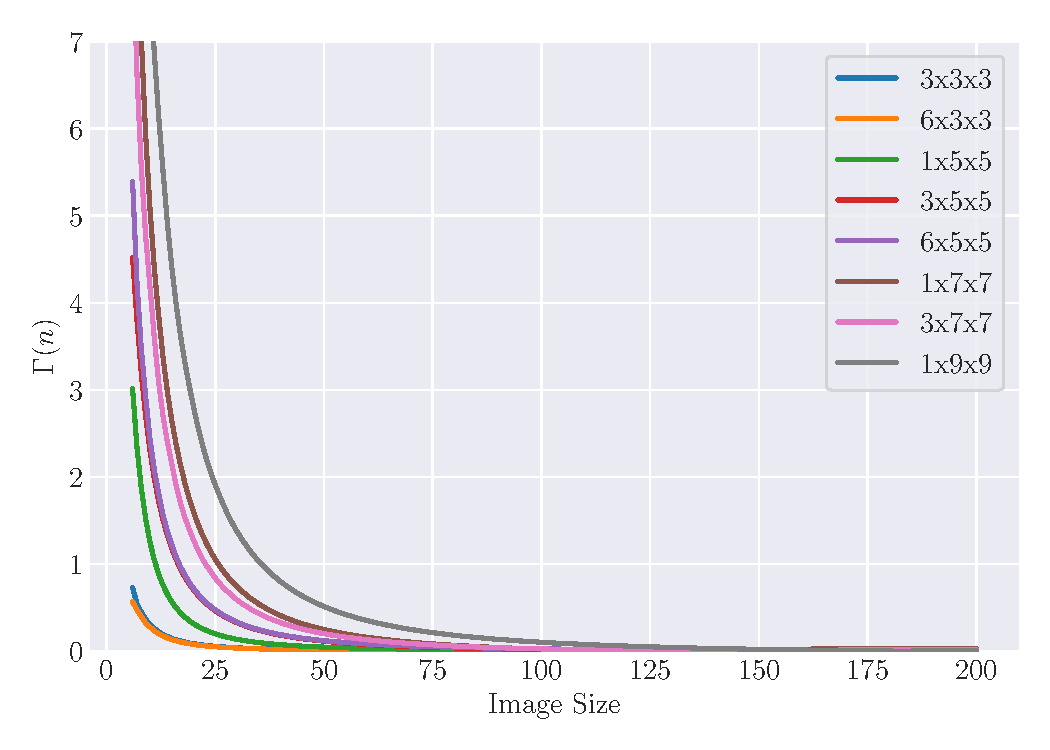
\includegraphics[width=\scalefigure\textwidth]{figures/main/ch5-lipschitz_regularization/convergence_bounds.pdf}
  \caption{Representation of the function $\Gamma(n)$ defined for different kernel size.}
  \label{figure:convergence_bound}
\end{figure}


To compute the exact largest singular value of $\Mmat^{(n)}$ for a specific $n$, we use the Implicitly Restarted Arnoldi Method (IRAM) ~\cite{lehoucq1996deflation} available in SciPy.
The results of this experiment are presented in \Cref{figure:convergence_bound}.
We observe that the difference between the bound and the actual value (approximation gap) quickly decreases as the input size increases.
For an input size of $50$, the approximation gap is as low as $0.012$ using a standard $6\times3\times3$ convolution kernel.
For a larger input size such as ImageNet ($224$), the gap is lower than $4.10^{-4}$.
Therefore $\lipbound$ gives an almost exact value of the largest singular value of the operator matrix for most realistic settings.

%%%%%%%%%%%%%%%%%%%%%%%%%%%%%%%%%%%%%%%%%%%%%%%%%%%%%%%%%%%%%%%%%%%%%%%%%%%%%%%%
\subsection{Comparison of LipBound with State-of-the-Art Approaches}
\label{subsection:ch5-comparison_of_lipbound_with_other_state-of-the-art_approaches}
%%%%%%%%%%%%%%%%%%%%%%%%%%%%%%%%%%%%%%%%%%%%%%%%%%%%%%%%%%%%%%%%%%%%%%%%%%%%%%%%

\begin{table}[ht]
  \centering
  \sisetup{%
    table-align-uncertainty=true,
    separate-uncertainty=true,
    detect-weight=true,
    detect-inline-weight=math
  }
  {\small
  \begin{tabular}%{lrccccrcccc}
    {
      lr
      S[table-format=1.3]@{\,\( \pm \)\,}S[table-format=1.3]
      S[table-format=4.2]@{\,\( \pm \)\,}S[table-format=3.2]
      r
      S[table-format=1.3]@{\,\( \pm \)\,}S[table-format=1.3]
      S[table-format=4.2]@{\,\( \pm \)\,}S[table-format=3.2]
    }
    \toprule
      &   & \multicolumn{4}{c}{\textbf{1x3x3}} &   & \multicolumn{4}{c}{\textbf{32x3x3}} \\
    \cmidrule{3-6} \cmidrule{8-11}
    &   & \multicolumn{2}{c}{\textbf{Ratio}} & \multicolumn{2}{c}{\textbf{Time (ms)}}
    &   & \multicolumn{2}{c}{\textbf{Ratio}} & \multicolumn{2}{c}{\textbf{Time (ms)}} \\
    \midrule
    \citeauthor{sedghi2018singular} &   & 0.431 & 0.042 & 1088 & 251  & & 0.666 & 0.123 & 1729 & 399 \\
    \citeauthor{singla2019bounding} &   & 1.293 & 0.126 & 1.90 & 0.48 & & 1.441 & 0.188 & 1.90 & 0.46 \\
    \citeauthor{farnia2018generalizable} &   & 0.973 & 0.006 & 4.30 & 0.64 & & 0.972 & 0.004 & 4.93 & 0.67 \\
    \midrule
    \midrule
    LipBound &  & 0.992 & 0.012 & 0.49 & 0.05 & & 0.984 & 0.021 & 0.63 & 0.46 \\
    \bottomrule
  \end{tabular}%
  }
  \caption{Comparison of the accuracy of approximation methods for computing an approximation of the largest singular value of a convolution layer.}
  \label{table:ch5-compare_bounds}%
\end{table}



\begin{table}[h]
  \centering
  \sisetup{%
    table-number-alignment=center,
    table-align-uncertainty=true,
    separate-uncertainty=true,
    detect-weight=true,
    detect-inline-weight=math
  }
  \begin{tabular}
    {
      lr
      S[table-format=4.2,table-number-alignment=right]@{\,\( \pm \)\,}S[table-format=2.2,table-number-alignment=left]
      r
      S[table-format=6.2,table-number-alignment=right]@{\,\( \pm \)\,}S[table-format=3.2,table-number-alignment=left]
      r
      S[table-format=1.2]
    }
    \toprule
    \textbf{Network} & & \multicolumn{2}{c}{\textbf{LipBound (ms)}} & & \multicolumn{2}{c}{\textbf{Power Method (ms)}} & & \textbf{Ratio} \\
    \midrule
    AlexNet & & 4.75 & 1.10 & & 38.75 & 2.52 & & 8.14 \\
    \midrule
    ResNet 18 & & 29.88 & 1.73 & & 148.35 & 14.92 & & 4.96 \\
    ResNet 34 & & 54.73 & 3.62 & & 266.85 & 25.35 & & 4.87 \\
    ResNet 50 & & 60.77 & 4.62 & & 467.61 & 36.52 & & 7.69 \\
    ResNet 101 & & 102.72 & 11.53 & & 817.06 & 102.87 & & 7.95 \\
    ResNet 152 & & 158.80 & 20.84 & & 1373.57 & 164.37 & & 8.64 \\
    \midrule
    DenseNet 121 & & 125.55 & 14.59 & &  937.35 &  11.52 & & 7.46 \\
    DenseNet 161 & & 176.11 & 19.13 & & 1292.61 &  30.50 & & 7.33 \\
    DenseNet 169 & & 188.03 & 19.74 & & 1372.62 &  21.16 & & 7.29 \\
    DenseNet 201 & & 281.13 & 23.41 & & 1930.19 & 170.79 & & 6.86 \\
    \midrule
    VGG 11 & & 13.73 & 1.19 & &  81.78 & 4.45 & & 5.95 \\
    VGG 13 & & 14.96 & 1.99 & & 102.04 & 4.20 & & 6.82 \\
    VGG 16 & & 21.92 & 1.94 & & 132.29 & 5.99 & & 6.03 \\
    VGG 19 & & 29.05 & 0.66 & & 162.28 & 4.87 & & 5.58 \\
    \midrule
    WideResNet 50-2 & & 113.28 & 45.44 & & 468.74 & 6.54 & & 4.13 \\
    \midrule
    SqueezeNet 1-0 & & 18.44 & 5.93 & & 222.40 & 25.49 & & 12.05 \\
    SqueezeNet 1-1 & & 18.26 & 6.65 & & 209.80 &  3.59 & & 11.48 \\
    \bottomrule
  \end{tabular}%
  \caption{Efficiency of LipBound computation \vs the Power Method with 10 iterations on full networks.}
  \label{table:ch5-efficiency_lipbound_full_model}%
\end{table}%

In this section we compare our PolyGrid algorithm with the values obtained using alternative approaches.
We consider the 3 alternative techniques by~\citet{sedghi2018singular,singla2019bounding,farnia2018generalizable} which have been described in \Cref{chapter:ch3-related_work}, \Cref{section:ch3-related_work_on_lipschitz_regularization}.

To compare the different approaches, we extracted 20 kernels from a trained model.
For each kernel we construct the corresponding doubly-block Toeplitz matrix and compute its largest singular value.
Then, we compute the ratio between the approximation obtained with the considered approach and the exact singular value obtained by SVD, and average the ratios over the 20 kernels.
Thus good approximations result in approximation ratios that are close to 1.
The results of this experiment are presented in \Cref{table:ch5-compare_bounds}.
The comparison has been made on a Tesla V100 GPU.
The time was computed with the PyTorch CUDA profiler and we ``warmed'' up the GPU before starting the timer for caching purposes. 

The method introduced by~\citet{sedghi2018singular} and presented in~\Cref{subsection:ch3-singular_values_of_convolutional_layers} computes the largest singular value of convolution layers based on doubly-block circulant matrices.
Doubly-block circulant matrices perform a convolution with a ``wrapping around'' operation which do not correspond to the more general setting.
We can see in \Cref{table:ch5-compare_bounds} that the values differ by an important margin.
This technique is also computationally expensive as it requires computing the SVD of $n^2$ small matrices where $n$ is the size of inputs.
\citet{singla2019bounding} have shown that the singular value of the reshape kernel is a bound on the largest singular value of the convolution layer.
Their approach is very efficient but the approximation is loose and overestimate the real value.
As said previously, the power method provides a good approximation at the expense of the efficiency.
We also compare our approach to the power method with 10 iterations from ~\citet{farnia2018generalizable} (see~\Cref{algorithm:ch3-power_method_generic}).
The results show that our proposed technique: PolyGrid algorithm can get the best of both worlds.
It achieves a near perfect accuracy while being very efficient to compute.

The results of \Cref{table:ch5-compare_bounds} shows the performance for the computation for only one convolution layer.
However, during the training Lipbound or the power method need to be computed for every layer of the network and the computation time is dependent on the architecture of the network, for example, the size of the activations or the size of the kernels.
In ~\Cref{table:ch5-efficiency_lipbound_full_model}, we compare our approach method against the power method on the full architecture, \ie, the time needed for the computation on all the layers of the networks.
We measure on the following convolutional architectures: AlexNet \cite{krizhevsky2012imagenet}, ResNet \cite{he2016deep}, DenseNet \cite{huang2017densely}, VGG \cite{simonyan2014very}, WideResNet \cite{zagoruyko2016wide}, SqueezeNet \cite{iandola2016squeezenet}.
\Cref{table:ch5-efficiency_lipbound_full_model} shows that our approach is systematically faster than the power method by a factor up to 12 when considering all the layers of the networks.
This demonstrates the scalability of our method.

% for full networks Lipbound is systematically faster than the power method by a factor up to 12.

% We also compare in~\Cref{table:ch5-efficiency_lipbound_full_model} our method against the power method of~\citet{farnia2018generalizable} on the following convolutional architectures: 







%%%%%%%%%%%%%%%%%%%%%%%%%%%%%%%%%%%%%%%%%%%%%%%%%%%%%%%%%%%%%%%%%%%%%%%%%%%%%%%%
\section{Lipschitz Regularization for Adversarial Robustness}
\label{section:ch5-lipschitz_regularization_for_adversarial_robustness}
%%%%%%%%%%%%%%%%%%%%%%%%%%%%%%%%%%%%%%%%%%%%%%%%%%%%%%%%%%%%%%%%%%%%%%%%%%%%%%%%



One promising application of Lipschitz regularization is in the area of adversarial robustness.
Empirical techniques to improve robustness against adversarial examples such as Adversarial Training only impact the training data,  and often show poor generalization capabilities~\cite{schmidt2018adversarially}.
\citet{farnia2018generalizable} have shown that the adversarial generalization error depends on the Lipschitz constant of the network, which suggests that the adversarial test error can be improved by applying Lipschitz regularization in addition to adversarial training.

In this section, we illustrate the usefulness of LipBound by training a Wide ResNet~\citep{zagoruyko2016wide} with Lipschitz regularization and adversarial training.
Our regularization scheme is inspired by the one used by \citet{yoshida2017spectral} but instead of using the power method, we use our \textbf{PolyGrid} algorithm presented in~\Cref{subsection:ch5-computing_the_maximum_modulus_of_a_trigonometric_polynomial} which efficiently computes an upper bound on the largest singular value of convolution layers.

We introduce the \textbf{AT+LipReg} loss to combine Adversarial Training and our Lipschitz regularization scheme in which layers with a large Lipschitz constant are penalized.
We consider a neural network $N_\Omega : \Xset \rightarrow \Yset$ with $\depth$ layers $\phi^{(1)}_{\Wmat^{(1)}, \bvec^{(1)}}, \dots, \phi^{(\depth)}_{\Wmat^{(\depth)}, \bvec^{(\depth)}}$ where $\Wmat^{(1)}, \dots, \Wmat^{(\depth)}$ are the weight matrices and $\Omega$ is the union of all the parameters as defined in~\Cref{definition:ch2-neural_networks}.
Given a distribution $\Dset$ over $\Xset \times \Yset$, we can train the parameters of the network by minimizing the AT+LipReg loss as follows:
\begin{equation} \label{equation:ch5-obj_function}
  \min_{\Omega} \Ebb_{\xvec,y \sim \Dset} \left[ L(N_\Omega(\xvec + \adv^{\text{adv}}_\Omega(\xvec)), y) + r(\Omega) \right]
\end{equation}
where $L$ is the cross-entropy loss function, $\adv^{\text{adv}}_\Omega(\xvec)$ is an adversarial perturbation following the loss maximization strategy presented in~\Cref{subsubsection:ch2-adversarial_attacks} and the regularization function $r$ is defined as follows:
\begin{equation}
  r(\Omega) =  C_1 \underbrace{\sum_{(\Wmat, \bvec) \in \Omega} \left( \norm{\Wmat}_\fro + \norm{\bvec}_2 \right)}_{
  \text{$\ell_2$ regularization}} + C_2 \underbrace{\vphantom{\sum_{(\Wmat, \bvec) \in \Omega}} \sum_{i=1}^{\depth-1} \log\left(\lipbound\left(\Kmat_{\Wmat^{(i)}}\right)\right)}_{\text{Lipschitz regularization}} 
\end{equation}
where $C_1$, $C_2$ are two user-defined hyper-parameters.
Note that regularizing the sum of logs is equivalent to regularizing the product of all the $\lipbound$ which is an upper bound on the global Lipschitz constant.
In practice, we also include the upper bound on the Lipschitz of the batch normalization since we can compute it very efficiently (see Appendix C.4.1 of ~\citet{tsuzuku2018lipschitz}) but we omit the last fully connected layer.

In this section, we compare the robustness of Adversarial Training~\cite{goodfellow2014explaining, madry2018towards} against the combination of Adversarial Training and Lipschitz regularization.
To regularize the Lipschitz constant of the network, we use the objective function defined in Equation~\ref{equation:ch5-obj_function}.
We train Lipschitz regularized neural networks with LipBound (see~\Cref{theorem:ch5-bound_max_sv_convolution}) implemented with PolyGrid (see~\Cref{algorithm:ch5-polygrid}) (AT+LipBound) with $S = 10$ or with the specific power method for convolutions introduced by~\citet{farnia2018generalizable} with 10 iterations (AT+PM).

Table~\ref{table:ch5-cifar_robustness} shows the gain in robustness against strong adversarial attacks across different datasets.
We can observe that both AT+LipBound and AT+PM offer a better defense against adversarial attacks and that AT+LipBound offers a further improvement over the Power Method.
\Cref{figure:ch5-attacks_pgd,figure:ch5-attacks_cw} show the Accuracy under attack with different numbers of iterations.
Table~\ref{table:ch5-results_imagenet_dataset} presents our results on the ImageNet Dataset.
First, we can observe that the AT+LipReg trained networks offer a better generalization than with standalone Adversarial Training.
Secondly, we can observe the gain in robustness against strong adversarial attacks.
Network trained with Lipschitz regularization and Adversarial Training offer a consistent increase in robustness across $\ell_\infty$ and $\ell_2$ attacks with different $\epsilon$ value.
We can also note that increasing the regularization leads to an increase in generalization and robustness.

\afterpage{
\begin{figure}[p!]
   \centering
   \begin{subfigure}[b]{\textwidth}
     \centering
     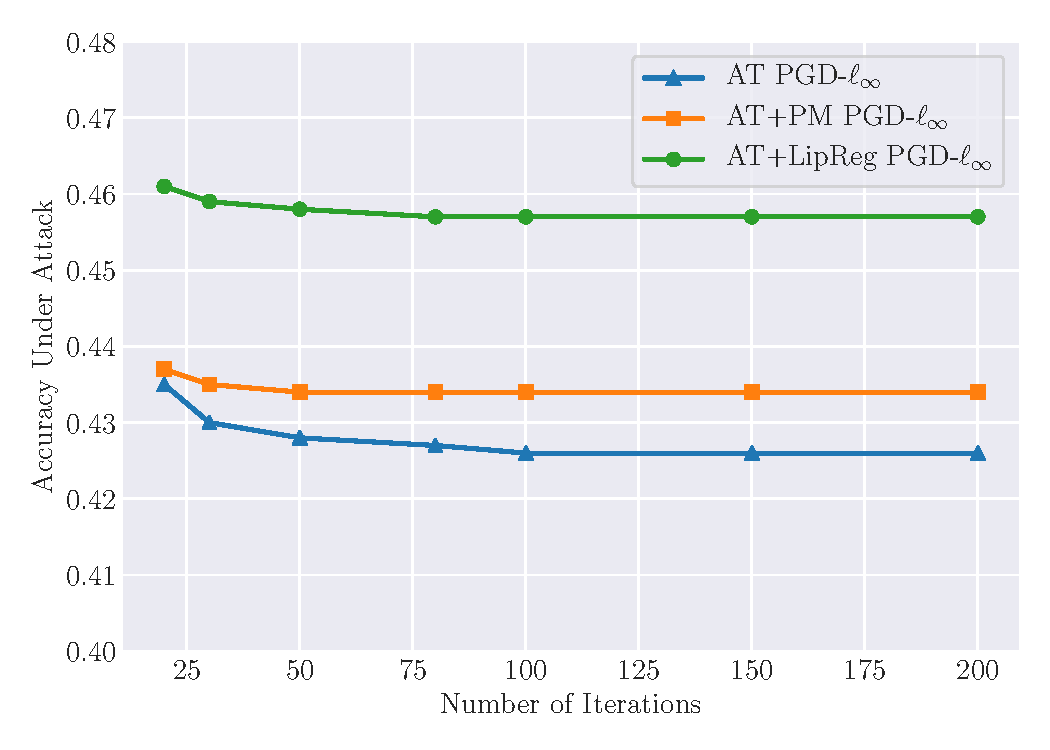
\includegraphics[width=\scalefigure\textwidth]{figures/main/ch5-lipschitz_regularization/attacks_iter_pgd.pdf}
     \caption{Robustness against $\ell_\infty$ attacks for different classifiers trained with Adversarial Training given the number of iterations.}
     \label{figure:ch5-attacks_pgd}
   \end{subfigure}
   ~\\[1cm]
   \begin{subfigure}[b]{\textwidth}
     \centering
     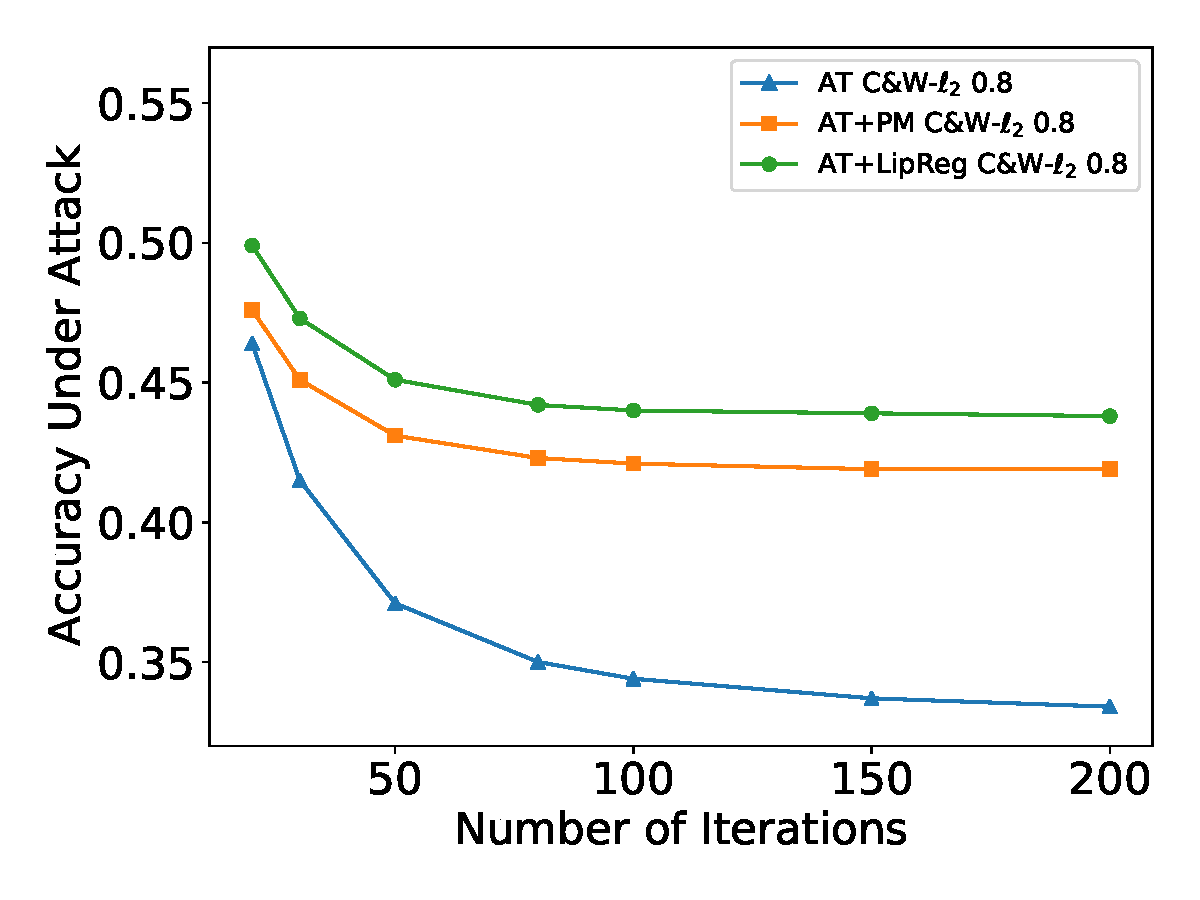
\includegraphics[width=\scalefigure\textwidth]{figures/main/ch5-lipschitz_regularization/attacks_iter_cw.pdf}
     \caption{Robustness against $\ell_\infty$ attacks for different classifiers trained with Adversarial Training given the number of iterations.}
     \label{figure:ch5-attacks_cw}
   \end{subfigure}
   ~\\[1cm]
   \caption{Accuracy under attack on CIFAR10 test set with $\ell_\infty$ and $\ell_2$ attacks for several classifiers trained with Adversarial Training given the number of iterations.}
\end{figure}
\clearpage
}


\afterpage{
\begin{figure}[p!]
   \centering
   \begin{subfigure}[b]{\textwidth}
     \centering
     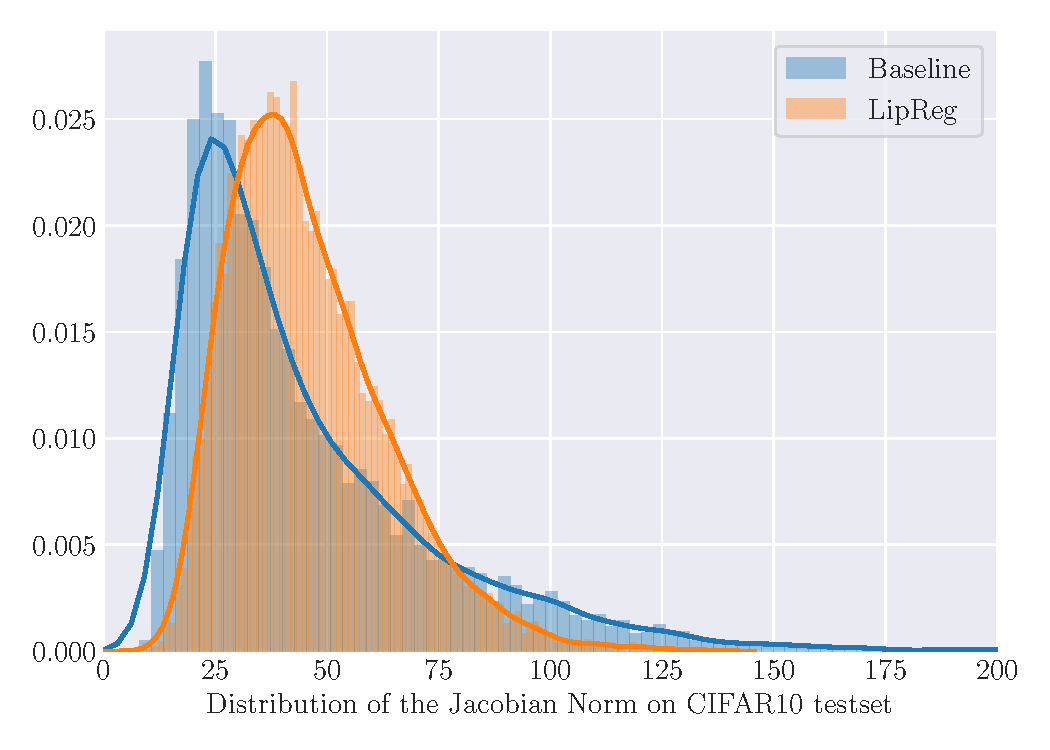
\includegraphics[width=\scalefigure\textwidth]{figures/main/ch5-lipschitz_regularization/jacobian_distribution_v1.pdf}
     \caption{Comparison of the distribution of the norm of the Jacobian of the baseline model against the model trained with Lipschitz regularization.}
     \label{figure:ch5-jacobian_distribution_v1}
   \end{subfigure}
   ~\\[1cm]
   \begin{subfigure}[b]{\textwidth}
      \centering
      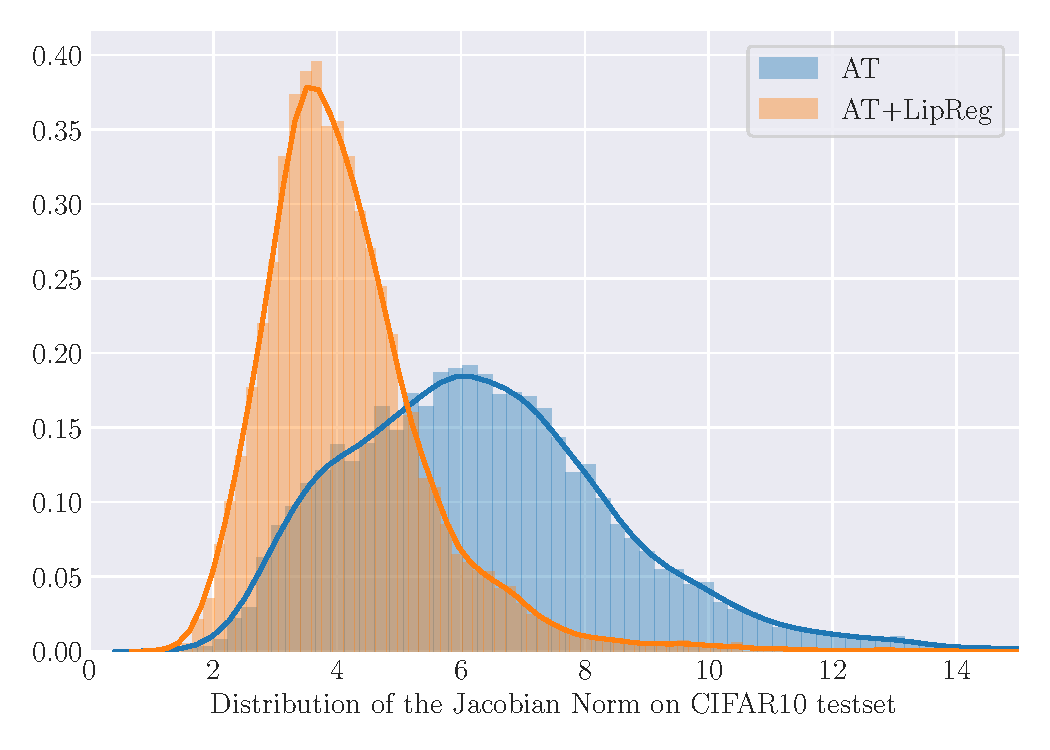
\includegraphics[width=\scalefigure\textwidth]{figures/main/ch5-lipschitz_regularization/jacobian_distribution_v2.pdf}
      \caption{Comparison of the distribution of the norm of the Jacobian of the model trained with Adversarial training against the model trained with Adversarial training and Lipschitz regularization.}
      \label{figure:ch5-jacobian_distribution_v2}
   \end{subfigure}
   ~\\[1cm]
   \caption{Distribution of the norm of the Jacobian matrix with respect to the CIFAR10 test set from a Wide ResNet trained with different schemes.} 
\end{figure}
\clearpage
}


Finally, we also conducted an experiment to study the impact of the regularization on the gradients of the whole network by measuring the norm of the Jacobian matrix, averaged over the inputs from the test set.
The results of this experiment are presented in~\Cref{figure:ch5-jacobian_distribution_v1} and show more concentrated gradients with  Lipschitz regularization, which is the expected effect.
Although Lipschitz regularization is not a Jacobian regularization, we can observe a clear shift in the distribution.
This suggests that our method does not only work layer-wise, but also at the level of the entire network.
A second experiment, using Adversarial Training, presented in~\Cref{figure:ch5-jacobian_distribution_v2} demonstrates that the effect is even stronger when the two techniques are combined together.
% This corroborates the work by~\citet{farnia2018generalizable}.
It also demonstrates that Lipschitz regularization and Adversarial Training (or other Jacobian regularization techniques) are complementary.
Hence they offer an increased robustness to adversarial attacks as demonstrated above.


\begin{table}[t]
  \sisetup{%
    table-align-uncertainty=true,
    separate-uncertainty=true,
    detect-weight=true,
    detect-inline-weight=math
  }
  \centering
  \begin{subfigure}[b]{\textwidth}
    \begin{tabular}
      {
	l
        S[table-format=1.3]@{\,\( \pm \)\,}S[table-format=1.3]
        S[table-format=1.3]@{\,\( \pm \)\,}S[table-format=1.3]
        S[table-format=1.3]@{\,\( \pm \)\,}S[table-format=1.3]
        S[table-format=1.3]@{\,\( \pm \)\,}S[table-format=1.3]
      }
      \toprule
      \textbf{Model} & \multicolumn{2}{c}{\textbf{Accuracy}} & \multicolumn{2}{c}{\textbf{PGD-$\ell_\infty$}}
      & \multicolumn{2}{c}{\textbf{C\&W-$\ell_2$ 0.6}} & \multicolumn{2}{c}{\textbf{C\&W-$\ell_2$ 0.8}} \\
      \midrule
      \textbf{Baseline} & \textbf{0.953} & 0.001 & 0.000 & 0.000 & 0.002 & 0.000 & 0.000 & 0.000 \\
      \textbf{AT}       & 0.864 & 0.001 & 0.426 & 0.000 & 0.477 & 0.000 & 0.334 & 0.000 \\
      \textbf{AT+PM}    & 0.788 & 0.010 & 0.434 & 0.007 & 0.521 & 0.005 & 0.419 & 0.003 \\
      \textbf{AT+LipReg} & 0.808 & 0.022 & \textbf{0.457} & 0.002 & \textbf{0.547} & 0.022 & \textbf{0.438} & 0.020 \\
      \bottomrule
    \end{tabular}%
    \caption{Results on CIFAR10 dataset}
    \label{subfigure:ch5-results_cifar10_data}
  \end{subfigure}
  \par\bigskip
  \begin{subfigure}[b]{\textwidth}
    \begin{tabular}
      {
	l
        S[table-format=1.3]@{\,\( \pm \)\,}S[table-format=1.3]
        S[table-format=1.3]@{\,\( \pm \)\,}S[table-format=1.3]
        S[table-format=1.3]@{\,\( \pm \)\,}S[table-format=1.3]
        S[table-format=1.3]@{\,\( \pm \)\,}S[table-format=1.3]
      }
      \toprule
      \textbf{Model} & \multicolumn{2}{c}{\textbf{Accuracy}} & \multicolumn{2}{c}{\textbf{PGD-$\ell_\infty$}}
      & \multicolumn{2}{c}{\textbf{C\&W-$\ell_2$ 0.6}} & \multicolumn{2}{c}{\textbf{C\&W-$\ell_2$ 0.8}} \\
      \midrule
      \textbf{Baseline} & \textbf{0.792} & 0.000  & 0.000 & 0.000  & 0.001 & 0.000  & 0.000 & 0.000 \\
      \textbf{AT} & 0.591 & 0.000  & 0.199 & 0.000  & 0.263 & 0.000  & 0.183 & 0.000 \\
      \textbf{AT+LipReg} & 0.552 & 0.019  & \textbf{0.215} & 0.004  & \textbf{0.294} & 0.010  & \textbf{0.226} & 0.008  \\
      \bottomrule
    \end{tabular}%
    \caption{Results on CIFAR100 dataset}
    \label{subfigure:ch5-results_cifar100_data}
  \end{subfigure}
  \caption{Accuracy under $\ell_2$ and $\ell_\infty$ attacks of different training schemes on CIFAR10/100 datasets.} 
% We compare vanilla Adversarial Training with the combination of Lipschitz regularization and Adversarial Training. We also compare the effectiveness of the power method by~\citet{farnia2018generalizable} and $\lipbound$. We fix the parameter $\lambda_2$ from \Cref{equation:ch5-obj_function}) to $0.008$ for AT+PM and AT+LipReg. It has been chosen from a grid search among 10 values. The attacks are computed with 200 iterations. }
  \label{table:ch5-cifar_robustness}%
\end{table}%


\begin{table}[t]
  \centering
  \tabcolsep=1.9mm
  {\small
  \begin{tabular}{
    lc
    c
    cc
    c
    ccc
  }
    \toprule
    \multicolumn{1}{c}{\multirow{2}[4]{*}{\textbf{Model}}} & \multicolumn{1}{c}{\multirow{2}[4]{*}{\textbf{Natural}}} &  
    & \multicolumn{2}{c}{\textbf{PGD}-$\ell_\infty$} &   & \multicolumn{3}{c}{\textbf{C\&W}-$\ell_2$} \\
    \cmidrule{4-5}\cmidrule{7-9} 
    &  &  & \multicolumn{1}{c}{0.02} & \multicolumn{1}{c}{0.031} &   & \multicolumn{1}{c}{1.00} & \multicolumn{1}{c}{2.00} & \multicolumn{1}{c}{3.00} \\
    \midrule
    \textbf{Baseline} \cite{he2016deep} & \textbf{0.782} & & 0.000 & 0.000 & & 0.000 & 0.000 & 0.000 \\
    \textbf{AT} & 0.509 &   & 0.251 & 0.118 &   & 0.307 & 0.168 & 0.099 \\
    \textbf{AT+LipReg} ($C_2 = 0.0006$) & \textbf{0.515} &   & \textbf{0.255} & \textbf{0.121} &   & \textbf{0.316} & \textbf{0.177} & \textbf{0.105} \\
    \textbf{AT+LipReg} ($C_2 = 0.0010$) & \textbf{0.519} &   & \textbf{0.259} & \textbf{0.123} &   & \textbf{0.338} & \textbf{0.204} & \textbf{0.129} \\
    \bottomrule
  \end{tabular}%
  }
  % \caption{This table shows the accuracy and accuracy under $\ell_2$ and $\ell_\infty$ attack of ImageNet dataset. We compare Adversarial Training with the combination of Lipschitz regularization and Adversarial Training \cite{madry2018towards}. }
  \caption{Natural accuracy and accuracy under $\ell_2$ and $\ell_\infty$ attacks of different training schemes on the ImageNet dataset.} 
  \label{table:ch5-results_imagenet_dataset}
\end{table}%





\paragraph{Experimental Settings CIFAR10/100 Dataset.}
For all our experiments, we use the Wide ResNet architecture introduced by~\citet{zagoruyko2016wide} to train our classifiers.
We use Wide ResNet networks with 28 layers and a width factor of 10.
We train our networks for 200 epochs with a batch size of $200$.
We use Stochastic Gradient Descent with a momentum of $0.9$, an initial learning rate of $0.1$ with exponential decay of 0.1 (MultiStepLR gamma = 0.1) after the epochs $60$, $120$ and $160$.
For Adversarial Training ~\cite{madry2018towards}, we use Projected Gradient Descent with an $\epsilon = 8/255 (\approx 0.031)$, a step size of $\epsilon/5 (\approx 0.0062)$ and 10 iterations, we use a random initialization but run the attack only once.
To evaluate the robustness of our classifiers, we rigorously followed the experimental protocol proposed by~\citet{carlini2019evaluating,tramer2020adaptive}.
More precisely, as an $\ell_\infty$ attack, we use PGD with the same parameters ($\epsilon = 8/255$, a step size of $\epsilon/5$) but we increase the number of iterations up to 200 with 10 restarts.
For each image, we select the perturbation that maximizes the loss among all the iterations and the 10 restarts.
As $\ell_2$ attacks, we use a bounded version of the~\citet{carlini2017towards} attack.
We choose $0.6$ and $0.8$ as bounds for the $\ell_2$ perturbation.
Note that the $\ell_2$ ball with a radius of $0.8$ has approximately the same volume as the $\ell_\infty$ ball with a radius of $0.031$ for the dimensionality of CIFAR10/100.


\paragraph{Experimental Settings for ImageNet Dataset.}
For all our experiments, we use the ResNet-101 architecture \cite{he2016deep}.
We have used Stochastic Gradient Descent with a momentum of $0.9$, a weight decay of $0.0001$, label smoothing of $0.1$, an initial learning rate of $0.1$ with exponential decay of $0.1$ (MultiStepLR gamma = $0.1$) after the epochs $30$ and $60$.
We have used Exponential Moving Average over the weights with a decay of $0.999$.
We have trained our networks for 80 epochs with a batch size of $4096$.
For Adversarial Training, we have used PGD with 5 iterations, $\epsilon = 8/255 (\approx 0.031)$ and a step size of $\epsilon/5 (\approx 0.0062)$.
To evaluate the robustness of our classifiers on ImageNet Dataset, we have used an $\ell_\infty$ and an $\ell_2$ attacks.
More precisely, as an $\ell_\infty$ attack, we use PGD with an epsilon of 0.02 and 0.031, a step size of $\epsilon/5$) with a number of iterations to 30 with 5 restarts.
For each image, we select the perturbation that maximizes the loss among all the iterations and the 10 restarts.
As $\ell_2$ attacks, we use a bounded version of the~\citet{carlini2017towards} attack.
We have used $1$, $2$ and $3$ as bounds for the $\ell_2$ perturbation.


%%%%%%%%%%%%%%%%%%%%%%%%%%%%%%%%%%%%%%%%%%%%%%%%%%%%%%%%%%%%%%%%%%%%%%%%%%%%%%%%
\section{Concluding Remarks}
\label{section:ch5-concluding_remarks}
%%%%%%%%%%%%%%%%%%%%%%%%%%%%%%%%%%%%%%%%%%%%%%%%%%%%%%%%%%%%%%%%%%%%%%%%%%%%%%%%

In this chapter, we introduced a new bound on the Lipschitz constant of convolution layers that is both accurate and efficient to compute.
We used this bound to regularize the Lipschitz constant of neural networks and demonstrated its computational efficiency in training large neural networks with a regularized Lipschitz constant.
As an illustrative example, we combined our bound with adversarial training, and showed that this increases the robustness of the trained networks to  adversarial attacks.
The scope of our results goes beyond this application and can be used in a wide variety of settings, for example, to stabilize the training of Generative Adversarial Networks (GANs) and invertible networks, or to improve generalization capabilities of classifiers.


  %%%%%%%%%%%%%%%%%%%%%%%%%%%%%%%%%%%%%%%%%%%%%%%%%%%%%%%%%%%%%%%%%%%%%%%%%%%%%%%%
\chapter{Conclusion}
\label{chapter:ch6-conclusion}
%%%%%%%%%%%%%%%%%%%%%%%%%%%%%%%%%%%%%%%%%%%%%%%%%%%%%%%%%%%%%%%%%%%%%%%%%%%%%%%%
\localtoc

%%%%%%%%%%%%%%%%%%%%%%%%%%%%%%%%%%%%%%%%%%%%%%%%%%%%%%%%%%%%%%%%%%%%%%%%%%%%%%%%
\section{Summary of the Contributions}
\label{section:ch6-summary_of_the_contributions}
%%%%%%%%%%%%%%%%%%%%%%%%%%%%%%%%%%%%%%%%%%%%%%%%%%%%%%%%%%%%%%%%%%%%%%%%%%%%%%%%


State-of-the-art in a variety of domains, deep neural networks exhibit important limitations.
Indeed, current neural networks tend to be very large in terms of their number of parameters which make them difficult to train and to deploy in real-world applications.
Furthermore, they exhibit instability to small perturbations of their inputs which lead to adversarial attacks. 

In this thesis, we have used structured matrices from the Toeplitz family to make contributions to the field of deep learning.
Our contributions are twofold.
First, we studied deep diagonal-circulant neural networks, which are deep neural networks in which weight matrices are the product of diagonal and circulant ones.
Using diagonal and circulant matrices instead of dense ones allows for an important reduction in the number of parameters which make them more efficient and cost-effective.
In addition to being more compact than fully connected neural networks, diagonal-circulant neural networks have a high expressivity that makes them useful for numerous use cases.
In order to characterize the expressive power of diagonal-circulant neural networks, we build upon the work of~\citet{huhtanen2015factoring} which states that any matrix can be decomposed into a product of alternating diagonal and circulant matrices.
Based on this result, we have successfully demonstrated that neural networks with diagonal and circulant matrices are \emph{universal approximators} and characterized their expressive power with respect to their depth.
We also demonstrated the effectiveness of this class of compact neural networks to video classification with a real-world dataset.

% Secondly, we study the properties of doubly-block Toeplitz matrices which are the matrix equivalent of the convolution operation. 
% Using the properties of this type of structured matrix allows us to develop a new regularization scheme of convolutional neural networks that improve their robustness against adversarial attacks.
% This regularization scheme reduces a bound of the Lipschitz constant of the neural networks thus making it less sensitive to small perturbations of its input.

% From the properties of doubly-block Toeplitz matrices and a Fourier representation introduced by~\citet{grenander1958toeplitz}, we demonstrated an upper-bound on the singular values of convolution layers.
% In order to use this upper-bound in a large-scale setting, we introduce the PolyGrid algorithm (see \Cref{algorithm:ch5-polygrid}) which efficiently and accurately computes an approximation of this upper-bound.
% Finally, we demonstrated that employing this bound as a regularizer improved the generalization and the robustness of neural networks trained with the adversarial training scheme.
%
% ---

Secondly, we study the properties of doubly-block Toeplitz matrices which are the matrix equivalent of the convolution operation. 
Using the properties of this type of structured matrix and a Fourier representation introduced by~\citet{grenander1958toeplitz}, we demonstrated an upper-bound on the singular values of convolution layers leading to a new regularization scheme of convolutional neural networks that improve their robustness against adversarial attacks.
In order to use this upper-bound in a large-scale setting, we introduced the PolyGrid algorithm (see \Cref{algorithm:ch5-polygrid}) which efficiently and accurately computes an approximation of this upper-bound.
Finally, we demonstrated that employing this bound as a regularizer reduces the sensitivity of the network to small perturbations, thus, improving the generalization and the robustness of the network.



% This regularization scheme reduces a bound of the Lipschitz constant of the neural networks thus making it less sensitive to small perturbations of its input.



% Secondly, we proposed a contribution based on the observation that the convolution operation of convolution layers can be interpreted as a matrix-multiplication where the matrix is the concatenation of multiple doubly-block Toeplitz matrices.
%
% a new regularization scheme of convolutional neural networks that improve their robustness against adversarial attacks.
%
% This contribution is based 




%%%%%%%%%%%%%%%%%%%%%%%%%%%%%%%%%%%%%%%%%%%%%%%%%%%%%%%%%%%%%%%%%%%%%%%%%%%%%%%%
\section{Perspectives and Future Works}
\label{section:ch6-perspectives_and_future_works}
%%%%%%%%%%%%%%%%%%%%%%%%%%%%%%%%%%%%%%%%%%%%%%%%%%%%%%%%%%%%%%%%%%%%%%%%%%%%%%%%

\subsection{Designing Compact Transformers for Natural Language Processing}


In order to improve upon our work on compact neural networks, one idea follows naturally.
The race towards larger convolutional neural networks seemed to have slowed following the work of \citet{tan2019efficientnet} which devised compact state-of-the-art neural networks for image recognition.
However, other types of architecture, \eg, \emph{Transformers} which rely heavily on dense matrices, have seen their number of parameters exploding in recent years.
The latest model which was designed by \citet{fedus2021switch} has 1 trillion parameters, 5.7 times than the second largest, proposed by \citet{brown2020language}, which had 175 billion parameters.

In~\Cref{chapter:ch4-diagonal_circulant_neural_network} and Appendix~\ref{appendix:ap2-diagonal_circulant_neural_networks_for_video_classification}, we have used the diagonal-circulant decomposition for compressing embedding layers in the context of video classification.
This decomposition could also be used to compress attention layers of Transformers networks~\cite{vaswani2017attention} where the attention layer is described as follows:
\begin{equation}
  \text{Attention}(\Qmat, \Kmat, \Vmat) = \text{softmax} \left( \frac{\Qmat \Kmat^\top}{\sqrt{d_k}} \right) \Vmat \enspace,
\end{equation}
where $\Qmat, \Kmat$ and $\Vmat$ are dense matrices.
Taking this layer as a building block leads to large neural networks as demonstrated by the GPT-3 architecture with 96 attention layers and 175 billion parameters.
Although, the diagonal-circulant decomposition could successfully reduce the number of parameters of attention layers, it may have limited impact on \emph{multi-head attention layers} which are a concatenation of small attention layers due to the reduced dimension of each matrix.
% , the total number of parameters is similar to that of single-head attention with full dimensionality.
% \begin{align}
%   \text{MultiHead}(\Qmat, \Kmat, \Vmat) &= \text{concat}(\Hmat^{(1)}, \dots, \Hmat^{(h)}) \Wmat_O \\
%   \text{where } \Hmat^{(i)} &= \text{Attention}(\Qmat \Wmat^{(i)}_Q, \Kmat \Wmat^{(i)}_K, \Vmat \Wmat^{(i)}_V) 
% \end{align}
% where $\Wmat^{(i)}_Q$, $\Wmat^{(i)}_K$ and $\Wmat^{(i)}_V$ are projection matrices.
% Due to the reduced dimension of each matrix of the multi-head attention layer, the total number of parameters is similar to that of single-head attention with full dimensionality.



% ---------------
%
% \todotext{update here}
%
% The regularization of the Lipschitz constant of neural networks has been a growing interest in the training of neural networks.
% Indeed, Lipschitz regularization goes beyond robustness of neural networks and can be used in a wide variety of settings, for example, to stabilize the training of Generative Adversarial Networks and invertible networks, or to improve generalization capabilities of classifiers.
%
%
% Currently, 
%
% It is important to note that the result achieved by combining adversarial training and Lipschitz regularization allow an improvement of 
%
% and devising techniques to better control the expressiveness of neural network is  



\subsection{Regularization on the Condition Number of Convolution Layers}


In \Cref{chapter:ch5-lipschitz_bound}, we have proposed an upper bound on the largest singular value of convolution layers which allow us to regularize the Lipschitz constant of the network thus improving the robustness.
% Indeed, a Lipschitz regularization during training combined with a local smoothing technique such as adversarial training allow an important gain in robustness. 
However, an important reduction of the Lipschitz constant prevents the network from learning correctly. 
Indeed, as demonstrated by the work of \cite{zhang2019theoretically}, accuracy and robustness are actually at odds, meaning that improving the robustness (\ie in our case, reducing the expressivity) hurts the training and the natural accuracy of the network. 
In our experiments, the phenomenon called \emph{rank collapse} \cite{saxe2014exact} where the rank of the weights matrices tend to decrease during training combined with a strong Lipschitz regularization would prevent convergence.
% as the expressivity is concentrated in the singular vector associated with the largest singular values.
An interesting solution would be to regularize the largest singular value and promoting the smallest in order to promote orthogonality.
% regularize the condition number of the weight matrices (ratio between the highest and lowest singular values).
The following bound on the condition number of general matrices \citet{guggenheimer1995simple} could be studied:
\begin{equation}
  \kappa(\Wmat) \le \frac{2}{\abs{\det(\Wmat)}} \left(\frac{\norm{\Amat}_\fro}{\sqrt{r}}\right)^r
\end{equation}
where $r$ is the rank of $\Wmat$.
As such, using the bound as a regularizer will encourage the orthogonality, just like a layer normalization.
Therefore, we could design some heuristic regularizers to encourage a smaller $\left(\frac{\norm{\Wmat}_\fro}{\sqrt{r}}\right)^r$ and larger $\abs{\det(\Wmat)}$ separately, as given by the following objective function: 
\begin{align} 
  \min_{\Omega} \Ebb_{\xvec, y \sim \Dset} \left[ L(N_\Omega(\xvec), y)  + C_1 \sum_{i=1}^\depth \norm{\Wmat^{(i)}}_\fro + C_2 \sum_{i=1}^{\depth} \abs{\det(\Wmat^{(i)})} \right]
\end{align}
where the determinant of doubly-block Toeplitz matrices under some assumption could be expressed with the Szeg\"{o} Theorem \cite{szego1915grenzwertsatz} and can be approximated with the help of \emph{Random Matrix Theory} \cite{basor2017asymptotics}.

% \subsection{Stronger Provably Adversarial Robustness with Noise Injection and Lipschitz Regularization}
%
% xxx
%
% In Appendix xxx, we have shown that injecting random noise from the Exponential family both during training and inference phases provably defend against adversarial attacks.
% In our experimental  
%






\subsection{Going Beyond the Lipschitz Constant} 

Finally, in order to better understand the behavior of neural networks and the transformation they perform, it would be interesting to go beyond the Lipschitz constant and consider their full spectrum.
Indeed, the spectrum of a linear map is a set that contains the eigenvalues and can be seen as a description of the properties and behavior of the operator.
For example, for a linear operator $\Lmat: \Xset \rightarrow \Xset$, the spectrum gives precise information on the solvability of the following linear equation
\begin{equation}
  \lambda \xvec - \Lmat \xvec = \yvec
\end{equation}
It is natural to ask if we could define a spectrum that equivalently gives information on the following nonlinear equation
\begin{equation}
  \lambda \xvec - \Fmat(\xvec) = \yvec \enspace.
\end{equation}

In this line of research, \citet{kachurovskii1969regular} have defined a spectrum for nonlinear continuous Lipschitz operators which share important properties with the spectrum of linear operators.
More precisely, let $\Fmat: \Xset \rightarrow \Xset$ be a nonlinear continuous Lipschitz map, the \emph{Kachurovskij spectrum} of $\Fmat$ is given by
\begin{equation}
  \sigma(\Fmat) \triangleq \left\{ \lambda \in \Cbb \mid \lambda \Imat - f \text{ is not a lipeomorphism} \right\} 
\end{equation} 
where a nonlinear Lipschitz continuous operator is a \emph{lipeomorphism} if its inverse is also nonlinear Lipschitz continuous.
We can also define the complement of the spectrum, \ie, the \emph{Kachurovskij resolvent set} as follows: 
\begin{equation}
  \mu(\Fmat) \triangleq \Cbb \setminus \mu(\Fmat) 
\end{equation}
The resolvent set can be seen as the set of complex numbers for which the operator is \emph{well behaved}.
The Kachurovskij spectrum is a compact subset of the complex plane but may be empty.
Kachurovskij have also shown that the emptiness of this spectrum can be prevented if we restrict ourselves to nonlinear continuous Lipschitz operators that admit a Fréchet-derivative $\Fmat'(\xvec_0)$ at some point $\xvec_0 \in \Xset$.
In this case, the Kachurovskij spectrum share all the properties of a linear operator which are: closed, compact, bounded and non-empty. 

Neural networks are differentiable nonlinear Lipschitz continuous functions, therefore the study of the Kachurovskij spectrum could give important insight on their stability, invertibility and robustness to adversarial examples.



%%%%%%%%%%%%%%%%%%%%%%%%%%%%%%%%%%%%%%%%%%%%%%%%%%%%%%%%%%%%%%%%%%%%%%%%%%%%%%%%
\section{Discussion}
\label{section:ch6-discussion}
%%%%%%%%%%%%%%%%%%%%%%%%%%%%%%%%%%%%%%%%%%%%%%%%%%%%%%%%%%%%%%%%%%%%%%%%%%%%%%%%


% The global regularization of neural network during training combined with a local smoothing technique such as adversarial training allow an important gain in robustness. 
% However, our contribution also highlight some important difficulties in training neural networks.


Although our contributions offer concrete techniques for building compact and reliable neural networks, they also highlight some important difficulties in training neural networks. 
First, if we discard techniques such as pruning or quantization for building compact neural networks due to the necessity of training a large neural network prior to compression, designing parameters-efficient neural networks that are compact \emph{by nature} require rethinking the whole architecture.
For computer vision tasks, the convolution operation is a compact and powerful transform, however, we still haven't found such equivalent transforms for other use cases.
Although the multi-head attention layer is more efficient than the attention layer for NLP tasks, using this type of transform in a neural network is still very parameter-hungry as demonstrated by the recent state-of-the-art for language models \cite{brown2020language}.


Secondly, defense techniques against adversarial attacks have shown great improvements in the last few years.
However, with current state-of-the-art techniques, it is still difficult to reach an accuracy higher than 60\% on a CIFAR10 (which is considered a small dataset) and the accuracy decreases further on datasets with a larger dimensionality.
Consequently, building robust neural networks still remain very much an open question.
We believe that further breakthroughs in this area will come as a by-product on research on \emph{understanding neural networks}. 
Accordingly, we hope that our contribution to the understanding of diagonal-circulant and convolution neural networks is a small step in this direction.



% while new techniques successfully improve the robustness of neural networks, it has been shown that accuracà and robustness are actually at odds \cite{zhang2019theoretically}, 











  % \chapter{Appendix} \label{chapter:appendix}


  % Appendix
  % \renewcommand\appendixpagename{\usekomafont{disposition}Appendices}
  % \begin{appendices}
  %   \renewcommand\chaptername{Appendix}
  %   %%%%%%%%%%%%%%%%%%%%%%%%%%%%%%%%%%%%%%%%%%%%%%%%%%%%%%%%%%%%%%%%%%%%%%%%%%%%%%%
\chapter{Generalization of Widom Identity}
\label{appendix:ap1-proof_of_the_generalization_of_widom_identity}
%%%%%%%%%%%%%%%%%%%%%%%%%%%%%%%%%%%%%%%%%%%%%%%%%%%%%%%%%%%%%%%%%%%%%%%%%%%%%%%
% \localtoc

\todotext{introduce this appendix}
\emph{XXX}


\begin{proof}[\Cref{lemma:ch5-widom_idenity}]
Let $(i, j)$ be matrix indexes such $(\ \cdot\ )_{i, j}$ correspond to the value at the $i^\textrm{th}$ row and $j^\textrm{th}$ column, let us define the following notation:
\begin{align*}
    i_1 &= \left\lfloor i/n \right\rfloor \quad \quad &&j_1 = \left\lfloor j/n \right\rfloor \\
    i_2 &= i \mod n \quad \quad &&j_2 = j \mod n
\end{align*}

Let us define $\hat{f}$ as the 2 dimensional Fourier transform of the function $f$. We refer to $\hat{f}_{h_1, h_2}$ as the Fourier coefficient indexed by $(h_1, h_2)$ where $h_1$ correspond to the index of the block of the doubly-block Toeplitz and $h_2$ correspond to the index of the value inside the block. More precisely, we have 
\begin{align}
    \leftmat \Dmat(f) \rightmat_{i, j} &= \hat{f}_{(\left\lfloor j/n \right\rfloor - \left\lfloor i/n \right\rfloor), ((j \mod n) - (i \mod n)))} \label{equation:expression_fourier} \\
    \leftmat \Hmat^{\alpha_0}(f) \rightmat_{i, j} &= \hat{f}_{(\left\lfloor j/n \right\rfloor + \left\lfloor i/n \right\rfloor + 1), ((j \mod n) - (i \mod n)))} \\
    \leftmat \Hmat^{\alpha_1}(f) \rightmat_{i, j} &= \hat{f}_{(\left\lfloor j/n \right\rfloor - \left\lfloor i/n \right\rfloor), ((j \mod n) + (i \mod n) + 1))} \\
    \leftmat \Hmat^{\alpha_2}(f) \rightmat_{i, j} &= \hat{f}_{(\left\lfloor j/n \right\rfloor - \left\lfloor i/n \right\rfloor), ((j \mod n) - (i \mod n)))} \\
    \leftmat \Hmat^{\alpha_3}(f) \rightmat_{i, j} &= \hat{f}_{(\left\lfloor j/n \right\rfloor + \left\lfloor i/n \right\rfloor + n), ((j \mod n) + (i \mod n) + 1))}
\end{align}

We simplify the notation of the expressions above as follow:
\begin{align}
    \leftmat \Dmat(f) \rightmat_{i, j} &= \hat{f}_{(j_1 - i_1), (j_2 - i_2 )} \\
    \leftmat \Hmat^{\alpha_0}(f) \rightmat_{i, j} &= \hat{f}_{(j_1 + i_1 + 1), (j_2 - i_2 )} \\
    \leftmat \Hmat^{\alpha_1}(f) \rightmat_{i, j} &= \hat{f}_{(j_1 - i_1), (j_2 + i_2 + 1)} \\
    \leftmat \Hmat^{\alpha_2}(f) \rightmat_{i, j} &= \hat{f}_{(j_1 - i_1), (j_2 - i_2 )} \\
    \leftmat \Hmat^{\alpha_3}(f) \rightmat_{i, j} &= \hat{f}_{(j_1 + i_1 + n), (j_2 + i_2 + 1)}
\end{align}

The convolution theorem states that the Fourier transform of a product of two functions is the convolution of their Fourier coefficients. Therefore, one can observe that the entry $(i, j)$ of the matrix $\Dmat(f g)$ can be express as follows:

\begin{equation*}
    \leftmat \Dmat(f g) \rightmat_{i, j} = \sum_{k_1 = -2n + 1}^{2n-1} \sum_{k_2 = -2n + 1}^{2n-1} \hat{f}_{(k_1-i_1),(k_2-i_2)} \hat{g}_{(j_1-k_1),(j_2-k_2)}. 
\end{equation*}


By splitting the double sums and simplifying, we obtain:
\begin{align} \label{equation:split_double_sum}
\left( \Dmat(f g) \right)_{i, j} &= 
\sum_{k_1, k_2 \in P} \left(
\hat{f}_{(k_1-i_1),(k_2-i_2)} \hat{g}_{(j_1-k_1),(j_2-k_2)} +
\hat{f}_{(-k_1-i_1-1),(k_2-i_2)} \hat{g}_{(j_1+k_1+1),(j_2-k_2)} \right. \notag \\ &\quad+ \left.
\hat{f}_{(k_1-i_1),(-k_2-i_2-1)} \hat{g}_{(j_1-k_1),(j_2+k_2+1)} +
\hat{f}_{(-k_1-i_1-1),(-k_2-i_2-1)} \hat{g}_{(j_1+k_1+1),(j_2+k_2+1)} \right. \notag \\ &\quad+ \left.
\hat{f}_{(k_1-i_1+n),(-k_2-i_2-1)} \hat{g}_{(j_1-k_1-n),(j_2+k_2+1)} +
\hat{f}_{(k_1-i_1+n),(k_2-i_2)} \hat{g}_{(j_1-k_1-n),(j_2-k_2)} \right. \notag \\ &\quad+ \left.
\hat{f}_{(k_1-i_1),(k_2-i_2+n)} \hat{g}_{(j_1-k_1),(j_2-k_2-n)} +
\hat{f}_{(k_1-i_1+n),(k_2-i_2+n)} \hat{g}_{(j_1-k_1-n),(j_2-k_2-n)} \right. \notag \\ &\quad+ \left.
\hat{f}_{(-k_1-i_1-1),(k_2-i_2+n)} \hat{g}_{(j_1+k_1+1),(j_2-k_2-n)}  \right)
\end{align}
where $P = \{ (k_1, k_2)\ |\ k_1, k_2 \in \mathbb{N} \cup 0, 0 \leq k_1 \leq n-1,  0 \leq k_2 \leq n-1 \}$.


Furthermore, we can observe the following:
\begin{equation*}
    \leftmat \Dmat(f) \Dmat(g) \rightmat_{i, j} = \sum_{k = 0}^{n^2} \leftmat\Dmat(f)\rightmat_{i, k} \leftmat\Dmat(g)\rightmat_{k, j}  = \sum_{k_1, k_2 \in P} \hat{f}_{(k_1-i_1),(k_2-i_2)} \hat{g}_{(j_1-k_1),(j_2-k_2)}
\end{equation*}

{\allowdisplaybreaks
\begin{flalign*}
    % # H1_a_.T @ H1_b
    \leftmat \Hmat^{\alpha_1 \top}(f^*) \Hmat^{\alpha_1}(g) \rightmat_{i, j} &=  \sum_{k_1, k_2 \in P} \hat{f}^*_{(k_1+i_1+1),(i_2-k_2)} \hat{g}_{(j_1+k_1+1),(j_2-k_2)} \\
    &=  \sum_{k_1, k_2 \in P} \hat{f}_{(-k_1-i_1-1),(k_2-i_2)} \hat{g}_{(j_1+k_1+1),(j_2-k_2)} \\
    % # H2_a_.T @ H2_b
    \leftmat \Hmat^{\alpha_2 \top}(f^*) \Hmat^{\alpha_2}(g) \rightmat_{i, j} &=  \sum_{k_1, k_2 \in P} \hat{f}^*_{(i_1-k_1),(k_2+i_2+1)} \hat{g}_{(j_1-k_1),(j_2+k_2+1)} \\
    &=  \sum_{k_1, k_2 \in P} \hat{f}_{(k_1-i_1),(-k_2-i_2-1)} \hat{g}_{(j_1-k_1),(j_2+k_2+1)} \\
    % # H3_a_.T @ H3_b
    \leftmat \Hmat^{\alpha_3 \top}(f^*) \Hmat^{\alpha_3}(g) \rightmat_{i, j} &=  \sum_{k_1, k_2 \in P} \hat{f}^*_{(k_1+i_1+1),(k_2+i_2+1)} \hat{g}_{(j_1+k_1+1),(k_2+j_2+1)} \\
    &= \sum_{k_1, k_2 \in P} \hat{f}_{(-k_1-i_1-1),(-k_2-i_2-1)} \hat{g}_{(j_1+k_1+1),(k_2+j_2+1)} \\
    % # H4_a_.T @ H4_b
    \leftmat \Hmat^{\alpha_4 \top}(f^*) \Hmat^{\alpha_4}(g) \rightmat_{i, j} &= \sum_{k_1, k_2 \in P} \hat{f}^*_{(i_1-k_1-n),(k_2+i_2+1)} \hat{g}_{(j_1-k_1-n),(j_2+k_2+1)} \\
    &=  \sum_{k_1, k_2 \in P} \hat{f}_{(k_1-i_1+n),(-k_2-i_2-1)} \hat{g}_{(j_1-k_1-n),(j_2+k_2+1)} \\
\end{flalign*}
}
Let us define the matrix $\Qmat$ of size $n^2 \times n^2$ as the anti-identity matrix. We have the following:

{\allowdisplaybreaks
\begin{flalign*}
    % # Y @ H1_a.T @ H1_b_ @ Y
    \leftmat \Hmat^{\alpha_1 \top}(f) \Hmat^{\alpha_1}(g^*) \rightmat_{i, j} &= \sum_{k_1, k_2 \in P} \hat{f}_{(k_1+i_1+1),(i_2-k_2)} \hat{g}^*_{(j_1+k_1+1),(j_2-k_2)} \\
    &= \sum_{k_1, k_2 \in P} \hat{f}_{(k_1+i_1+1),(i_2-k_2)} \hat{g}_{(-j_1-k_1-1),(k_2-j_2)} \\
    \Leftrightarrow \leftmat \Qmat \Hmat^{\alpha_1 \top}(f) \Hmat^{\alpha_1}(g^*) \Qmat \rightmat_{i, j} &= \sum_{k_1, k_2 \in P} \hat{f}_{(k_1-i_1+n),(k_2-i_2)} \hat{g}_{(j_1-k_1-n),(j_2-k_2)} \\
    % # Y @ H2_a.T @ H2_b_ @ Y
    \leftmat \Hmat^{\alpha_2 \top}(f) \Hmat^{\alpha_2}(g^*) \rightmat_{i, j} &=  \sum_{k_1, k_2 \in P} \hat{f}_{(i_1-k_1),(k_2+i_2+1)} \hat{g}^*_{(j_1-k_1),(j_2+k_2+1)} \\
    &=  \sum_{k_1, k_2 \in P} \hat{f}_{(i_1-k_1),(k_2+i_2+1)} \hat{g}_{(k_1-j_1),(-j_2-k_2-1)} \\
    \Leftrightarrow \leftmat \Qmat \Hmat^{\alpha_2 \top}(f) \Hmat^{\alpha_2}(g^*) \Qmat \rightmat_{i, j} &=  \sum_{k_1, k_2 \in P} \hat{f}_{(k_1-i_1),(k_2-i_2+n)} \hat{g}_{(j_1-k_1),(j_2-k_2-n)} \\
    % # Y @ H3_a.T @ H3_b_ @ Y
    \leftmat \Hmat^{\alpha_3 \top}(f) \Hmat^{\alpha_3}(g^*) \rightmat_{i, j} &=  \sum_{k_1, k_2 \in P}  \hat{f}_{(k_1+i_1+1),(k_2+i_2+1)} \hat{g}^*_{(j_1+k_1+1),(k_2+j_2+1)} \\
    &=  \sum_{k_1, k_2 \in P} \hat{f}_{(k_1+i_1+1),(k_2+i_2+1)} \hat{g}_{(-j_1-k_1-1),(-k_2-j_2-1)} \\
    \Leftrightarrow \leftmat \Qmat \Hmat^{\alpha_3 \top}(f) \Hmat^{\alpha_3}(g^*) \Qmat \rightmat_{i, j} &=  \sum_{k_1, k_2 \in P} \hat{f}_{(k_1-i_1+n),(k_2-i_2+n)} \hat{g}_{(j_1-k_1-n),(-k_2+j_2-n)} \\
    % # Y @ H4_a.T @ H4_b_ @ Y
    \leftmat \Hmat^{\alpha_4 \top}(f) \Hmat^{\alpha_4}(g^*) \rightmat_{i, j} &=  \sum_{k_1, k_2 \in P}  \hat{f}_{(-k_1+i_1-n),(k_2+i_2+1)} \hat{g}^*_{(j_1-k_1-n),(j_2+k_2+1)} \\
    &= \sum_{k_1, k_2 \in P} \hat{f}_{(-k_1+i_1-n),(k_2+i_2+1)} \hat{g}_{(-j_1+k_1+n),(-j_2-k_2-1)} \\
    \Leftrightarrow \leftmat \Qmat \Hmat^{\alpha_4 \top}(f) \Hmat^{\alpha_4}(g^*) \Qmat \rightmat_{i, j} &= \sum_{k_1, k_2 \in P} \hat{f}_{(-k_1-i_1-1),(k_2-i_2+n)} \hat{g}_{(j_1+k_1+1),(j_2-k_2-n)}
\end{flalign*}
}

Now, we can observe from Equation~\ref{equation:split_double_sum} that:
\begin{equation}
    \Dmat(fg) = \Dmat(f)\Dmat(g) + \sum_{p=0}^3 \Hmat^{\alpha_p \top}(f^*) \Hmat^{\alpha_p}(g) + \Qmat \left( \sum_{p=0}^3 \Hmat^{\alpha_p \top}(f) \Hmat^{\alpha_p}(g^*) \right) \Qmat.
\end{equation}
which concludes the proof. 
\end{proof}

  %   %%%%%%%%%%%%%%%%%%%%%%%%%%%%%%%%%%%%%%%%%%%%%%%%%%%%%%%%%%%%%%%%%%%%%%%%%%%%%%%
\chapter{Diagonal Circulant Neural Networks for Video Classification}
\label{appendix:ap2-diagonal_circulant_neural_networks_for_video_classification}
%%%%%%%%%%%%%%%%%%%%%%%%%%%%%%%%%%%%%%%%%%%%%%%%%%%%%%%%%%%%%%%%%%%%%%%%%%%%%%%

\noindent
\emph{This Appendix reports some further experiments on video classification with compact neural networks.}

\localtoc



%%%%%%%%%%%%%%%%%%%%%%%%%%%%%%%%%%%%%%%%%%%%%%%%%%%%%%%%%%%%%%%%%%%%%%%%%%%%%%%
\section{Introduction}
\label{section:ap2-introduction}
%%%%%%%%%%%%%%%%%%%%%%%%%%%%%%%%%%%%%%%%%%%%%%%%%%%%%%%%%%%%%%%%%%%%%%%%%%%%%%%

% The top-3 most accurate approaches proposed during the first \yt\footnote{https://www.kaggle.com/c/youtube8m} video classification challenge  were all ensembles models.
% The ensembles typically combined models based on a variety of deep learning architectures such as \emph{NetVLAD}, \emph{Deep Bag-of-Frames} (DBoF), \emph{NetFisherVectors} (NetFV) and \emph{Long-Short Term Memory} (LSTM), leading to a large aggregation of models (25 distinct models have been used by the first contestant~\cite{miech2017learnable}, 74 by the second~\cite{DBLP:journals/corr/WangZW17} and 57 by the third~\cite{li2017temporal}).
% Ensembles are accurate, but they are not ideal: their size makes them difficult to maintain and deploy, especially on mobile devices. 
%
% A common approach to compress large models into smaller ones is to use \emph{model distillation}~\cite{hinton2015distilling}.
% Model distillation is a two steps training procedure: first, a large model (or an ensemble model) is trained to be as accurate as possible.
% Then, a second compact model is trained to approximate the first one, while satisfying the given size constraints.
% The success of model distillation and other model compression techniques begs an important question: is it possible to devise models that are compact by nature while exhibiting the same generalization properties as large ones?
%
% In linear algebra, it is common to exploit structural properties of matrices to reduce the memory footprint of an algorithm. 
% \citet{cheng2015exploration} have used this principle in the context of deep neural networks to design compact network architectures by imposing a structure on weight matrices of fully connected layers.
% They were able to replace large, unstructured weight matrices with structured \emph{circulant matrices} without significantly impacting the accuracy.
% And because a n-by-n circulant matrix is fully determined by a vector of dimension $n$, they were able to train a neural network using only a fraction of the memory required to train the original network.
%
% Inspired by this result, we designed several compact neural network architectures for video classification based on standard video architectures such as NetVLAD, DBoF, NetFV and we evaluated them on the large \yt dataset.
% However, instead of adopting the structure used by \cite{cheng2015exploration} (initially proposed by \cite{vybiral2011variant}), we decomposed weight matrices into products of diagonal and circulant matrices (as in \cite{schmid2000decomposing}).
% In contrast with \cite{vybiral2011variant} which has been proved to approximate distance preserving projections, this structure can approximate \emph{any} transformation (at the cost of a larger number of weights).
% As we will show, this approach exhibits good results on the video classification task at hand. 
%
% In this paper, we bring the following contributions:
%
% \begin{itemize}
%   \item We define a compact architecture for video classification based on circulant matrices.
%   As a side contribution, we also propose a new pooling technique which improves the Deep Bag-of-Frames embedding. 
%   \item We conduct thorough experimentations to identify the layers that are less impacted by the use of circulant matrices and we fine-tune our architectures to achieve the best trade-off between size and accuracy.  
%   \item We combine several architectures into a single model to achieve a new model trained-end-to-end that can benefit from architectural diversity (as in ensembles).
%   \item We train all our models on the Youtube-8M dataset with the 1GB model size constraint imposed by the \emph{2nd YouTube-8M Video Understanding Challenge}\footnote{https://www.kaggle.com/c/youtube8m-2018}, and compare the different models in terms of size \vs accuracy ratio.
%   Our experiments demonstrate that the best trade-off between size and accuracy is obtained using circulant DBoF embedding layer.
% \end{itemize}
%


Classification of unlabeled videos streams is one of the challenging tasks for machine learning algorithms.
Research in this field has been stimulated by the recent release of several large annotated video datasets such as \emph{Sports-1M}~\cite{karpathy2014large}, \emph{FCVID}~\cite{FCVID} or the \yt~\cite{abu2016youtube} dataset.

The naive approach to achieve video classification is to perform frame-by-frame image recognition, and to average the results before the classification step.
However, it has been shown by~\citet{abu2016youtube,miech2017learnable} that better results can be obtained by building features across different frames and several deep learning architectures have been designed to learn embeddings for sets of frames.
For example Deep Bag-of-Frames~(DBoF)~\cite{abu2016youtube}, NetVLAD~\cite{arandjelovic2016netvlad} or architectures based on Fisher Vectors~\cite{perronnin2007fisher}. 

The DBoF embedding layer processes videos in two steps.
First, a learned transformation projects all the frames together into a high dimensional space. 
Then, a max (or average) pooling operation aggregates all the embedded frames into a single discriminative vector representation of the video.
The NetVLAD embedding layer is built on a technique called \emph{vector of locally aggregated descriptors} (VLAD)~\cite{jegou2010aggregating}.
This technique that aggregates a large number of local frame descriptors into a compact representation using a codebook of visual words.
In NetVlad, the codebook is directly learned end-to-end during training.
Finally, NetFisherVector (NetFV) is inspired by~\citet{perronnin2007fisher} and uses first and second-order statistics as video descriptors also gathered in a codebook.
The technique can benefit from deep learning by using a deep neural network to learn the codebook \cite{miech2017learnable}.

All the architectures mentioned above can be used to build video features in the sense of features that span across several frames, but they are not designed to exploit the sequential nature of videos and capture motion.
In order to truly learn spatio-temporal features and account for motion in videos, several researchers have looked into recurrent neural networks (\eg LSTM~\cite{yue2015beyond,li2017temporal}) and 3D convolutions~\cite{karpathy2014large} (in space and time).
However, these approaches do not outperform non-sequential models, and the single best model proposed by~\citet{miech2017learnable} (winner of the first \yt competition) is based on NetVLAD. 

The \emph{2nd YouTube-8M Video Understanding Challenge} includes a constraint on the model size and many competitors have been looking into building efficient memory models with high accuracy.
There are two kinds of techniques to reduce the memory required for training and/or inference in neural networks.
The first kind aims at \emph{compressing} an existing neural network into a smaller one, (thus it only impacts the size of the model at inference time).
The second one aims at \emph{constructing models that are compact} by design. 


% %%%%%%%%%%%%%%%%%%%%%%%%%%%%%%%%%%%%%%%%%%%%%%%%%%%%%%%%%%%%%%%%%%%%%%%%%%%%%%%
% \section{Preliminaries on circulant matrices}
% \label{section:ap2-preliminaries_on_circulant_matrices}
% %%%%%%%%%%%%%%%%%%%%%%%%%%%%%%%%%%%%%%%%%%%%%%%%%%%%%%%%%%%%%%%%%%%%%%%%%%%%%%%

% In this paper, we use \emph{circulant matrices} to build compact deep neural networks.
% A n-by-n circulant matrix $C$ is a matrix where each row is a cyclic right shift of the previous one as illustrated below.

% \begin{equation*}\setlength\arraycolsep{1.5pt}
% C = circ(c) =\left[\begin{array}{C{2em}C{2em}C{2em}C{2em}C{2em}}
% $c_{0}$ & $c_{n-1}$ & $c_{n-2}$ & \dots & $c_{1}$ \\
% $c_{1}$ & $c_{0}$ & $c_{n-1}$ & & $c_{2}$ \\
% $c_{2}$ & $c_{1}$ & $c_{0}$ & & $c_{3}$ \\
% $\vdots$ & & & $\ddots$ & $\vdots$ \\
% $c_{n-1}$ & $c_{n-2}$ & $c_{n-3}$ & & $c_{0}$
% \end{array}\right]%
% \end{equation*}

% \[
%   C = circ(c) =\left[\begin{array}{ccccc}
%   c_{0} & c_{n-1} & c_{n-2} & \dots & c_{1} \\
%   c_{1} & c_{0} & c_{n-1} & & c_{2} \\
%   c_{2} & c_{1} & c_{0}& & c_{3} \\
%   \vdots & & & \ddots & \vdots \\
%   c_{n-1} & c_{n-2} & c_{n-3} & & \phantom{0}c_{0}\phantom{0}
%   \end{array}\right]
% \]

% \begin{equation}
%     \Cmat = \circulant(\cvec) = \leftmatrix
%     c_{0} & c_{n-1} & c_{n-2} & \dots & c_{1} \\
%     c_{1} & c_{0} & c_{n-1} & & c_{2} \\
%     c_{2} & c_{1} & c_{0}& & c_{3} \\
%     \vdots & & & \ddots & \vdots \\
%     c_{n-1} & c_{n-2} & c_{n-3} & & \phantom{0}c_{0}\phantom{0}
%     \rightmatrix
% \end{equation}
%
% Because the circulant matrix $C \in \Rbb^{n\times n}$ is fully determined by the vector $c \in \Rbb^n$, the matrix $C$ can be compactly represented in memory using only $n$ real values instead of $n^2$.
%
% An additional benefit of circulant matrices, is that they are computationally efficient, especially on GPU devices.
% Multiplying a circulant matrix $C$ by a vector $x$ is equivalent to a circular convolution between $c$ and $x$ (denoted $c \star x$).
% Furthermore, the circular convolution can be computed in the Fourier domain as follows. 
%
% \begin{equation}
%   Cx \quad = \quad c \star x \quad = \quad \F^{-1}\left(\F(c) \times \F(x)\right)
% \end{equation}
% where $\F$ is the Fourier transform.
% Because this operation can be simplified to a simple element wise vector multiplication, the matrix multiplication $Cx$ can be computed in $\bigO(n \log n)$ instead of $\bigO(n^2)$.
%
% Among the many applications of circulant matrices, matrix decomposition is one of the interest.
% \todo{correct ref bellow}
% In particular, \citet{schmid2000decomposing} have shown that any complex matrix $A \in \Cbb^{n\times n}$ can be decomposed into the product of diagonal and circulant matrices, as follows: 
%
% \begin{equation}
%   \Amat = \Dmat^{(1)} \Cmat^{(1)} \Dmat^{(2)} C^{(2)} \dots D^{(m)} \Cmat^{(m)} = \prod_{i=1}^{m} D^{(i)} \Cmat^{(i)}
%   \label{equation:ap2-general_framework}
% \end{equation}
%
% Later \citet{huhtanen2015factoring} demonstrated that choosing $m=n$ is sufficient to decompose any complex matrix $\Amat \in \Cbb^{n \times n}$.
% By~\citet{schmid2000decomposing}, the result in~\Cref{equation:ap2-general_framework} also holds for a real matrix $\Amat \in \Rbb^{n \times n}$, but the proof yields a much bigger value of $m$.
% However, the construction of \citet{schmid2000decomposing} is far from optimal and it is likely that most real matrices can be decomposed into a reasonable number of factors.
% \citet{moczulski2016acdc} made this conjecture, and they have leveraged the decomposition described in~\Cref{equation:ap2-general_framework} in order to implement compact fully connected layers.

%%%%%%%%%%%%%%%%%%%%%%%%%%%%%%%%%%%%%%%%%%%%%%%%%%%%%%%%%%%%%%%%%%%%%%%%%%%%%%%
\section{Compact Architecture using Diagonal and Circulant Matrices}
\label{section:ap2-compact_video_classification_architecture_using_diagonal_and_circulant_matrices}
%%%%%%%%%%%%%%%%%%%%%%%%%%%%%%%%%%%%%%%%%%%%%%%%%%%%%%%%%%%%%%%%%%%%%%%%%%%%%%%

Building on the matrix decomposition presented in~\Cref{chapter:ch4-diagonal_circulant}, we introduce a compact neural network architecture for video classification where dense matrices have been replaced by products of circulant and diagonal matrices.

%%%%%%%%%%%%%%%%%%%%%%%%%%%%%%%%%%%%%%%%%%%%%%%%%%%%%%%%%%%%%%%%%%%%%%%%%%%%%%%
\subsection{Base Model}
\label{subsection:ap2-base_model}
%%%%%%%%%%%%%%%%%%%%%%%%%%%%%%%%%%%%%%%%%%%%%%%%%%%%%%%%%%%%%%%%%%%%%%%%%%%%%%%

\begin{figure}[ht]
  \centering
  \tikzset{%
  >={Latex[width=2mm,length=2mm]},
  % Specifications for style of nodes:
            base/.style = {rectangle, draw=black, text centered, font=\sffamily},
             box/.style = {base, rounded corners, text depth=3cm, minimum height=4cm, minimum width=3cm},
     transparent/.style = {rectangle, draw=black},
       circulant/.style = {base, fill=yellow!30},
       embedding/.style = {base, fill=blue!30, minimum width=2.5cm, minimum height=1cm},
           other/.style = {base, fill=white!30,  minimum width=2cm, minimum height=1cm},
              fc/.style = {base, fill=orange!30, minimum width=1.5cm, minimum height=1cm},
          gating/.style = {base, fill=green!30, minimum width=2cm, text width=2cm, minimum height=1cm},
             moe/.style = {base, fill=purple!30, minimum width=1.5cm, minimum height=1cm},
}

\begin{tikzpicture}[every node/.style={fill=white, font=\sffamily}, align=center, scale=0.85, every node/.style={scale=0.85}]

  \draw (0.0, +2.)  node [other, draw=none] {\textbf{Embedding}};
  \draw (+3.7, +2.)  node [other, draw=none] {\textbf{Dim Reduction}};
  \draw (+8.0, +2.)  node [other, draw=none] {\textbf{Classification}};

  \draw (0, +0.8)  node [embedding] {Video};
  \draw (0, -0.8)  node [embedding] {Audio};

  \draw (+2.5, +0.8)  node (fc) [fc] {FC};
  \draw (+2.5, -0.8)  node (fc) [fc] {FC};

  \draw (+4.75, 0)  node (fc) [other] {concat};
  \draw (+7.0, 0)  node (moe) [moe] {MoE};
  \draw (+9.25, 0)  node (gating2) [gating] {Context Gating};
 
  \draw (+1.5, +2) [dashed] -- (+1.5, -1.7);
  \draw (+6, +2) [dashed] -- (+6, -1.7);
  
\end{tikzpicture}

  \caption{This figure shows a diagram of the architecture proposed by~\citet{miech2017learnable} and used for the experiments. The network samples at random video and audio frames from the input. The sample goes through an embedding layer and is reduced with a Fully Connected layer. The results are then concatenated and classified with a Mixture-of-Experts and Context Gating layer.}
  \label{figure:ap2-model_baseline}
\end{figure}

We demonstrate the benefit of the decomposition into diagonal and circulant matrices using a base model which has been proposed by~\citet{miech2017learnable}.
This architecture can be decomposed into three blocks of layers, as illustrated in~\Cref{figure:ap2-model_baseline}. 
The first block of layers, composed of the Deep Bag-of-Frames embedding, is meant to process audio and video frames independently.
The DBoF layer computes two embeddings: one for the audio and one for the video.
In the next paragraph, we will only focus on describing the video embedding (The audio embedding is computed in a very similar way).
We represent a video $\Vmat$ as a set of $m$ frames $\{\vvec^{(1)}, \ldots, \vvec^{(m)}\}$ where each frame $\vvec^{(i)} \in \Rbb^k$ is a vector of visual features extracted from the frame image.
In the context of the \yt competition, each $\vvec_i$ is a vector of 1024 visual features extracted using the last fully connected layer of an Inception network trained on ImageNet.
The DBoF layer then embeds a video $\Vmat$ into a vector $\vvec'$ drawn from a $\pvec$ dimensional vector space as follows:
\begin{equation}
  \vvec' = \max \left\{\Wmat \vvec^{(i)} \mid \vvec^{(i)} \in \Vmat \right\}
\end{equation}
where $\Wmat$ is a matrix in $\Rbb^{p \times k}$ (learned) and max is the element-wise maximum operator.
We typically choose $p > k$, (\eg $p = 8192$).
Note that because this formulation is framed in term of sets, it can process videos of different lengths (\ie, a different value of $m$).
A second block of layers reduces the dimensionality of each embedding layer (audio and video), and merges the result into a single vector by using a simple concatenation operation.
We chose to reduce the dimensionality of each embedding layer separately \emph{before} the concatenation operation to avoid the concatenation of two high dimensional vectors.

Finally, the classification block uses a combination of Mixtures-of-Experts (MoE) and Context Gating to calculate the final probabilities.
The Mixtures-of-Experts layer introduced by~\citet{jordan1993hierarchical} and proposed for video classification by~\citet{abu2016youtube} is used to predict each label independently.
It consists of a gating and experts networks which are concurrently learned.
The gating network learns which experts to use for each label and the experts layers learn how to classify each label.
The context gating operation was introduced by~\citet{miech2017learnable} and captures dependencies among features and re-weight probabilities based on the correlation of the labels.
For example, it can capture the correlation of the labels \emph{ski} and \emph{snow} and re-adjust the probabilities accordingly. 


% \Cref{table:ap2-shape_dbof} shows the shapes of the layers as well as the shapes of the weight matrices. 
% \begin{table}[ht]
%   \centering
%   % \begin{tabular}{L{2.5cm} | C{2cm} | C{2.5cm} | C{2.5cm} | C{2.5cm} }
%   \begin{tabular}{l|c|c|c|c}
%     \toprule
%     \multirow{2}{*}{\textbf{Layer}} & \multirow{2}{*}{\textbf{Layer Size}} & \textbf{Activation shape} & \textbf{Weight matrix shape} & \multirow{2}{*}{\textbf{\#Weights}} \\
%     \midrule
%     \midrule
%     Video DBoF & 8192 & (-1, 150, 1024) & (1024, 8192) & \numprint{8388608} \\
% 	Audio DBoF & 4096 & (-1, 150, 128) & (128, 4096) & \numprint{524288} \\
%     Video FC & 512 & (-1, 8192) & (8192, 512) & \numprint{4194304} \\
% 	Audio FC & 512 & (-1, 4096) & (4096, 512) & \numprint{2097152} \\
%     Concat & - & (-1, 1024) & - & - \\
%     MoE Gating & 3 & (-1, 1024) & (1024, 19310) & \numprint{19773440} \\
%     MoE Experts & 2 & (-1, 1024) & (1024, 15448) & \numprint{15818752} \\
%     Context Gating & - & (-1, 3862) & (3862, 3862) & \numprint{14915044} \\
%    \bottomrule
%   \end{tabular}
%   \caption{This table shows the architecture of our base model with a DBoF Embedding and 150 frames sampled from the input. For more clarity, weights from batch normalization layers have been ignored. The $-1$ in the activation shapes corresponds to the batch size. The size of the MoE layers corresponds to the number of mixtures used.}
%   \label{table:ap2-shape_dbof}
% \end{table}

%%%%%%%%%%%%%%%%%%%%%%%%%%%%%%%%%%%%%%%%%%%%%%%%%%%%%%%%%%%%%%%%%%%%%%%%%%%%%%%
\subsection{Robust Deep Bag-of-Frames pooling method}
\label{subsection:ap2-robust_deep_bag-of-frames_pooling_method}
%%%%%%%%%%%%%%%%%%%%%%%%%%%%%%%%%%%%%%%%%%%%%%%%%%%%%%%%%%%%%%%%%%%%%%%%%%%%%%%

We propose a technique to extract more performance from the base model with DBoF embedding.
The maximum pooling is sensitive to outliers and noise whereas the average pooling is more robust.
We propose a method which consists in taking several samples of frames, applying the upsampling followed by the maximum pooling to these samples, and then averaging over all samples.
More formally, assume a video contains $m$ frames $\vvec_1, \ldots, \vvec_m \in \Rbb^1024$.
We first draw $n$ random samples $\Smat^{(1)} \ldots \Smat^{(n)}$ of size $k$ from the set $\left\{ \vvec^{(1)}, \ldots, \vvec^{(m)} \right\}$.
The output of the robust-DBoF layer is:
\begin{equation}
  \frac{1}{n} \sum_{i=1}^{n} \max \left\{ \Wmat \vvec :\vvec \in S_{i} \right\} 
\end{equation}
\noindent
Depending on $n$ and $k$, this pooling method is a tradeoff between the max pooling and the average pooling.
Thus, it is more robust to noise, as will be shown in the experiments section.


%%%%%%%%%%%%%%%%%%%%%%%%%%%%%%%%%%%%%%%%%%%%%%%%%%%%%%%%%%%%%%%%%%%%%%%%%%%%%%%
\subsection{Compact Representation of the Base Model}
\label{subsection:ap2-compact_representation_of_the_base_model}
%%%%%%%%%%%%%%%%%%%%%%%%%%%%%%%%%%%%%%%%%%%%%%%%%%%%%%%%%%%%%%%%%%%%%%%%%%%%%%%

% In order to train this model in a compact form we build upon the work of~\citet{cheng2015exploration} and use a more general framework presented by~\Cref{equation:ap2-general_framework}.
% The fully connected layers are then represented as follows:

In order to build compact layers, we use the diagonal circulant matrix decomposition.
The layers are represented as follows:
\begin{equation}
  \phi(\xvec) = \rho\left(\left[\prod_{i=1}^{m} \Dmat^{(i)} \Cmat^{(i)} \right] \xvec + \bvec \right)
\end{equation}
where the parameters of each matrix $\Dmat^{(i)}$ and $\Cmat^{(i)}$ are trained using a gradient based optimization algorithm, and $m$ defines the number of factors.
Increasing the value of $m$ increases the number of trainable parameters and therefore the modeling capabilities of the layer.
In our experiments, we chose the number of factors $m$ empirically to achieve the best trade-off between model size and accuracy.

To measure the impact of the size of the model and its accuracy, we represent layers in their compact form independently.
Given that circulant and diagonal matrices are square, we use concatenation and slicing to achieve the desired dimension.
As such, with $m=1$, the weight matrix of size $1024 \times 8192$ of the video embedding is represented by a concatenation of 8 DC matrices and the weight matrix of size $8192 \times 512$ is represented by a single DC matrix with size $8192 \times 8192$ and the resulting output is sliced at the 512 dimension.
We denote layers in their classic form as \emph{``Dense''} and layers represented with circulant and diagonal factors as \emph{``Compact''}.

%%%%%%%%%%%%%%%%%%%%%%%%%%%%%%%%%%%%%%%%%%%%%%%%%%%%%%%%%%%%%%%%%%%%%%%%%%%%%%%
\subsection{Leveraging architectural diversity}
\label{subsection:ap2-leveraging_architectural_diversity}
%%%%%%%%%%%%%%%%%%%%%%%%%%%%%%%%%%%%%%%%%%%%%%%%%%%%%%%%%%%%%%%%%%%%%%%%%%%%%%%

In order to benefit from architectural diversity, we also devise a single model architecture that combines different types of embedding layers.
As we can see in~\Cref{figure:ap2-diverstiy_architecture}, video and audio frames are processed by several embedding layers before being reduced by a series of compact fully connected layers.
The output of the compact fully connected layers are then averaged, concatenated and fed into the final classification block.
\Cref{figure:ap2-models} shows the result of different models given the number of parameters.
The use of circulant matrices allow us to fit this model in GPU memory.
For example, the diversity model with a NetVLAD embedding (cluster size of 256) and NetFV embedding (cluster size of 128) has 160 millions parameters (600 Mo) in the compact version and 728M (2.7 Go) in the dense version. 

\begin{figure}[ht]
  \centering
  \tikzset{%
  >={Latex[width=2mm,length=2mm]},
  % Specifications for style of nodes:
            base/.style = {rectangle, draw=black, text centered, font=\sffamily},
             box/.style = {base, rounded corners, text depth=2cm, minimum height=2cm, minimum width=3cm},
     transparent/.style = {rectangle, draw=black},
        fc_small/.style = {base, fill=orange!30, minimum width=0.5cm},
       embedding/.style = {base, fill=blue!30, minimum width=2.5cm},
          concat/.style = {base, fill=white!30, minimum height=1cm},
           other/.style = {base, fill=white!30,  minimum width=1.7cm, minimum height=0.7cm},
              fc/.style = {base, fill=orange!30, minimum width=1.5cm, minimum height=1cm},
          gating/.style = {base, fill=green!30, minimum width=2cm, text width=2cm, minimum height=1cm},
             moe/.style = {base, fill=purple!30, minimum width=1.5cm, minimum height=1cm},
}
\begin{tikzpicture}[every node/.style={fill=white, font=\sffamily}, align=center]

  % Video
  \draw (0,   0) node (box1) [box] {Video};
  \draw (0, +0.4)  node [embedding] {DBoF};
  \draw (0, -0.2)  node [embedding] {NetVLAD};
  \draw (0, -0.8)  node [embedding] {NetFV};
  \draw (+2.25, +0.4)  node (fc) [fc_small] {FC};
  \draw (+2.25, -0.2)  node (fc) [fc_small] {FC};
  \draw (+2.25, -0.8)  node (fc) [fc_small] {FC};
  
  % Audio
  \draw (0, -2.6) node (box1) [box] {Audio};
  \draw (0, +0.4-2.6)  node [embedding] {DBoF};
  \draw (0, -0.2-2.6)  node [embedding] {NetVLAD};
  \draw (0, -0.8-2.6)  node [embedding] {NetFV};
  \draw (+2.25, +0.4-2.6)  node (fc) [fc_small] {FC};
  \draw (+2.25, -0.2-2.6)  node (fc) [fc_small] {FC};
  \draw (+2.25, -0.8-2.6)  node (fc) [fc_small] {FC};
  
  % merge
  \draw (+3.75, -0.2-2.6)  node (concat) [other] {average};
  \draw (+3.75, -0.2-0.0)  node (concat) [other] {average};
  \draw (+5.85, -0.8-0.7)  node (concat) [other] {concat};

  % Classification
  \draw (+7.95, -0.8-0.7)  node (moe) [moe] {MoE};
  \draw (+10.1, -0.8-0.7)  node (gating2) [gating] {Context Gating};
  
  \draw (+0, +1.75)  node [other, draw=none] {\textbf{Embedding}};
  \draw (+4.5, +1.75)  node [other, draw=none] {\textbf{Dim Reduction}};
  \draw (+9.2, +1.75)  node [other, draw=none] {\textbf{Classification}};
  
  \draw (+1.75, +2.0) [dashed] -- (+1.75, -4.0);
  \draw (+6.95, +2.0) [dashed] -- (+6.95, -4.0);
    
\end{tikzpicture}

  \caption{This figure shows an evolution of the first architecture from~\Cref{figure:ap2-model_baseline} with several embeddings. This architecture is made to leverage the diversity of an Ensemble in a single model.}
  \label{figure:ap2-diverstiy_architecture}
\end{figure}

%%%%%%%%%%%%%%%%%%%%%%%%%%%%%%%%%%%%%%%%%%%%%%%%%%%%%%%%%%%%%%%%%%%%%%%%%%%%%%%
\section{Experiments}
\label{section:ap2-experiments}
%%%%%%%%%%%%%%%%%%%%%%%%%%%%%%%%%%%%%%%%%%%%%%%%%%%%%%%%%%%%%%%%%%%%%%%%%%%%%%%

In this section, we first evaluate the pooling technique proposed in~\Cref{subsection:ap2-robust_deep_bag-of-frames_pooling_method}.
Then, we conduct experiments to evaluate the accuracy of our compact models.
In particular, we investigate which layer benefits the most from a circulant representation and show that our approach where both the diagonal and the circulant is learned performs better than the approach from~\citet{cheng2015exploration} for the video classification problem.
Finally, we compare all our models on a two dimensional size \vs accuracy scale in order to evaluate the trade-off between size and accuracy of each one of our models.


%%%%%%%%%%%%%%%%%%%%%%%%%%%%%%%%%%%%%%%%%%%%%%%%%%%%%%%%%%%%%%%%%%%%%%%%%%%%%%%
\subsection{Experimental Setup}
\label{subsection:ap2-experimental_setup}
%%%%%%%%%%%%%%%%%%%%%%%%%%%%%%%%%%%%%%%%%%%%%%%%%%%%%%%%%%%%%%%%%%%%%%%%%%%%%%%

\paragraph{Dataset}
All the experiments of this appendix have been done in the context of the \emph{2nd YouTube-8M Video Understanding Challenge} with the \yt dataset.
We trained our models with the full training set and 70\% of the validation set which corresponds to a total of \numprint{4822555} examples.
We used the data augmentation technique proposed by~\citet{skalic2017deep} to virtually double the number of inputs. 
The method consists in splitting the videos into two equal parts.
This approach is motivated by the observation that a human could easily label the video by watching either the beginning or the ending of the video. 

\paragraph{Hyper-parameters}
All our experiments are developed with TensorFlow Framework~\cite{tensorflow2015-whitepaper}.
We trained our models with the CrossEntropy loss and used Adam optimizer with a 0.0002 learning rate and a 0.8 exponential decay every 4 million examples.
All fully connected layers are composed of 512 units.
DBoF, NetVLAD and NetFV are respectively 8192, 64 and 64 of cluster size for video frames and 4096, 32, 32 for audio frames.
We used 4 mixtures for the MoE Layer.
We used all the available 150 frames and robust max pooling introduced in~\Cref{subsection:ap2-robust_deep_bag-of-frames_pooling_method} for the DBoF embedding.
In order to stabilize and accelerate the training, we used batch normalization before each non linear activation and gradient clipping. 

\paragraph{Evaluation Metric}
We used the GAP (Global Average Precision), as used in the \emph{2nd YouTube-8M Video Understanding Challenge}, to compare our experiments.
The GAP metric is defined as follows:
\begin{equation}
  \text{GAP} = \sum_{i=1}^{P}p(i) \Delta r(i)
\end{equation}
where $P$ is the number of final predictions, $p(i)$ the precision, and $r(i)$ the recall.
We limit our evaluation to 20 predictions for each video. 

\paragraph{Hardware}
All experiments have been realized on a cluster of 12 nodes. Each node has 160 POWER8 processor, 128 Go of RAM and 4 Nividia Titan P100.


%%%%%%%%%%%%%%%%%%%%%%%%%%%%%%%%%%%%%%%%%%%%%%%%%%%%%%%%%%%%%%%%%%%%%%%%%%%%%%%
\subsection{Robust Deep Bag-of-Frames pooling method}
\label{subsection:ap2-robust_deep_bag-of-frames_pooling_method_experiements}
%%%%%%%%%%%%%%%%%%%%%%%%%%%%%%%%%%%%%%%%%%%%%%%%%%%%%%%%%%%%%%%%%%%%%%%%%%%%%%%

We evaluate the performance of our Robust DBoF embedding.
In accordance with the work of~\citet{abu2016youtube}, we find that average pooling performs better than maximum pooling. 
\Cref{figure:ap2-learning_curve_bagging} shows that the proposed robust maximum pooling method outperforms both maximum and average pooling.


\begin{figure}[htb]
  \centering
  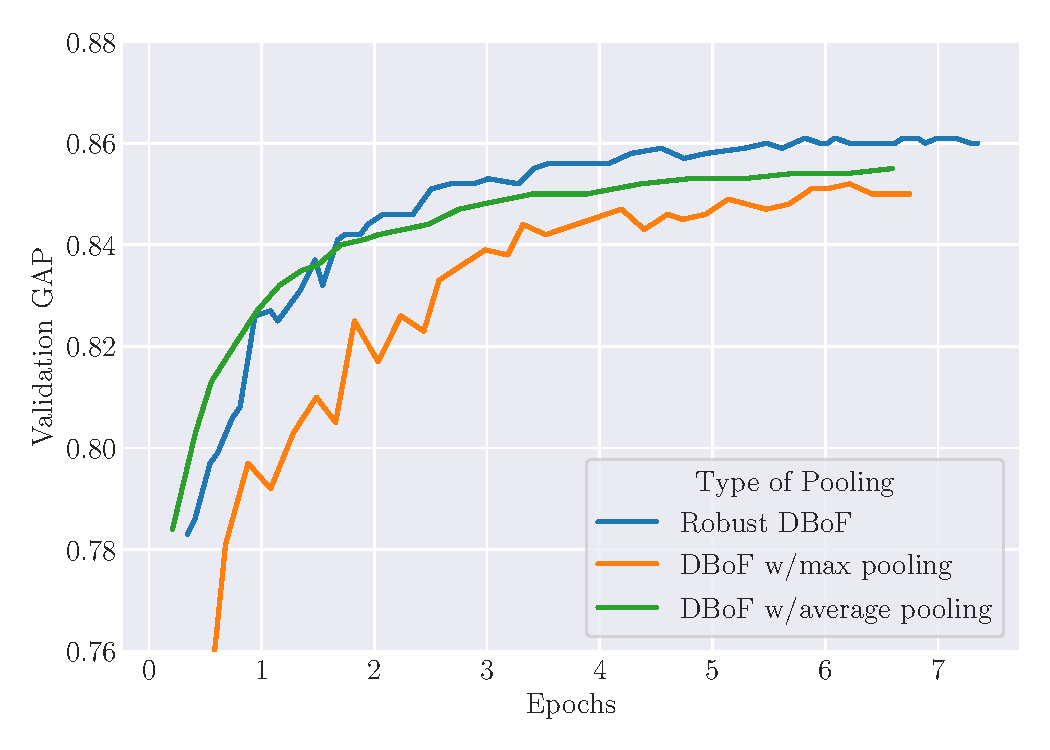
\includegraphics[width=\scalefigure\textwidth]{figures/appendix/ap2-training_video_classification/graph_robust_dbof.pdf}
  \caption{This graphic shows the impact of \emph{robust DBoF} (\ie blue line) with $n=10$ and $k=15$ on the Deep Bag-of-Frames embedding compared to max and average pooling.}
  \label{figure:ap2-learning_curve_bagging}
\end{figure}


\begin{figure}[H]
  \centering
  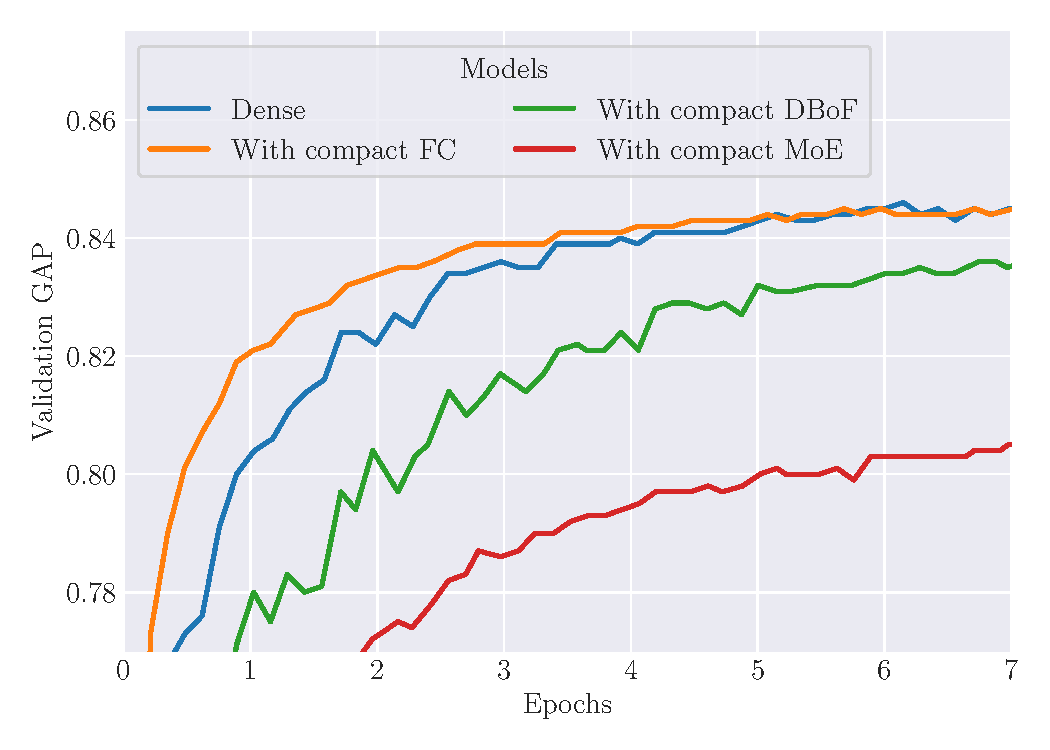
\includegraphics[width=\scalefigure\textwidth]{figures/appendix/ap2-training_video_classification/graph_compact_layers}
  \caption{Validation GAP according to the number of epochs for different compact models.}
  \label{figure:ap2-learning_curve_layers}
	\vspace{1cm}
  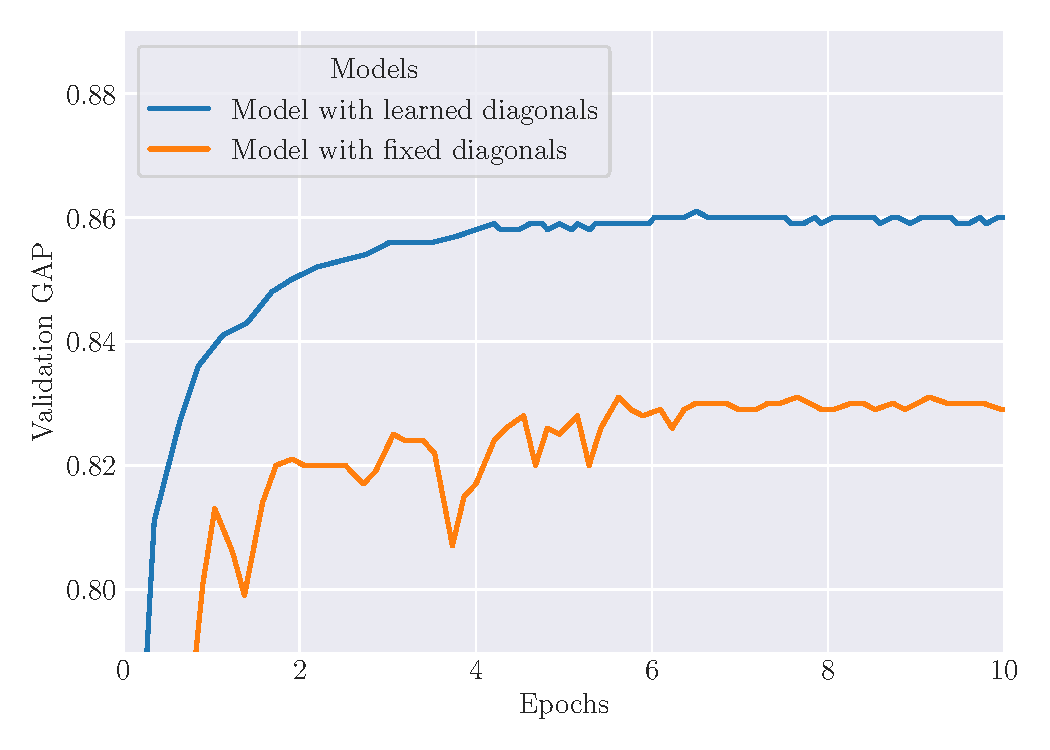
\includegraphics[width=\scalefigure\textwidth]{figures/appendix/ap2-training_video_classification/graph_comparison_learned_diagonal}
	\caption{This figure shows the GAP difference between the approach proposed by~\citet{cheng2015exploration} where the diagonals from the decomposition are initialized from the set $\{-1, +1\}$ and kept fixed and our approach where the values of the diagonals are learned.} 
  \label{figure:ap2-learning_dc_cd}
\end{figure}



\begin{table}[ht]
  \centering
  \begin{tabular}{lccccc}
    \toprule
    \textbf{Model} & \textbf{\#Parameters} & \textbf{CR} & \textbf{GAP@20} & \textbf{Diff.} \\
    \midrule
    % Dense Model  & 45359764 & 173 & - & \textbf{0.846} & -\\
    % Compact DBoF & 36987540 & 141 & 18.4 & 0.838 & -0.008\\
    % Compact FC   & 41181844 & 157 & 9.2 & 0.845 & \textbf{-0.001} \\
    % Compact MoE  & 12668504 & 48 & 72.0 & 0.805 & -0.041 \\
    Dense Model  & 45M &   -- & \textbf{0.846} & -- \\
    Compact DBoF & 36M & 18.4 & 0.838 & -0.008\\
    Compact FC   & 41M &  9.2 & 0.845 & \textbf{-0.001} \\
    Compact MoE  & 12M & 72.0 & 0.805 & -0.041 \\
   \bottomrule
  \end{tabular}
  \caption{This table shows the effect of the compactness of different layers. In these experiments, for speeding-up  the training phase, we did not use the audio features and exploited only the video information.}
  \label{table:ap4-circulant_layer}
\end{table}


%%%%%%%%%%%%%%%%%%%%%%%%%%%%%%%%%%%%%%%%%%%%%%%%%%%%%%%%%%%%%%%%%%%%%%%%%%%%%%%
\subsection{Impact of circulant matrices on different layers}
%%%%%%%%%%%%%%%%%%%%%%%%%%%%%%%%%%%%%%%%%%%%%%%%%%%%%%%%%%%%%%%%%%%%%%%%%%%%%%%

This series of experiments aims at understanding the effect of compactness over different layers.
\Cref{table:ap4-circulant_layer} shows the result in terms of number of weights and GAP.
We also compute the compression ratio (CR) with respect to the dense model.
The compact fully connected layer achieves a compression rate of 9.5 while having a very similar performance, whereas the compact DBoF and MoE achieve a higher compression rate at the expense of accuracy. 
\Cref{figure:ap2-learning_curve_layers} shows that the model with a compact FC converges faster than the dense model.
The model with a compact DBoF shows a big variance over the validation GAP which can be associated with a difficulty to train.
The model with a compact MoE is more stable but at the expense of its performance.

Another series of experiments investigates the effect of adding factors of diagonal circulant layers.
\Cref{table:ap2-factors} shows that there is no gain in accuracy even if the number of weights increases.
It also shows that adding factors has an important effect on the speed of training.
On the basis of this result, \ie given the performance and compression ratio, we can consider that representing the fully connected layer of the base model in a compact fashion can be a good trade-off.


% \begin{figure}[ht]
%   \centering
%   \begin{tikzpicture}[scale=0.7]
\begin{axis}[
    width=0.85\textwidth,
    height=\axisdefaultheight,
    title={\parbox{8cm}{\centering \textbf{Comparison of the effect of compactness over different layers with the base model}}},
    legend columns=2,
    legend style={fill=white,
                  draw=black, 
    			 /tikz/column 2/.style={
                    column sep=5pt,
                  },},
    legend cell align={left},
    xlabel={Epochs},
    ylabel={Validation GAP},
    xmin=0, xmax=7,
    ymin=0.77, ymax=0.87,
    xtick={0,1,2,3,4,5,6,7},
    ytick={0.77,0.78,0.79,0.8,0.81,0.82,0.83,0.84,0.85,0.86,0.87},
    legend pos=north west,
    ymajorgrids=true,
    grid style=dashed,
	]
  \addplot[color=red] table [y=gap, x=epoch]{figures/appendix/ap2-training_video_classification/layers/dense.dat};
  \addplot[color=yellow] table [y=gap, x=epoch]{figures/appendix/ap2-training_video_classification/layers/compact_dbof.dat};
  \addplot[color=blue] table [y=gap, x=epoch]{figures/appendix/ap2-training_video_classification/layers/compact_fc.dat};
  \addplot[color=green] table [y=gap, x=epoch]{figures/appendix/ap2-training_video_classification/layers/compact_moe.dat};
\legend{
   Dense Model,
   Model with compact DBoF, 
   Model with compact FC, 
   Model with compact MoE,
 }
\end{axis}
\end{tikzpicture}

%   \caption{Validation GAP according to the number of epochs for different compact models.}
%   \label{figure:ap2-learning_curve_layers}
% \end{figure}


% \begin{table}[ht]
%   \centering
%   \begin{tabular}{ccccc}
%   \toprule
%   \multirow{2}{*}{\textbf{\#factors}} & \multirow{2}{*}{\textbf{\#Examples/sec}} & \textbf{\#parameters in FC Layer} & \textbf{Compress. Rate of FC layer (\%)} & \multirow{2}{*}{\textbf{GAP@20}} \\
%   \midrule
%   \midrule
%   1 & \numprint{1052} & \numprint{12288} & 99.8 & 0.861 \\
%   3 & 858 & \numprint{73728} & 98.8 & 0.861 \\
%   6 & 568 & \numprint{147456} & 97.6 & 0.859 \\
%   Dense FC & \numprint{1007} & \numprint{6291456} & - & 0.861 \\
%   \bottomrule
%   \end{tabular}
%   \caption{This table shows the evolution of the number of parameters and the accuracy according to the number of factors. Despite the addition of degrees of freedom for the weight matrix of the fully connected layer, the model does not improve in performance. The column \emph{\#Examples/sec} shows the evolution of images per sec processed during the training of the model with a compact FC according to the number of factors.}
%   \label{table:ap2-factors}
% \end{table}

\begin{table}[ht]
  \centering
  \begin{tabular}{ccccc}
    \toprule
    \multirow{2}{*}{\textbf{\#Factors}} & \multicolumn{2}{c}{\textbf{FC Layer}} & \multirow{2}{*}{\textbf{GAP@20}} \\
    \cmidrule{2-3}
     & \textbf{\#Parameters} & \textbf{CR} \\
    \midrule
    -- & 6.29M & -- & 0.861 \\
    1 & 12K & 99.8 & 0.861 \\
    3 & 73K & 98.8 & 0.861 \\
    6 & 147K & 97.6 & 0.859 \\
    \bottomrule
  \end{tabular}
  \caption{This table shows the evolution of the number of parameters and the accuracy according to the number of factors. Despite the addition of degrees of freedom for the weight matrix of the fully connected layer, the model does not improve in performance.}
  \label{table:ap2-factors}
\end{table}


%%%%%%%%%%%%%%%%%%%%%%%%%%%%%%%%%%%%%%%%%%%%%%%%%%%%%%%%%%%%%%%%%%%%%%%%%%%%%%%
\subsection{Comparison with related works}
\label{subsection:ap2-comparison_with_related_works}
%%%%%%%%%%%%%%%%%%%%%%%%%%%%%%%%%%%%%%%%%%%%%%%%%%%%%%%%%%%%%%%%%%%%%%%%%%%%%%%

Circulant matrices have already been used in neural networks by~\cite{cheng2015exploration}.
They proposed to replace fully connected layers by a circulant and diagonal matrices where the circulant matrix is learned by a gradient based optimization algorithm and the diagonal matrix is random with values in \{-1, 1\}.
We compare our more general framework with their approach.
\Cref{figure:ap2-learning_dc_cd} shows the validation GAP according to the number of epochs of the base model with a compact fully connected layer implemented with both approaches.

% \begin{figure}[ht]
%   \centering
%   \begin{tikzpicture}[scale=0.7]
\begin{axis}[
    width=0.85\textwidth,
    height=\axisdefaultheight,
    title={\textbf{GAP given the pooling method used with DBoF embedding}},
    legend style={fill=white,draw=black},
    legend cell align={left},
    xlabel={Epochs},
    ylabel={Validation GAP},
    xmin=0, xmax=10,
    ymin=0.79, ymax=0.88,
    xtick={0,1,2,3,4,5,6,7,8,9,10},
    ytick={0.79,0.80,0.81,0.82,0.83,0.84,0.85,0.86,0.87,0.88},
    legend pos=north west,
    ymajorgrids=true,
    grid style=dashed,
	]
  \addplot[color=red] table [y=gap, x=epoch]{figures/appendix/ap2-training_video_classification/dc_cd/dc.dat};
  \addplot[color=blue] table [y=gap, x=epoch]{figures/appendix/ap2-training_video_classification/dc_cd/cd.dat};
\legend{
 Compact FC w/general approach,
 {Compact FC w/CD and $D \in \{-1, 1\}$},
 }
\end{axis}
\end{tikzpicture}

%   \caption{This figure shows the GAP difference between the $CD$ approach proposed in~\cite{cheng2015exploration} and the more generalized $DC$ approach from~\Cref{subsection:ap2-compact_representation_of_the_base_model}. Instead of having $D \in \{-1, +1\}$ fixed, the generalized approach allows $D$ to be learned.}
%   \label{figure:ap2-learning_dc_cd}
% \end{figure}



%%%%%%%%%%%%%%%%%%%%%%%%%%%%%%%%%%%%%%%%%%%%%%%%%%%%%%%%%%%%%%%%%%%%%%%%%%%%%%%
\subsection{Compact Baseline model with different embeddings}
\label{subsection:ap2-compact_baseline_model_with_different_embeddings}
%%%%%%%%%%%%%%%%%%%%%%%%%%%%%%%%%%%%%%%%%%%%%%%%%%%%%%%%%%%%%%%%%%%%%%%%%%%%%%%

To compare the performance and the compression ratio we can expect, we consider different settings where the compact fully connected layer is used together with different embeddings.
 Figures~\ref{figure:ap2-validation_gap_compact_dbof}, \ref{figure:ap2-validation_gap_compact_netvlad}, \ref{figure:ap2-validation_gap_compact_netfv} and \Cref{table:ap2-fc_circulant_with_diff_embedding} show the performance of the base model with DBoF, NetVLAD and NetFV embeddings with a \emph{Dense} and \emph{Compact} layer.
Notice that we can get a bigger compression rate with NetVLAD and NetFV due to the fact that the output of the embedding is in a higher dimensional space which implies a larger weight matrix for the fully connected layer.
Although the compression rate is higher, it is at the expense of accuracy.



% \begin{figure}[ht]
%   \centering
%   \begin{tikzpicture}[scale=0.56]
\begin{axis}[
    title={\large \textbf{DBoF}},
    legend style={fill=none,draw=none},
    legend cell align={left},
    xlabel={Epochs},
    ylabel={Validation GAP},
    xmin=0, xmax=10,
    ymin=0.81, ymax=0.88,
    xtick={0,1,2,3,4,5,6,7,8,9,10},
    ytick={0.81, 0.82, 0.83,0.84,0.85,0.86, 0.87, 0.88},
    legend pos=north west,
    ymajorgrids=true,
    grid style=dashed,
	]
  \addplot[color=blue] table [y=gap, x=epoch]{figures/appendix/ap2-training_video_classification/fc_circulant_embedding/dbof_compressed.dat};
  \addplot[color=red] table [y=gap, x=epoch]{figures/appendix/ap2-training_video_classification/fc_circulant_embedding/dbof_uncompressed.dat};
\legend{Compact, Dense}
\end{axis}
\end{tikzpicture}
\begin{tikzpicture}[scale=0.56]
\begin{axis}[
    title={\large \textbf{NetVLAD}},
    legend style={fill=none,draw=none},
    legend cell align={left},
    xlabel={Epochs},
    ylabel={Validation GAP},
    xmin=0, xmax=10,
    ymin=0.80, ymax=0.88,
    xtick={0,1,2,3,4,5,6,7,8,9,10},
    ytick={0.81, 0.82, 0.83,0.84,0.85,0.86, 0.87, 0.88},
    legend pos=north west,
    ymajorgrids=true,
    grid style=dashed,
  ]
  \addplot[color=blue] table [y=gap, x=epoch]
  {figures/appendix/ap2-training_video_classification/fc_circulant_embedding/netvlad_compressed.dat};
  \addplot[color=red] table [y=gap, x=epoch]
  {figures/appendix/ap2-training_video_classification/fc_circulant_embedding/netvlad_uncompressed.dat};
\legend{Compact, Dense}
\end{axis}
\end{tikzpicture}
\begin{tikzpicture}[scale=0.56]
\begin{axis}[
    title={\large \textbf{NetFV}},
    legend style={fill=none,draw=none},
    legend cell align={left},
    xlabel={Epochs},
    ylabel={Validation GAP},
    xmin=0, xmax=10,
    ymin=0.810, ymax=0.88,
    xtick={0,1,2,3,4,5,6,7,8,9,10},
    ytick={0.81, 0.82, 0.83, 0.84, 0.85,0.86, 0.87, 0.88},
    legend pos=north west,
    ymajorgrids=true,
    grid style=dashed,
  ]
  \addplot[color=blue] table [y=gap, x=epoch]
  {figures/appendix/ap2-training_video_classification/fc_circulant_embedding/fisher_compressed.dat};
  \addplot[color=red] table [y=gap, x=epoch]
  {figures/appendix/ap2-training_video_classification/fc_circulant_embedding/fisher_uncompressed.dat};
\legend{Compact, Dense}
\end{axis}
\end{tikzpicture}

%   \caption{The figures above show the validation GAP of \textmd{compact} and \emph{Dense} fully connected layer with different embeddings according to the number of epochs.}
%   \label{figure:ap2-learning_curve_circulant}
% \end{figure}


% \begin{table}[ht]
%   \centering
%   \begin{tabular}{lcccc}
%     \toprule
%     \multirow{2}{*}{\textbf{Method}} & \multirow{2}{*}{\textbf{\#Parameters}} & \multirow{2}{*}{\textbf{Size (MB)}} & \textbf{Compress. Rate (\%)} & \multirow{2}{*}{\textbf{GAP@20}} \\
%     \midrule
%     \textbf{DBoF} \\
%     \midrule
% 	\multicolumn{1}{l|}{FC Dense} & \multicolumn{1}{c|}{\numprint{65795732}} & \multicolumn{1}{c|}{251} & \multicolumn{1}{c|}{-} & 0.861 \\
%     \multicolumn{1}{l|}{FC Circulant} & \multicolumn{1}{c|}{\numprint{59528852}} & \multicolumn{1}{c|}{227} & \multicolumn{1}{c|}{9.56} & 0.861 \\
%    \midrule
%    \textbf{NetVLAD} \\
%    \midrule
% 	\multicolumn{1}{l|}{FC Dense} & \multicolumn{1}{c|}{\numprint{86333460}} & \multicolumn{1}{c|}{330} & \multicolumn{1}{c|}{-} & 0.864 \\
%     \multicolumn{1}{l|}{FC Circulant} & \multicolumn{1}{c|}{\numprint{50821140}} & \multicolumn{1}{c|}{194} & \multicolumn{1}{c|}{41.1} & 0.851 \\
%    \midrule
%    \textbf{NetFisher} \\
%    \midrule
% 	\multicolumn{1}{l|}{FC Dense} & \multicolumn{1}{c|}{\numprint{122054676}} & \multicolumn{1}{c|}{466} & \multicolumn{1}{c|}{-} & 0.860 \\
%     \multicolumn{1}{l|}{FC Circulant} & \multicolumn{1}{c|}{\numprint{51030036}} & \multicolumn{1}{c|}{195} & \multicolumn{1}{c|}{58.1} & 0.848 \\
%    \bottomrule
%   \end{tabular}
%   \caption{This table shows the impact of the compression of the fully connected layer of the model architecture shown in~\Cref{figure:ap2-model_baseline} with Audio and Video features vector and different types of embeddings. The variable compression rate is due to the different width of the output of the embedding.}
%   \label{table:ap2-fc_circulant_with_diff_embedding}
% \end{table}


\begin{table}[ht]
  \centering
  \begin{tabular}{llcccc}
    \toprule
    \textbf{Embedding} & \textbf{Method} & \textbf{\#Parameters} & \textbf{CR} & \textbf{GAP@20} \\
    \midrule
    \multirow{2}{*}{\textbf{DBoF}} & FC Dense & 65M & -- & 0.861 \\
     & FC Circulant & 59M & 9.56 & 0.861 \\
    \midrule
    \multirow{2}{*}{\textbf{NetVLAD}} & FC Dense & 86M & -- & 0.864 \\
     &FC Circulant & 50M & 41.1 & 0.851 \\
    \midrule
    \multirow{2}{*}{\textbf{NetFisher}} & FC Dense & 122M & -- & 0.860 \\
     & FC Circulant & 51M & 58.1 & 0.848 \\
    \bottomrule
  \end{tabular}
  \caption{This table shows the impact of the compression of the fully connected layer of the model architecture shown in~\Cref{figure:ap2-model_baseline} with Audio and Video features vector and different types of embeddings. The variable compression rate is due to the different width of the output of the embedding.}
  \label{table:ap2-fc_circulant_with_diff_embedding}
\end{table}





%%%%%%%%%%%%%%%%%%%%%%%%%%%%%%%%%%%%%%%%%%%%%%%%%%%%%%%%%%%%%%%%%%%%%%%%%%%%%%%
\subsection{Tradeoff between Model Size and Accuracy}
\label{subsection:ap2-tradeoff_between_model_size_and_accuracy}
%%%%%%%%%%%%%%%%%%%%%%%%%%%%%%%%%%%%%%%%%%%%%%%%%%%%%%%%%%%%%%%%%%%%%%%%%%%%%%%

% \begin{figure}[ht]
%   \centering
%   \begin{tikzpicture}[scale=0.85]
  \begin{axis}[
%     width=0.6\textwidth,
    height=\axisdefaultheight,
    title={\textbf{Benchmark of compact models}},
    legend style={fill=white,draw=none},
    legend cell align={left},
    xlabel={Number of weights (Millions)},
    ylabel={Validation GAP},
    xmin=0, xmax=200,
    ymin=0.81, ymax=0.88,
    xtick={0, 20, 40,60,80,100,120,140,160,180,200},
    ytick={0.81,0.82,0.83,0.84,0.85,0.86,0.87,0.88},
    legend pos=outer north east,
    ymajorgrids=true,
    grid style=dashed,
  ]
    \addplot[red,    only marks] coordinates {( 25, 0.831)};
    \addplot[orange, only marks] coordinates {( 50, 0.851)};
    \addplot[brown,  only marks] coordinates {( 51, 0.848)};
    \addplot[green,  only marks] coordinates {( 59, 0.861)};
    \addplot[lime,   only marks] coordinates {( 87, 0.858)};
    \addplot[olive,  only marks] coordinates {(158, 0.861)};
    \addplot[blue,   only marks] coordinates {(159, 0.863)};
    \addplot[cyan,   only marks] coordinates {(166, 0.861)};
    \addplot[teal,   only marks] coordinates {(176, 0.861)};
    \legend{
      {NetVLAD 32, Compact FC 256, MoE 2},
      {NetVLAD 64, Compact FC 512, MoE 4},
      {NetFV 64, Compact FC 512, MoE 4},
      {DBoF 8192, Compact FC 512, MoE 4},
      {NetVLAD 256, Compact FC 1024, MoE 4},
      {NetVLAD 128, NetFV 64, Compact FC 1024, MoE 4},
      {NetVLAD 256, NetFV 128, Compact FC 1024, MoE 4},
      {DBoF 8192,  NetVLAD 128, Compact FC 1024, MoE 4},
      {DBoF 16384, NetVLAD 256, Compact FC 1024, MoE 4},
    }
  \end{axis}
\end{tikzpicture}
%   \caption{Comparison between different models with compact fully connected layers.}
%   \label{figure:ap2-models}
% \end{figure}

To conclude our experimental evaluation, we compare all our models in terms of size and accuracy.
The results are presented in~\Cref{figure:ap2-models}. 
As we can see in this figure, the most compact models are obtained with the circulant NetVLAD and NetFV.
We can also see that the complex architectures described in~\Cref{subsection:ap2-leveraging_architectural_diversity} (DBoF + NetVLAD) achieve top performance but at the cost of a large number of weights.
Finally, the best trade-off between size and accuracy is obtained using the DBoF embedding layer and achieves a GAP of 0.861 for only 60 millions weights.


%%%%%%%%%%%%%%%%%%%%%%%%%%%%%%%%%%%%%%%%%%%%%%%%%%%%%%%%%%%%%%%%%%%%%%%%%%%%%%%
\section{Conclusion}
\label{section:ap2-conclusion}
%%%%%%%%%%%%%%%%%%%%%%%%%%%%%%%%%%%%%%%%%%%%%%%%%%%%%%%%%%%%%%%%%%%%%%%%%%%%%%%

In this appendix, we demonstrated that circulant matrices and diagonal matrices can be a great tool to design compact neural network architectures for video classification tasks.
Our experiments demonstrate that the best trade-off between size and accuracy is obtained using circulant DBoF embedding layers.
We investigated a model with multiple embeddings to leverage the performance of an Ensemble but found it ineffective.
The good performance of Ensemble models, \ie, why aggregating different distinct models performs better that incorporating all the diversity in a single architecture is still an open problem.
Our future work will be devoted to address this challenging question and to pursue our effort to devise compact models achieving the same accuracy as larger one, and to study their theoretical properties.

\newpage


\begin{figure}[H]
	\center
	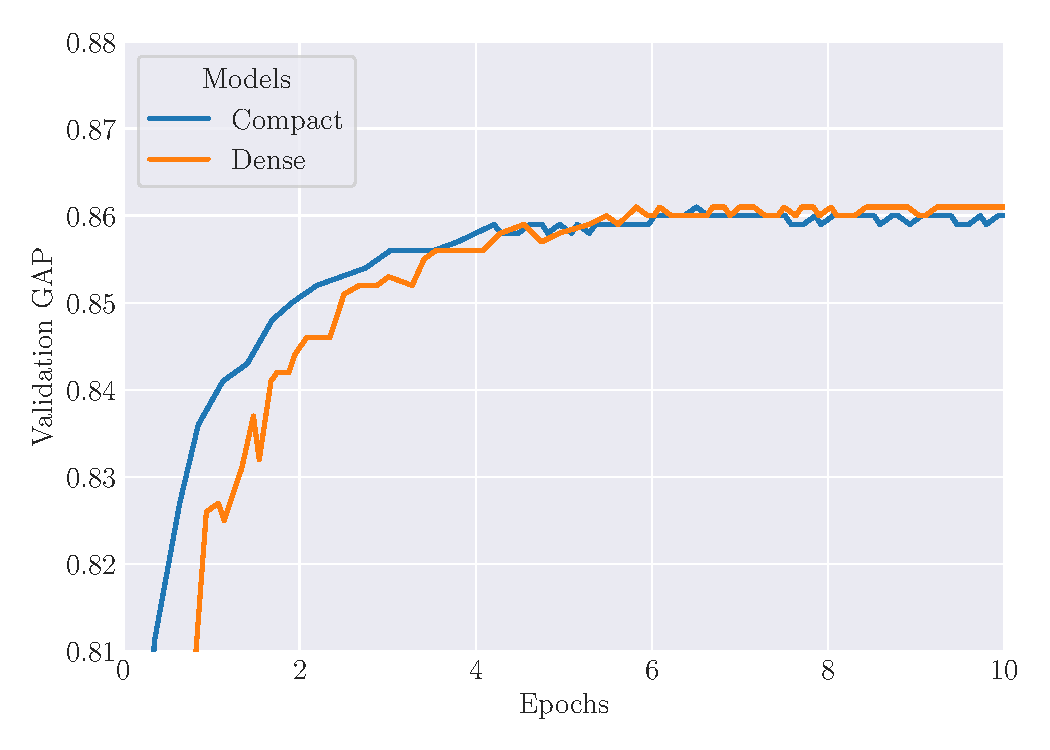
\includegraphics[width=\scalefigure\textwidth]{figures/appendix/ap2-training_video_classification/graph_fc_circulant_embedding_dbof}
	\caption{Validation GAP of compact DBoF embedding and dense fully connected layer.}
	\label{figure:ap2-validation_gap_compact_dbof}
	\vspace{1cm}
	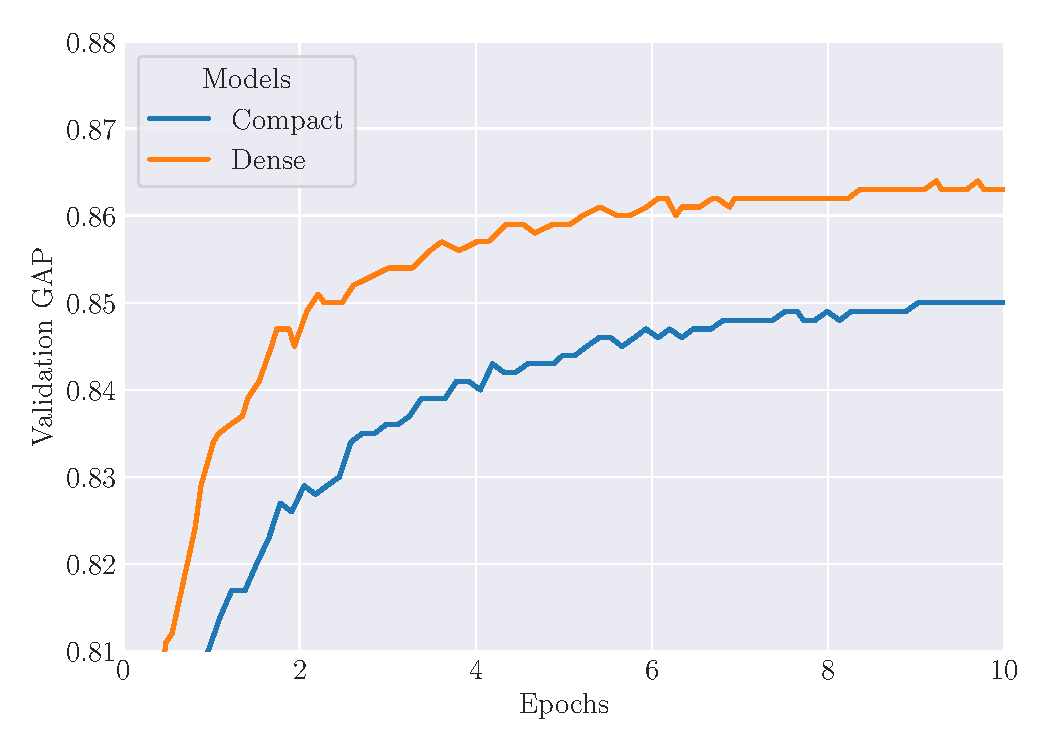
\includegraphics[width=\scalefigure\textwidth]{figures/appendix/ap2-training_video_classification/graph_fc_circulant_embedding_netvlad}
	\caption{Validation GAP of compact NetVLAD embedding and dense fully connected layer.}
	\label{figure:ap2-validation_gap_compact_netvlad}
\end{figure}

\begin{figure}[H]
	\center
	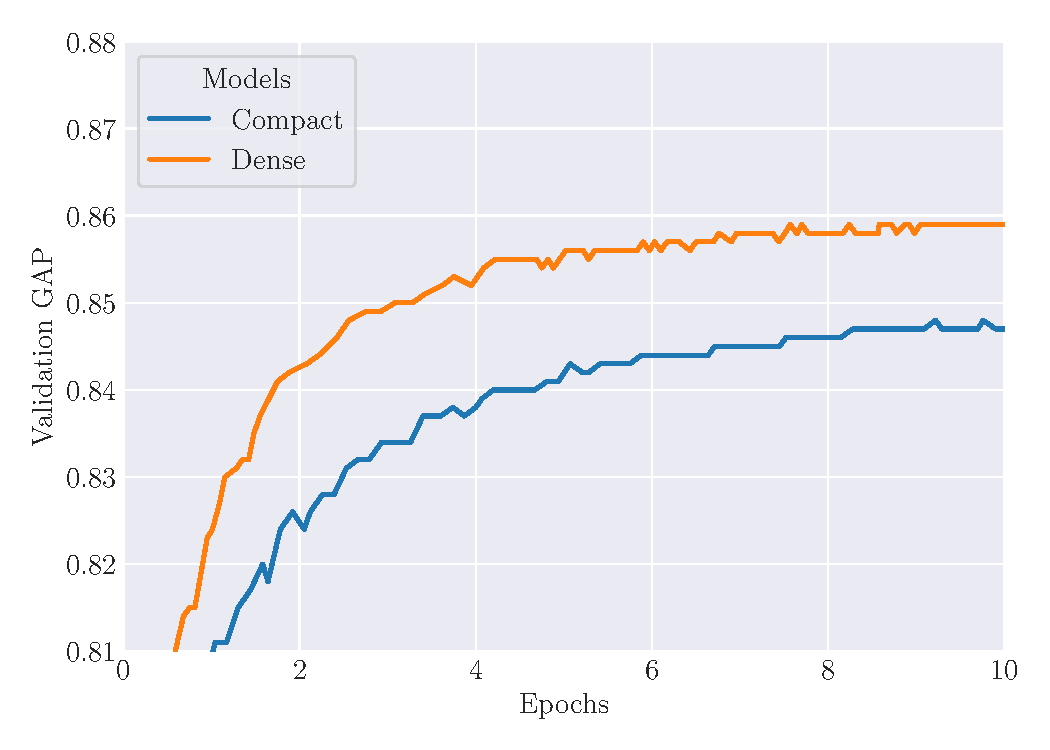
\includegraphics[width=\scalefigure\textwidth]{figures/appendix/ap2-training_video_classification/graph_fc_circulant_embedding_netfv}
	\caption{Validation GAP of compact NetFV embedding and dense fully connected layer.}
	\label{figure:ap2-validation_gap_compact_netfv}
	\vspace{1cm}
	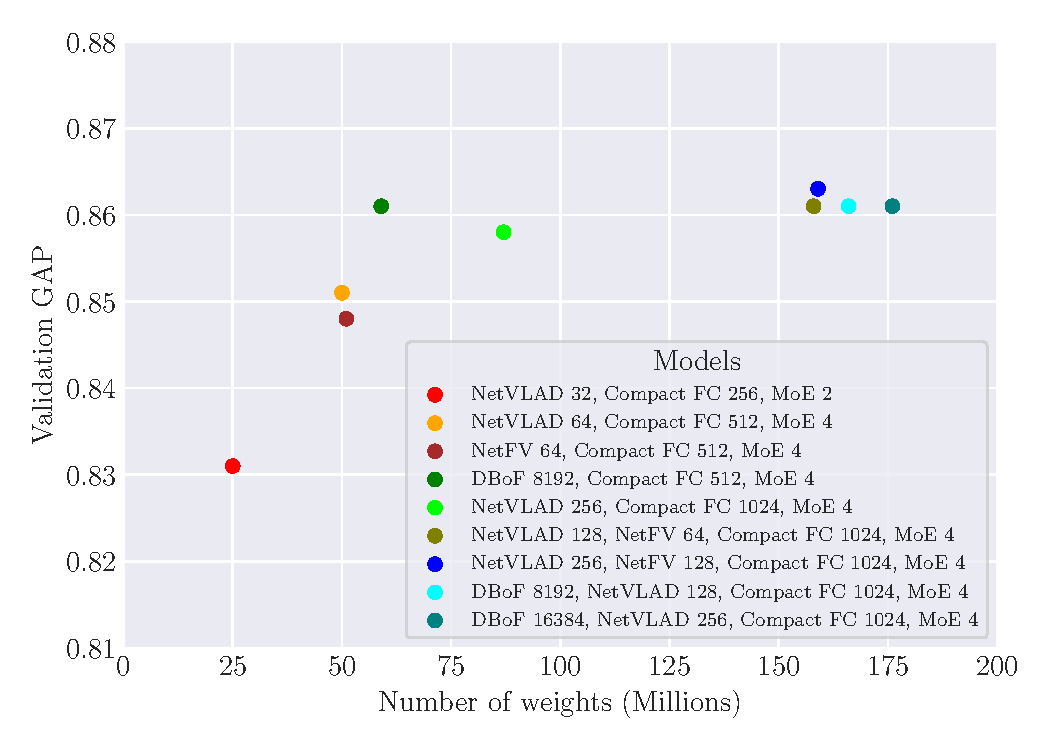
\includegraphics[width=\scalefigure\textwidth]{figures/appendix/ap2-training_video_classification/graph_benchmark_models}
	\caption{Comparison between different models with compact fully connected layers.}
	\label{figure:ap2-models}
\end{figure}





  %   %%%%%%%%%%%%%%%%%%%%%%%%%%%%%%%%%%%%%%%%%%%%%%%%%%%%%%%%%%%%%%%%%%%%%%%%%%%%%%%
\chapter{Theoretical Evidence for Adversarial Robustness through Randomization}
\label{appendix:ap3-theoretical_evidence_for_adversarial_robustness_through_randomization}
%%%%%%%%%%%%%%%%%%%%%%%%%%%%%%%%%%%%%%%%%%%%%%%%%%%%%%%%%%%%%%%%%%%%%%%%%%%%%%%
\localtoc

\vspace{\fill}

\noindent
\emph{
This Appendix concerns a collaboration with Rafael Pinot, Laurent Meunier, Hisashi Kashima, Florian Yger, Cédric Gouy-Pailler and Jamal Atif.
This work has been published at the Conference on Neural Information Processing Systems (NeurIPS) 2019.
It investigates the theory of robustness against adversarial attacks. It focuses on the family of randomization techniques that consist in injecting noise in the network at inference time.
All proofs of this appendix can be found in the long version of the paper.\footnote{https://arxiv.org/abs/1902.01148}
For simplification, we left the notation as in the original paper.
}

\vspace{\fill}

% \begin{abstract}
%     This paper investigates the theory of robustness against adversarial attacks. It focuses on the family of randomization techniques that consist in injecting noise in the network at inference time. These techniques have proven effective in many contexts, but lack theoretical arguments. We close this gap by presenting a theoretical analysis of these approaches, hence explaining why they perform well in practice. More precisely, we make two  new contributions. The first one relates the randomization rate to robustness to adversarial attacks. This result applies for the general family of exponential distributions, and thus extends and unifies the previous approaches. The second contribution consists in devising a new upper bound on the adversarial generalization gap of randomized neural networks. We support our theoretical claims with a set of experiments.
% \end{abstract}


%%%%%%%%%%%%%%%%%%%%%%%%%%%%%%%%%%%%%%%%%%%%%%%%%%%%%%%%%%%%%%%%%%%%%%%%%%%%%%%
\section{Introduction}
\label{section:ap3-introduction}
%%%%%%%%%%%%%%%%%%%%%%%%%%%%%%%%%%%%%%%%%%%%%%%%%%%%%%%%%%%%%%%%%%%%%%%%%%%%%%%

Adversarial attacks are some of the most puzzling and burning issues in modern machine learning.
An adversarial attack refers to a small, imperceptible change of an input maliciously designed to fool the result of a machine learning algorithm.
Since the seminal work of~\citet{szegedy2013intriguing} exhibiting this intriguing phenomenon in the context of deep learning, a wealth of results have been published on designing attacks~\cite{goodfellow2014explaining,papernot2016limitations,moosavi2016deepfool,kurakin2016adversarial,carlini2017towards,moosavi2017universal} and defenses~\cite{goodfellow2014explaining,papernot2016distillation,guo2017countering,meng2017magnet,samangouei2018defense,madry2018towards}), or on trying to understand the very nature of this phenomenon~\cite{fawzi2018empirical,simon2018adversarial,fawzi2018adversarial,moosavi2016robustness}.
Most methods remain unsuccessful to defend against powerful adversaries~\cite{carlini2017towards,madry2018towards,athalye2018obfuscated}.
Among the defense strategies, randomization has proven effective in some contexts.
It consists in injecting random noise (both during training and inference phases) inside the network architecture, \ie, at a given layer of the network.
Noise can be drawn either from Gaussian~\cite{xuanqing2018towards,lecuyer2018certified,rakin2018parametric}, Laplace~\cite{lecuyer2018certified}, Uniform~\cite{xie2017mitigating}, or Multinomial~\cite{dhillon2018stochastic} distributions.
Remarkably, most of the considered distributions belong to the Exponential family.
Albeit these significant efforts, several theoretical questions remain unanswered.
Among these, we tackle the following, for which we provide principled and theoretically-founded answers:
\begin{itemize}
    \item[\textbf{Q1:}] To what extent does a noise drawn from the Exponential family preserve robustness (in a sense to be defined) to adversarial attacks?
\end{itemize}

\paragraph{A1:}
We introduce a definition of robustness to adversarial attacks that is suitable to the randomization defense mechanism.
As this mechanism can be  described as a non-deterministic querying process, called probabilistic mapping in the sequel, we propose a formal definition of robustness relying on a metric/divergence between probability measures.
A key question arises then about the appropriate metric/divergence for our context.
This requires tools for comparing divergences \wrt the introduced robustness definition.
Renyi divergence turned out to be a measure of choice, since it satisfies most of the desired properties  (coherence, strength, and computational tractability).
Finally, thanks to the existing links between the Renyi divergence and the Exponential family, we were able to prove  that methods based on noise injection from the Exponential family  ensures robustness to adversarial examples (cf. \Cref{theorem:ap3-netrob}).
\begin{itemize}
    \item[\textbf{Q2:}] Can we guarantee a good accuracy under attack for classifiers defended with this kind of noise? 
\end{itemize}

\paragraph{A2:}
We present an upper bound on  the drop of accuracy (under attack) of the methods defended with noise drawn from the Exponential family (cf. \Cref{theorem:ap3-bound}).
Then, we illustrate this result by training different randomized models with Laplace and Gaussian distributions on CIFAR10/CIFAR100.
These experiments highlight the trade-off between accuracy and robustness that depends on the amount of noise one injects in the network.
Our theoretical and experimental conclusion is that randomized defenses are competitive (with the current state-of-the-art~\cite{madry2018towards}) given the intensity of noise injected in the network.

\paragraph{Outline of the chapter:}
We present in \Cref{section:ap3-relatedwork} the related work on randomized defenses to adversarial examples.
\Cref{section:ap3-definition} introduces the definition of robustness relying on a metric/divergence between probability measures, and discusses the key role of the Renyi divergence.
We state in~\Cref{sec:main_result} our main results on the robustness and accuracy of Exponential family-based defenses.
\Cref{section:ap3-experiment} presents extensive experiments supporting our theoretical findings.
\Cref{section:ap3-conclusion_remarks} provides concluding remarks.

%%%%%%%%%%%%%%%%%%%%%%%%%%%%%%%%%%%%%%%%%%%%%%%%%%%%%%%%%%%%%%%%%%%%%%%%%%%%%%%
\section{Related works}
\label{section:ap3-relatedwork}
%%%%%%%%%%%%%%%%%%%%%%%%%%%%%%%%%%%%%%%%%%%%%%%%%%%%%%%%%%%%%%%%%%%%%%%%%%%%%%%

Injecting noise into algorithms to improve their robustness has been used for ages in detection and signal processing tasks~\cite{zozor1999stochastic,chapeau2004noise,mitaim1998adaptive}.
It has also been extensively studied in several machine learning and optimization fields, \eg robust optimization~\cite{ben2009robust} and data augmentation techniques~\cite{perez2017effectiveness}.
Recently, noise injection techniques have been adopted by the adversarial defense community, especially for neural networks, with very promising results.
Randomization techniques are generally oriented towards one of the following objectives: experimental robustness or provable robustness.

\paragraph{Experimental robustness:}
The first technique explicitly using randomization at inference time as a defense appeared during the 2017 NeurIPS defense challenge~\cite{xie2017mitigating}.
This method uniformly samples over geometric transformations of the image to select a substitute image to feed the network.
Then~\citet{dhillon2018stochastic} proposed to use stochastic activation pruning based on a multinomial distribution for adversarial defense.
Several works~\cite{xuanqing2018towards,rakin2018parametric} propose to inject Gaussian noise directly on the activation of selected layers both at training and inference time.
While these works hypothesize that noise injection makes the network robust to adversarial perturbations, they do not provide any formal justification on the nature of the noise they use or on the loss of accuracy/robustness of the  network.

\paragraph{Provable robustness:}
\citet{lecuyer2018certified} proposed a randomization method by exploiting the link between differential privacy~\cite{dwork2014algorithmic} and adversarial robustness.
Their framework, called ``randomized smoothing'' \footnote{Name introduced by~\citet{cohen2019certified} after the work of~\cite{lecuyer2018certified}.}, inherits some theoretical results from the differential privacy community allowing them to evaluate the level of accuracy under attack of their method.
Initial results by~\citet{lecuyer2018certified} have been refined by~\citet{li2018second}, and by~\citet{cohen2019certified}.
Our work belongs to this line of research.
However, our framework does not treat exactly the same class of defenses.
Notably, we provide theoretical arguments supporting the defense strategy based on randomization techniques relying on the exponential family, and derive a new bound on the adversarial generalization gap, which completes the results obtained so far on certified robustness.
Furthermore, our focus is on the network randomized by noise injection, ``randomized smoothing'' instead uses this network to create a \emph{new} classifier robust to attacks.

Since the initial discovery of adversarial examples, a wealth of non randomized defense approaches have also been proposed, inspired by various machine learning domains such as adversarial training~\cite{goodfellow2014explaining,madry2018towards}, image reconstruction~\cite{meng2017magnet,samangouei2018defense} or robust learning~\cite{goodfellow2014explaining,madry2018towards}.
Even if these methods have their own merits, a thorough evaluation made by~\citet{athalye2018obfuscated} shows that most defenses can be easily broken with known powerful attacks~\cite{madry2018towards,carlini2017towards,chen2018ead}.
Adversarial training, which consists in training a model directly on adversarial examples, came out as the best defense in average.
Defense based on randomization could be overcome by the Expectation Over Transformation technique proposed by~\citet{athalye2017synthesizing} which consists in taking the expectation over the network to craft the perturbation.
In this chapter, to ensure that our results are not biased by obfuscated gradients, we follow the principles provided by~\cite{athalye2018obfuscated,carlini2019evaluating} and evaluate our randomized networks with this technique.
We show that randomized defenses are still competitive given the intensity of noise injected in the network.

%%%%%%%%%%%%%%%%%%%%%%%%%%%%%%%%%%%%%%%%%%%%%%%%%%%%%%%%%%%%%%%%%%%%%%%%%%%%%%%
\section{General definitions of risk and robustness}
\label{section:ap3-definition}
%%%%%%%%%%%%%%%%%%%%%%%%%%%%%%%%%%%%%%%%%%%%%%%%%%%%%%%%%%%%%%%%%%%%%%%%%%%%%%%

%%%%%%%%%%%%%%%%%%%%%%%%%%%%%%%%%%%%%%%%%%%%%%%%%%%%%%%%%%%%%%%%%%%%%%%%%%%%%%%
\subsection{Risk, robustness and probabilistic mappings}
%%%%%%%%%%%%%%%%%%%%%%%%%%%%%%%%%%%%%%%%%%%%%%%%%%%%%%%%%%%%%%%%%%%%%%%%%%%%%%%

Let us consider two spaces $\mathcal{X}$ (with norm $\norm{\ \cdot\ }_{\mathcal{X}}$), and $\mathcal{Y}$.
We consider the classification task that seeks a hypothesis (classifier) $h: \mathcal{X} \rightarrow \mathcal{Y}$ minimizing the risk of $h$ \wrt some ground-truth distribution $\mathcal{D}$ over $\mathcal{X}\times\mathcal{Y}$.
The risk of $h$ \wrt $\mathcal{D}$ is defined as 
\begin{align*}
  \Risk(h) \triangleq \mathbb{E}_{(x,y)\sim \mathcal{D}}\left[ \mathds{1} \left( h(x) \neq y \right)\right].
\end{align*}
Given a classifier $h: \mathcal{X} \rightarrow \mathcal{Y}$, and some input $x \in \mathcal{X}$ with true label $y_{true} \in \mathcal{Y}$, to generate an adversarial example, the adversary seeks a $\tau$ such that $h(x+\tau) \neq y_{true}$, with some budget $\alpha$ over the perturbation (\ie, with $\norm{\tau}_{\mathcal{X}} \leq\alpha$).
$\alpha$ represents the maximum amount of perturbation one can add to $x$ without being spotted (the perturbation remains humanly imperceptible). 
The overall goal of the adversary is to find a perturbation crafting strategy that both maximizes the risk of $h$, and keeps the values of $\norm{\tau}_{\mathcal{X}}$ small.
To measure this risk "under attack" we define the notion of adversarial $\alpha$-radius risk of $h$ \wrt $\mathcal{D}$ as follows
\begin{align}
    \advRisk(h) \triangleq \mathbb{E}_{(x,y) \sim \mathcal{D}} \left[ \sup_{\norm{\tau}_{\mathcal{X}} \leq \alpha} \mathds{1}\left(h(x+\tau) \neq y\right) \right]\enspace.
\end{align}

In practice, the adversary does not have any access to the ground-truth distribution.
The literature proposed several surrogate versions of $\advRisk(h)$ (see~\citet{diochnos2018adversarial} for more details) to overcome this issue.
We focus our analysis on the one used by~\citet{szegedy2013intriguing,fawzi2018adversarial} denoted $\alpha$-radius prediction-change risk of $h$ \wrt $\mathcal{D}_{\mathcal{X}}$ (marginal of $\mathcal{D}$ for $\mathcal{X}$), and defined as   
\begin{align}
    \PCadvRisk(h) \triangleq \mathbb{P}_{x\sim \mathcal{D}_{\mathcal{X}}}\left[\exists \tau \in \B \text{ s.t. } h(x+\tau)\neq h(x) \right]
\end{align}
where for any $\alpha \geq 0$, \quad $\B \triangleq \{\tau \in \mathcal{X} \text{ s.t. } \norm{\tau}_{\mathcal{X}} \leq \alpha\}\enspace.$

As we will inject some noise in our classifier in order to defend against adversarial attacks, we need to introduce the notion of ``probabilistic mapping''. Let $\mathcal{Y}$ be the output space, and $\mathcal{F}_{\mathcal{Y}}$ a $\sigma$-$ algebra$ over $\mathcal{Y}$. Let us also denote $\mathcal{P}(\mathcal{Y})$ the set of probability measures over $(\mathcal{Y},\mathcal{F}_{\mathcal{Y}})$.

\begin{definition}[Probabilistic mapping] Let $\mathcal{X}$ be an arbitrary space, and $(\mathcal{Y},\mathcal{F}_{\mathcal{Y}})$ a measurable space. A \emph{probabilistic mapping} from $\mathcal{X}$ to $\mathcal{Y}$ is a mapping $\probmap: \mathcal{X} \to \mathcal{P}(\mathcal{Y})$.
To obtain a numerical output out of this \emph{probabilistic mapping}, one needs to sample $y$ according to $\probmap(x)$. %$y\sim \probmap(x)$.
\end{definition} 

This definition does not depend on the nature of $\mathcal{Y}$ as long as $(\mathcal{Y},\mathcal{F}_{\mathcal{Y}})$ is measurable.
In that sense, $\mathcal{Y}$ could be either the label space or any intermediate space corresponding to the output of an arbitrary hidden layer of a neural network.
Moreover, any mapping can be considered as a probabilistic mapping, whether it explicitly injects noise (see~\citet{lecuyer2018certified,rakin2018parametric,dhillon2018stochastic}) or not.
In fact, any deterministic mapping can be considered as a probabilistic mapping, since it can be characterized by a Dirac measure.
Accordingly, the definition of a probabilistic mapping is fully general and equally treats networks with or without noise injection.
There exists no definition of robustness against adversarial attacks that comply with the notion of probabilistic mappings.
We settle that by generalizing the notion of prediction-change risk initially introduced by~\citet{diochnos2018adversarial} for deterministic classifiers.
Let $\probmap$ be a probabilistic mapping from $\mathcal{X}$ to $\mathcal{Y}$, and $d_{\mathcal{P}(\mathcal{Y})}$ some metric/divergence on $\mathcal{P}(\mathcal{Y})$.
We define the $(\alpha,\epsilon)$-radius prediction-change risk of $\probmap$ \wrt $\mathcal{D}_{\mathcal{X}}$ and $d_{\mathcal{P}(\mathcal{Y})}$ as 
\begin{equation}
  \PCadvRisk(\probmap,\epsilon) \triangleq  \mathbb{P}_{x\sim \mathcal{D}_{\mathcal{X}}}\left[ \exists \tau \in B(\alpha) \text{ s.t. } d_{\mathcal{P}(\mathcal{Y})}(\probmap(x+\tau),\probmap(x)) > \epsilon \right] \enspace.
\end{equation}

\noindent
These three generalized notions allow us to analyze noise injection defense mechanisms (Theorems~\ref{theorem:ap3-netrob}, and~\ref{theorem:ap3-bound}).
We can also define adversarial robustness (and later adversarial gap) thanks to these notions. 
\begin{definition}[Adversarial robustness] \label{def::GeneralizedRobustness}
  Let $d_{\mathcal{P}(\mathcal{Y})}$ be a metric/divergence on $\mathcal{P}(\mathcal{Y})$.
  The probabilistic mapping $\probmap$ is said to be $d_{\mathcal{P}(\mathcal{Y})}$-$(\alpha, \epsilon, \gamma)$ robust if 
  \begin{equation}
    \PCadvRisk(\probmap,\epsilon) \leq \gamma \enspace.
  \end{equation}
  \removespace
\end{definition}

\noindent
It is difficult in general to show that a classifier is $d_{\mathcal{P}(\mathcal{Y})}$-$(\alpha, \epsilon, \gamma)$ robust.
However, we can  derive some bounds for particular divergences that will ensure robustness up to a certain level (Theorem~\ref{theorem:ap3-netrob}).
It is worth noting that our definition of robustness depends on the considered metric/divergence between probability measures.
Lemma~\ref{th::PropimpliesRobustness} gives some insights on the monotony of the robustness according to the parameters, and the probability metric/divergence at hand.

\begin{lemma} \label{th::PropimpliesRobustness}
  Let $\probmap$ be a probabilistic mapping, and let  $d_{1}$ and $d_{2}$ be two metrics on $\mathcal{P}(\mathcal{Y})$.
  If there exists a non decreasing function $ \phi: \mathbb{R} \to \mathbb{R}$ such that $\forall \mu_1,\mu_2 \in \mathcal{P}(\mathcal{Y})$, $d_{1}(\mu_1,\mu_2) \leq \phi(d_{2}(\mu_1,\mu_2)) $, then the following assertion holds: 
  \begin{equation}
    \probmap \text{ is } d_{2}\text{-}(\alpha, \epsilon, \gamma)\text{-robust} \implies \probmap \text{ is }d_{1}\text{-}(\alpha, \phi(\epsilon), \gamma)\text{-robust}
  \end{equation}
  \removespace
\end{lemma}
\noindent
As suggested in Definition~\ref{def::GeneralizedRobustness} and Lemma~\ref{th::PropimpliesRobustness}, any given choice of metric/divergence will instantiate a particular notion of adversarial robustness and it should be carefully selected. 

%%%%%%%%%%%%%%%%%%%%%%%%%%%%%%%%%%%%%%%%%%%%%%%%%%%%%%%%%%%%%%%%%%%%%%%%%%%%%%%%
\subsection{On the choice of the metric/divergence for robustness}
\label{subsec:div}
%%%%%%%%%%%%%%%%%%%%%%%%%%%%%%%%%%%%%%%%%%%%%%%%%%%%%%%%%%%%%%%%%%%%%%%%%%%%%%%%

The aforementioned formulation naturally raises the question of the choice of the metric used to defend against adversarial attacks. 
The main notions that govern the selection of an appropriate metric/divergence are  \emph{coherence}, \emph{strength}, and \emph{computational tractability}.
A metric/divergence is said to be coherent if it naturally fits the task at hand (\eg classification tasks are intrinsically linked to discrete/trivial metrics, conversely to regression tasks).
The strength of a metric/divergence refers to its ability to cover (dominate) a wide class of others in the sense of Lemma~\ref{th::PropimpliesRobustness}. 
In the following, we will focus on both the total variation metric and the Renyi divergence, that we consider as respectively the most coherent with the classification task using probabilistic mappings, and the strongest divergence.
We first discuss how total variation metric is \emph{coherent} with randomized classifiers but suffers from computational issues.
Hopefully, the Renyi divergence provides good guarantees about adversarial robustness, enjoys nice \emph{computational properties}, in particular when considering  Exponential family distributions, and is \emph{strong} enough to dominate a wide range of metrics/divergences including total variation.


Let  $\mu_1$ and $\mu_2$ be two measures in $\mathcal{P}(\mathcal{Y})$, both dominated by a third measure $\nu$.
The trivial distance $ d_{T}(\mu_1,\mu_ \triangleq \mathds{1}\left(\mu_1 \neq \mu_2\right)$ is the simplest distance one can define between $\mu_1$ and $\mu_2$.
In the deterministic case, it is straightforward to compute (since the numerical output of the algorithm characterizes its associated measure), but this is not the case in general.
In fact one might not have access to the true distribution of the mapping, but just to the numerical outputs.
Therefore, one needs to consider more sophisticated metrics/divergences, such as the total variation distance $d_{TV}(\mu_1,\mu_2) \triangleq \sup_{Y \in \mathcal{F}_{\mathcal{Y}}} |\mu_1 (Y) - \mu_2(Y)|$.
The total variation distance is one of the most broadly used probability metrics.
It admits several very simple interpretations, and is a very useful tool in many mathematical fields such as probability theory, Bayesian statistics, coupling or transportation theory.
In transportation theory, it can be rewritten as the solution of the Monge-Kantorovich problem with the cost function $c(y_1,y_2) =\mathds{1}\left(y_1 \neq y_2\right)$: $ \inf\int_{\mathcal{Y}^{2}}\mathds{1}\left(y_1 \neq y_2\right) d\pi(y_1,y_2)\, ,$ where the infimum is taken over all joint probability measures $\pi$ on $(\mathcal{Y}\times \mathcal{Y}, \mathcal{F}_{\mathcal{Y} } \otimes \mathcal{F}_{\mathcal{Y}})$ with marginals $\mu_1$ and $\mu_2$.
According to this interpretation, it seems quite natural to consider the total variation distance as a relaxation of the trivial distance on $[0,1]$ (see the book of~\citet{villani2008optimal} for details).
In the deterministic case, the total variation and the trivial distance coincides.
In general, the total variation allows a finer analysis of the probabilistic mappings than the trivial distance.
But it suffers from a high computational complexity.
In the following of the chapter we will show how to ensure robustness regarding TV distance.

Finally, denoting by $g_1$ and $g_2$ the respective probability distributions \wrt $\nu$, the Renyi divergence of order $\lambda$~\cite{renyi1961} writes as  
\begin{equation}
  d_{R,\lambda}(\mu_1,\mu_2) \triangleq \frac{1}{\lambda -1}\log \int_{\mathcal{Y}} g_2(y)  \left(\frac{g_1(y)}{g_2(y)}\right)^{\lambda} d\nu(y).
\end{equation}
The Renyi divergence is a generalized measure defined on the interval $(1,\infty)$, where it equals the Kullback-Leibler divergence when $\lambda \rightarrow 1$ (that will be denoted $d_{KL}$), and the maximum divergence when $\lambda \rightarrow \infty$.
It also has the very special property of being non decreasing \wrt $\lambda$.
This divergence is very common in machine learning, especially in its Kullback-Leibler form as it is widely used as the loss function (cross entropy) of classification algorithms.
It enjoys the desired properties  since it bounds the TV distance, and is tractable.
Furthermore, Proposition~\ref{proposition:ap3-RobustTV} proves that Renyi-robustness implies TV-robustness, making it a suitable surrogate for the trivial distance.

\begin{proposition}[Renyi-robustness implies TV-robustness] \label{proposition:ap3-RobustTV}
  Let $\probmap$ be a probabilistic mapping, then $\forall\lambda\geq1$:
  \begin{equation}
    \probmap \text{ is }  d_{R,\lambda}\text{-}(\alpha, \epsilon, \gamma)\text{-robust} \implies \probmap \text{ is } d_{TV}\text{-}(\alpha, \epsilon', \gamma)\text{-robust}
  \end{equation}
  \begin{equation}
    \textnormal{ with } \epsilon' = \min \left(\frac{3}{2}\left(\sqrt{1 + \frac{4\epsilon}{9}} - 1\right)^{1/2}, \frac{\exp(\epsilon +1) -1}{\exp(\epsilon +1) +1}\right) \enspace.
  \end{equation}
  \removespace
\end{proposition}

\noindent
A crucial property of Renyi-robustness is the \textit{Data processing inequality}.
It is a well-known inequality from information theory which states that \textit{``post-processing cannot increase information''}~\cite{cover2012elements,beaudry2011intuitive}.
In our case, if we consider a Renyi-robust probabilistic mapping, composing it with a deterministic mapping maintains Renyi-robustness with the same level.

\begin{proposition}[Data processing inequality] \label{proposition:ap3-postprocessing}
  Let us consider a probabilistic mapping $\probmap:\mathcal{X}\rightarrow\mathcal{P}(\mathcal{Y})$. Let us also denote $\rho:\mathcal{Y}\rightarrow\mathcal{Y}'$ a deterministic function.
  If $U \sim \probmap(x)$ then the probability measure $M'(x)$ s.t $\rho(U) \sim M'(x)$ defines a probabilistic mapping $M':\mathcal{X}\rightarrow\mathcal{P}(\mathcal{Y}')$.
  For any $\lambda>1$ if $\probmap$ is $d_{R,\lambda}$-$(\alpha,\epsilon,\gamma)$ robust then $M'$ is also is $d_{R,\lambda}$-$(\alpha,\epsilon,\gamma)$ robust.
\end{proposition}
\noindent
Data processing inequality will allow us later to inject some additive noise in any layer of a neural network and to ensure Renyi-robustness.

%%%%%%%%%%%%%%%%%%%%%%%%%%%%%%%%%%%%%%%%%%%%%%%%%%%%%%%%%%%%%%%%%%%%%%%%%%%%%%%
\section{Defense mechanisms based on  Exponential family noise injection}
\label{sec:main_result}
%%%%%%%%%%%%%%%%%%%%%%%%%%%%%%%%%%%%%%%%%%%%%%%%%%%%%%%%%%%%%%%%%%%%%%%%%%%%%%%

%%%%%%%%%%%%%%%%%%%%%%%%%%%%%%%%%%%%%%%%%%%%%%%%%%%%%%%%%%%%%%%%%%%%%%%%%%%%%%%
\subsection{Robustness through Exponential family noise injection}
%%%%%%%%%%%%%%%%%%%%%%%%%%%%%%%%%%%%%%%%%%%%%%%%%%%%%%%%%%%%%%%%%%%%%%%%%%%%%%%

For now, the question of which class of noise to add is treated \textit{ad hoc}.
We choose here to investigate one particular class of noise closely linked to the Renyi divergence, namely Exponential family distributions, and demonstrate their interest.
Let us first recall what the Exponential family is.

\begin{definition}[Exponential family]
  Let $\Theta$ be an open convex set of $\mathbb{R}^{n}$, and $\theta \in \Theta$.
  Let $\nu$ be a measure dominated by $\mu$ (either by the Lebesgue or counting measure), it is said to be part of the \emph{Exponential family} of parameter $\theta$ (denoted $E_{F}(\theta,t,k)$) if it has the following probability density function 
  \begin{equation}
    p_{F}(z,\theta)=\exp\left\{ \langle t(z),\theta \rangle -u(\theta) +k(z) \right\}
  \end{equation}
  where $t(z)$ is a sufficient statistic, $k$ a carrier measure (either for a Lebesgue or a counting measure) and $u(\theta) = \log \int_{z} \exp\left\{ <t(z),\theta> +k(z) \right\} dz $.
\end{definition}

\noindent
To show the robustness of randomized networks with noise injected from the Exponential family, one needs to define the notion of sensitivity for a given deterministic function:
\begin{definition}[Sensitivity of a function]
  For any $\alpha\geq0$ and for any $\norm{\ \cdot\ }_A$ and $\norm{\ \cdot\ }_B$ two norms, the $\alpha$-sensitivity of $f$ \wrt $\norm{\ \cdot\ }_A$ and $\norm{\ \cdot\ }_B$ is defined as
  \begin{equation}
    \Delta^{A,B}_\alpha(f) \triangleq \sup\limits_{ x,y \in \mathcal{X}, \norm{x-y}_{A} \leq \alpha} \norm{f(x) - f(y)}_B \enspace.
  \end{equation}
  \removespace
\end{definition}

\noindent
Let us consider an  $n$-layer feedforward neural network  $\mathcal{N}(\ \cdot\ ) = \phi^n \circ \cdots \circ \phi^1(\ \cdot\ )$.
For any $i\in\left[n\right]$, we define $\mathcal{N}_{|i}(\ \cdot\ ) = \phi^i\circ \cdots \circ \phi^1(\ \cdot\ )$ the neural network truncated at layer $i$.
Theorem~\ref{theorem:ap3-netrob} shows that, injecting noise drawn from an Exponential family distribution ensures robustness to adversarial example attacks in the sense of Definition~\ref{def::GeneralizedRobustness}.


\begin{theorem}[Exponential family ensures robustness] \label{theorem:ap3-netrob}
  Let us denote $\mathcal{N}_{X}^i(\ \cdot\ ) = \phi^n\circ \cdots \circ\phi^{i+1}(\mathcal{N}_{|i}(\ \cdot\ )+X)$ with $X$ a random variable.
  Let us also consider two arbitrary norms $\norm{\ \cdot\ }_{A}$ and $\norm{\ \cdot\ }_{B}$  respectively on $\mathcal{X}$ and on the output space of $\mathcal{N}_{X}^i$.
  \begin{itemize}
    \item If $X\sim E_{F}(\theta,t,k)$ where $t$ and $k$ have non-decreasing modulus of continuity $\omega_t$ and $\omega_k$.
    Then for any $\alpha \geq 0$, $\mathcal{N}_{X}^i(\ \cdot\ )$ defines a probabilistic mapping that is $d_{R,\lambda}$-$(\alpha,\epsilon)$ robust with $\epsilon = \norm{\theta}_2 \omega^{B,2}_t(\Delta^{A,B}_{\alpha}(\phi)) +\omega_k^{B,1}(\Delta^{A,B}_{\alpha}(\phi)) $ where $\norm{\ \cdot\ }_2$ is the norm corresponding to the scalar product in the definition of the exponential family density function and $\norm{\ \cdot\ }_1$ is the absolute value on $\mathbb{R}$.
    The notion of continuity modulus is defined in the long version of the paper.
    \item If $X$ is a centered Gaussian random variable with a non degenerated matrix parameter $\Sigma$.
      Then for any $\alpha \geq 0$, $\mathcal{N}_{X}^i(\ \cdot\ )$ defines a probabilistic mapping that is $d_{R,\lambda}$-$(\alpha,\epsilon)$ robust with $ \epsilon = \frac{\lambda \Delta^{A,2}_{\alpha}(\phi)^2 }{2 \sigma_{min}(\Sigma) } $ where $\norm{\ \cdot\ }_2$ is the canonical Euclidean norm on $\mathbb{R}^n$.
  \end{itemize}
  \removespace
\end{theorem}

In simpler words, the previous theorem ensures stability in the neural network when injecting noise \wrt the distribution of the output.
Intuitively, if two inputs are close \wrt $\norm{\ \cdot\ }_{A}$, the output distributions of the network will be close in the sense of Renyi divergence.
It is well known that in the case of deterministic neural networks, the Lipschitz constant becomes bigger as the number of layers increases~\cite{gouk2018regularisation}.
By injecting noise at layer $i$, the notion of robustness only depends on the sensitivity of the first $i$ layers of the network and not the following ones.
In that sense, randomization provides a more precise control on the ``continuity'' of the neural network.
In the next section, we show that thanks to the notion of robustness \wrt probabilistic mappings, one can bound the loss of accuracy of a randomized neural network when it is attacked. 

%%%%%%%%%%%%%%%%%%%%%%%%%%%%%%%%%%%%%%%%%%%%%%%%%%%%%%%%%%%%%%%%%%%%%%%%%%%%%%%%
\subsection{Bound on the generalization gap under attack}
%%%%%%%%%%%%%%%%%%%%%%%%%%%%%%%%%%%%%%%%%%%%%%%%%%%%%%%%%%%%%%%%%%%%%%%%%%%%%%%%

The notions of risk and adversarial risk can easily be generalized to encompass probabilistic mappings.
\begin{definition}[Risks for probabilistic mappings]
  Let $\probmap$ be a probabilistic mapping from $\mathcal{X}$ to $\mathcal{Y}$, the risk and the $\alpha$-radius adversarial risk of $\probmap$ \wrt $\mathcal{D}$ are defined as 
  \begin{align}
    \Risk(\probmap) &\triangleq \mathbb{E}_{(x,y) \sim \mathcal{D}} \left[ \mathbb{E}_{y'\sim \probmap(x)} \left[ \mathds{1} \left( y' \neq y \right)\right]\right] \\
    \advRisk(\probmap) &\triangleq \mathbb{E}_{(x,y)\sim \mathcal{D}}\left[ \sup_{\norm{\tau}_{\mathcal{X}} \leq \alpha}\mathbb{E}_{y'\sim \probmap(x+\tau)} \left[ \mathds{1} \left( y' \neq y \right)\right]\right]\enspace.
  \end{align}
  \removespace
\end{definition}

\noindent
The definition of adversarial risk for a probabilistic mapping can be matched with the concept of Expectation over Transformation (EoT) attacks~\cite{athalye2018obfuscated}.
Indeed, EoT attacks aim at computing the best opponent in expectation for a given random transformation.
In the adversarial risk definition, the adversary chooses the perturbation which has the greatest probability to fool the model, which is a stronger objective than the EoT objective.
Theorem~\ref{theorem:ap3-bound} provides a bound on the gap between the adversarial risk and the regular risk:
\begin{theorem}[Adversarial generalization gap bound in the randomized setting]
  Let $\probmap$ be the probabilistic mapping at hand.
  Let us suppose that  $\probmap$ is $d_{R,\lambda}$-$(\alpha,\epsilon)$ robust for some $\lambda\geq1$ then:
  \begin{equation}
    |\advRisk(\probmap)-\Risk(\probmap)|\leq 1-e^{-\epsilon}\mathbb{E}_x\left[e^{-H(\probmap(x))}\right]
  \end{equation}
  where $H$ is the Shannon entropy $H(p)=-\sum_i p_i \log(p_i)\enspace.$
\label{theorem:ap3-bound}
\end{theorem}

\noindent
This theorem gives a control on the loss of accuracy under attack \wrt the robustness parameter $\epsilon$ and the entropy of the predictor.
It provides a trade-off between the quantity of noise added in the network and the accuracy under attack.
Intuitively, when the noise increases, for any input, the output distribution tends towards the uniform distribution, then, $\epsilon\rightarrow0$ and $H(\probmap(x))\rightarrow \log(K)$, and the risk and the adversarial risk both tends to $\frac{1}{K}$ where $K$ is the number of classes in the classification problem.
On the opposite, if no noise is injected, for any input, the output distribution is a  Dirac distribution, then, if the prediction for the adversarial example is not the same as for the regular one, $\epsilon\rightarrow\infty$ and $H(\probmap(x))\rightarrow 0$.
Hence, the noise needs to be designed both to preserve accuracy and robustness to adversarial attacks.
In the Section~\ref{section:ap3-experiment}, we give an illustration of this bound when $\probmap$ is a neural network with noise injection at input level as presented in Theorem~\ref{theorem:ap3-netrob}.

%%%%%%%%%%%%%%%%%%%%%%%%%%%%%%%%%%%%%%%%%%%%%%%%%%%%%%%%%%%%%%%%%%%%%%%%%%%%%%%
\section{Experiments}
\label{section:ap3-experiment}
%%%%%%%%%%%%%%%%%%%%%%%%%%%%%%%%%%%%%%%%%%%%%%%%%%%%%%%%%%%%%%%%%%%%%%%%%%%%%%%

To illustrate our theoretical findings, we train randomized neural networks with a simple method which consists in injecting a noise drawn from an Exponential family distribution in the image during training and inference.
This section aims to answer \textbf{Q2} stated in the introduction, by tackling the following sub-questions:
\begin{itemize}[leftmargin=12mm]
  \item[\textbf{Q2.1:}] How does the randomization impact the accuracy of the network? And, how does the theoretical trade-off between accuracy and robustness apply in practice? 
  \item[\textbf{Q2.2:}] What is the accuracy under attack of randomized neural networks against powerful iterative attacks? And how does randomized neural networks compare to state-of-the-art defenses given the intensity of the injected noise? 
\end{itemize}

%%%%%%%%%%%%%%%%%%%%%%%%%%%%%%%%%%%%%%%%%%%%%%%%%%%%%%%%%%%%%%%%%%%%%%%%%%%%%%%
\paragraph{Experimental setup}
%%%%%%%%%%%%%%%%%%%%%%%%%%%%%%%%%%%%%%%%%%%%%%%%%%%%%%%%%%%%%%%%%%%%%%%%%%%%%%%

We present our results and analysis on  CIFAR-10, CIFAR-100 \cite{krizhevsky2009learning} and ImageNet datasets \cite{deng2009imagenet}.
For CIFAR-10 and CIFAR-100 \cite{krizhevsky2009learning}, we used a Wide ResNet architecture \cite{zagoruyko2016wide} which is a variant of the ResNet model proposed by~\citet{he2016deep}.
We use 28 layers with a widen factor of 10.
We train all networks for 200 epochs, a batch size of 400, dropout 0.3 and Leaky Relu activation with a slope on $\mathbb{R}^-$ of 0.1.
We minimize the Cross Entropy Loss with Momentum 0.9 and use a piecewise constant learning rate of 0.1, 0.02, 0.004 and 0.00008 after respectively 7500, 15000 and 20000 steps.
The networks achieve for CIFAR10 and 100 a TOP-1 accuracy of 95.8\% and 79.1\% respectively on test images.
For ImageNet \cite{deng2009imagenet}, we use an Inception ResNet v2 \cite{szegedy2017inception} which is the sate of the art architecture for this dataset and achieve a TOP-1 accuracy of 80\%.
For the training of ImageNet, we use the same hyper parameters setting as the original implementation.
We train the network for 120 epochs with a batch size of 256, dropout 0.8 and Relu as activation function.
All evaluations were done with a single crop on the non-blacklisted subset of the validation set.

To transform these classical networks to probabilistic mappings, we inject noise drawn from Laplace and Gaussian distributions, each with various standard deviations.
While the noise could theoretically be injected anywhere in the network, we inject the noise on the image for simplicity.
More experiments with noise injected in the first layer of the network are presented in the supplementary material.
To evaluate our models under attack, we use three powerful iterative attacks with different norms: \emph{ElasticNet} attack (EAD)~\cite{chen2018ead} with $\ell_1$ distortion, \emph{Carlini\&Wagner} attack (C\&W)~\cite{carlini2017towards} with $\ell_2$ distortion and \emph{Projected Gradient Descent} attack (PGD)~\cite{madry2018towards} with $\ell_\infty$ distortion.
All standard deviations and attack intensities are in between $-1$ and $1$.
Precise descriptions of our numerical experiments and of the attacks used for evaluation are deferred to the supplementary material.

\paragraph{Attacks against randomized defenses:}
It has been pointed out by~\citet{athalye2017synthesizing,carlini2019evaluating} that in a white box setting, an attacker with a complete knowledge of the system will know the distribution of the noise injected in the network.
As such, to create a stronger adversarial example, the attacker can take the expectation of the loss or the logits of the randomized network during the computation of the attack.
This technique is called Expectation Over Transformation ($\EoT$) and we use a Monte Carlo method with $80$ simulations to approximate the best perturbation for a randomized network. 

\afterpage{
\begin{figure}[H]
  \centering
  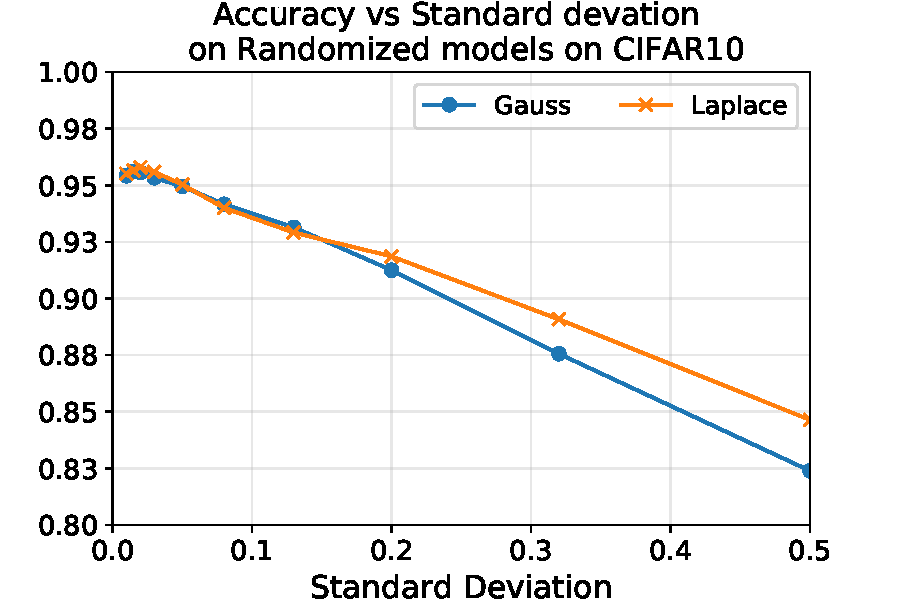
\includegraphics[scale=0.55]{figures/appendix/ap3-randomized_inference/acc_sd_CIFAR10.pdf}
  \caption{Impact of the standard deviation of the injected noise on accuracy in a randomized model on CIFAR-10 dataset with a Wide ResNet architecture.} 
  \label{figure:ap3-acc_sd_CIFAR10}
  \vspace{0.8cm}
  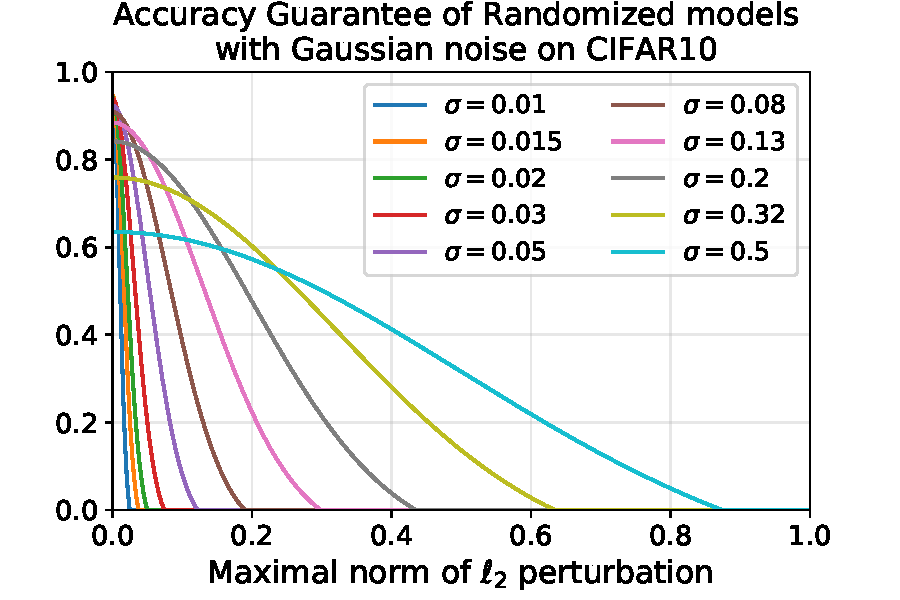
\includegraphics[scale=0.55]{figures/appendix/ap3-randomized_inference/gauss_certif_CIFAR10.pdf}
\caption{Illustration of the guaranteed accuracy of different randomized models with Gaussian noises given the norm of the adversarial perturbation.}
  \label{figure:ap3-gauss_certif_CIFAR10}
  \vspace{0.8cm}
  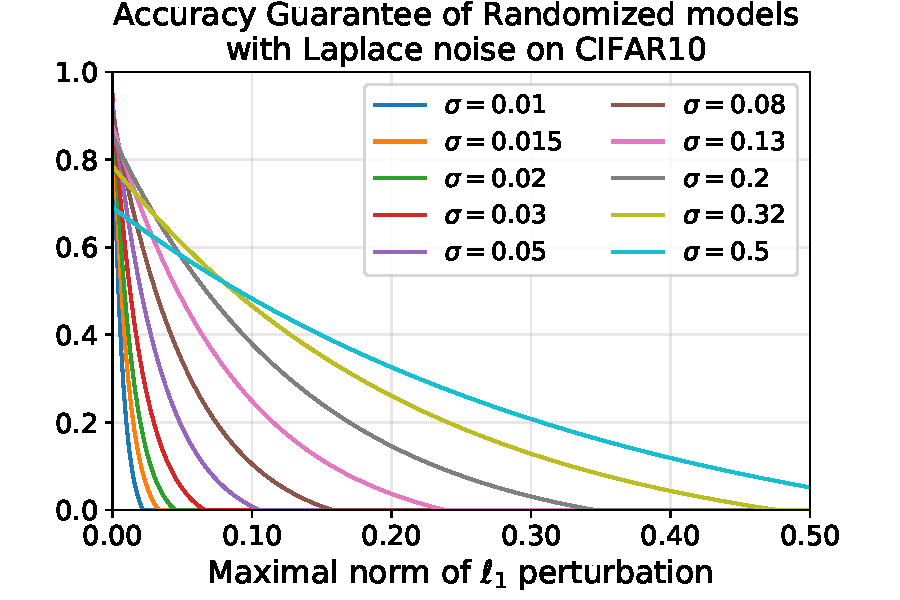
\includegraphics[scale=0.55]{figures/appendix/ap3-randomized_inference/laplace_certif_CIFAR10.pdf}
  \caption{Illustration of the guaranteed accuracy of different randomized models with Laplace noises given the norm of the adversarial perturbation.}
  \label{figure:ap3-laplace_certif_CIFAR10}
  \label{figure:ap3-cifar10_results}
\end{figure}
}


\paragraph{Trade-off between accuracy and intensity of noise (Q2.1):}

When injecting noise as a defense mechanism, regardless of the distribution it is drawn from, we observe (as in Figure~\ref{figure:ap3-acc_sd_CIFAR10}) that the accuracy decreases when the noise intensity grows.
In that sense, noise needs to be calibrated to preserve both accuracy and robustness against adversarial attacks, \ie, it needs to be large enough to preserve robustness and small enough to preserve accuracy.
Figure~\ref{figure:ap3-acc_sd_CIFAR10} shows the loss of accuracy on CIFAR10 from $0.95$ to $0.82$ (respectively $0.95$ to $0.84$) with noise drawn from a Gaussian distribution (respectively Laplace) with a standard deviation from $0.01$ to $0.5$.
Figure~\ref{figure:ap3-gauss_certif_CIFAR10} and \ref{figure:ap3-laplace_certif_CIFAR10} illustrate the theoretical lower bound on accuracy under attack of Theorem~\ref{theorem:ap3-bound} for different distributions and standard deviations.
The term in entropy of Theorem~\ref{theorem:ap3-bound} has been estimated using a Monte Carlo method with $10^4$ simulations.
The trade-off between accuracy and robustness from Theorem~\ref{theorem:ap3-bound} thus appears \wrt the noise intensity.
With small noises, the accuracy is high, but the guaranteed accuracy drops fast \wrt the magnitude of the adversarial perturbation.
Conversely, with bigger noises, the accuracy is lower but decreases slowly \wrt the magnitude of the adversarial perturbation.
These Figures also show that Theorem~\ref{theorem:ap3-bound} gives strong accuracy guarantees against small adversarial perturbations.
Next paragraph shows that in practice, randomized networks achieve much higher accuracy under attack than the theoretical bound, and keep this accuracy against much larger perturbations.


\paragraph{Performance of randomized networks under attacks and comparison to state of the art (Q2.2):}

While Figure~\ref{figure:ap3-gauss_certif_CIFAR10} and \ref{figure:ap3-laplace_certif_CIFAR10} illustrated a theoretical robustness against growing adversarial perturbations, Table~\ref{table:ap3-accuracy_under_attack} illustrates this trade-off experimentally.
It compares the accuracy obtained under attack by a deterministic network with the one obtained by randomized networks with Gaussian and Laplace noises both with low ($0.01$) and high ($0.5$) standard deviations.
Randomized networks with a small noise lead to no loss in accuracy with a small robustness while high noise leads to a higher robustness at the expense of loss of accuracy ($\sim11$ points). 

\begin{table}[t]
  \centering
  \begin{tabular}{lccccc}
    \toprule
    \textbf{Distribution} & \textbf{Sd} & \textbf{Natural} & \textbf{$\ell_1$ EAD 60} & \textbf{$\ell_2$ C\&W 60} & \textbf{$\ell_\infty$ PGD 20} \\
    \midrule
    \multicolumn{1}{c}{--} & -- & 0.958 & 0.035 & 0.034 & 0.384 \\
    \midrule
    \multirow{2}[0]{*}{Normal} & 0.01 & 0.954 & 0.193 & 0.294 & 0.408 \\
	  & 0.50 & 0.824 & 0.448 & 0.523 & 0.587 \\
    \midrule
    \multirow{2}[0]{*}{Laplace} & 0.01 & 0.955 & 0.208 & 0.313 & 0.389 \\
	  & 0.50 & 0.846 & 0.464 & 0.494 & 0.589 \\
    \bottomrule
  \end{tabular}%
  \caption{Accuracy under attack on the CIFAR-10 dataset with a randomized Wide ResNet architecture. We compare the accuracy on natural images and under attack with different noise over 3 iterative attacks (the number of steps is next to the name) made with 80 Monte Carlo simulations to compute EoT attacks. The first line is the baseline, no noise has been injected.}
  \label{table:ap3-accuracy_under_attack}%
\end{table}%

% \begin{table}[t]
%   \label{Results}
%   \centering
%   \begin{tabular}{ccccccc}
%     \toprule
%     & & \multirow{2}[0]{*}{\textbf{Madry et al.}} & \multirow{2}[0]{*}{\textbf{Normal 0.32}} & \multirow{2}[0]{*}{\textbf{Laplace 0.32}} & \multirow{2}[0]{*}{\textbf{Normal 0.5}} & \multirow{2}[0]{*}{\textbf{Laplace 0.5}} \\
%      \textbf{Attack} & \textbf{Steps} & & & \\
%     \midrule
%     --  & -- & 0.873 & 0.876 & 0.891 & 0.824 & 0.846 \\ 
%     $\ell_\infty$ -- PGD & 20 & 0.456 & 0.566 & 0.576 & 0.587 & 0.589 \\
%     $\ell_2$ -- C\&W & 30 & 0.468 & 0.512 & 0.502 & 0.489 & 0.479 \\
%     \bottomrule
%   \end{tabular}
%   \caption{Accuracy under attack of randomized neural network with different distributions and standard deviations versus adversarial training by~\citet{madry2018towards}. The PGD attack has been made with 20 step, an epsilon of 0.06 and a step size of 0.006 (input space between $-1$ and $+1$). The Carlini\&Wagner attack uses 30 steps, 9 binary search steps and a 0.01 learning rate. The first line refers to the baseline without attack.}
%   \label{table:madry_vs_random}
% \end{table}


\begin{table}[ht]
  \centering
  \begin{tabular}{cccccccccc}
    \toprule
    \multirow{2}{*}{\textbf{Attack}} & \multirow{2}{*}{\textbf{Steps}} & & \multirow{2}[0]{*}{\textbf{Madry et al.}} & &    \multicolumn{2}{c}{\textbf{Normal}} &  & \multicolumn{2}{c}{\textbf{Laplace}} \\
    \cmidrule{6-7} \cmidrule{9-10}
    & & & & & \textbf{0.32} & \textbf{0.5} &  & \textbf{0.32} & \textbf{0.5} \\
    \midrule
    --                    & -- & & 0.873 & & 0.876 & 0.824 & & 0.891 & 0.846 \\ 
    $\ell_\infty$ -- PGD  & 20 & & 0.456 & & 0.566 & 0.587 & & 0.576 & 0.589 \\
    $\ell_2$ -- C\&W      & 30 & & 0.468 & & 0.512 & 0.489 & & 0.502 & 0.479 \\
    \bottomrule
  \end{tabular}
  \caption{Accuracy under attack of randomized neural network with different distributions and standard deviations versus adversarial training by~\citet{madry2018towards}. The PGD attack has been made with 20 step, an epsilon of 0.06 and a step size of 0.006 (input space between $-1$ and $+1$). The Carlini\&Wagner attack uses 30 steps, 9 binary search steps and a 0.01 learning rate. The first line refers to the baseline without attack.}
  \label{table:madry_vs_random}
\end{table}

Finally, Table~\ref{table:madry_vs_random} compares the accuracy and the accuracy under attack of randomized networks with Gaussian and Laplace distributions for different standard deviations against adversarial training from~\citet{madry2018towards}.
We observe that the accuracy on natural images of both noise injection methods are similar to the one from~\citet{madry2018towards}.
Moreover, both methods are more robust than adversarial training to PGD and C\&W attacks.
As with all the experiments, to construct an EoT attack,  we use 80 Monte Carlo simulations at every step of PGD and C\&W attacks.
These experiments show that randomized defenses can be competitive given the intensity of noise injected in the network.
Note that these experiments have been led with $\EoT$ of size 80.
For much bigger sizes of $\EoT$ these results would be mitigated.
Nevertheless, the accuracy would never drop under the bounds illustrated in the Figures~\ref{figure:ap3-gauss_certif_CIFAR10} and \ref{figure:ap3-laplace_certif_CIFAR10}, since Theorem~\ref{theorem:ap3-bound} gives a bound that on the worst case attack strategy (including $\EoT$).


%%%%%%%%%%%%%%%%%%%%%%%%%%%%%%%%%%%%%%%%%%%%%%%%%%%%%%%%%%%%%%%%%%%%%%%%%%%%%%%
\section{Concluding Remarks}
\label{section:ap3-conclusion_remarks}
%%%%%%%%%%%%%%%%%%%%%%%%%%%%%%%%%%%%%%%%%%%%%%%%%%%%%%%%%%%%%%%%%%%%%%%%%%%%%%%

This chapter brings new contributions to the field of provable defenses to adversarial attacks.
Principled answers have been provided to key questions on the interest of randomization techniques, and on their loss of accuracy under attack.
The obtained bounds have been illustrated in practice by conducting thorough experiments on baseline datasets such as CIFAR and ImageNet.
We show in particular that a simple method based on injecting noise drawn from the Exponential family is competitive compared to baseline approaches while leading to provable guarantees.
Future work will focus on investigating other noise distributions belonging or not to the Exponential family, combining randomization with more sophisticated defenses and on devising new tight bounds on the adversarial generalization gap.




  %   %%%%%%%%%%%%%%%%%%%%%%%%%%%%%%%%%%%%%%%%%%%%%%%%%%%%%%%%%%%%%%%%%%%%%%%%%%%%%%%
\chapter{Advocating for Multiple Defense Strategies against Adversarial Examples}
\label{appendix:ap4-advocating_multiple_defense_strategies_against_adversarial_examples}
%%%%%%%%%%%%%%%%%%%%%%%%%%%%%%%%%%%%%%%%%%%%%%%%%%%%%%%%%%%%%%%%%%%%%%%%%%%%%%%
\localtoc


\vspace{\fill}

\emph{
This Appendix concerns a collaboration with Rafael Pinot, Laurent Meunier and Benjamin Negrevergne.
This work has been published in the European Conference on Machine Learning Workshop for CyberSecurity.
It conducts a geometrical analysis of defense mechanisms designed to protect neural networks against.
This work shows that neural networks designed to be robust against one type of adversarial example offer poor against other types of attacks.
}

\vspace{\fill}


%%%%%%%%%%%%%%%%%%%%%%%%%%%%%%%%%%%%%%%%%%%%%%%%%%%%%%%%%%%%%%%%%%%%%%%%%%%%%%%
\section{Introduction}
\label{section:ap4-introduction}
%%%%%%%%%%%%%%%%%%%%%%%%%%%%%%%%%%%%%%%%%%%%%%%%%%%%%%%%%%%%%%%%%%%%%%%%%%%%%%%




% Deep neural networks achieve state-of-the-art performances in a variety of domains such as natural language processing~\cite{radford2018Language}, image recognition~\cite{he2016deep} and speech recognition~\cite{hinton2012deep}.
% However, it has been shown that such neural networks are vulnerable to \emph{adversarial examples}, \ie, imperceptible variations of the natural examples, crafted to deliberately mislead the models~\cite{globerson2006nightmare,biggio2013evasion,szegedy2013intriguing}.
% Since their discovery, a variety of algorithms have been developed to generate adversarial examples (\aka attacks), for example FGSM \cite{goodfellow2014explaining}, PGD \cite{madry2018towards} and C\&W \cite{carlini2017towards}, to mention the most popular ones.

We have seen that deep neural networks are vulnerable to \emph{adversarial examples}.
Because it is difficult to characterize the space of visually imperceptible variations of a natural image, existing adversarial attacks use surrogates that can differ from one attack to another.
For example, \citet{goodfellow2014explaining} use the $\linf$ norm to measure the distance between the original image and the adversarial image whereas \citet{carlini2017towards} use the $\ltwo$ norm.
When the input dimension is low, the choice of the norm is of little importance because the $\linf$ and $\ltwo$ balls overlap by a large margin, and the adversarial examples lie in the same space.
An important insight in this chapter is to observe that the overlap between the two balls diminishes exponentially quickly as the dimensionality of the input space increases.
For typical image datasets with large dimensionality, the two balls are mostly disjoint.
As a consequence, the $\linf$ and the $\ltwo$ adversarial examples lie in different areas of the space, and it explains why $\linf$ defense mechanisms perform poorly against $\ltwo$ attacks and vice versa. 

Building on this insight, we advocate for designing models that incorporate defense mechanisms against both $\linf$ and $\ltwo$ attacks and review several ways of mixing existing defense mechanisms.
In particular, we evaluate the performance of \emph{Mixed Adversarial Training} (MAT)~\cite{goodfellow2014explaining} which consists of  augmenting training batches using \emph{both} $\linf$ and $\ltwo$ adversarial examples, and {\em Randomized Adversarial Training} (RAT)~\cite{salman2019provably}, a solution to benefit from the advantages of both $\linf$ adversarial training, and $\ltwo$ randomized defense. 


%%%%%%%%%%%%%%%%%%%%%%%%%%%%%%%%%%%%%%%%%%%%%%%%%%%%%%%%%%%%%%%%%%%%%%%%%%%%%%%
\section{No Free Lunch for Adversarial Defenses}
\label{section:ap4-no_free_lunch}
%%%%%%%%%%%%%%%%%%%%%%%%%%%%%%%%%%%%%%%%%%%%%%%%%%%%%%%%%%%%%%%%%%%%%%%%%%%%%%%

In this Section, we show both theoretically and empirically that defenses mechanisms intending to defend against $\linf$ attacks cannot provide suitable defense against $\ltwo$ attacks.
Our reasoning is perfectly general; hence we can similarly demonstrate the reciprocal statement, but we focus on this side for simplicity.


\begin{figure}
   \centering
   \begin{subfigure}[t]{0.32\textwidth}
       \centering
       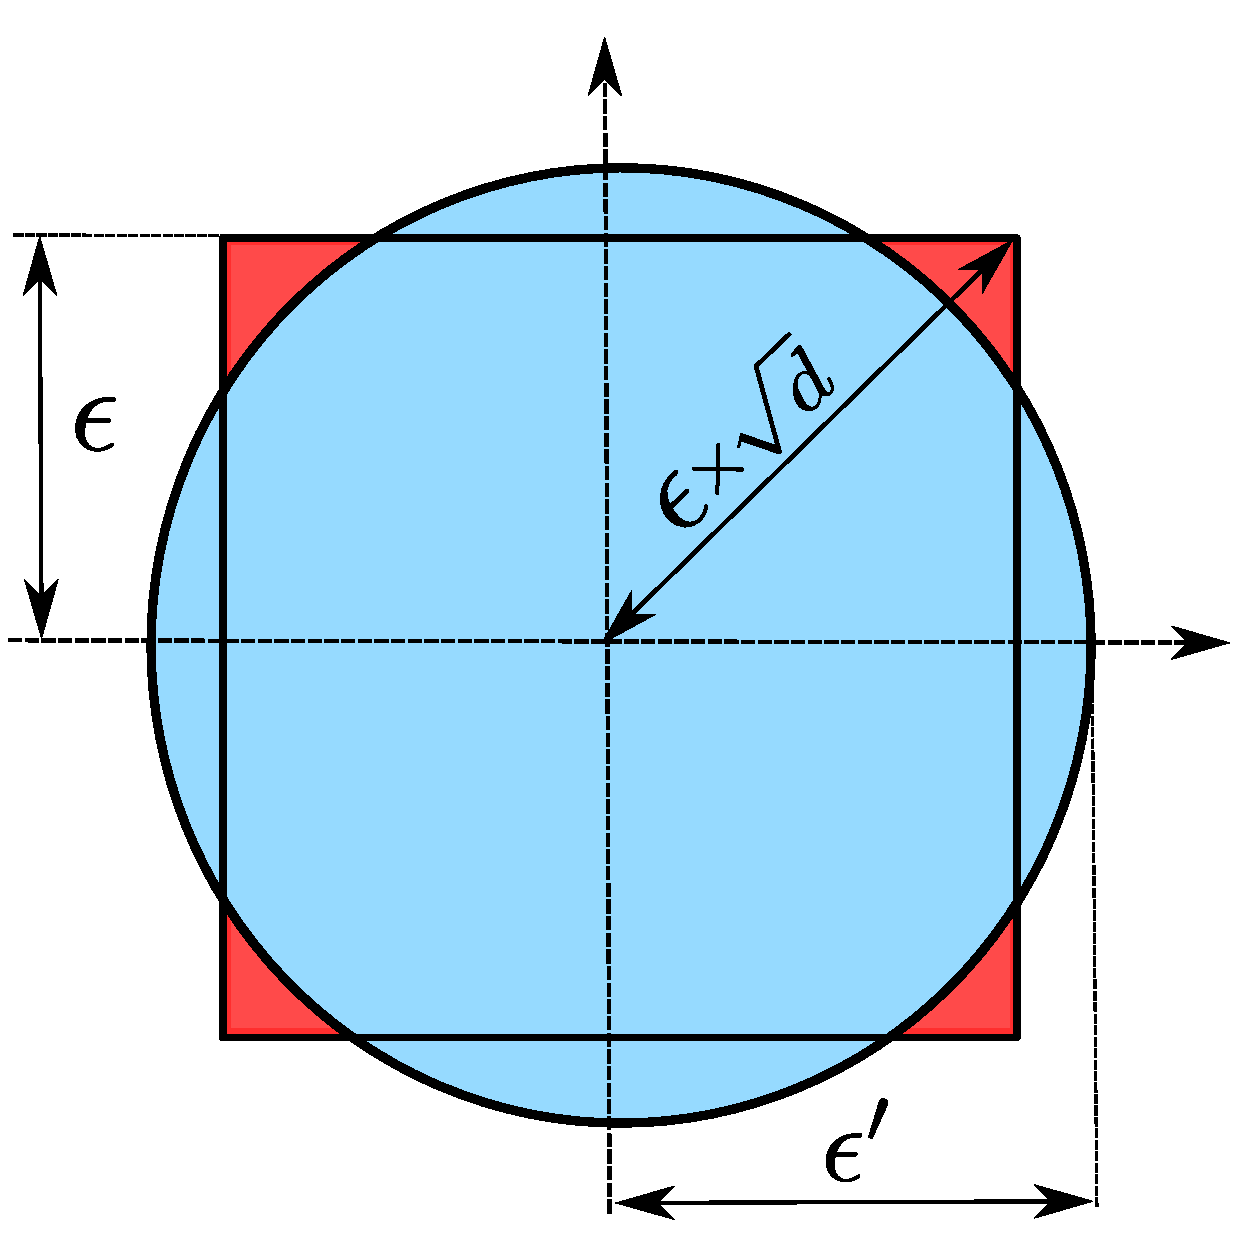
\includegraphics[scale=0.22]{figures/appendix/ap4-advocating_for_multiple_defense_strategies/ball_inclusion_adversarial_training.pdf}
       \caption{2D representation of the $\linf$ and $\ltwo$ balls of respective radius $\epsilon$ and $\epsilon'$}
       \label{figure:ap4-ball_inclusion_adversarial_training}
   \end{subfigure}
   \hfill
   \begin{subfigure}[t]{0.32\textwidth}
       \centering
       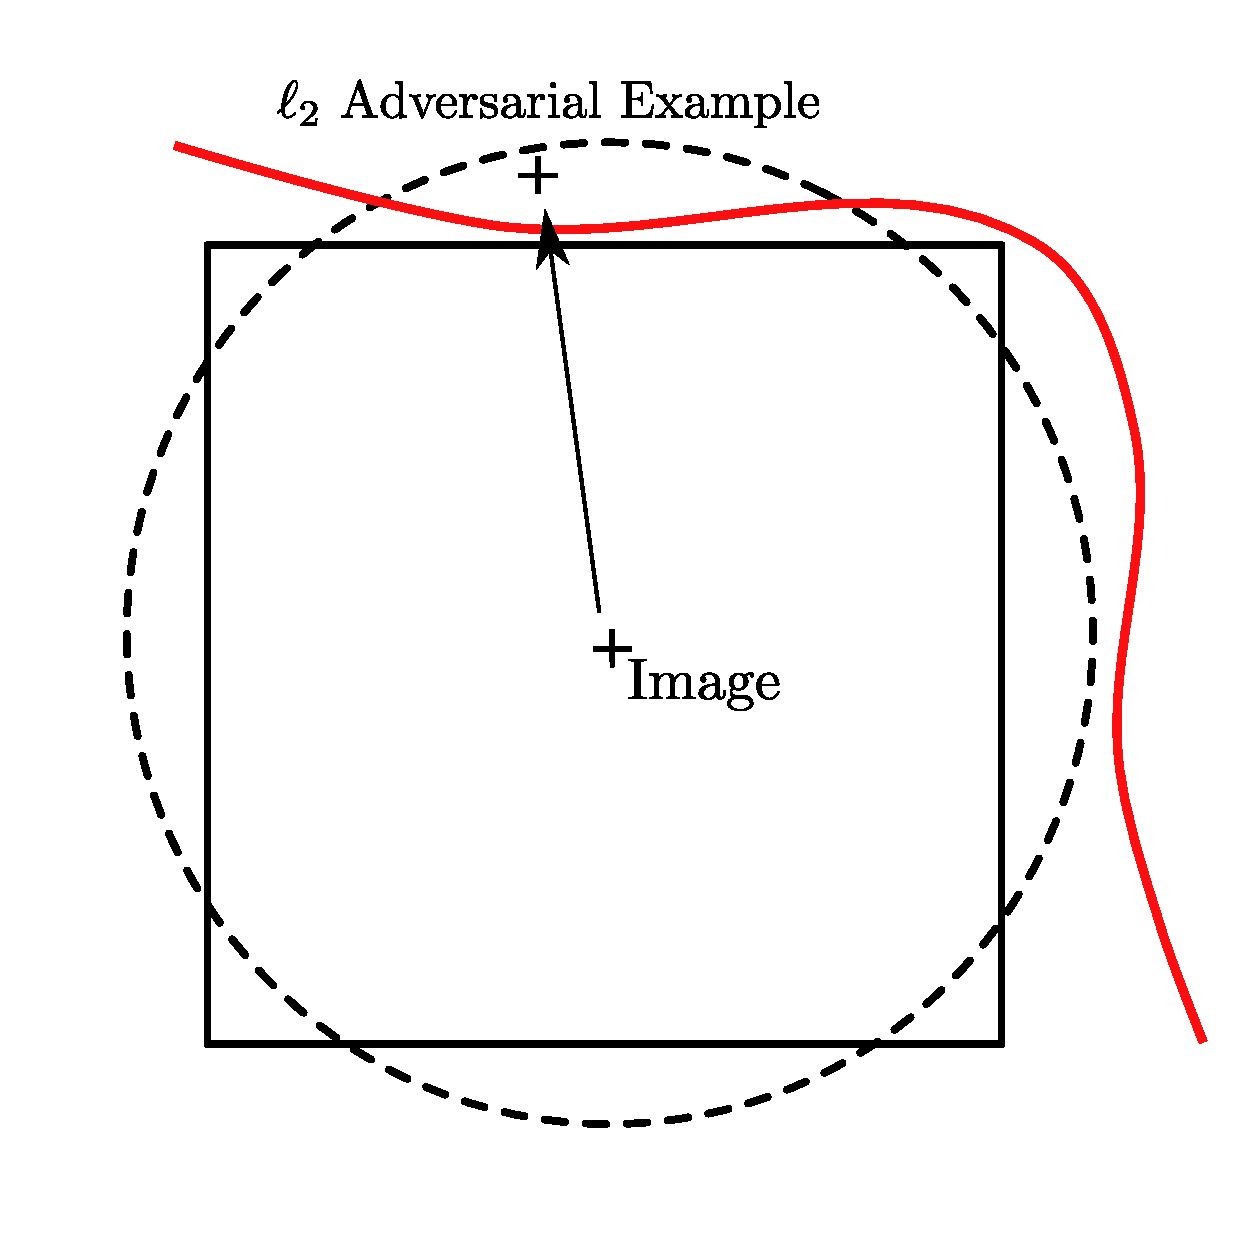
\includegraphics[scale=0.22]{figures/appendix/ap4-advocating_for_multiple_defense_strategies/ball_adversarial_l2.pdf}
       \caption{A classifier trained with $\linf$ adversarial perturbations  (materialized by the red line) remains vulnerable to $\ltwo$ attacks.}
       \label{figure:ap4-ball_adversarial_l2}
   \end{subfigure}
   \hfill
   \begin{subfigure}[t]{0.32\textwidth}
       \centering
       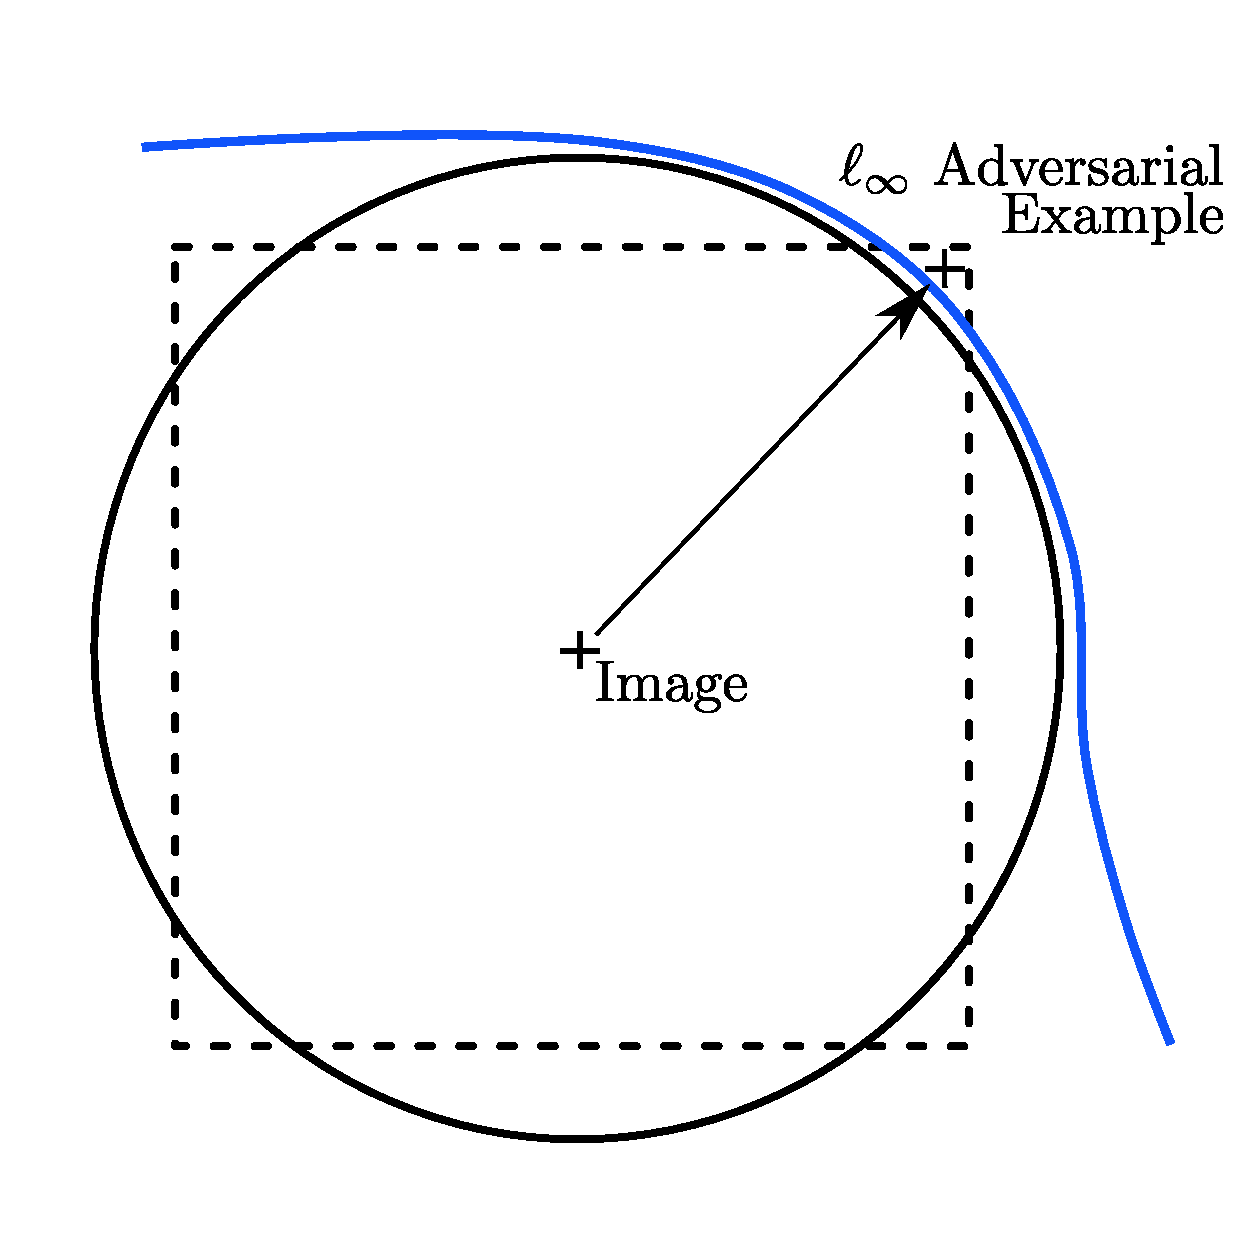
\includegraphics[scale=0.22]{figures/appendix/ap4-advocating_for_multiple_defense_strategies/ball_adversarial_linf.pdf}
       \caption{A classifier trained with $\ltwo$ adversarial perturbations (materialized by the blue line) remains vulnerable to $\linf$ attacks.}
       \label{figure:ap4-ball_adversarial_linf}
   \end{subfigure}
   \caption{2-dimensional representation of $\linf$ and $\ltwo$ balls}
   % \caption{Left: 2D representation of the $\linf$ and $\ltwo$ balls of respective radius $\epsilon$ and $\epsilon'$. 
   %  Middle: a classifier trained with $\linf$ adversarial perturbations  (materialized by the red line) remains vulnerable to $\ltwo$ attacks. 
   %  Right: a classifier trained with $\ltwo$ adversarial perturbations (materialized by the blue line) remains vulnerable to $\linf$ attacks.}
\end{figure}


%%%%%%%%%%%%%%%%%%%%%%%%%%%%%%%%%%%%%%%%%%%%%%%%%%%%%%%%%%%%%%%%%%%%%%%%%%%%%%%
\subsection{Theoretical analysis}
\label{subsection:ap4-theoretical_analysis}
%%%%%%%%%%%%%%%%%%%%%%%%%%%%%%%%%%%%%%%%%%%%%%%%%%%%%%%%%%%%%%%%%%%%%%%%%%%%%%%

Let us consider a classifier $f_{\infty}$ that is provably robust against adversarial examples with maximum $\linf$ norm of value $\epsilon_\infty$.
It guarantees that for any input-output pair $(x,y) \sim \Dset$ and for any perturbation $\tau$ such that $\norm{\tau}_\infty \leq \epsilon_\infty$, $f_{\infty}$ is not misled by the perturbation, \ie, $f_{\infty}(x + \tau) = f_{\infty}(x)$.
We now focus our study on the performance of this classifier against adversarial examples bounded with a $\ltwo$ norm of value $\epsilon_2$.
Using Figure~\ref{figure:ap4-ball_inclusion_adversarial_training}, we observe that any $\ltwo$ adversarial example that is also in the $\linf$ ball, will not fool $f_{\infty}$.
Conversely, if it is outside the ball, we have no guarantee.

To characterize the probability that such an  $\ltwo$ perturbation fools an $\linf$ defense mechanism in the general case (\emph{i.e.}, any dimension $d$), we measure the ratio between the volume of the intersection of the $\linf$ ball of radius $\epsilon_\infty$ and the $\ltwo$ ball of radius $\epsilon_2$. As Theorem~\ref{theorem:ap4-nullvolume} shows, this ratio depends on the dimensionality $d$ of the input vector $x$, and  rapidly converges to zero when $d$ increases. 
Therefore a defense mechanism that protects against all $\linf$ bounded adversarial examples is unlikely to be efficient against $\ltwo$ attacks.


\begin{theorem}[Probability of the intersection goes to $0$] ~\\
Let
\begin{equation}
  B_{2,d}(\epsilon) \triangleq \left \{\tau \in \Rbb^d \ |\  \norm{\tau}_2 \leq \epsilon \right \}
\end{equation}
and
\begin{equation}
  B_{\infty,d}(\epsilon') \triangleq \left \{\tau \in \Rbb^d \ |\  \norm{\tau}_\infty \leq \epsilon' \right\}.
\end{equation}
If for all $d$, we select $\epsilon$ and $\epsilon$' such that $\Vol\left(B_{2,d}(\epsilon)\right) = \Vol\left(B_{\infty,d}(\epsilon')\right)$, then
\begin{equation}
  \frac{\Vol\left(B_{2,d}(\epsilon)\bigcap B_{\infty,d}(\epsilon')\right)}{\Vol\left(B_{\infty,d}(\epsilon')\right)} \rightarrow 0 \text{ when } d\rightarrow \infty.
\end{equation}
\label{theorem:ap4-nullvolume}
\end{theorem} 

\begin{proof}[\Cref{theorem:ap4-nullvolume}] 
Without loss of generality, let us fix $\epsilon = 1$. One can show that for all $d$, 
\begin{equation}
    \Vol\left( B_{2,d}\left(\frac{2}{\sqrt{\pi}}\Gamma\left(\frac{d}{2}+1\right)^{1/d}\right)\right) = \Vol\left(B_{\infty,d}\left(1\right)\right)
\end{equation}
where $\Gamma$ is the gamma function. Let us denote 
\begin{equation}
    r_2(d)=\frac{2}{\sqrt{\pi}}\Gamma\left(\frac{d}{2}+1\right)^{1/d}.
\end{equation}
Then, thanks to Stirling's formula
\begin{equation}
    r_2(d)\sim \sqrt{\frac{2}{\pi e}} d^{1/2}.
\end{equation}
Finally, if we denote $\mathcal{U}_S$, the uniform distribution on set $S$, by using  Hoeffding inequality between Equation~\ref{equation:ap4-hoeffding1} and \ref{equation:ap4-hoeffding2}, we get:
\begin{align}
  \frac{\Vol(B_{2,d}(r_2(d)) \bigcap B_{\infty,d}(1))}{\Vol(B_{\infty,d}(1))} &= \Pbb_{x \sim \mathcal{U}_{B_{\infty,d}(1)}} \left[ x \in B_{2,d}(r_2(d)) \right] \\
  &= \Pbb_{x \sim \mathcal{U}_{B_{\infty,d}(1)}} \left[ \sum_{i=1}^d |x_i|^2 \leq r_2^2(d) \right] \\
  &\leq \exp{- d^{-1} \left( r_2^2(d) - d \Ebb |x_1|^2 \right)^2} \label{equation:ap4-hoeffding1} \\
  &\leq \exp{-\left( \frac{2}{\pi e}-\frac23\right)^2d+o(d)} \label{equation:ap4-hoeffding2}.
\end{align}
Then the ratio between the volume of the intersection of the ball and the volume of the ball converges towards $0$ when $d$ goes to $\infty$.
\end{proof}

Theorem~\ref{theorem:ap4-nullvolume} states that, when $d$ is large enough, $\ltwo$ bounded perturbations have a null probability of being also in the $\linf$ ball of the same volume.
As a consequence, for any value of $d$ that is large enough, a defense mechanism that offers full protection against $\linf$ adversarial examples is not guaranteed to offer any protection against $\ltwo$ attacks \footnote{Theorem~\ref{theorem:ap4-nullvolume} can easily be extended to any two balls with different norms. For clarity, we restrict to the case of $\linf$ and $\ltwo$ norms.}.

\begin{table}[ht]
  \centering
  \begin{tabular}{c r r r l}
    \toprule
    \textbf{Dataset\ } & \phantom{....} & \textbf{Dim.} $\mathbf{(d)}$ & \phantom{....} & \textbf{Vol. of the intersection }\\
    \midrule
    -- & & 2\ \ & & $10^{-0.009}$ \quad ($\approx$ 0.98) \\
    MNIST & & 784\ \  & & $10^{-144}$\\
    CIFAR & & 3072\ \ & &  $10^{-578}$\\
    ImageNet & & 150528\ \ & & $10^{-28946}$\\
    \bottomrule
  \end{tabular}
  \caption{ Bounds of Theorem~\ref{theorem:ap4-nullvolume} on the volume of the intersection of  $\ltwo$ and $\linf$ balls at equal volume for typical image classification datasets. When $d=2$, the bound is $ 10^{-0.009}\approx 0.98$.}
  \label{table:ap4-datadim}
\end{table}

Note that this result defeats the 2-dimensional intuition: if we consider a 2 dimensional problem setting, the $\linf$ and the $\ltwo$ balls have an important overlap (as illustrated in Figure~\ref{figure:ap4-ball_inclusion_adversarial_training}) and the probability of sampling at the intersection of the two balls is bounded by approximately 98\%.
However, as we increase the dimensionality $d$, this probability quickly becomes negligible, even for very simple image datasets such as MNIST.
An instantiation of  the bound for classical image datasets is presented in Table~\ref{table:ap4-datadim}.
The probability of sampling at the intersection of the $\linf$ and $\ltwo$ balls is close to zero for any realistic image setting.
In large dimensions, the volume of the corner of the $\linf$ ball is much bigger than it appears in Figure~\ref{figure:ap4-ball_inclusion_adversarial_training}.


%%%%%%%%%%%%%%%%%%%%%%%%%%%%%%%%%%%%%%%%%%%%%%%%%%%%%%%%%%%%%%%%%%%%%%%%%%%%%%%
\subsection{No Free Lunch in Practice}
\label{subsection:ap4-no_free_lunch_in_practice}
%%%%%%%%%%%%%%%%%%%%%%%%%%%%%%%%%%%%%%%%%%%%%%%%%%%%%%%%%%%%%%%%%%%%%%%%%%%%%%%

Our theoretical analysis shows that if adversarial examples were uniformly distributed in a high-dimensional space, then any mechanism that perfectly defends against $\linf$ adversarial examples has a null probability of protecting against $\ltwo$-bounded adversarial attacks.
Although existing defense mechanisms do not necessarily assume such a distribution of adversarial examples, we demonstrate that whatever distribution they use, it offers no favorable bias with respect to the result of Theorem~\ref{theorem:ap4-nullvolume}.
As we discussed in Chapter~\ref{chapter:ch5-lipschitz_bound}, there are two distinct attack settings: loss maximization (PGD) and perturbation minimization (C\&W).
Our analysis is mainly focusing on loss maximization attacks.
However, these attacks have a very strict geometry\footnote{Due to the projection operator, all PGD attacks saturate the constraint, which makes them all lies in a very small part of the ball.}.
This is why, to present a deeper analysis of the behavior of adversarial attacks and defenses, we also present a set of experiments that use perturbation minimization attacks.

\begin{table}[htbp]
  \centering 
  \begin{tabular}{lccccccc}
    \toprule
    &  & \multicolumn{2}{c}{\textbf{Attack PGD-}$\ltwo$} & & \multicolumn{2}{c}{\textbf{Attack PGD-}$\linf$} \\
  \cmidrule{3-4} \cmidrule{6-7}
  &  & \textbf{Unprotected} & \textbf{AT-}$\linf$ & & \textbf{Unprotected} & \textbf{AT-}$\ltwo$ \\
    \midrule
    \textbf{Average $\ltwo$ norm} &   & 0.830 & 0.830 &   & 1.400 & 1.640 \\
    \textbf{Average $\linf$ norm} &   & 0.075 & 0.200 &   & 0.031 & 0.031 \\
    \bottomrule
  \end{tabular}%
  \caption{Average norms of PGD-$\ltwo$ and PGD-$\linf$ adversarial examples with and without $\linf$ adversarial training on CIFAR-10 ($d=3072$).}
  \label{table:ap4-mean_norm_pgd_attack}
\end{table}%

\paragraph{Adversarial training vs. loss maximization attacks}

To demonstrate that $\linf$ adversarial training is not robust against PGD-$\ltwo$ attacks we measure the evolution of $\ltwo$ norm of adversarial examples generated with PGD-$\linf$ between an unprotected model and a model trained with AT-$\linf$, \ie, AT where adversarial examples are generated with PGD-$\linf$ \footnote{To do so, we use the same experimental setting as in Section~\ref{section:ap4-reviewing_defenses_against_multiple_attacks} with $\epsilon_\infty$ and $\epsilon_2$ such that the volumes of the two balls are equal.}. 
Results are presented in  Table~\ref{table:ap4-mean_norm_pgd_attack}.

The analysis is unambiguous: the average $\linf$ norm of a bounded $\ltwo$ perturbation more than double between an unprotected model and a model trained with AT PGD-$\linf$. This phenomenon perfectly reflects the illustration of Figure~\ref{figure:ap4-ball_adversarial_linf}. The attack will generate an adversarial example on the corner of the $\linf$ ball thus increasing the $\linf$ norm while maintaining the same $\ltwo$ norm. 
We can observe the same phenomenon with AT-$\ltwo$ against PGD-$\linf$ attack (see Figure~\ref{figure:ap4-ball_adversarial_l2} and Table \ref{table:ap4-mean_norm_pgd_attack}). PGD-$\linf$ attack increases the $\ltwo$ norm while maintaining the same $\linf$ perturbation thus generating the perturbation in the upper area. 

As a consequence, we cannot expect adversarial training $\linf$ to offer any guaranteed protection against $\ltwo$ adversarial examples .

\paragraph{Adversarial training vs. perturbation minimization attacks.}
To better capture the behavior of $\ltwo$ adversarial examples, we now study the performances of an $\ltwo$ perturbation minimization attack (C\&W) with and without AT-$\linf$.
It allows us to understand in which area C\&W discovers adversarial examples and the impact of AT-$\linf$.
In high dimensions, the red corners (see Figure~\ref{figure:ap4-ball_inclusion_adversarial_training}) are very far away from the $\ltwo$ ball.
Therefore, we hypothesize that a large proportion of the $\ltwo$ adversarial examples will remain unprotected.
To validate this assumption, we measure the proportion of adversarial examples inside of the $\ltwo$ ball before and after $\linf$ adversarial training.
The results are presented in Figure~\ref{fig:calotte} (left: without adversarial training, right: with adversarial training). 

\begin{figure}[htb]
    \centering
    \begin{tikzpicture}[scale=0.7]
    \begin{groupplot}[group style={
                        group name=myplot,
			group size= 2 by 1,
		        horizontal sep=3cm},
                      grid style=dashed,
		      ymajorgrids=true]
       
    \nextgroupplot[
       stack plots=y,
       area style,
       ytick={0,5000,1000},
       ymin=0,
       ymax=10000,
       xmin=0.3,
       xmax=16.63,
       axis x line*=bottom,
       axis y line*=left,
       xtick={2,14},
       xticklabels={\Large $\epsilon'=\epsilon\phantom{\sqrt{d}}$, \Large $\epsilon'=\epsilon\times\sqrt{d}$},
       xtick style={draw=none}]
        \addplot table [x=eps,y=linf_ball] {figures/appendix/ap4-advocating_for_multiple_defense_strategies/data/ball_l2_base.dat}\closedcycle;
        \addplot table [x=eps,y=callote] {figures/appendix/ap4-advocating_for_multiple_defense_strategies/data/ball_l2_base.dat}\closedcycle;
        \addplot table [x=eps,y=outside] {figures/appendix/ap4-advocating_for_multiple_defense_strategies/data/ball_l2_base.dat}\closedcycle;

    \nextgroupplot[
       stack plots=y,
       area style,
       ytick={0,5000,1000},
       ymin=0,
       ymax=10000,
       xmin=0.3, 
       xmax=16.63,
       axis x line*=bottom,
       axis y line*=left,
       xtick={2,14},
       xticklabels={\Large $\epsilon'=\epsilon\phantom{\sqrt{d}}$, \Large $\epsilon'=\epsilon\times\sqrt{d}$},
       xtick style={draw=none}]
        \addplot table [x=eps,y=linf_ball] {figures/appendix/ap4-advocating_for_multiple_defense_strategies/data/ball_l2_at.dat}\closedcycle;
        \addplot table [x=eps,y=callote] {figures/appendix/ap4-advocating_for_multiple_defense_strategies/data/ball_l2_at.dat}\closedcycle;
        \addplot table [x=eps,y=outside] {figures/appendix/ap4-advocating_for_multiple_defense_strategies/data/ball_l2_at.dat}\closedcycle;

    \end{groupplot}
\end{tikzpicture}


    \caption{Comparison of the number of adversarial examples found by C\&W, inside the $\linf$ ball (lower, blue area), outside the $\linf$ ball but inside the $\ltwo$ ball (middle, red area) and outside the $\ltwo$ ball (upper gray area). $\epsilon$ is set to $0.3$ and $\epsilon'$ varies along the x-axis. Left: without adversarial training, right: with adversarial training. Most adversarial examples have shifted from the $\linf$ ball to the cap of the $\ltwo$ ball, but remain at the same $\ltwo$ distance from the original example.}
    \label{fig:calotte}
\end{figure}

On both charts, the blue area represents the proportion of adversarial examples that are inside the $\linf$ ball.
The red area represents the adversarial examples that are outside the $\linf$ ball but still inside the $\ltwo$ ball (valid $\ltwo$ adversarial examples).
Finally, the brown-beige area represents the adversarial examples that are beyond the $\ltwo$ bound.
The radius $\epsilon'$ of the $\ltwo$ ball varies along the x-axis from $\epsilon'$ to $\epsilon' \sqrt{d}$.
On the left chart (without adversarial training) most $\ltwo$ adversarial examples generated by C\&W are inside both balls.
On the right chart most of the adversarial examples have been shifted out the $\linf$ ball.
This is the expected consequence of $\linf$ adversarial training.
However, these adversarial examples remain in the $\ltwo$ ball, \ie, they are in the cap of the $\ltwo$ ball.
These examples are equally good from the $\ltwo$ perspective.
This means that even after adversarial training, it is still easy to find good $\ltwo$ adversarial examples, making the $\ltwo$ robustness of AT-$\linf$ almost null. 

%%%%%%%%%%%%%%%%%%%%%%%%%%%%%%%%%%%%%%%%%%%%%%%%%%%%%%%%%%%%%%%%%%%%%%%%%%%%%%%%
\section{Reviewing Defenses Against Multiple Attacks}
\label{section:ap4-reviewing_defenses_against_multiple_attacks}
%%%%%%%%%%%%%%%%%%%%%%%%%%%%%%%%%%%%%%%%%%%%%%%%%%%%%%%%%%%%%%%%%%%%%%%%%%%%%%%%

\begin{table}[ht]
  \centering
  \tabcolsep=0.13cm
  {\small
  \begin{tabular}{lccccccccccccccccc}
    \toprule
     & & \multirow{2}{*}{\textbf{Baseline}} & & \multicolumn{2}{c}{\textbf{AT}} & & \multicolumn{2}{c}{\textbf{MAT}} & & \multicolumn{2}{c}{\textbf{NI}} & & \multicolumn{2}{c}{\textbf{RAT}-$\linf$} & & \multicolumn{2}{c}{\textbf{RAT}-$\ltwo$} \\
    \cmidrule{5-6} \cmidrule{8-9} \cmidrule{11-12} \cmidrule{14-15} \cmidrule{17-18}
     & & & & $\linf$ & $\ltwo$ &   & Max & Rand &   & $\mathcal{N}$ & $\mathcal{U}$ &   & $\mathcal{N}$ & $\mathcal{U}$ &   & $\mathcal{N}$ & $\mathcal{U}$ \\
    \midrule
    \textbf{Natural}     &   & 0.94 &   & 0.85 & 0.85 &   & 0.80 & 0.80 &   & 0.79 & 0.87 &   & 0.74 & 0.80 &   & 0.79 & 0.87 \\
    \textbf{PGD-$\linf$} &   & 0.00 &   & 0.43 & 0.37 &   & 0.37 & 0.40 &   & 0.23 & 0.22 &   & 0.35 & 0.40 &   & 0.23 & 0.22 \\
    \textbf{PGD-$\ltwo$} &   & 0.00 &   & 0.37 & 0.52 &   & 0.50 & 0.55 &   & 0.34 & 0.36 &   & 0.43 & 0.39 &   & 0.34 & 0.37 \\
    \bottomrule
  \end{tabular}%
  }
  \caption{Comprehensive list of results consisting of the accuracy of several defense mechanisms against $\ltwo$ and $\linf$ attacks.}
  \label{table:ap4-results}
\end{table}%


Adversarial attacks have been an active topic in the machine learning community since their discovery~\cite{globerson2006nightmare, biggio2013evasion,szegedy2013intriguing}.
Many attacks have been developed.
Most of them solve a loss maximization problem with either $\linf$~\cite{goodfellow2014explaining,kurakin2016adversarial,madry2018towards}, $\ltwo$~\cite{carlini2017towards,kurakin2016adversarial,madry2018towards}, $\lone$~\cite{tramer2019adversarial} or $\lzero$~\cite{papernot2016limitations} surrogate norms.
As we showed, these norms are really different in high dimension.
Hence, defending against one norm-based attack is not sufficient to protect against another one. 
In order to solve this problem, we review several strategies to build defenses against multiple adversarial attacks.
These strategies are based on the idea that both types of defense must be used simultaneously in order for the classifier to be protected against multiple attacks.

%%%%%%%%%%%%%%%%%%%%%%%%%%%%%%%%%%%%%%%%%%%%%%%%%%%%%%%%%%%%%%%%%%%%%%%%%%%%%%%
\subsection{Experimental Setting}
\label{section:ap4-experimental_settings}
%%%%%%%%%%%%%%%%%%%%%%%%%%%%%%%%%%%%%%%%%%%%%%%%%%%%%%%%%%%%%%%%%%%%%%%%%%%%%%%

To compare the robustness provided by the different defense mechanisms, we use strong adversarial attacks and a conservative setting: the attacker has a total knowledge of the parameters of the model (white-box setting) and we only consider untargeted attacks  (a misclassification from one target to any other will be considered as adversarial).
To evaluate defenses based on Noise Injection, we use \emph{Expectation Over Transformation} (EOT), the rigorous experimental protocol  proposed by~\citet{athalye2017synthesizing} and later used by~\citet{athalye2018obfuscated,carlini2019evaluating} to identify flawed defense mechanisms. 

To attack the models, we use state-of-the-art algorithms PGD.
We run PGD with 20 iterations to generate adversarial examples and with 10 iterations when it is used for adversarial training.
The maximum $\linf$ bound is fixed to $0.031$ and the maximum $\ltwo$ bound is fixed to $0.83$.
We chose these values so that the $\linf$ and the $\ltwo$ balls have similar volumes.
Note that $0.83$ is slightly above the values typically used in previous publications in the area, meaning the attacks are stronger, and thus  more difficult to defend against.

All experiments are conducted on CIFAR-10 with the Wide-Resnet 28-10 architecture.
We use the training procedure and the hyper-parameters described in the original paper by~\citet{zagoruyko2016wide}.
Training time varies from 1 day (AT) to 2 days (MAT) on 4 GPUs-V100 servers. 


%%%%%%%%%%%%%%%%%%%%%%%%%%%%%%%%%%%%%%%%%%%%%%%%%%%%%%%%%%%%%%%%%%%%%%%%%%%%%%%
\subsection{MAT -- Mixed Adversarial Training}
\label{subsection:ap4-mixed_adversarial_training}
%%%%%%%%%%%%%%%%%%%%%%%%%%%%%%%%%%%%%%%%%%%%%%%%%%%%%%%%%%%%%%%%%%%%%%%%%%%%%%%

Earlier results have shown that AT-$\lp$ improves the robustness against corresponding $\lp$-bounded adversarial examples, and the experiments we present in this section corroborate this observation (See Table~\ref{table:ap4-results}, column: AT).
Building on this, it is natural to examine the efficiency of \emph{Mixed Adversarial Training} (MAT) against mixed $\linf$ and $\ltwo$ attacks.
MAT is a variation of AT that uses both $\linf$-bounded adversarial examples and $\ltwo$-bounded adversarial examples as training examples.
As discussed by~\citet{tramer2019adversarial}, there are several possible strategies to mix the adversarial training examples.
The first strategy (MAT-Rand) consists in randomly selecting one adversarial example among the two most damaging $\linf$ and $\ltwo$, and to use it as a training example:

\paragraph{MAT-Rand}:
\begin{equation} \label{equation:ap4-mat_rand}
  \min_{\theta} \Ebb_{(x, y) \sim \Dset} \left[\Ebb_{p\sim\mathcal{U}({\{2, \infty\})}} \max_{\norm{\tau}_p \leq \epsilon} L \left( f_{\theta}(x+\tau), y \right) \right].
\end{equation}

An alternative strategy is to systematically train the model with the most damaging adversarial example ($\linf$ or $\ltwo$):
\paragraph{MAT-Max}:
\begin{equation} \label{equation:ap4-mat_max}
  \min_{\theta} \Ebb_{(x, y) \sim \Dset} \left[ \max_{p \in \{2, \infty\}} \max_{\norm{\tau}_p \leq \epsilon} L \left( f_{\theta}(x+\tau), y \right) \right].
\end{equation}

The accuracy of MAT-Rand and MAT-Max are reported in~\Cref{table:ap4-results} (Column: MAT).
As expected, we observe that MAT-Rand and MAT-Max offer better robustness both against PGD-$\ltwo$ and PGD-$\linf$ adversarial examples than the original AT does.
More  generally, we can see that AT is a good strategy against loss maximization attacks, and thus it is not surprising that MAT is a good strategy against mixed loss maximization attacks.
However efficient in practice, MAT (for the same reasons as AT) lacks theoretical arguments.
In order to get the best of both worlds, \citet{salman2019provably} proposed to mix adversarial training with randomization.  


%%%%%%%%%%%%%%%%%%%%%%%%%%%%%%%%%%%%%%%%%%%%%%%%%%%%%%%%%%%%%%%%%%%%%%%%%%%%%%%
\subsection{RAT -- Randomized Adversarial Training}
\label{subsection:ap4-randomized_adversarial_training}
%%%%%%%%%%%%%%%%%%%%%%%%%%%%%%%%%%%%%%%%%%%%%%%%%%%%%%%%%%%%%%%%%%%%%%%%%%%%%%%

We now examine the performance of Randomized Adversarial Training (RAT) first introduced by~\citet{salman2019provably}.
This technique mixes Adversarial Training with Noise Injection.
The corresponding loss function is defined as follows:
\begin{equation}
  \min_{\theta} \Ebb_{(\xvec, y) \sim \Dset} \left[ \max_{\norm{\tau}_p \leq \epsilon} L\left( \tilde{f}_{\theta}(\xvec+\tau), y)  \right) \right].
\end{equation}
where $\tilde{f}_\theta$ is a randomized neural network with noise injection as described in Appendix~\ref{appendix:ap3-theoretical_evidence_for_adversarial_robustness_through_randomization}, and $\norm{\ \cdot\ }_p$ define which kind of AT is used.
For each setting, we consider two noise distributions, Gaussian and Uniform as we did with NI.
We also consider two different Adversarial training AT-$\linf$ as well as AT-$\ltwo$. 

The results of RAT are reported in Table~\ref{table:ap4-results}~(Columns: RAT-$\linf$ and RAT-$\ltwo$).
We can observe that RAT-$\linf$ offers the best extra robustness with both noises, which is consistent with previous experiments, since AT is generally more effective against $\linf$ attacks whereas NI is more effective against $\ltwo$-attacks.
Overall, RAT-$\linf$ and a noise from uniform distribution offers the best performances but is still weaker than MAT-Rand.
These results are also consistent with the literature, since adversarial training (and its variants) is the best defense against adversarial examples so far.


%%%%%%%%%%%%%%%%%%%%%%%%%%%%%%%%%%%%%%%%%%%%%%%%%%%%%%%%%%%%%%%%%%%%%%%%%%%%%%%
\section{Concluding Remarks}
\label{section:ap4-conclusion}
%%%%%%%%%%%%%%%%%%%%%%%%%%%%%%%%%%%%%%%%%%%%%%%%%%%%%%%%%%%%%%%%%%%%%%%%%%%%%%%

In this chapter, we tackled the problem of protecting neural networks against multiple attacks crafted from different norms.
We demonstrated and gave a geometrical interpretation to explain why most defense mechanisms can only protect against one type of attack.
Then we reviewed existing strategies that mix defense mechanisms in order to build models that are robust against multiple adversarial attacks.
We conduct a rigorous and full comparison of \emph{Randomized Adversarial Training} and \emph{Mixed Adversarial Training} as defenses against multiple attacks.

We could argue that both techniques offer benefits and limitations.
We have observed that MAT offers the best empirical robustness against multiples adversarial attacks but this technique is computationally expensive which hinders its use in large-scale applications.
Randomized techniques have the important advantage of providing theoretical guarantees of robustness and being computationally cheaper.
However, the certificate provided by such defenses is still too small for strong attacks.
Furthermore, certain Randomized defenses also suffer from the curse of dimensionality as recently shown by~\citet{kumar2020curse}. 

Although, randomized defenses based on noise injection seem limited in terms of accuracy under attack and scalability, they could be improved either by Learning the best distribution to use or by leveraging different types of randomization such as discrete randomization first proposed by~\citet{pinot2020randomization}.
We believe that these certified defenses are the best solution to ensure the robustness of classifiers deployed into real-world applications.


  %   %%%%%%%%%%%%%%%%%%%%%%%%%%%%%%%%%%%%%%%%%%%%%%%%%%%%%%%%%%%%%%%%%%%%%%%%%%%%%%%
\chapter{Datasets}
\label{chapter:datasets}
%%%%%%%%%%%%%%%%%%%%%%%%%%%%%%%%%%%%%%%%%%%%%%%%%%%%%%%%%%%%%%%%%%%%%%%%%%%%%%%

\begin{itemize}
  \item MNIST
  \item CIFAR10/100
  \item ImageNet
  \item Youtube-8M
\end{itemize}

\todo{Complete appendix dataset}

  %   %%%%%%%%%%%%%%%%%%%%%%%%%%%%%%%%%%%%%%%%%%%%%%%%%%%%%%%%%%%%%%%%%%%%%%%%%%%%%%%
\chapter{Publications}
\label{chapter:publications}
%%%%%%%%%%%%%%%%%%%%%%%%%%%%%%%%%%%%%%%%%%%%%%%%%%%%%%%%%%%%%%%%%%%%%%%%%%%%%%%

\todo{Make list of publications}

All the code used in this experimental section is available online.\footnote{https://github.com/araujoalexandre/youtube8m-circulant}

  % \end{appendices} 

  \newrefcontext[sorting=nyt]
  \printbibliography[title=References]


\end{document}
